\documentclass[letterpaper,10pt]{book}
% Change to 10 pt
\usepackage{pdfpages}
\usepackage{morewrites}			% to counteract the no write space problem
\setcounter{tocdepth}{6}

\usepackage[framemethod=TikZ]{mdframed}

\usepackage{fancyhdr}

\usepackage{paralist}
\usepackage{amsmath}
\usepackage{amsfonts}
\usepackage{amssymb}
\usepackage{graphicx}

\usepackage{datetime}
%\usepackage{ulem}

%\usepackage[nottoc]{toobibind}

\usepackage[inline]{enumitem}

% Outer margin at 2.50 is exacty correct to fit the ``corruption alert'' tables
\usepackage[inner=1.0in, outer=2.50in, top=2.54cm,bottom=2.54cm, marginparwidth=2.25in]{geometry}

\usepackage{marginnote}
\usepackage{longtable}
\usepackage{booktabs}
\usepackage{xcolor}

\usepackage{soul}

%%%%%%%%%%%%
\definecolor{ForestGreen}{rgb}{0.00,0.29,0.098}
%%%%%%%%%%%%

\usepackage{marginnote}

\usepackage{imakeidx} 
\usepackage[
	backref=true,
	style=numeric,
%	citestyle=numeric,
	backend=bibtex
	]{biblatex}
\usepackage[driverfallback=hypertex,colorlinks=True]{hyperref}
\usepackage{cleveref}

\makeindex[name=scripture,columnsep=20pt, columnseprule=True,columns=3, title=Scripture References]
\makeindex[name=speaker,columnsep=20pt, columnseprule=True,,columns=2, title=Sermon Creator]
\makeindex[name=series,columnsep=20pt, columnseprule=True,,columns=2, title=Sermon Series]
\makeindex[name=date,columnsep=20pt, columnseprule=True,columns=2, title=Sermon Date]
\makeindex[name=event,columnsep=20pt, columnseprule=True,columns=2, title=Event]
\makeindex[name=topic,columnsep=20pt, columnseprule=True,columns=2, title=Topic]
\makeindex[name=AWIP,columnsep=20pt, columnseprule=True,columns=3, title=All Words in Passage]
\makeindex[name=NWIV,columnsep=20pt, columnseprule=True,columns=3, title=Number of Words in Verse]
\makeindex[name=PNIP,columnsep=20pt, columnseprule=True,columns=3, title=Proper Names in Passage]
\makeindex[name=PEIP,columnsep=20pt, columnseprule=True,columns=2, title=Prophetic Events in Passage]
\makeindex[name=TWPAQ,columnsep=20pt, columnseprule=True,columns=1, title=13-Word Phrases and Quotes]
\makeindex[name=PFTTIS,columnsep=20pt, columnseprule=False,columns=3, title=Phrases found 13 times in scripture]
\makeindex[name=WFTTIS,columnsep=20pt, columnseprule=False,columns=3, title=Words found 13 times in scripture]
\makeindex[name=WFITV,columnsep=20pt, columnseprule=False,columns=3, title=Words found in exactly 13 verses]
\makeindex[name=EVENTS,columnsep=20pt, columnseprule=False,columns=2, title=Sermon Log by Place]
\makeindex[name=QUESTIONS,columnsep=20pt, columnseprule=False,columns=2, title=Bible Questions]
\makeindex[name=DOCTRINES,columnsep=20pt, columnseprule=False,columns=2, title=Doctrines]
\makeindex[name=SONGS,columnsep=20pt, columnseprule=False,columns=1, title=Songs]
\makeindex[name=LOCATION,columnsep=20pt, columnseprule=False,columns= 2, title=Location]
\makeindex[name=FACEBOOK,columnsep=20pt, columnseprule=False,columns=2, title=Facebook]
\makeindex[name=DEVOTIONAL,columnsep=20pt, columnseprule=False,columns=2, title=Devotional Items]
%%%%%%%%%%%%%%%%% EXTRA COLORS
\definecolor{champagne}{rgb}{0.97,0.91,0.81}
\definecolor{bone}{rgb}{0.89,0.85,0.79}
\pagestyle{fancy}
\fancyhf{}
\fancyhead[LE,RO]{\today}
\fancyhead[RE,LO]{Daily Bible Reading}
\fancyhead[CE,CO]{-page \thepage  - }

\fancyfoot[CO,CE]{\leftmark}
%\fancyfoot[LE,RO]{CSCE 692, HW1}

\title{DBR\\
Daily \\ Reads}
\author{Keith Anthony \\
\today }
%+/ffffff +   \pagenumbering{gobble}
\bibliography{Bibliographies/All20220122}

\setlength{\fboxsep}{1.0pt}

\usepackage[utf8]{inputenc}
\usepackage{tikz}

\begin{document}
%%%%%%%%%%%% Tile Page

\begin{titlepage}

\begin{flushright}
\rightskip=-2.5cm
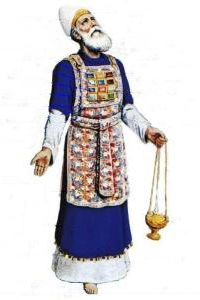
\includegraphics[width=50mm,scale=1.5]{Extras/Melchisedec.jpg}
\vspace{0.4in}  % Create a title for the document and write it in bold font
\LARGE{\textbf{\date}} % Again, do a line break
\linebreak 
% Create a subtitle \large{with Outlines, Statistics, Cross References, and Notes}
\vspace{0.5in}
\begin{flushleft}
\LARGE{Day \#47: Wednesday, 16 February 2022  \\}\vspace{0.25in}
\LARGE{Numbers 19-21 Psalm 47 Proverb 16}
\end{flushleft}
\vspace{0.6in}
\bigskip

\normalsize{Xenia, Oh.\\}
\normalsize{created: \today}
\vspace{1.3in}

\end{flushright}
\end{titlepage}

\newpage 
\tableofcontents\hypertarget{TOC}{}
\listoffigures
\listoftables

\hyphenation{A-bim-e-lech bre-thren E-phra-im  Gib-e-o-nites Jer-u-sa-lem through-out Phil-i-stines The-o-phil-us Am-a-le-kites ven-geance Mesh-el-e-mi-ah onan-ism Phar-a-oh thoughts grev-ous-ness Hach-a-liah adul-ter-er Shad-rach}

%%%%%%%%%%%%%%%%% EXTRA COLORS
%%%%%%%%%%%%%%%%% EXTRA COLORS
%%%%%%%%%%%%%%%%% EXTRA COLORS
\definecolor{champagne}{rgb}{0.97,0.91,0.81}
\definecolor{bone}{rgb}{0.89,0.85,0.79}

\definecolor{ForestGreen}{rgb}{0.00,0.29,0.098}
\definecolor{GIVING}{cmyk}{1,0.0,0.72,.1}

\definecolor{MLPE}{cmyk}{1,1,0,.45}
\definecolor{SOCCER}{cmyk}{.77, 0, .42, .49}
\definecolor{PAYBILL}{cmyk}{0,0.83,0.76,0.07}
\definecolor{SERMON}{cmyk}{.14,.9,0,.30} % aka seance \href{http://www.flatuicolorpicker.com/purple-cmyk-color-model/}{seance}
\definecolor{BIBLE}{cmyk}{0,.17,.74,.17}
\definecolor{WORKBLUE}{cmyk}{1, .5, 0, .6}
\definecolor{myOrange}{cmyk}{0, .4, .98, .03}
\definecolor{myTan}{cmyk}{0.0,.07,.17,.10}
\definecolor{myRed}{cmyk}{0,1,1,0}
\definecolor{myWhite}{cmyk}{0,0,0,0}
\definecolor{BLUESoD}{cmyk}{.97,.84,0,.04}
\definecolor{WHITE}{cmyk}{0,0,0,0}
\definecolor{OLDGOLD}{cmyk}{0.05,0.3,1.00,0}
\definecolor{CASTLETON}{cmyk}{1,0,0.31,0.66}
\definecolor{cadmiumgreen}{rgb}{0.0, 0.42, 0.24}
\definecolor{jungle}{rgb}{0.203,0.4882,0.1718}
\definecolor{MYGOLD}{rgb}{1,.84,0}

\definecolor{MYLIGHTGRAY}{rgb}{.85,.85,.85}

\definecolor{codegreen}{rgb}{0,0.6,0}
\definecolor{codegray}{rgb}{0.5,0.5,0.5}
\definecolor{codepurple}{rgb}{0.58,0,0.82}
\definecolor{backcolour}{rgb}{0.95,0.95,0.92}


\mdfdefinestyle{MyFrame}{%
    linecolor=blue,
    outerlinewidth=2pt,
    roundcorner=5pt,
    innertopmargin=\baselineskip,
    innerbottommargin=\baselineskip,
    innerrightmargin=10pt,
    innerleftmargin=10pt,
    backgroundcolor=gray!25!white}


\mdfdefinestyle{MyFrame2}{%
    linecolor=black,
    outerlinewidth=2pt,
    roundcorner=5pt,
    innertopmargin=\baselineskip,
    innerbottommargin=\baselineskip,
    innerrightmargin=10pt,
    innerleftmargin=10pt,
    backgroundcolor=yellow!25!white}


%%%%%
%% for PFTTIS list
%%%%%

%%% And Joseph said unto
\index[PFTTIS]{And Joseph said unto!Genesis!Gen 40:008}
\index[PFTTIS]{And Joseph said unto!Genesis!Gen 40:012}
\index[PFTTIS]{And Joseph said unto!Genesis!Gen 41:025}
\index[PFTTIS]{And Joseph said unto!Genesis!Gen 42:014}
\index[PFTTIS]{And Joseph said unto!Genesis!Gen 42:018}
\index[PFTTIS]{And Joseph said unto!Genesis!Gen 44:015}
\index[PFTTIS]{And Joseph said unto!Genesis!Gen 45:003}
\index[PFTTIS]{And Joseph said unto!Genesis!Gen 45:004}
\index[PFTTIS]{And Joseph said unto!Genesis!Gen 46:031}
\index[PFTTIS]{And Joseph said unto!Genesis!Gen 48:009}
\index[PFTTIS]{And Joseph said unto!Genesis!Gen 48:018}
\index[PFTTIS]{And Joseph said unto!Genesis!Gen 50:019}
\index[PFTTIS]{And Joseph said unto!Genesis!Gen 50:024}


%%% a shadow
\index[PFTTIS]{a shadow!1Chronicles!1Chr 029:15}
\index[PFTTIS]{a shadow!Job!Job 008:09}
\index[PFTTIS]{a shadow!Job!Job 014:02}
\index[PFTTIS]{a shadow!Job!Job 017:07}
\index[PFTTIS]{a shadow!Psalm!Psa 102:011}
\index[PFTTIS]{a shadow!Psalm!Psa 144:004}
\index[PFTTIS]{a shadow!Ecclesiastes!Eccl 006:012}
\index[PFTTIS]{a shadow!Ecclesiastes!Eccl 008:013}
\index[PFTTIS]{a shadow!Isaiah!Isa 04:006}
\index[PFTTIS]{a shadow!Isaiah!Isa 25:004}
\index[PFTTIS]{a shadow!Jonah!Jnh 04:06}
\index[PFTTIS]{a shadow!Colossians!Col 02:017}
\index[PFTTIS]{a shadow!Hebews!Heb 10:001}

%%% blessed is the man
\index[PFTTIS]{blessed is the man!Psalm!Psa 001:001}
\index[PFTTIS]{blessed is the man!Psalm!Psa 032:002}
\index[PFTTIS]{blessed is the man!Psalm!Psa 034:008}
\index[PFTTIS]{blessed is the man!Psalm!Psa 065:004}
\index[PFTTIS]{blessed is the man!Psalm!Psa 084:005}
\index[PFTTIS]{blessed is the man!Psalm!Psa 084:012}
\index[PFTTIS]{blessed is the man!Psalm!Psa 094:012}
\index[PFTTIS]{blessed is the man!Psalm!Psa 112:001}
\index[PFTTIS]{blessed is the man!Proverbs!Pro 008:034}
\index[PFTTIS]{blessed is the man!Isaiah!Isa 056:002}
\index[PFTTIS]{blessed is the man!Jeremiah!Jer 017:007}
\index[PFTTIS]{blessed is the man!Romans!Rom 004:008}
\index[PFTTIS]{blessed is the man!James!Jam 001:012}


%%% carry them
\index[PFTTIS]{carry them!Leviticus!Lev 14:045}
\index[PFTTIS]{carry them!Numbers!Num 11:012}
\index[PFTTIS]{carry them!Joshua!Jsh 04:003}
\index[PFTTIS]{carry them!1Samuel!1Sam 20:040}
\index[PFTTIS]{carry them!1Kings!1Kng 08:046}
\index[PFTTIS]{carry them!2Chronicles!2Chr 06:036}
\index[PFTTIS]{carry them!Ezra!Ezra 05:015}
\index[PFTTIS]{carry them!Isaiah!Isa 40:011}
\index[PFTTIS]{carry them!Isaiah!Isa 41:016}
\index[PFTTIS]{carry them!Isaiah!Isa 57:013}
\index[PFTTIS]{carry them!Jeremiah!Jer 20:004}
\index[PFTTIS]{carry them!Jeremiah!Jer 20:005}
\index[PFTTIS]{carry them!Jeremiah!Jer 43:012}


\index[PFTTIS]{good tidings!2Samuel!2Sam 18:027}
\index[PFTTIS]{good tidings!1Kings!1Ki 01:042}
\index[PFTTIS]{good tidings!2Kings!2Ki 07:009 (2x)}
\index[PFTTIS]{good tidings!Isaiah!Isa 40:009 (2x)}
\index[PFTTIS]{good tidings!Isaiah!Isa 41:007}
\index[PFTTIS]{good tidings!Isaiah!Isa 52:007}
\index[PFTTIS]{good tidings!Isaiah!Isa 61:001}
\index[PFTTIS]{good tidings!Nahum!Nah 01:005}
\index[PFTTIS]{good tidings!Luke!Lk 02:010}
\index[PFTTIS]{good tidings!1Thessalonians!1Thess 03:006}


%%% dead body
\index[PFTTIS]{dead body!Leviticus!Lev 21:011}
\index[PFTTIS]{dead body!Numbers!Num 06:006}
\index[PFTTIS]{dead body!Numbers!Num 09:006}
\index[PFTTIS]{dead body!Numbers!Num 09:007}
\index[PFTTIS]{dead body!Numbers!Num 09:010}
\index[PFTTIS]{dead body!Numbers!Num 09:011}
\index[PFTTIS]{dead body!Numbers!Num 09:013}
\index[PFTTIS]{dead body!Numbers!Num 09:016}
\index[PFTTIS]{dead body!2Kings!2Ki 08:005}
\index[PFTTIS]{dead body!Isaiah!Isa 26:019}
\index[PFTTIS]{dead body!Jeremiah!Jer 26:023}
\index[PFTTIS]{dead body!Jeremiah!Jer 36:030}
\index[PFTTIS]{dead body!Haggai!Hag 02:013}

%%% great sea
\index[PFTTIS]{great sea!Numbers!Num 34:006}
\index[PFTTIS]{great sea!Numbers!Num 34:007}
\index[PFTTIS]{great sea!Joshua!Jos 01:004}
\index[PFTTIS]{great sea!Joshua!Jos 09:001}
\index[PFTTIS]{great sea!Joshua!Jos 15:012}
\index[PFTTIS]{great sea!Joshua!Jos 15:047}
\index[PFTTIS]{great sea!Joshua!Jos 23:004}
\index[PFTTIS]{great sea!Ezekiel!Eze 47:010}
\index[PFTTIS]{great sea!Ezekiel!Eze 47:015}
\index[PFTTIS]{great sea!Ezekiel!Eze 47:019}
\index[PFTTIS]{great sea!Ezekiel!Eze 47:020}
\index[PFTTIS]{great sea!Ezekiel!Eze 48:028}
\index[PFTTIS]{great sea!Daniel!Dan 07:002}


%%% have forsaken me
\index[PFTTIS]{have forsaken me!Judges!Jdg 10:013}
\index[PFTTIS]{have forsaken me!1Samuel!1Sam 08:008}
\index[PFTTIS]{have forsaken me!1Kings!1Ki 11:033}
\index[PFTTIS]{have forsaken me!2Kings!2Ki 22:017}
\index[PFTTIS]{have forsaken me!2Chronicles!2Chr 12:005}
\index[PFTTIS]{have forsaken me!2Chronicles!2Chr 34:025}
\index[PFTTIS]{have forsaken me!Jeremiah!Jer 01:016}
\index[PFTTIS]{have forsaken me!Jeremiah!Jer 02:013}
\index[PFTTIS]{have forsaken me!Jeremiah!Jer 05:007}
\index[PFTTIS]{have forsaken me!Jeremiah!Jer 05:019}
\index[PFTTIS]{have forsaken me!Jeremiah!Jer 16:011 (2x)}
\index[PFTTIS]{have forsaken me!Jeremiah!Jer 19:004}

%%% no king
\index[PFTTIS]{no king!Judges!Jdg 17:06}
\index[PFTTIS]{no king!Judges!Jdg 18:01}
\index[PFTTIS]{no king!Judges!Jdg 19:01}
\index[PFTTIS]{no king!Judges!Jdg 21:25}
\index[PFTTIS]{no king!1Kings!1Ki 22:47}
\index[PFTTIS]{no king!2Kings!2Ki 23:25}
\index[PFTTIS]{no king!Nehemiah!Neh 13:26}
\index[PFTTIS]{no king!Psalms!Psa 033:016}
\index[PFTTIS]{no king!Proverbs!Pro 30:27}
\index[PFTTIS]{no king!Daniel!Dan 02:10}
\index[PFTTIS]{no king!Hosea!Hos 10:03}
\index[PFTTIS]{no king!Micah!Mic 04:09}
\index[PFTTIS]{no king!John!Jhn 19:15}


%%% rebellious house
\index[PFTTIS]{rebellious house!Exodus!Exo 02:005}
\index[PFTTIS]{rebellious house!Exodus!Exo 02:006}
\index[PFTTIS]{rebellious house!Exodus!Exo 02:008}
\index[PFTTIS]{rebellious house!Exodus!Exo 03:009}
\index[PFTTIS]{rebellious house!Exodus!Exo 03:026}
\index[PFTTIS]{rebellious house!Exodus!Exo 03:027}
\index[PFTTIS]{rebellious house!Exodus!Exo 12:002 (2x)}
\index[PFTTIS]{rebellious house!Exodus!Exo 12:003}
\index[PFTTIS]{rebellious house!Exodus!Exo 12:009}
\index[PFTTIS]{rebellious house!Exodus!Exo 12:025}
\index[PFTTIS]{rebellious house!Exodus!Exo 17:012}
\index[PFTTIS]{rebellious house!Exodus!Exo 24:003}

%%% seek him
\index[PFTTIS]{seek him!Deuteronomy!Deu 04:029}\index[PFTTIS]{seek him!1Samuel!1Sam 23:025}
\index[PFTTIS]{seek him!1Chronicles!1Chr 28:009}
\index[PFTTIS]{seek him!2Chronicles!1Chr 15:002}
\index[PFTTIS]{seek him!Ezra!Ezr 08:022}
\index[PFTTIS]{seek him!Psalms!Psa 022:026}
\index[PFTTIS]{seek him!Psalms!Psa 024:006}
\index[PFTTIS]{seek him!Psalms!Psa 119:002}
\index[PFTTIS]{seek him!SoS!SoS 03:002}
\index[PFTTIS]{seek him!SoS!SoS 06:001}
\index[PFTTIS]{seek him!Hosea!Hos 07:010}
\index[PFTTIS]{seek him!Amos!Amo 05:008}
\index[PFTTIS]{seek him!Hebrews!Heb 11:0063}


%%% seek ye
\index[PFTTIS]{seek ye!Isaiah!Isa 34:016}
\index[PFTTIS]{seek ye!Isaiah!Isa 45:019}
\index[PFTTIS]{seek ye!Isaiah!Isa 55:006}
\index[PFTTIS]{seek ye!Amos!Amos 5:004}
\index[PFTTIS]{seek ye!John!John 1:38}
\index[PFTTIS]{seek ye!John!John 18:4}
\index[PFTTIS]{seek ye!John!John 18:7}
\index[PFTTIS]{seek ye!Matthew!Matt 6:33}
\index[PFTTIS]{seek ye!Numbers!Num 16:10}
\index[PFTTIS]{seek ye!Luke!Luke 12:31}
\index[PFTTIS]{seek ye!Luke!Luke 24:5}
\index[PFTTIS]{seek ye!Psalm!Psa 27:8}
\index[PFTTIS]{seek ye!Zephaniah!Zeph 2:3}

%%% the uncircumcised
\index[PFTTIS]{the uncircumcised!Genesis!Gen 17:014}
\index[PFTTIS]{the uncircumcised!Judges!Jdg 14:003}
\index[PFTTIS]{the uncircumcised!Judges!Jdg 15:018}
\index[PFTTIS]{the uncircumcised!2Samuel!2Sam 01:020}
\index[PFTTIS]{the uncircumcised!Isaiah!Isa 02:001}
\index[PFTTIS]{the uncircumcised!Jeremiah!Jer 09:025}
\index[PFTTIS]{the uncircumcised!Ezekiel!Eze 28:010}
\index[PFTTIS]{the uncircumcised!Ezekiel!Eze 31:018}
\index[PFTTIS]{the uncircumcised!Ezekiel!Eze 32:019}
\index[PFTTIS]{the uncircumcised!Ezekiel!Eze 32:027}
\index[PFTTIS]{the uncircumcised!Ezekiel!Eze 32:028}
\index[PFTTIS]{the uncircumcised!Ezekiel!Eze 32:029}
\index[PFTTIS]{the uncircumcised!Ezekiel!Eze 32:032}

%%% worship him
\index[PFTTIS]{worship him!Psalms!Psa 97:007}
\index[PFTTIS]{worship him!Zephaniah!Zeph 02:011}
\index[PFTTIS]{worship him!Matthew!Matt 02:002}
\index[PFTTIS]{worship him!Matthew!Matt 02:008}
\index[PFTTIS]{worship him!John!John 04:023}
\index[PFTTIS]{worship him!John!John 04:024 (2x)} 
\index[PFTTIS]{worship him!Acts!Acts 17:023}
\index[PFTTIS]{worship him!Hebrews!Heb 01:006}
\index[PFTTIS]{worship him!Revelation!Rev 04:010}
\index[PFTTIS]{worship him!Revelation!Rev 13:008}
\index[PFTTIS]{worship him!Revelation!Rev 14:007}
\index[PFTTIS]{worship him!Revelation!Rev 19:010}


%%%%%
%% for PFTTIS list
%%%%%

%%% afflictions
\index[WFTTIS]{afflictions!Psalms!Psa 34:019}
\index[WFTTIS]{afflictions!Psalms!Psa 132:001}
\index[WFTTIS]{afflictions!Acts!Acts 07:010}
\index[WFTTIS]{afflictions!Acts!Acts 20:023}
\index[WFTTIS]{afflictions!2Corinthians!2Cor 06:004}
\index[WFTTIS]{afflictions!Colossians!Col 01:024}
\index[WFTTIS]{afflictions!1Thessalonians!1Thess 03:003}
\index[WFTTIS]{afflictions!2Timothy!2Tim 01:008}
\index[WFTTIS]{afflictions!2Timothy!2Tim 03:011}
\index[WFTTIS]{afflictions!2Timothy!2Tim 04:005}
\index[WFTTIS]{afflictions!Hebrews!Heb 10:032}
\index[WFTTIS]{afflictions!Hebrews!Heb 10:033}
\index[WFTTIS]{afflictions!1Peter!1Pet 05:009}

%%% acsend
\index[WFTTIS]{acsend!Joshua!Jos 06:05}
\index[WFTTIS]{acsend!Psalm!Psa 024:003}
\index[WFTTIS]{acsend!Psalm!Psa 135:007}
\index[WFTTIS]{acsend!Psalm!Psa 139:008}
\index[WFTTIS]{acsend!Isaiah!Isa 14:013}
\index[WFTTIS]{acsend!Isaiah!Isa 14:014}
\index[WFTTIS]{acsend!Jeremiah!Jer 10:013}
\index[WFTTIS]{acsend!Jeremiah!Jer 51:016}
\index[WFTTIS]{acsend!Ezekiel!Eze 38:009}
\index[WFTTIS]{acsend!John!John 06:062}
\index[WFTTIS]{acsend!John!John 20:017}
\index[WFTTIS]{acsend!Romans!Rom 10:006}
\index[WFTTIS]{acsend!Revelation!Rev 17:008}

%%% Assyrian
\index[WFTTIS]{Assyrian!Isaiah!Isa 10:005}
\index[WFTTIS]{Assyrian!Isaiah!Isa 10:024}
\index[WFTTIS]{Assyrian!Isaiah!Isa 14:025}
\index[WFTTIS]{Assyrian!Isaiah!Isa 19:023}
\index[WFTTIS]{Assyrian!Isaiah!Isa 23:013}
\index[WFTTIS]{Assyrian!Isaiah!Isa 30:031}
\index[WFTTIS]{Assyrian!Isaiah!Isa 31:008}
\index[WFTTIS]{Assyrian!Isaiah!Isa 52:004}
\index[WFTTIS]{Assyrian!Ezekiel!Eze 31:003}
\index[WFTTIS]{Assyrian!Hosea!Hos 05:013}
\index[WFTTIS]{Assyrian!Hosea!Hos 11:005}
\index[WFTTIS]{Assyrian!Micah!Hos 05:005}
\index[WFTTIS]{Assyrian!Micah!Hos 05:006}

%%% blot
\index[WFTTIS]{blot!Exodus!Exo 32:032}
\index[WFTTIS]{blot!Exodus!Exo 32:033}
\index[WFTTIS]{blot!Numbers!Num 05:026}
\index[WFTTIS]{blot!Deuteronomy!Deut 09:014}
\index[WFTTIS]{blot!Deuteronomy!Deut 25:019}
\index[WFTTIS]{blot!Deuteronomy!Deut 29:020}
\index[WFTTIS]{blot!2Kings!2Ki 14:027}
\index[WFTTIS]{blot!Job!Job 31:007}
\index[WFTTIS]{blot!Psalms!Psa 51:001}
\index[WFTTIS]{blot!Psalms!Psa 51:009}
\index[WFTTIS]{blot!Proverbs!Pro 09:007}
\index[WFTTIS]{blot!Jeremiah!Jer 18:023}
\index[WFTTIS]{blot!Revelation!Rev 03:005}


%%% chain
\index[WFTTIS]{chain!Genesis!Gen 41:042}
\index[WFTTIS]{chain!1Kings!1Ki 07:017}
\index[WFTTIS]{chain!Psalms!Psa 73:006}
\index[WFTTIS]{chain!SoS!Sos 04:009}
\index[WFTTIS]{chain!Lamentations!Lam 03:007}
\index[WFTTIS]{chain!Ezekiel!Eze 07:023}
\index[WFTTIS]{chain!Ezekiel!Eze 16:011}
\index[WFTTIS]{chain!Daniel!Dan 05:007}
\index[WFTTIS]{chain!Daniel!Dan 05:016}
\index[WFTTIS]{chain!Daniel!Dan 05:029}
\index[WFTTIS]{chain!Acts!Acts 28:020}
\index[WFTTIS]{chain!2Timothy!2Tim 01:016}
\index[WFTTIS]{chain!Revelation!Rev 20:001}


%%% controversy
\index[WFTTIS]{controversy!Deuteronomy!Deu 17:008}
\index[WFTTIS]{controversy!Deuteronomy!Deu 19:017}
\index[WFTTIS]{controversy!Deuteronomy!Deu 21:005}
\index[WFTTIS]{controversy!Deuteronomy!Deu 25:001}
\index[WFTTIS]{controversy!2Samuel!2Sam 15:002}
\index[WFTTIS]{controversy!Isaiah!Isa 34:008}
\index[WFTTIS]{controversy!Jeremiah!Jer 25:031}
\index[WFTTIS]{controversy!Ezekiel!Eze 44:024}
\index[WFTTIS]{controversy!Hosea!Hos 04:001}
\index[WFTTIS]{controversy!Hosea!Hos 12:002}
\index[WFTTIS]{controversy!Micah!Mic 06:002 (2x)}
\index[WFTTIS]{controversy!1Timothy!1Tim 03:016}


%%% Dagon/Dagon's
\index[WFTTIS]{Dagon!Judges!Jdg 16:023}
\index[WFTTIS]{Dagon!1Samuel!1Sam 05:002 (2x)}
\index[WFTTIS]{Dagon!1Samuel!1Sam 05:003 (2x)}
\index[WFTTIS]{Dagon!1Samuel!1Sam 05:004 (3x)}
\index[WFTTIS]{Dagon!1Samuel!1Sam 05:005 (3x)}
\index[WFTTIS]{Dagon!1Samuel!1Sam 05:007}
\index[WFTTIS]{Dagon!1Chronicles!1Chr 10:010}

%%% disobedient
\index[WFTTIS]{disobedient!1Kings!1Ki 13:026}
\index[WFTTIS]{disobedient!Nehemiah!Neh 09:026}
\index[WFTTIS]{disobedient!Luke!Luke 01:017}
\index[WFTTIS]{disobedient!Acts!Acts 26:019}
\index[WFTTIS]{disobedient!Romans!Rom 01:030}
\index[WFTTIS]{disobedient!Romans!Rom 10:021}
\index[WFTTIS]{disobedient!1Timothy!1Tim 01:009}
\index[WFTTIS]{disobedient!2Timothy!2Tim 03:002}
\index[WFTTIS]{disobedient!Titus!Titus 01:016}
\index[WFTTIS]{disobedient!Titus!Titus 03:003}
\index[WFTTIS]{disobedient!1Peter!1Pet 02:007}
\index[WFTTIS]{disobedient!1Peter!1Pet 02:008}
\index[WFTTIS]{disobedient!1Peter!1Pet 03:020}


%%% doubt
\index[WFTTIS]{doubt!Genesis!Gen 37:033}
\index[WFTTIS]{doubt!Deuteronomy!Deu 28:066}
\index[WFTTIS]{doubt!Job!Job 12:002}
\index[WFTTIS]{doubt!Matthew!Matt 14:031}
\index[WFTTIS]{doubt!Matthew!Matt 21:021}
\index[WFTTIS]{doubt!Mark!Mk 11:023}
\index[WFTTIS]{doubt!Luke!Lk 11:020}
\index[WFTTIS]{doubt!John!Jhn 10:024}
\index[WFTTIS]{doubt!Acts!Acts 02:012}
\index[WFTTIS]{doubt!Acts!Acts 28:004}
\index[WFTTIS]{doubt!1Corinthians!1Cor 09:010}
\index[WFTTIS]{doubt!Galatians!Gal 04:020}
\index[WFTTIS]{doubt!1John!1Jhn 02:019}


%%% dungeon
\index[WFTTIS]{dungeon!Genesis!Gen 40:015}
\index[WFTTIS]{dungeon!Genesis!Gen 41:014}
\index[WFTTIS]{dungeon!Exodus!Exo 12:029}
\index[WFTTIS]{dungeon!Jeremiah!Jer 37:016}
\index[WFTTIS]{dungeon!Jeremiah!Jer 38:006 (2x)}
\index[WFTTIS]{dungeon!Jeremiah!Jer 38:007}
\index[WFTTIS]{dungeon!Jeremiah!Jer 38:009}
\index[WFTTIS]{dungeon!Jeremiah!Jer 38:010}
\index[WFTTIS]{dungeon!Jeremiah!Jer 38:011}
\index[WFTTIS]{dungeon!Jeremiah!Jer 38:013}
\index[WFTTIS]{dungeon!Lamentations!Lam 03:053}
\index[WFTTIS]{dungeon!Lamentations!Lam 03:055}


%%% error
\index[WFTTIS]{error!2Samuel!2Sam 06:007}
\index[WFTTIS]{error!Job!Job 19:004}
\index[WFTTIS]{error!Ecclesiastes!Ecc 05:006}
\index[WFTTIS]{error!Ecclesiastes!Ecc 10:005}
\index[WFTTIS]{error!Isaiah!Isa 32:006}
\index[WFTTIS]{error!Daniel!Dan 06:004}
\index[WFTTIS]{error!Matthew!Matt 27:064}
\index[WFTTIS]{error!Romans!Rom 01:027}
\index[WFTTIS]{error!James!Jam 05:020}
\index[WFTTIS]{error!2Peter!2Pet 02:018}
\index[WFTTIS]{error!2Peter!2Pet 03:017}
\index[WFTTIS]{error!1John!1Jn 04:006}
\index[WFTTIS]{error!Jude!Jude 01:011}

%%% fourish
\index[WFTTIS]{fourish!Psalms!Psa 072:007}
\index[WFTTIS]{fourish!Psalms!Psa 072:016}
\index[WFTTIS]{fourish!Psalms!Psa 092:007}
\index[WFTTIS]{fourish!Psalms!Psa 092:012}
\index[WFTTIS]{fourish!Psalms!Psa 092:013}
\index[WFTTIS]{fourish!Psalms!Psa 132:018}
\index[WFTTIS]{fourish!Proverbs!Pro 11:28}
\index[WFTTIS]{fourish!Proverbs!Pro 14:11}
\index[WFTTIS]{fourish!Ecclesiastes!Ecc 12:05}
\index[WFTTIS]{fourish!SongOfSolomon!SOS 07:12}
\index[WFTTIS]{fourish!Isaiah!Isa 17:11}
\index[WFTTIS]{fourish!Isaiah!Isa 66:14}
\index[WFTTIS]{fourish!Ezekiel!Eze 17:24}




%%% giants
\index[WFTTIS]{giants!Genesis!Gen 06:004}
\index[WFTTIS]{giants!Numbers!Num 13:033}
\index[WFTTIS]{giants!Deuteronomy!Deut 02:011}
\index[WFTTIS]{giants!Deuteronomy!Deut 02:021}
\index[WFTTIS]{giants!Deuteronomy!Deut 03:011}
\index[WFTTIS]{giants!Deuteronomy!Deut 03:013}
\index[WFTTIS]{giants!Joshua!Josh 12:004}
\index[WFTTIS]{giants!Joshua!Josh 13:012}
\index[WFTTIS]{giants!Joshua!Josh 15:008}
\index[WFTTIS]{giants!Joshua!Josh 17:015}
\index[WFTTIS]{giants!Joshua!Josh 16:016}

%%% good man
\index[WFTTIS]{good man!2 Samuel!2Sa 18:27}
%(1) Psalms 37:23 [5]
%(1) Psalms 112:5 [2]
%(1) Proverbs 12:2 [2]
%(1) Proverbs 13:22 [2]
%(1) Proverbs 14:14 [14]
%(1) Micah 7:2 [2]
%(1) Matthew 12:35 [2]
%(1) Luke 6:45 [2]
%(1) Luke 23:50 [15]
%(1) John 7:12 [17]
%(1) Acts 11:24 [5]
%(1) Romans 5:7 [14]

%%% Hinnom
\index[WFTTIS]{Hinnom!Joshua!Jsh 15:008}
\index[WFTTIS]{Hinnom!Joshua!Jsh 18:016}
\index[WFTTIS]{Hinnom!2Kings!2Ki 23:010}
\index[WFTTIS]{Hinnom!2Chronicles!2Chr 28:003}
\index[WFTTIS]{Hinnom!2Chronicles!2Chr 33:006}
\index[WFTTIS]{Hinnom!Nehemiah!Neh 11:030}
\index[WFTTIS]{Hinnom!Jeremiah!Jer 07:031}
\index[WFTTIS]{Hinnom!Jeremiah!Jer 07:032}
\index[WFTTIS]{Hinnom!Jeremiah!Jer 19:002}
\index[WFTTIS]{Hinnom!Jeremiah!Jer 19:006}
\index[WFTTIS]{Hinnom!Jeremiah!Jer 32:035}

%%% inclined
\index[WFTTIS]{inclined!Judges!Jdg 09:003}
\index[WFTTIS]{inclined!Psalms!Psa 040:001}
\index[WFTTIS]{inclined!Psalms!Psa 116:002}
\index[WFTTIS]{inclined!Psalms!Psa 119:112}
\index[WFTTIS]{inclined!Proverbs!Pro 05:13}
\index[WFTTIS]{inclined!Jeremiah!Jer 07:24}
\index[WFTTIS]{inclined!Jeremiah!Jer 07:26}
\index[WFTTIS]{inclined!Jeremiah!Jer 11:08}
\index[WFTTIS]{inclined!Jeremiah!Jer 17:23}
\index[WFTTIS]{inclined!Jeremiah!Jer 25:04}
\index[WFTTIS]{inclined!Jeremiah!Jer 34:14}
\index[WFTTIS]{inclined!Jeremiah!Jer 35:15}
\index[WFTTIS]{inclined!Jeremiah!Jer 44:05}


%%% laughed
\index[WFTTIS]{laughed!Genesis!Gen 17:017}
\index[WFTTIS]{laughed!Genesis!Gen 18:012}
\index[WFTTIS]{laughed!Genesis!Gen 18:015}
\index[WFTTIS]{laughed!2Kings!2Ki 19:021}
\index[WFTTIS]{laughed!2Chronicles!2Chr 30:010}
\index[WFTTIS]{laughed!Nehemiah!Neh 02:019}
\index[WFTTIS]{laughed!Job!Job 12:004}
\index[WFTTIS]{laughed!Job!Job 29:024}
\index[WFTTIS]{laughed!Isaiah!Isa 37:022}
\index[WFTTIS]{laughed!Ezekiel!Ezek 23:032}
\index[WFTTIS]{laughed!Matthew!Matt 09:024}
\index[WFTTIS]{laughed!Mark!Mk 05:040}
\index[WFTTIS]{laughed!Luke!Lk 08:053}

%%% liar
\index[WFTTIS]{liar!Job!Job 24:025}
\index[WFTTIS]{liar!Proverbs!Pro 17:004}
\index[WFTTIS]{liar!Proverbs!Pro 19:022}
\index[WFTTIS]{liar!Proverbs!Pro 30:006}
\index[WFTTIS]{liar!Jeremiah!Jer 15:018}
\index[WFTTIS]{liar!John!Jhn 08:044}
\index[WFTTIS]{liar!John!Jhn 08:055}
\index[WFTTIS]{liar!Romans!Rom 03:004}
\index[WFTTIS]{liar!1John!1Jhn 01:010}
\index[WFTTIS]{liar!1John!1Jhn 02:004}
\index[WFTTIS]{liar!1John!1Jhn 02:022}
\index[WFTTIS]{liar!1John!1Jhn 04:020}
\index[WFTTIS]{liar!1John!1Jhn 05:010}

%%% palsy
\index[WFTTIS]{palsy!Matthew!Matt 04:024}
\index[WFTTIS]{palsy!Matthew!Matt 08:006}
\index[WFTTIS]{palsy!Matthew!Matt 09:002}
\index[WFTTIS]{palsy!Matthew!Matt 09:006}
\index[WFTTIS]{palsy!Mark!Mk 02:003}
\index[WFTTIS]{palsy!Mark!Mk 02:004}
\index[WFTTIS]{palsy!Mark!Mk 02:005}
\index[WFTTIS]{palsy!Mark!Mk 02:009}
\index[WFTTIS]{palsy!Mark!Mk 02:010}
\index[WFTTIS]{palsy!Luke!Lk 05:018}
\index[WFTTIS]{palsy!Luke!Lk 05:024}
\index[WFTTIS]{palsy!Acts!Acts 09:033}

%%% Profitable
\index[WFTTIS]{profitable!Job!Job 22:002 (2x)}
\index[WFTTIS]{profitable!Ecclesiastes!Ecc 10:010}
\index[WFTTIS]{profitable!Isaiah!Isa 44:010}
\index[WFTTIS]{profitable!Jeremiah!Jer 13:007}
\index[WFTTIS]{profitable!Matthew!Matt 05:029}
\index[WFTTIS]{profitable!Matthew!Matt 05:030}
\index[WFTTIS]{profitable!Acts!Acts 20:020}
\index[WFTTIS]{profitable!1Timothy!1Tim 04:008}
\index[WFTTIS]{profitable!2Timothy!2Tim 03:016}
\index[WFTTIS]{profitable!2Timothy!2Tim 04:011}
\index[WFTTIS]{profitable!Titus!Titus 03:008}
\index[WFTTIS]{profitable!Philemon!Phlm 01:011}

%%% Rechab
\index[WFTTIS]{Rechab!2Samuel!2Sam 04:002}
\index[WFTTIS]{Rechab!2Samuel!2Sam 04:005}
\index[WFTTIS]{Rechab!2Samuel!2Sam 04:006}
\index[WFTTIS]{Rechab!2Samuel!2Sam 04:009}
\index[WFTTIS]{Rechab!2KIngs!2Ki 10:015}
\index[WFTTIS]{Rechab!2KIngs!2Ki 10:023}
\index[WFTTIS]{Rechab!1Chronicles!1Chr 02:055}
\index[WFTTIS]{Rechab!Nehemiah!Neh 03:014}
\index[WFTTIS]{Rechab!Jeremiah!Jer 35:006}
\index[WFTTIS]{Rechab!Jeremiah!Jer 35:008}
\index[WFTTIS]{Rechab!Jeremiah!Jer 35:014}
\index[WFTTIS]{Rechab!Jeremiah!Jer 35:016}
\index[WFTTIS]{Rechab!Jeremiah!Jer 35:019}

%%% serpents
\index[WFTTIS]{serpents!Exodus!Exo 07:012}
\index[WFTTIS]{serpents!Numbers!Num 21:006}
\index[WFTTIS]{serpents!Numbers!Num 21:007}
\index[WFTTIS]{serpents!Deuteronomy!Deu 08:015}
\index[WFTTIS]{serpents!Deuteronomy!Deu 32:024}
\index[WFTTIS]{serpents!Jeremiah!Jer 08:017}
\index[WFTTIS]{serpents!Matthew!Matt 10:016}
\index[WFTTIS]{serpents!Matthew!Matt 23:033}
\index[WFTTIS]{serpents!Mark!Mk 16:018}
\index[WFTTIS]{serpents!Luke!Lk 10:019}
\index[WFTTIS]{serpents!1Corinthians!1Cor 10:009}
\index[WFTTIS]{serpents!James!Jas 03:007}
\index[WFTTIS]{serpents!Revelation!Rev 09:019}

%%% short
\index[WFTTIS]{short!Numbers!Num 11:023}
\index[WFTTIS]{short!2Kings!2Ki 10:032}
\index[WFTTIS]{short!Job!Job 17:012}
\index[WFTTIS]{short!Job!Job 20:005}
\index[WFTTIS]{short!Psalms!Psa 89:047}
\index[WFTTIS]{short!Romans!Rom 03:023}
\index[WFTTIS]{short!Romans!Rom 09:028  (2x)}
\index[WFTTIS]{short!1Corinthians!1Cor 07:029}
\index[WFTTIS]{short!1Thessalonians!1Thess 02:017}
\index[WFTTIS]{short!Hebrews!Heb 04:001}
\index[WFTTIS]{short!Revelation!Rev 12:012}
\index[WFTTIS]{short!Revelation!Rev 17:010}

%%% smiteth
\index[WFTTIS]{smiteth!Exodus!Exo 21:012}
\index[WFTTIS]{smiteth!Exodus!Exo 21:15}
\index[WFTTIS]{smiteth!Deuteronomy!Dt 25:11}
\index[WFTTIS]{smiteth!Deuteronomy!Dt 27:24}
\index[WFTTIS]{smiteth!Joshua!Jsh 15:16}
\index[WFTTIS]{smiteth!Judges!Jdg 15:16}
\index[WFTTIS]{smiteth!2 Samuel!2Sa 05:08}
\index[WFTTIS]{smiteth!1Chronicles!1Chr 11:06}
\index[WFTTIS]{smiteth!Job!1Chr 26:12}
\index[WFTTIS]{smiteth!Isaiah!Isa 09:13}
\index[WFTTIS]{smiteth!Lamentations!Lam 03:30}
\index[WFTTIS]{smiteth!Ezekiel!Eze 07:09}
\index[WFTTIS]{smiteth!Luke!Lk 06:29}



%%% vanities
\index[WFTTIS]{vanities!Deuteronomy!Deut 21:021}
\index[WFTTIS]{vanities!1Kings!1Ki 16:013}
\index[WFTTIS]{vanities!1Kings!1Ki 16:026}
\index[WFTTIS]{vanities!Psalms!Psa 031:006}
\index[WFTTIS]{vanities!Ecclesiastes!Ecc 01:002 (2x)}
\index[WFTTIS]{vanities!Ecclesiastes!Ecc 05:007}
\index[WFTTIS]{vanities!Ecclesiastes!Ecc 12:008}
\index[WFTTIS]{vanities!Jeremiah!Jer 08:019}
\index[WFTTIS]{vanities!Jeremiah!Jer 10:008}
\index[WFTTIS]{vanities!Jeremiah!Jer 14:022}
\index[WFTTIS]{vanities!Jonah!Jnh 02:008}
\index[WFTTIS]{vanities!Acts!Acts 14:015}



%%%%%
%% for PFTTIS list
%%%%%

%%% worm
\index[WFITV]{worm!Exodus!Exo 16:024}
\index[WFITV]{worm!Job!Job 17:014}
\index[WFITV]{worm!Job!Job 24:029}
\index[WFITV]{worm!Job!Job 25:005 (2x)}
\index[WFITV]{worm!Psalms!Psa 022:006}
\index[WFITV]{worm!Isaiah!Isa 14:011}
\index[WFITV]{worm!Isaiah!Isa 41:014}
\index[WFITV]{worm!Isaiah!Isa 51:008}
\index[WFITV]{worm!Isaiah!Isa 66:024}
\index[WFITV]{worm!Jonah!Jnh 04:007}
\index[WFITV]{worm!Mark!Mk 09:044}
\index[WFITV]{worm!Mark!Mk 09:046}
\index[WFITV]{worm!Mark!Mk 09:048}


%\subsubsection{Title}
%\textbf{Introduction:} Isaiah 46 
%\index[speaker]{Speaker!Isaiah 49 (Title}
%\index[series]{Book (Speaker)!IPassage (Title)}
%\index[date]{2017/07/09!Isaiah 49 (Title)}
%\begin{compactenum}[I.]
%    \item  \textbf{Point} \index[scripture]{Isaiah!IPassage} (IPassage)
%\end{compactenum}




  


%\input{02OT-Exodus/ExodusIntroduction}
\newpage
\begin{figure}
\begin{center}
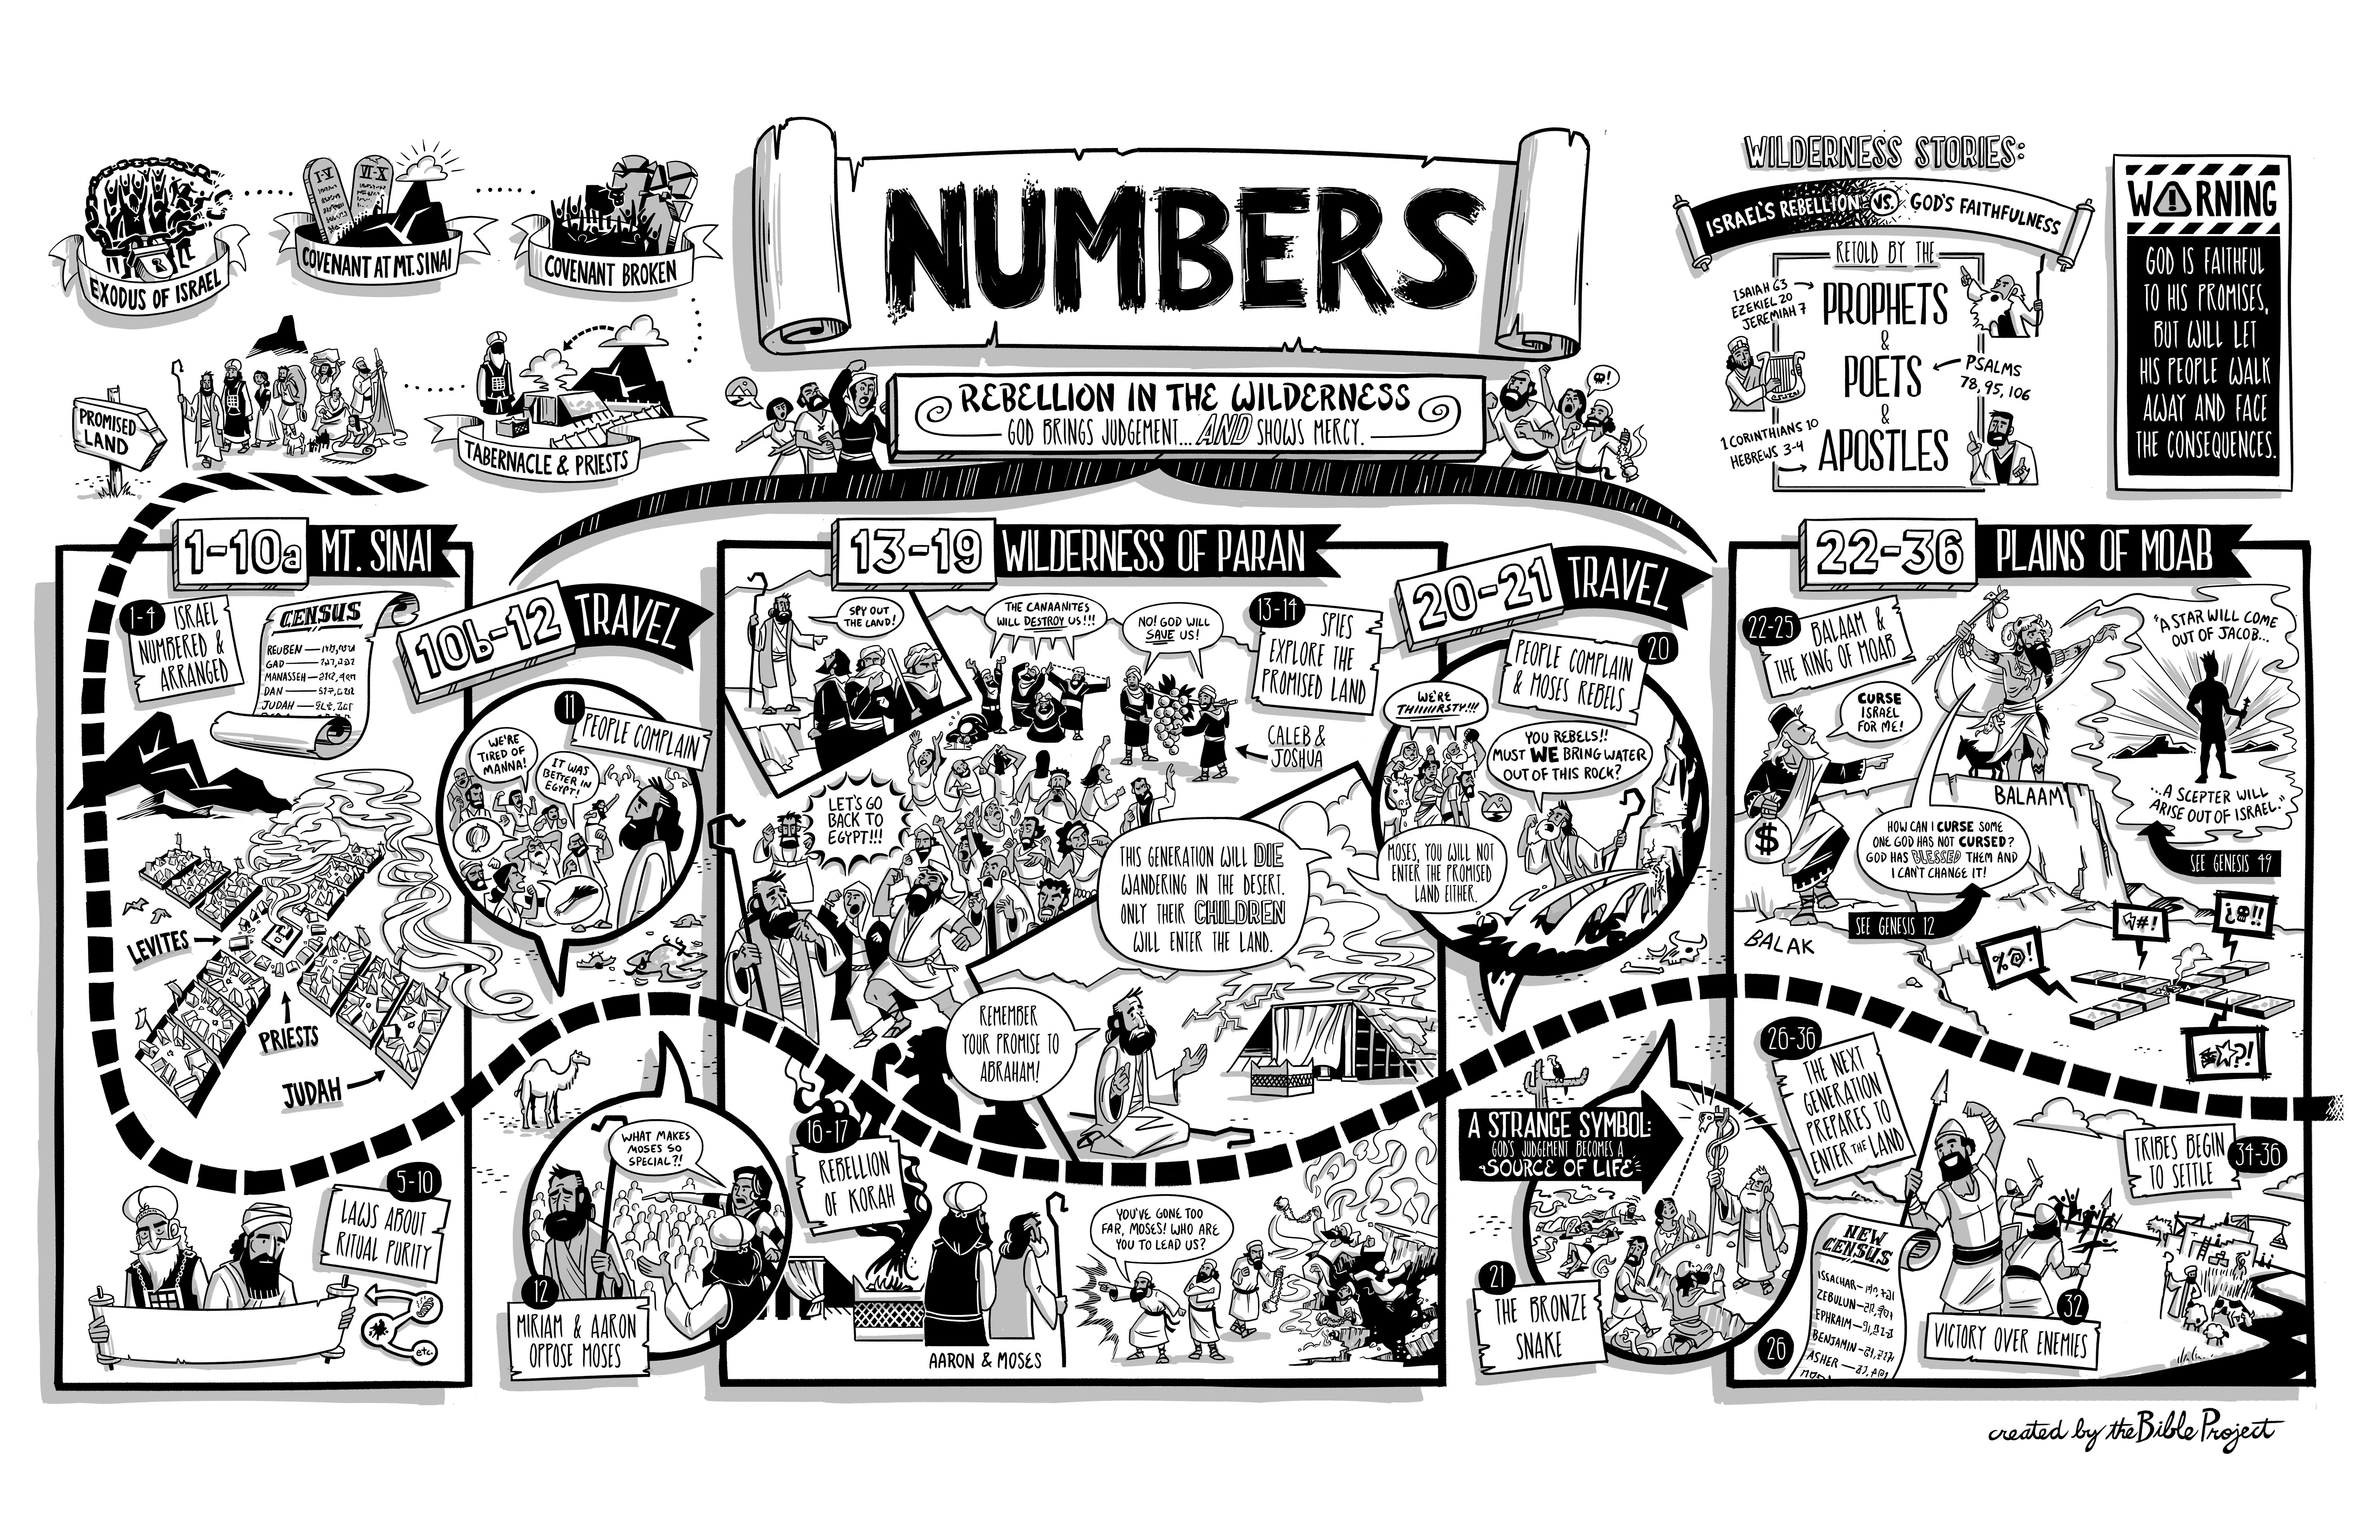
\includegraphics[scale=0.5, angle=90]{04OT-Numbers/References/BibleProject-Numbers.jpg}
\caption[Numbers from the Bible Project]{Numbers from the Bible Project}
\label{fig:Numbers from the Bible Project}
\end{center}
\end{figure}

\newpage
\begin{figure}
\begin{center}
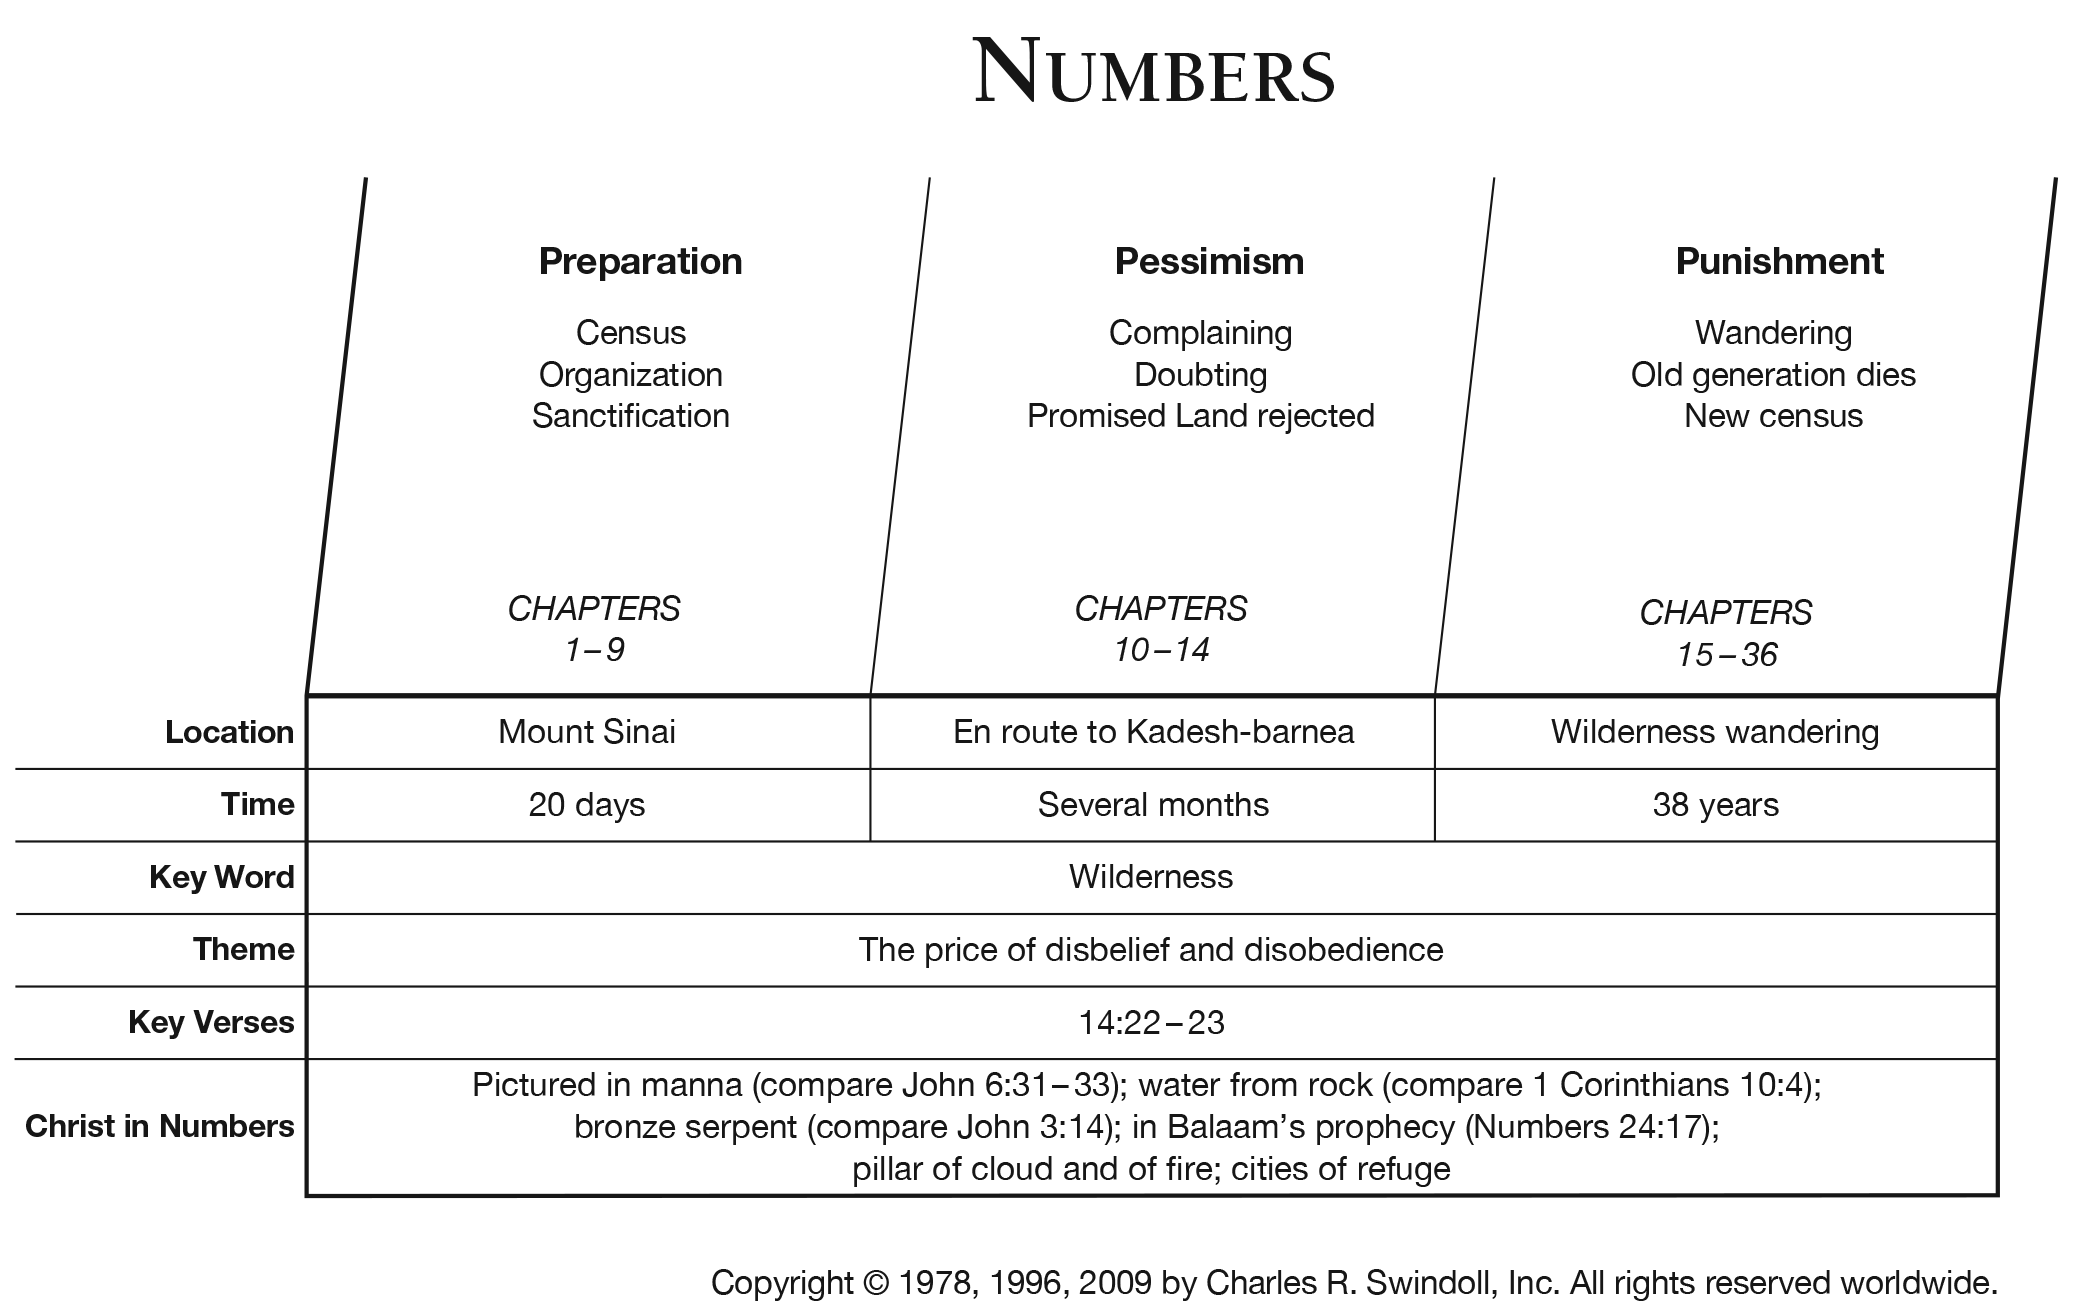
\includegraphics[scale=0.3, angle=90]{04OT-Numbers/References/Swindoll-Numbers.png}
\caption[Numbers by Swindoll]{Numbers by Swindoll}
\label{fig:Numbers by Swindoll}
\end{center}
\end{figure}

\newpage
\begin{figure}
\begin{center}
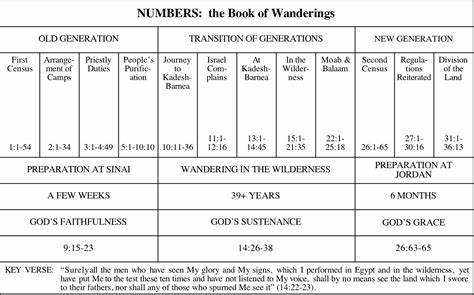
\includegraphics[scale=1.2, angle=90]{04OT-Numbers/References/Numbers.jpg}
\caption[Numbers by Unknown]{Numbers by Unknown}
\label{fig:Numbers by Unknown}
\end{center}
\end{figure}

\newpage
\begin{figure}
\begin{center}
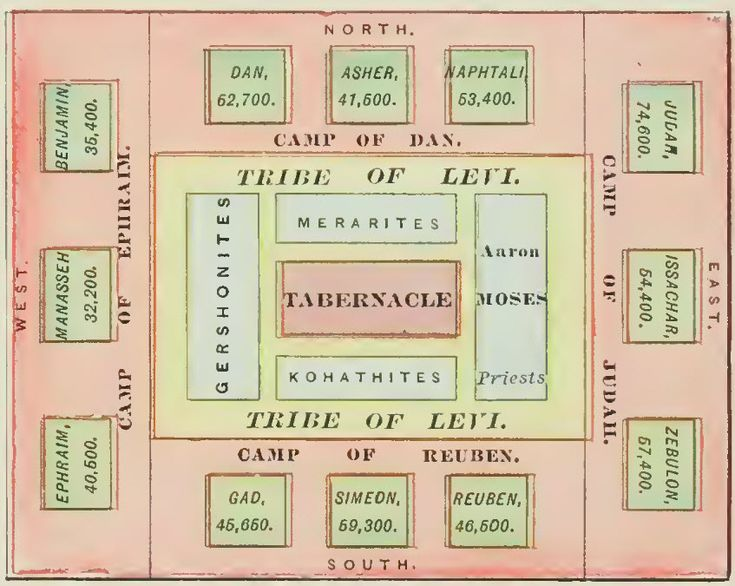
\includegraphics[scale=.8, angle=0]{04OT-Numbers/References/LayoutOfTribesAndTabernacle.jpg}
\caption[Layout of Tribes and Tabernacle]{Layout of Tribes and Tabernacle}
\label{fig:Layout of Tribes and Tabernacle}
\end{center}
\end{figure}


\chapter{Numbers 19}

\begin{figure}
  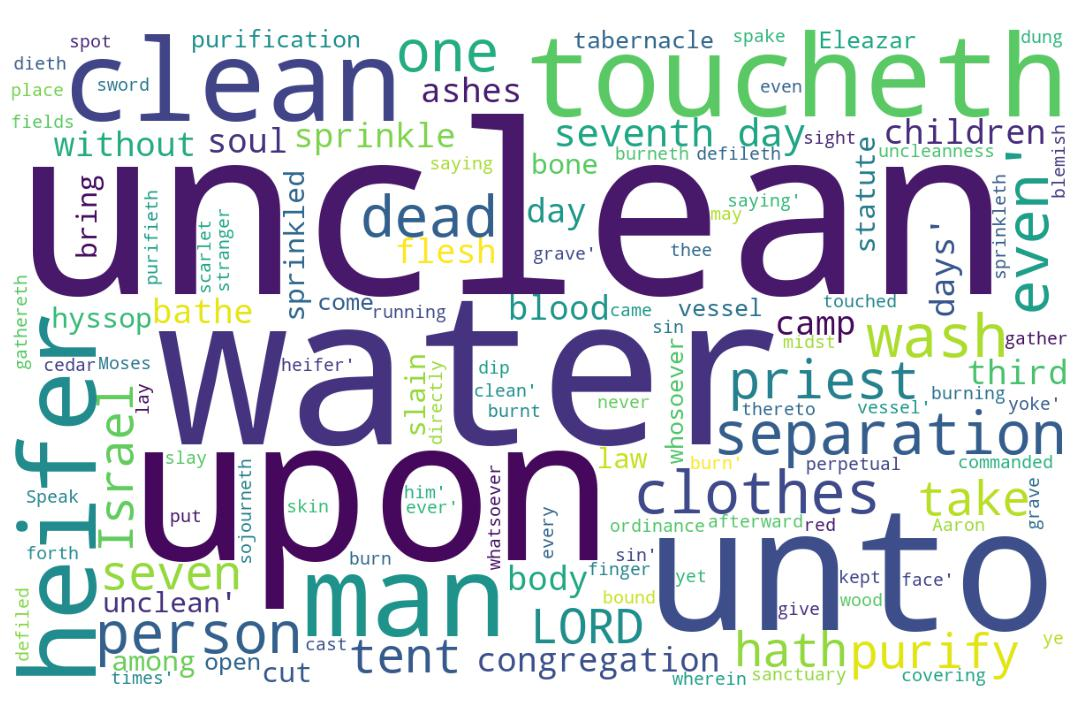
\includegraphics[width=\linewidth]{04OT-Numbers/Numbers19-WordCloud.jpg}
  \caption{Numbers 19 Word Cloud}
  \label{fig:Numbers 19 word Cloud}
\end{figure}



\marginpar{\scriptsize \centering \fcolorbox{bone}{lime}{\textbf{A RED HIEFER}}\\ (Numbers 19)
\begin{compactenum}[I.][8]
    \item  \textbf{Days} \index[scripture]{Numbers!Num 19:11} \index[scripture]{Numbers!Num 19:12} \index[scripture]{Numbers!Num 19:14}\index[scripture]{Numbers!Num 19:16}\index[scripture]{Numbers!Num 19:19} (Numbers 19:11, 12, 14, 16, 19) -- the typology of the third day and the seventh day
    \item  \textbf{Defilement} \index[scripture]{Numbers!Num 19:13} \index[scripture]{Numbers!Num 19:20} (Numbers 19:13, 20) 
    \item  \textbf{Destinations} \index[scripture]{Numbers!Num 19:03} \index[scripture]{Numbers!Num 19:07}\index[scripture]{Numbers!Num 19:09} (Numbers 19:3, 7, 9) -- inside the camp, outside the camp
    \item  \textbf{Designees}  -- the priest, the clean person, the unclean person, the dead body
    \item  \textbf{Ordinance}  \index[scripture]{Numbers!Num 19:02} (Numbers 19:2) 
    \item  \textbf{Defect} Free \index[scripture]{Numbers!Num 19:02} (Numbers 19:2) 
\end{compactenum}}

%[cmyk]{0.99998,1,0,0}{

\footnote{\textcolor[rgb]{0.00,0.25,0.00}{\hyperlink{NumbersTOC}{Return to end of Table of Contents.}}}\footnote{\href{https://audiobible.com/bible/numbers_19.html}{\textcolor[cmyk]{0.99998,1,0,0}{Numbers 19 Audio}}}\textcolor[cmyk]{0.99998,1,0,0}{And the LORD spake unto Moses and unto Aaron, saying,}
[2] \textcolor[cmyk]{0.99998,1,0,0}{This \emph{is} the ordinance of the law which the LORD hath commanded, saying, Speak unto the children of Israel, that they bring thee a red heifer without spot, wherein \emph{is} no blemish, \emph{and} upon which never came yoke:}
[3] \textcolor[cmyk]{0.99998,1,0,0}{And ye shall give her unto Eleazar the priest, that he may bring her forth without the camp, and \emph{one} shall slay her before his face:}
[4] \textcolor[cmyk]{0.99998,1,0,0}{And Eleazar the priest shall take of her blood with his finger, and sprinkle of her blood directly before the tabernacle of the congregation seven times:}
[5] \textcolor[cmyk]{0.99998,1,0,0}{And \emph{one} shall burn the heifer in his sight; her skin, and her flesh, and her blood, with her dung, shall he burn:}
[6] \textcolor[cmyk]{0.99998,1,0,0}{And the priest shall take cedar wood, and hyssop, and scarlet, and cast \emph{it} into the midst of the burning of the heifer.}
[7] \textcolor[cmyk]{0.99998,1,0,0}{Then the priest shall wash his clothes, and he shall bathe his flesh in water, and afterward he shall come into the camp, and the priest shall be unclean until the even.}
[8] \textcolor[cmyk]{0.99998,1,0,0}{And he that burneth her shall wash his clothes in water, and bathe his flesh in water, and shall be unclean until the even.}
[9] \textcolor[cmyk]{0.99998,1,0,0}{And a man \emph{that} \emph{is} clean shall gather up the ashes of the heifer, and lay \emph{them} up without the camp in a clean place, and it shall be kept for the congregation of the children of Israel for a water of separation: it \emph{is} a purification for sin.}
[10] \textcolor[cmyk]{0.99998,1,0,0}{And he that gathereth the ashes of the heifer shall wash his clothes, and be unclean until the even: and it shall be unto the children of Israel, and unto the stranger that sojourneth among them, for a statute for ever.}\\
\\
\P \textcolor[cmyk]{0.99998,1,0,0}{He that toucheth the dead body of any man shall be unclean seven days.}
[12] \textcolor[cmyk]{0.99998,1,0,0}{He shall purify himself with it on the third day, and on the seventh day he shall be clean: but if he purify not himself the third day, then the seventh day he shall not be clean.}
[13] \textcolor[cmyk]{0.99998,1,0,0}{Whosoever toucheth the dead body of any man that is dead, and purifieth not himself, defileth the tabernacle of the LORD; and that soul shall be cut off from Israel: because the water of separation was not sprinkled upon him, he shall be unclean; his uncleanness \emph{is} yet upon him.}
[14] \textcolor[cmyk]{0.99998,1,0,0}{This \emph{is} the law, when a man dieth in a tent: all that come into the tent, and all that \emph{is} in the tent, shall be unclean seven days.}
[15] \textcolor[cmyk]{0.99998,1,0,0}{And every open vessel, which hath no covering bound upon it, \emph{is} unclean.}
[16] \textcolor[cmyk]{0.99998,1,0,0}{And whosoever toucheth one that is slain with a sword in the open fields, or a dead body, or a bone of a man, or a grave, shall be unclean seven days.}
[17] \textcolor[cmyk]{0.99998,1,0,0}{And for an unclean \emph{person} they shall take of the ashes of the burnt heifer of purification for sin, and running water shall be put thereto in a vessel:}
[18] \textcolor[cmyk]{0.99998,1,0,0}{And a clean person shall take hyssop, and dip \emph{it} in the water, and sprinkle \emph{it} upon the tent, and upon all the vessels, and upon the persons that were there, and upon him that touched a bone, or one slain, or one dead, or a grave:}
[19] \textcolor[cmyk]{0.99998,1,0,0}{And the clean \emph{person} shall sprinkle upon the unclean on the third day, and on the seventh day: and on the seventh day he shall purify himself, and wash his clothes, and bathe himself in water, and shall be clean at even.}
[20] \textcolor[cmyk]{0.99998,1,0,0}{But the man that shall be unclean, and shall not purify himself, that soul shall be cut off from among the congregation, because he hath defiled the sanctuary of the LORD: the water of separation hath not been sprinkled upon him; he \emph{is} unclean.}
[21] \textcolor[cmyk]{0.99998,1,0,0}{And it shall be a perpetual statute unto them, that he that sprinkleth the water of separation shall wash his clothes; and he that toucheth the water of separation shall be unclean until even.}
[22] \textcolor[cmyk]{0.99998,1,0,0}{And whatsoever the unclean \emph{person} toucheth shall be unclean; and the soul that toucheth \emph{it} shall be unclean until even.}

\index[NWIV]{10!Numbers!Num 19:1}\index[AWIP]{And!Numbers!Num 19:1}\index[AWIP]{the!Numbers!Num 19:1}\index[AWIP]{LORD!Numbers!Num 19:1}\index[AWIP]{spake!Numbers!Num 19:1}\index[AWIP]{unto!Numbers!Num 19:1}\index[AWIP]{unto!Numbers!Num 19:1 (2)}\index[AWIP]{Moses!Numbers!Num 19:1}\index[AWIP]{and!Numbers!Num 19:1}\index[AWIP]{Aaron!Numbers!Num 19:1}\index[AWIP]{saying!Numbers!Num 19:1}

\index[NWIV]{38!Numbers!Num 19:2}\index[AWIP]{This!Numbers!Num 19:2}\index[AWIP]{\emph{is}!Numbers!Num 19:2}\index[AWIP]{\emph{is}!Numbers!Num 19:2 (2)}\index[AWIP]{the!Numbers!Num 19:2}\index[AWIP]{the!Numbers!Num 19:2 (2)}\index[AWIP]{the!Numbers!Num 19:2 (3)}\index[AWIP]{the!Numbers!Num 19:2 (4)}\index[AWIP]{ordinance!Numbers!Num 19:2}\index[AWIP]{of!Numbers!Num 19:2}\index[AWIP]{of!Numbers!Num 19:2 (2)}\index[AWIP]{law!Numbers!Num 19:2}\index[AWIP]{which!Numbers!Num 19:2}\index[AWIP]{which!Numbers!Num 19:2 (2)}\index[AWIP]{LORD!Numbers!Num 19:2}\index[AWIP]{hath!Numbers!Num 19:2}\index[AWIP]{commanded!Numbers!Num 19:2}\index[AWIP]{saying!Numbers!Num 19:2}\index[AWIP]{Speak!Numbers!Num 19:2}\index[AWIP]{unto!Numbers!Num 19:2}\index[AWIP]{children!Numbers!Num 19:2}\index[AWIP]{Israel!Numbers!Num 19:2}\index[AWIP]{that!Numbers!Num 19:2}\index[AWIP]{they!Numbers!Num 19:2}\index[AWIP]{bring!Numbers!Num 19:2}\index[AWIP]{thee!Numbers!Num 19:2}\index[AWIP]{a!Numbers!Num 19:2}\index[AWIP]{red!Numbers!Num 19:2}\index[AWIP]{heifer!Numbers!Num 19:2}\index[AWIP]{without!Numbers!Num 19:2}\index[AWIP]{spot!Numbers!Num 19:2}\index[AWIP]{wherein!Numbers!Num 19:2}\index[AWIP]{no!Numbers!Num 19:2}\index[AWIP]{blemish!Numbers!Num 19:2}\index[AWIP]{\emph{and}!Numbers!Num 19:2}\index[AWIP]{upon!Numbers!Num 19:2}\index[AWIP]{never!Numbers!Num 19:2}\index[AWIP]{came!Numbers!Num 19:2}\index[AWIP]{yoke!Numbers!Num 19:2}\index[AWIP]{\emph{is}!Numbers!Num 19:2}\index[AWIP]{\emph{is}!Numbers!Num 19:2 (2)}\index[AWIP]{\emph{and}!Numbers!Num 19:2}

\index[NWIV]{26!Numbers!Num 19:3}\index[AWIP]{And!Numbers!Num 19:3}\index[AWIP]{ye!Numbers!Num 19:3}\index[AWIP]{shall!Numbers!Num 19:3}\index[AWIP]{shall!Numbers!Num 19:3 (2)}\index[AWIP]{give!Numbers!Num 19:3}\index[AWIP]{her!Numbers!Num 19:3}\index[AWIP]{her!Numbers!Num 19:3 (2)}\index[AWIP]{her!Numbers!Num 19:3 (3)}\index[AWIP]{unto!Numbers!Num 19:3}\index[AWIP]{Eleazar!Numbers!Num 19:3}\index[AWIP]{the!Numbers!Num 19:3}\index[AWIP]{the!Numbers!Num 19:3 (2)}\index[AWIP]{priest!Numbers!Num 19:3}\index[AWIP]{that!Numbers!Num 19:3}\index[AWIP]{he!Numbers!Num 19:3}\index[AWIP]{may!Numbers!Num 19:3}\index[AWIP]{bring!Numbers!Num 19:3}\index[AWIP]{forth!Numbers!Num 19:3}\index[AWIP]{without!Numbers!Num 19:3}\index[AWIP]{camp!Numbers!Num 19:3}\index[AWIP]{and!Numbers!Num 19:3}\index[AWIP]{\emph{one}!Numbers!Num 19:3}\index[AWIP]{slay!Numbers!Num 19:3}\index[AWIP]{before!Numbers!Num 19:3}\index[AWIP]{his!Numbers!Num 19:3}\index[AWIP]{face!Numbers!Num 19:3}\index[AWIP]{\emph{one}!Numbers!Num 19:3}

\index[NWIV]{26!Numbers!Num 19:4}\index[AWIP]{And!Numbers!Num 19:4}\index[AWIP]{Eleazar!Numbers!Num 19:4}\index[AWIP]{the!Numbers!Num 19:4}\index[AWIP]{the!Numbers!Num 19:4 (2)}\index[AWIP]{the!Numbers!Num 19:4 (3)}\index[AWIP]{priest!Numbers!Num 19:4}\index[AWIP]{shall!Numbers!Num 19:4}\index[AWIP]{take!Numbers!Num 19:4}\index[AWIP]{of!Numbers!Num 19:4}\index[AWIP]{of!Numbers!Num 19:4 (2)}\index[AWIP]{of!Numbers!Num 19:4 (3)}\index[AWIP]{her!Numbers!Num 19:4}\index[AWIP]{her!Numbers!Num 19:4 (2)}\index[AWIP]{blood!Numbers!Num 19:4}\index[AWIP]{blood!Numbers!Num 19:4 (2)}\index[AWIP]{with!Numbers!Num 19:4}\index[AWIP]{his!Numbers!Num 19:4}\index[AWIP]{finger!Numbers!Num 19:4}\index[AWIP]{and!Numbers!Num 19:4}\index[AWIP]{sprinkle!Numbers!Num 19:4}\index[AWIP]{directly!Numbers!Num 19:4}\index[AWIP]{before!Numbers!Num 19:4}\index[AWIP]{tabernacle!Numbers!Num 19:4}\index[AWIP]{congregation!Numbers!Num 19:4}\index[AWIP]{seven!Numbers!Num 19:4}\index[AWIP]{times!Numbers!Num 19:4}

\index[NWIV]{23!Numbers!Num 19:5}\index[AWIP]{And!Numbers!Num 19:5}\index[AWIP]{\emph{one}!Numbers!Num 19:5}\index[AWIP]{shall!Numbers!Num 19:5}\index[AWIP]{shall!Numbers!Num 19:5 (2)}\index[AWIP]{burn!Numbers!Num 19:5}\index[AWIP]{burn!Numbers!Num 19:5 (2)}\index[AWIP]{the!Numbers!Num 19:5}\index[AWIP]{heifer!Numbers!Num 19:5}\index[AWIP]{in!Numbers!Num 19:5}\index[AWIP]{his!Numbers!Num 19:5}\index[AWIP]{sight!Numbers!Num 19:5}\index[AWIP]{her!Numbers!Num 19:5}\index[AWIP]{her!Numbers!Num 19:5 (2)}\index[AWIP]{her!Numbers!Num 19:5 (3)}\index[AWIP]{her!Numbers!Num 19:5 (4)}\index[AWIP]{skin!Numbers!Num 19:5}\index[AWIP]{and!Numbers!Num 19:5}\index[AWIP]{and!Numbers!Num 19:5 (2)}\index[AWIP]{flesh!Numbers!Num 19:5}\index[AWIP]{blood!Numbers!Num 19:5}\index[AWIP]{with!Numbers!Num 19:5}\index[AWIP]{dung!Numbers!Num 19:5}\index[AWIP]{he!Numbers!Num 19:5}\index[AWIP]{\emph{one}!Numbers!Num 19:5}

\index[NWIV]{23!Numbers!Num 19:6}\index[AWIP]{And!Numbers!Num 19:6}\index[AWIP]{the!Numbers!Num 19:6}\index[AWIP]{the!Numbers!Num 19:6 (2)}\index[AWIP]{the!Numbers!Num 19:6 (3)}\index[AWIP]{the!Numbers!Num 19:6 (4)}\index[AWIP]{priest!Numbers!Num 19:6}\index[AWIP]{shall!Numbers!Num 19:6}\index[AWIP]{take!Numbers!Num 19:6}\index[AWIP]{cedar!Numbers!Num 19:6}\index[AWIP]{wood!Numbers!Num 19:6}\index[AWIP]{and!Numbers!Num 19:6}\index[AWIP]{and!Numbers!Num 19:6 (2)}\index[AWIP]{and!Numbers!Num 19:6 (3)}\index[AWIP]{hyssop!Numbers!Num 19:6}\index[AWIP]{scarlet!Numbers!Num 19:6}\index[AWIP]{cast!Numbers!Num 19:6}\index[AWIP]{\emph{it}!Numbers!Num 19:6}\index[AWIP]{into!Numbers!Num 19:6}\index[AWIP]{midst!Numbers!Num 19:6}\index[AWIP]{of!Numbers!Num 19:6}\index[AWIP]{of!Numbers!Num 19:6 (2)}\index[AWIP]{burning!Numbers!Num 19:6}\index[AWIP]{heifer!Numbers!Num 19:6}\index[AWIP]{\emph{it}!Numbers!Num 19:6}

\index[NWIV]{32!Numbers!Num 19:7}\index[AWIP]{Then!Numbers!Num 19:7}\index[AWIP]{the!Numbers!Num 19:7}\index[AWIP]{the!Numbers!Num 19:7 (2)}\index[AWIP]{the!Numbers!Num 19:7 (3)}\index[AWIP]{the!Numbers!Num 19:7 (4)}\index[AWIP]{priest!Numbers!Num 19:7}\index[AWIP]{priest!Numbers!Num 19:7 (2)}\index[AWIP]{shall!Numbers!Num 19:7}\index[AWIP]{shall!Numbers!Num 19:7 (2)}\index[AWIP]{shall!Numbers!Num 19:7 (3)}\index[AWIP]{shall!Numbers!Num 19:7 (4)}\index[AWIP]{wash!Numbers!Num 19:7}\index[AWIP]{his!Numbers!Num 19:7}\index[AWIP]{his!Numbers!Num 19:7 (2)}\index[AWIP]{clothes!Numbers!Num 19:7}\index[AWIP]{and!Numbers!Num 19:7}\index[AWIP]{and!Numbers!Num 19:7 (2)}\index[AWIP]{and!Numbers!Num 19:7 (3)}\index[AWIP]{he!Numbers!Num 19:7}\index[AWIP]{he!Numbers!Num 19:7 (2)}\index[AWIP]{bathe!Numbers!Num 19:7}\index[AWIP]{flesh!Numbers!Num 19:7}\index[AWIP]{in!Numbers!Num 19:7}\index[AWIP]{water!Numbers!Num 19:7}\index[AWIP]{afterward!Numbers!Num 19:7}\index[AWIP]{come!Numbers!Num 19:7}\index[AWIP]{into!Numbers!Num 19:7}\index[AWIP]{camp!Numbers!Num 19:7}\index[AWIP]{be!Numbers!Num 19:7}\index[AWIP]{unclean!Numbers!Num 19:7}\index[AWIP]{until!Numbers!Num 19:7}\index[AWIP]{even!Numbers!Num 19:7}

\index[NWIV]{24!Numbers!Num 19:8}\index[AWIP]{And!Numbers!Num 19:8}\index[AWIP]{he!Numbers!Num 19:8}\index[AWIP]{that!Numbers!Num 19:8}\index[AWIP]{burneth!Numbers!Num 19:8}\index[AWIP]{her!Numbers!Num 19:8}\index[AWIP]{shall!Numbers!Num 19:8}\index[AWIP]{shall!Numbers!Num 19:8 (2)}\index[AWIP]{wash!Numbers!Num 19:8}\index[AWIP]{his!Numbers!Num 19:8}\index[AWIP]{his!Numbers!Num 19:8 (2)}\index[AWIP]{clothes!Numbers!Num 19:8}\index[AWIP]{in!Numbers!Num 19:8}\index[AWIP]{in!Numbers!Num 19:8 (2)}\index[AWIP]{water!Numbers!Num 19:8}\index[AWIP]{water!Numbers!Num 19:8 (2)}\index[AWIP]{and!Numbers!Num 19:8}\index[AWIP]{and!Numbers!Num 19:8 (2)}\index[AWIP]{bathe!Numbers!Num 19:8}\index[AWIP]{flesh!Numbers!Num 19:8}\index[AWIP]{be!Numbers!Num 19:8}\index[AWIP]{unclean!Numbers!Num 19:8}\index[AWIP]{until!Numbers!Num 19:8}\index[AWIP]{the!Numbers!Num 19:8}\index[AWIP]{even!Numbers!Num 19:8}

\index[NWIV]{49!Numbers!Num 19:9}\index[AWIP]{And!Numbers!Num 19:9}\index[AWIP]{a!Numbers!Num 19:9}\index[AWIP]{a!Numbers!Num 19:9 (2)}\index[AWIP]{a!Numbers!Num 19:9 (3)}\index[AWIP]{a!Numbers!Num 19:9 (4)}\index[AWIP]{man!Numbers!Num 19:9}\index[AWIP]{\emph{that}!Numbers!Num 19:9}\index[AWIP]{\emph{is}!Numbers!Num 19:9}\index[AWIP]{\emph{is}!Numbers!Num 19:9 (2)}\index[AWIP]{clean!Numbers!Num 19:9}\index[AWIP]{clean!Numbers!Num 19:9 (2)}\index[AWIP]{shall!Numbers!Num 19:9}\index[AWIP]{shall!Numbers!Num 19:9 (2)}\index[AWIP]{gather!Numbers!Num 19:9}\index[AWIP]{up!Numbers!Num 19:9}\index[AWIP]{up!Numbers!Num 19:9 (2)}\index[AWIP]{the!Numbers!Num 19:9}\index[AWIP]{the!Numbers!Num 19:9 (2)}\index[AWIP]{the!Numbers!Num 19:9 (3)}\index[AWIP]{the!Numbers!Num 19:9 (4)}\index[AWIP]{the!Numbers!Num 19:9 (5)}\index[AWIP]{ashes!Numbers!Num 19:9}\index[AWIP]{of!Numbers!Num 19:9}\index[AWIP]{of!Numbers!Num 19:9 (2)}\index[AWIP]{of!Numbers!Num 19:9 (3)}\index[AWIP]{of!Numbers!Num 19:9 (4)}\index[AWIP]{heifer!Numbers!Num 19:9}\index[AWIP]{and!Numbers!Num 19:9}\index[AWIP]{and!Numbers!Num 19:9 (2)}\index[AWIP]{lay!Numbers!Num 19:9}\index[AWIP]{\emph{them}!Numbers!Num 19:9}\index[AWIP]{without!Numbers!Num 19:9}\index[AWIP]{camp!Numbers!Num 19:9}\index[AWIP]{in!Numbers!Num 19:9}\index[AWIP]{place!Numbers!Num 19:9}\index[AWIP]{it!Numbers!Num 19:9}\index[AWIP]{it!Numbers!Num 19:9 (2)}\index[AWIP]{be!Numbers!Num 19:9}\index[AWIP]{kept!Numbers!Num 19:9}\index[AWIP]{for!Numbers!Num 19:9}\index[AWIP]{for!Numbers!Num 19:9 (2)}\index[AWIP]{for!Numbers!Num 19:9 (3)}\index[AWIP]{congregation!Numbers!Num 19:9}\index[AWIP]{children!Numbers!Num 19:9}\index[AWIP]{Israel!Numbers!Num 19:9}\index[AWIP]{water!Numbers!Num 19:9}\index[AWIP]{separation!Numbers!Num 19:9}\index[AWIP]{purification!Numbers!Num 19:9}\index[AWIP]{sin!Numbers!Num 19:9}\index[AWIP]{\emph{that}!Numbers!Num 19:9}\index[AWIP]{\emph{is}!Numbers!Num 19:9}\index[AWIP]{\emph{is}!Numbers!Num 19:9 (2)}\index[AWIP]{\emph{them}!Numbers!Num 19:9}

\index[NWIV]{41!Numbers!Num 19:10}\index[AWIP]{And!Numbers!Num 19:10}\index[AWIP]{he!Numbers!Num 19:10}\index[AWIP]{that!Numbers!Num 19:10}\index[AWIP]{that!Numbers!Num 19:10 (2)}\index[AWIP]{gathereth!Numbers!Num 19:10}\index[AWIP]{the!Numbers!Num 19:10}\index[AWIP]{the!Numbers!Num 19:10 (2)}\index[AWIP]{the!Numbers!Num 19:10 (3)}\index[AWIP]{the!Numbers!Num 19:10 (4)}\index[AWIP]{the!Numbers!Num 19:10 (5)}\index[AWIP]{ashes!Numbers!Num 19:10}\index[AWIP]{of!Numbers!Num 19:10}\index[AWIP]{of!Numbers!Num 19:10 (2)}\index[AWIP]{heifer!Numbers!Num 19:10}\index[AWIP]{shall!Numbers!Num 19:10}\index[AWIP]{shall!Numbers!Num 19:10 (2)}\index[AWIP]{wash!Numbers!Num 19:10}\index[AWIP]{his!Numbers!Num 19:10}\index[AWIP]{clothes!Numbers!Num 19:10}\index[AWIP]{and!Numbers!Num 19:10}\index[AWIP]{and!Numbers!Num 19:10 (2)}\index[AWIP]{and!Numbers!Num 19:10 (3)}\index[AWIP]{be!Numbers!Num 19:10}\index[AWIP]{be!Numbers!Num 19:10 (2)}\index[AWIP]{unclean!Numbers!Num 19:10}\index[AWIP]{until!Numbers!Num 19:10}\index[AWIP]{even!Numbers!Num 19:10}\index[AWIP]{it!Numbers!Num 19:10}\index[AWIP]{unto!Numbers!Num 19:10}\index[AWIP]{unto!Numbers!Num 19:10 (2)}\index[AWIP]{children!Numbers!Num 19:10}\index[AWIP]{Israel!Numbers!Num 19:10}\index[AWIP]{stranger!Numbers!Num 19:10}\index[AWIP]{sojourneth!Numbers!Num 19:10}\index[AWIP]{among!Numbers!Num 19:10}\index[AWIP]{them!Numbers!Num 19:10}\index[AWIP]{for!Numbers!Num 19:10}\index[AWIP]{for!Numbers!Num 19:10 (2)}\index[AWIP]{a!Numbers!Num 19:10}\index[AWIP]{statute!Numbers!Num 19:10}\index[AWIP]{ever!Numbers!Num 19:10}

\index[NWIV]{14!Numbers!Num 19:11}\index[AWIP]{He!Numbers!Num 19:11}\index[AWIP]{that!Numbers!Num 19:11}\index[AWIP]{toucheth!Numbers!Num 19:11}\index[AWIP]{the!Numbers!Num 19:11}\index[AWIP]{dead!Numbers!Num 19:11}\index[AWIP]{body!Numbers!Num 19:11}\index[AWIP]{of!Numbers!Num 19:11}\index[AWIP]{any!Numbers!Num 19:11}\index[AWIP]{man!Numbers!Num 19:11}\index[AWIP]{shall!Numbers!Num 19:11}\index[AWIP]{be!Numbers!Num 19:11}\index[AWIP]{unclean!Numbers!Num 19:11}\index[AWIP]{seven!Numbers!Num 19:11}\index[AWIP]{days!Numbers!Num 19:11}

\index[NWIV]{37!Numbers!Num 19:12}\index[AWIP]{He!Numbers!Num 19:12}\index[AWIP]{shall!Numbers!Num 19:12}\index[AWIP]{shall!Numbers!Num 19:12 (2)}\index[AWIP]{shall!Numbers!Num 19:12 (3)}\index[AWIP]{purify!Numbers!Num 19:12}\index[AWIP]{purify!Numbers!Num 19:12 (2)}\index[AWIP]{himself!Numbers!Num 19:12}\index[AWIP]{himself!Numbers!Num 19:12 (2)}\index[AWIP]{with!Numbers!Num 19:12}\index[AWIP]{it!Numbers!Num 19:12}\index[AWIP]{on!Numbers!Num 19:12}\index[AWIP]{on!Numbers!Num 19:12 (2)}\index[AWIP]{the!Numbers!Num 19:12}\index[AWIP]{the!Numbers!Num 19:12 (2)}\index[AWIP]{the!Numbers!Num 19:12 (3)}\index[AWIP]{the!Numbers!Num 19:12 (4)}\index[AWIP]{third!Numbers!Num 19:12}\index[AWIP]{third!Numbers!Num 19:12 (2)}\index[AWIP]{day!Numbers!Num 19:12}\index[AWIP]{day!Numbers!Num 19:12 (2)}\index[AWIP]{day!Numbers!Num 19:12 (3)}\index[AWIP]{day!Numbers!Num 19:12 (4)}\index[AWIP]{and!Numbers!Num 19:12}\index[AWIP]{seventh!Numbers!Num 19:12}\index[AWIP]{seventh!Numbers!Num 19:12 (2)}\index[AWIP]{he!Numbers!Num 19:12}\index[AWIP]{he!Numbers!Num 19:12 (2)}\index[AWIP]{he!Numbers!Num 19:12 (3)}\index[AWIP]{be!Numbers!Num 19:12}\index[AWIP]{be!Numbers!Num 19:12 (2)}\index[AWIP]{clean!Numbers!Num 19:12}\index[AWIP]{clean!Numbers!Num 19:12 (2)}\index[AWIP]{but!Numbers!Num 19:12}\index[AWIP]{if!Numbers!Num 19:12}\index[AWIP]{not!Numbers!Num 19:12}\index[AWIP]{not!Numbers!Num 19:12 (2)}\index[AWIP]{then!Numbers!Num 19:12}

\index[NWIV]{50!Numbers!Num 19:13}\index[AWIP]{Whosoever!Numbers!Num 19:13}\index[AWIP]{toucheth!Numbers!Num 19:13}\index[AWIP]{the!Numbers!Num 19:13}\index[AWIP]{the!Numbers!Num 19:13 (2)}\index[AWIP]{the!Numbers!Num 19:13 (3)}\index[AWIP]{the!Numbers!Num 19:13 (4)}\index[AWIP]{dead!Numbers!Num 19:13}\index[AWIP]{dead!Numbers!Num 19:13 (2)}\index[AWIP]{body!Numbers!Num 19:13}\index[AWIP]{of!Numbers!Num 19:13}\index[AWIP]{of!Numbers!Num 19:13 (2)}\index[AWIP]{of!Numbers!Num 19:13 (3)}\index[AWIP]{any!Numbers!Num 19:13}\index[AWIP]{man!Numbers!Num 19:13}\index[AWIP]{that!Numbers!Num 19:13}\index[AWIP]{that!Numbers!Num 19:13 (2)}\index[AWIP]{is!Numbers!Num 19:13}\index[AWIP]{and!Numbers!Num 19:13}\index[AWIP]{and!Numbers!Num 19:13 (2)}\index[AWIP]{purifieth!Numbers!Num 19:13}\index[AWIP]{not!Numbers!Num 19:13}\index[AWIP]{not!Numbers!Num 19:13 (2)}\index[AWIP]{himself!Numbers!Num 19:13}\index[AWIP]{defileth!Numbers!Num 19:13}\index[AWIP]{tabernacle!Numbers!Num 19:13}\index[AWIP]{LORD!Numbers!Num 19:13}\index[AWIP]{soul!Numbers!Num 19:13}\index[AWIP]{shall!Numbers!Num 19:13}\index[AWIP]{shall!Numbers!Num 19:13 (2)}\index[AWIP]{be!Numbers!Num 19:13}\index[AWIP]{be!Numbers!Num 19:13 (2)}\index[AWIP]{cut!Numbers!Num 19:13}\index[AWIP]{off!Numbers!Num 19:13}\index[AWIP]{from!Numbers!Num 19:13}\index[AWIP]{Israel!Numbers!Num 19:13}\index[AWIP]{because!Numbers!Num 19:13}\index[AWIP]{water!Numbers!Num 19:13}\index[AWIP]{separation!Numbers!Num 19:13}\index[AWIP]{was!Numbers!Num 19:13}\index[AWIP]{sprinkled!Numbers!Num 19:13}\index[AWIP]{upon!Numbers!Num 19:13}\index[AWIP]{upon!Numbers!Num 19:13 (2)}\index[AWIP]{him!Numbers!Num 19:13}\index[AWIP]{him!Numbers!Num 19:13 (2)}\index[AWIP]{he!Numbers!Num 19:13}\index[AWIP]{unclean!Numbers!Num 19:13}\index[AWIP]{his!Numbers!Num 19:13}\index[AWIP]{uncleanness!Numbers!Num 19:13}\index[AWIP]{\emph{is}!Numbers!Num 19:13}\index[AWIP]{yet!Numbers!Num 19:13}\index[AWIP]{\emph{is}!Numbers!Num 19:13}

\index[NWIV]{29!Numbers!Num 19:14}\index[AWIP]{This!Numbers!Num 19:14}\index[AWIP]{\emph{is}!Numbers!Num 19:14}\index[AWIP]{\emph{is}!Numbers!Num 19:14 (2)}\index[AWIP]{the!Numbers!Num 19:14}\index[AWIP]{the!Numbers!Num 19:14 (2)}\index[AWIP]{the!Numbers!Num 19:14 (3)}\index[AWIP]{law!Numbers!Num 19:14}\index[AWIP]{when!Numbers!Num 19:14}\index[AWIP]{a!Numbers!Num 19:14}\index[AWIP]{a!Numbers!Num 19:14 (2)}\index[AWIP]{man!Numbers!Num 19:14}\index[AWIP]{dieth!Numbers!Num 19:14}\index[AWIP]{in!Numbers!Num 19:14}\index[AWIP]{in!Numbers!Num 19:14 (2)}\index[AWIP]{tent!Numbers!Num 19:14}\index[AWIP]{tent!Numbers!Num 19:14 (2)}\index[AWIP]{tent!Numbers!Num 19:14 (3)}\index[AWIP]{all!Numbers!Num 19:14}\index[AWIP]{all!Numbers!Num 19:14 (2)}\index[AWIP]{that!Numbers!Num 19:14}\index[AWIP]{that!Numbers!Num 19:14 (2)}\index[AWIP]{come!Numbers!Num 19:14}\index[AWIP]{into!Numbers!Num 19:14}\index[AWIP]{and!Numbers!Num 19:14}\index[AWIP]{shall!Numbers!Num 19:14}\index[AWIP]{be!Numbers!Num 19:14}\index[AWIP]{unclean!Numbers!Num 19:14}\index[AWIP]{seven!Numbers!Num 19:14}\index[AWIP]{days!Numbers!Num 19:14}\index[AWIP]{\emph{is}!Numbers!Num 19:14}\index[AWIP]{\emph{is}!Numbers!Num 19:14 (2)}

\index[NWIV]{13!Numbers!Num 19:15}\index[AWIP]{And!Numbers!Num 19:15}\index[AWIP]{every!Numbers!Num 19:15}\index[AWIP]{open!Numbers!Num 19:15}\index[AWIP]{vessel!Numbers!Num 19:15}\index[AWIP]{which!Numbers!Num 19:15}\index[AWIP]{hath!Numbers!Num 19:15}\index[AWIP]{no!Numbers!Num 19:15}\index[AWIP]{covering!Numbers!Num 19:15}\index[AWIP]{bound!Numbers!Num 19:15}\index[AWIP]{upon!Numbers!Num 19:15}\index[AWIP]{it!Numbers!Num 19:15}\index[AWIP]{\emph{is}!Numbers!Num 19:15}\index[AWIP]{unclean!Numbers!Num 19:15}\index[AWIP]{\emph{is}!Numbers!Num 19:15}

\index[NWIV]{32!Numbers!Num 19:16}\index[AWIP]{And!Numbers!Num 19:16}\index[AWIP]{whosoever!Numbers!Num 19:16}\index[AWIP]{toucheth!Numbers!Num 19:16}\index[AWIP]{one!Numbers!Num 19:16}\index[AWIP]{that!Numbers!Num 19:16}\index[AWIP]{is!Numbers!Num 19:16}\index[AWIP]{slain!Numbers!Num 19:16}\index[AWIP]{with!Numbers!Num 19:16}\index[AWIP]{a!Numbers!Num 19:16}\index[AWIP]{a!Numbers!Num 19:16 (2)}\index[AWIP]{a!Numbers!Num 19:16 (3)}\index[AWIP]{a!Numbers!Num 19:16 (4)}\index[AWIP]{a!Numbers!Num 19:16 (5)}\index[AWIP]{sword!Numbers!Num 19:16}\index[AWIP]{in!Numbers!Num 19:16}\index[AWIP]{the!Numbers!Num 19:16}\index[AWIP]{open!Numbers!Num 19:16}\index[AWIP]{fields!Numbers!Num 19:16}\index[AWIP]{or!Numbers!Num 19:16}\index[AWIP]{or!Numbers!Num 19:16 (2)}\index[AWIP]{or!Numbers!Num 19:16 (3)}\index[AWIP]{dead!Numbers!Num 19:16}\index[AWIP]{body!Numbers!Num 19:16}\index[AWIP]{bone!Numbers!Num 19:16}\index[AWIP]{of!Numbers!Num 19:16}\index[AWIP]{man!Numbers!Num 19:16}\index[AWIP]{grave!Numbers!Num 19:16}\index[AWIP]{shall!Numbers!Num 19:16}\index[AWIP]{be!Numbers!Num 19:16}\index[AWIP]{unclean!Numbers!Num 19:16}\index[AWIP]{seven!Numbers!Num 19:16}\index[AWIP]{days!Numbers!Num 19:16}

\index[NWIV]{29!Numbers!Num 19:17}\index[AWIP]{And!Numbers!Num 19:17}\index[AWIP]{for!Numbers!Num 19:17}\index[AWIP]{for!Numbers!Num 19:17 (2)}\index[AWIP]{an!Numbers!Num 19:17}\index[AWIP]{unclean!Numbers!Num 19:17}\index[AWIP]{\emph{person}!Numbers!Num 19:17}\index[AWIP]{they!Numbers!Num 19:17}\index[AWIP]{shall!Numbers!Num 19:17}\index[AWIP]{shall!Numbers!Num 19:17 (2)}\index[AWIP]{take!Numbers!Num 19:17}\index[AWIP]{of!Numbers!Num 19:17}\index[AWIP]{of!Numbers!Num 19:17 (2)}\index[AWIP]{of!Numbers!Num 19:17 (3)}\index[AWIP]{the!Numbers!Num 19:17}\index[AWIP]{the!Numbers!Num 19:17 (2)}\index[AWIP]{ashes!Numbers!Num 19:17}\index[AWIP]{burnt!Numbers!Num 19:17}\index[AWIP]{heifer!Numbers!Num 19:17}\index[AWIP]{purification!Numbers!Num 19:17}\index[AWIP]{sin!Numbers!Num 19:17}\index[AWIP]{and!Numbers!Num 19:17}\index[AWIP]{running!Numbers!Num 19:17}\index[AWIP]{water!Numbers!Num 19:17}\index[AWIP]{be!Numbers!Num 19:17}\index[AWIP]{put!Numbers!Num 19:17}\index[AWIP]{thereto!Numbers!Num 19:17}\index[AWIP]{in!Numbers!Num 19:17}\index[AWIP]{a!Numbers!Num 19:17}\index[AWIP]{vessel!Numbers!Num 19:17}\index[AWIP]{\emph{person}!Numbers!Num 19:17}

\index[NWIV]{47!Numbers!Num 19:18}\index[AWIP]{And!Numbers!Num 19:18}\index[AWIP]{a!Numbers!Num 19:18}\index[AWIP]{a!Numbers!Num 19:18 (2)}\index[AWIP]{a!Numbers!Num 19:18 (3)}\index[AWIP]{clean!Numbers!Num 19:18}\index[AWIP]{person!Numbers!Num 19:18}\index[AWIP]{shall!Numbers!Num 19:18}\index[AWIP]{take!Numbers!Num 19:18}\index[AWIP]{hyssop!Numbers!Num 19:18}\index[AWIP]{and!Numbers!Num 19:18}\index[AWIP]{and!Numbers!Num 19:18 (2)}\index[AWIP]{and!Numbers!Num 19:18 (3)}\index[AWIP]{and!Numbers!Num 19:18 (4)}\index[AWIP]{and!Numbers!Num 19:18 (5)}\index[AWIP]{dip!Numbers!Num 19:18}\index[AWIP]{\emph{it}!Numbers!Num 19:18}\index[AWIP]{\emph{it}!Numbers!Num 19:18 (2)}\index[AWIP]{in!Numbers!Num 19:18}\index[AWIP]{the!Numbers!Num 19:18}\index[AWIP]{the!Numbers!Num 19:18 (2)}\index[AWIP]{the!Numbers!Num 19:18 (3)}\index[AWIP]{the!Numbers!Num 19:18 (4)}\index[AWIP]{water!Numbers!Num 19:18}\index[AWIP]{sprinkle!Numbers!Num 19:18}\index[AWIP]{upon!Numbers!Num 19:18}\index[AWIP]{upon!Numbers!Num 19:18 (2)}\index[AWIP]{upon!Numbers!Num 19:18 (3)}\index[AWIP]{upon!Numbers!Num 19:18 (4)}\index[AWIP]{tent!Numbers!Num 19:18}\index[AWIP]{all!Numbers!Num 19:18}\index[AWIP]{vessels!Numbers!Num 19:18}\index[AWIP]{persons!Numbers!Num 19:18}\index[AWIP]{that!Numbers!Num 19:18}\index[AWIP]{that!Numbers!Num 19:18 (2)}\index[AWIP]{were!Numbers!Num 19:18}\index[AWIP]{there!Numbers!Num 19:18}\index[AWIP]{him!Numbers!Num 19:18}\index[AWIP]{touched!Numbers!Num 19:18}\index[AWIP]{bone!Numbers!Num 19:18}\index[AWIP]{or!Numbers!Num 19:18}\index[AWIP]{or!Numbers!Num 19:18 (2)}\index[AWIP]{or!Numbers!Num 19:18 (3)}\index[AWIP]{one!Numbers!Num 19:18}\index[AWIP]{one!Numbers!Num 19:18 (2)}\index[AWIP]{slain!Numbers!Num 19:18}\index[AWIP]{dead!Numbers!Num 19:18}\index[AWIP]{grave!Numbers!Num 19:18}\index[AWIP]{\emph{it}!Numbers!Num 19:18}\index[AWIP]{\emph{it}!Numbers!Num 19:18 (2)}

\index[NWIV]{42!Numbers!Num 19:19}\index[AWIP]{And!Numbers!Num 19:19}\index[AWIP]{the!Numbers!Num 19:19}\index[AWIP]{the!Numbers!Num 19:19 (2)}\index[AWIP]{the!Numbers!Num 19:19 (3)}\index[AWIP]{the!Numbers!Num 19:19 (4)}\index[AWIP]{the!Numbers!Num 19:19 (5)}\index[AWIP]{clean!Numbers!Num 19:19}\index[AWIP]{clean!Numbers!Num 19:19 (2)}\index[AWIP]{\emph{person}!Numbers!Num 19:19}\index[AWIP]{shall!Numbers!Num 19:19}\index[AWIP]{shall!Numbers!Num 19:19 (2)}\index[AWIP]{shall!Numbers!Num 19:19 (3)}\index[AWIP]{sprinkle!Numbers!Num 19:19}\index[AWIP]{upon!Numbers!Num 19:19}\index[AWIP]{unclean!Numbers!Num 19:19}\index[AWIP]{on!Numbers!Num 19:19}\index[AWIP]{on!Numbers!Num 19:19 (2)}\index[AWIP]{on!Numbers!Num 19:19 (3)}\index[AWIP]{third!Numbers!Num 19:19}\index[AWIP]{day!Numbers!Num 19:19}\index[AWIP]{day!Numbers!Num 19:19 (2)}\index[AWIP]{day!Numbers!Num 19:19 (3)}\index[AWIP]{and!Numbers!Num 19:19}\index[AWIP]{and!Numbers!Num 19:19 (2)}\index[AWIP]{and!Numbers!Num 19:19 (3)}\index[AWIP]{and!Numbers!Num 19:19 (4)}\index[AWIP]{and!Numbers!Num 19:19 (5)}\index[AWIP]{seventh!Numbers!Num 19:19}\index[AWIP]{seventh!Numbers!Num 19:19 (2)}\index[AWIP]{he!Numbers!Num 19:19}\index[AWIP]{purify!Numbers!Num 19:19}\index[AWIP]{himself!Numbers!Num 19:19}\index[AWIP]{himself!Numbers!Num 19:19 (2)}\index[AWIP]{wash!Numbers!Num 19:19}\index[AWIP]{his!Numbers!Num 19:19}\index[AWIP]{clothes!Numbers!Num 19:19}\index[AWIP]{bathe!Numbers!Num 19:19}\index[AWIP]{in!Numbers!Num 19:19}\index[AWIP]{water!Numbers!Num 19:19}\index[AWIP]{be!Numbers!Num 19:19}\index[AWIP]{at!Numbers!Num 19:19}\index[AWIP]{even!Numbers!Num 19:19}\index[AWIP]{\emph{person}!Numbers!Num 19:19}

\index[NWIV]{44!Numbers!Num 19:20}\index[AWIP]{But!Numbers!Num 19:20}\index[AWIP]{the!Numbers!Num 19:20}\index[AWIP]{the!Numbers!Num 19:20 (2)}\index[AWIP]{the!Numbers!Num 19:20 (3)}\index[AWIP]{the!Numbers!Num 19:20 (4)}\index[AWIP]{the!Numbers!Num 19:20 (5)}\index[AWIP]{man!Numbers!Num 19:20}\index[AWIP]{that!Numbers!Num 19:20}\index[AWIP]{that!Numbers!Num 19:20 (2)}\index[AWIP]{shall!Numbers!Num 19:20}\index[AWIP]{shall!Numbers!Num 19:20 (2)}\index[AWIP]{shall!Numbers!Num 19:20 (3)}\index[AWIP]{be!Numbers!Num 19:20}\index[AWIP]{be!Numbers!Num 19:20 (2)}\index[AWIP]{unclean!Numbers!Num 19:20}\index[AWIP]{unclean!Numbers!Num 19:20 (2)}\index[AWIP]{and!Numbers!Num 19:20}\index[AWIP]{not!Numbers!Num 19:20}\index[AWIP]{not!Numbers!Num 19:20 (2)}\index[AWIP]{purify!Numbers!Num 19:20}\index[AWIP]{himself!Numbers!Num 19:20}\index[AWIP]{soul!Numbers!Num 19:20}\index[AWIP]{cut!Numbers!Num 19:20}\index[AWIP]{off!Numbers!Num 19:20}\index[AWIP]{from!Numbers!Num 19:20}\index[AWIP]{among!Numbers!Num 19:20}\index[AWIP]{congregation!Numbers!Num 19:20}\index[AWIP]{because!Numbers!Num 19:20}\index[AWIP]{he!Numbers!Num 19:20}\index[AWIP]{he!Numbers!Num 19:20 (2)}\index[AWIP]{hath!Numbers!Num 19:20}\index[AWIP]{hath!Numbers!Num 19:20 (2)}\index[AWIP]{defiled!Numbers!Num 19:20}\index[AWIP]{sanctuary!Numbers!Num 19:20}\index[AWIP]{of!Numbers!Num 19:20}\index[AWIP]{of!Numbers!Num 19:20 (2)}\index[AWIP]{LORD!Numbers!Num 19:20}\index[AWIP]{water!Numbers!Num 19:20}\index[AWIP]{separation!Numbers!Num 19:20}\index[AWIP]{been!Numbers!Num 19:20}\index[AWIP]{sprinkled!Numbers!Num 19:20}\index[AWIP]{upon!Numbers!Num 19:20}\index[AWIP]{him!Numbers!Num 19:20}\index[AWIP]{\emph{is}!Numbers!Num 19:20}\index[AWIP]{\emph{is}!Numbers!Num 19:20}

\index[NWIV]{34!Numbers!Num 19:21}\index[AWIP]{And!Numbers!Num 19:21}\index[AWIP]{it!Numbers!Num 19:21}\index[AWIP]{shall!Numbers!Num 19:21}\index[AWIP]{shall!Numbers!Num 19:21 (2)}\index[AWIP]{shall!Numbers!Num 19:21 (3)}\index[AWIP]{be!Numbers!Num 19:21}\index[AWIP]{be!Numbers!Num 19:21 (2)}\index[AWIP]{a!Numbers!Num 19:21}\index[AWIP]{perpetual!Numbers!Num 19:21}\index[AWIP]{statute!Numbers!Num 19:21}\index[AWIP]{unto!Numbers!Num 19:21}\index[AWIP]{them!Numbers!Num 19:21}\index[AWIP]{that!Numbers!Num 19:21}\index[AWIP]{that!Numbers!Num 19:21 (2)}\index[AWIP]{that!Numbers!Num 19:21 (3)}\index[AWIP]{he!Numbers!Num 19:21}\index[AWIP]{he!Numbers!Num 19:21 (2)}\index[AWIP]{sprinkleth!Numbers!Num 19:21}\index[AWIP]{the!Numbers!Num 19:21}\index[AWIP]{the!Numbers!Num 19:21 (2)}\index[AWIP]{water!Numbers!Num 19:21}\index[AWIP]{water!Numbers!Num 19:21 (2)}\index[AWIP]{of!Numbers!Num 19:21}\index[AWIP]{of!Numbers!Num 19:21 (2)}\index[AWIP]{separation!Numbers!Num 19:21}\index[AWIP]{separation!Numbers!Num 19:21 (2)}\index[AWIP]{wash!Numbers!Num 19:21}\index[AWIP]{his!Numbers!Num 19:21}\index[AWIP]{clothes!Numbers!Num 19:21}\index[AWIP]{and!Numbers!Num 19:21}\index[AWIP]{toucheth!Numbers!Num 19:21}\index[AWIP]{unclean!Numbers!Num 19:21}\index[AWIP]{until!Numbers!Num 19:21}\index[AWIP]{even!Numbers!Num 19:21}

\index[NWIV]{20!Numbers!Num 19:22}\index[AWIP]{And!Numbers!Num 19:22}\index[AWIP]{whatsoever!Numbers!Num 19:22}\index[AWIP]{the!Numbers!Num 19:22}\index[AWIP]{the!Numbers!Num 19:22 (2)}\index[AWIP]{unclean!Numbers!Num 19:22}\index[AWIP]{unclean!Numbers!Num 19:22 (2)}\index[AWIP]{unclean!Numbers!Num 19:22 (3)}\index[AWIP]{\emph{person}!Numbers!Num 19:22}\index[AWIP]{toucheth!Numbers!Num 19:22}\index[AWIP]{toucheth!Numbers!Num 19:22 (2)}\index[AWIP]{shall!Numbers!Num 19:22}\index[AWIP]{shall!Numbers!Num 19:22 (2)}\index[AWIP]{be!Numbers!Num 19:22}\index[AWIP]{be!Numbers!Num 19:22 (2)}\index[AWIP]{and!Numbers!Num 19:22}\index[AWIP]{soul!Numbers!Num 19:22}\index[AWIP]{that!Numbers!Num 19:22}\index[AWIP]{\emph{it}!Numbers!Num 19:22}\index[AWIP]{until!Numbers!Num 19:22}\index[AWIP]{even!Numbers!Num 19:22}\index[AWIP]{\emph{person}!Numbers!Num 19:22}\index[AWIP]{\emph{it}!Numbers!Num 19:22}


\section{Number 19 Outlines}

\subsection{A Red Heifer}

\subsubsection{A Red Heifer}
%Practical Wisdom from Proverbs 6:\footnote{03 November 2014, Keith Anthony}
\index[speaker]{Keith Anthony!Numbers 19 (A Red Heifer)}
\index[series]{Numbers (Keith Anthony)!Numbers 19 (A Red Heifer)}
\index[date]{2018/02/16!Numbers 19 (A Red Heifer (Keith Anthony)}

\begin{compactenum}[I.]
    \item  \textbf{Days} \index[scripture]{Numbers!Num 19:11} \index[scripture]{Numbers!Num 19:12} \index[scripture]{Numbers!Num 19:14}\index[scripture]{Numbers!Num 19:16}\index[scripture]{Numbers!Num 19:19} (Numbers 19:11, 12, 14, 16, 19) -- the typology of the third day and the seventh day
    \item  \textbf{Defilement} \index[scripture]{Numbers!Num 19:13} \index[scripture]{Numbers!Num 19:20} (Numbers 19:13, 20) 
    \item  \textbf{Destinations} \index[scripture]{Numbers!Num 19:03} \index[scripture]{Numbers!Num 19:07}\index[scripture]{Numbers!Num 19:09} (Numbers 19:3, 7, 9) -- inside the camp, outside the camp
    \item  \textbf{Designees}  -- the priest, the clean person, the unclean person, the dead body
    \item  \textbf{Ordinance}  \index[scripture]{Numbers!Num 19:02} (Numbers 19:2) 
    \item  \textbf{Defect} Free \index[scripture]{Numbers!Num 19:02} (Numbers 19:2) 
\end{compactenum}




\subsection{Outlines from Others}
\section{Numbers 19 Comments}

\subsection{Numeric Nuggets}
\textbf{13: } Verse 15 has 13 words and 13 unique words.
\subsection{Numbers 19 Repeated Phrases}


%%%%%%%%%%
%%%%%%%%%%
\normalsize
 
\begin{center}
\begin{longtable}{|c|c|}
\caption[Numbers 19 Repeated Phrases]{Numbers 19 Repeated Phrases}\label{table:Repeated Phrases Numbers 19} \\
\hline \multicolumn{1}{|c|}{\textbf{Phrase}} & \multicolumn{1}{c|}{\textbf{Frequency}} \\ \hline 
\endfirsthead
 
\multicolumn{2}{c}
{{\bfseries \tablename\ \thetable{} -- continued from previous page}} \\  
\hline \multicolumn{1}{|c|}{\textbf{Phrase}} & \multicolumn{1}{c|}{\textbf{Frequency}} \\ \hline 
\endhead
 
\hline \multicolumn{2}{c}{{ }} \\ \hline
\endfoot 
shall be & 18\\ \hline 
of the & 11\\ \hline 
be unclean & 11\\ \hline 
shall be unclean & 10\\ \hline 
he shall & 6\\ \hline 
the priest & 5\\ \hline 
wash his & 5\\ \hline 
wash his clothes & 5\\ \hline 
his clothes & 5\\ \hline 
water and & 5\\ \hline 
be unclean until & 5\\ \hline 
unclean until & 5\\ \hline 
water of & 5\\ \hline 
water of separation & 5\\ \hline 
of separation & 5\\ \hline 
on the & 5\\ \hline 
the water & 5\\ \hline 
the LORD & 4\\ \hline 
the priest shall & 4\\ \hline 
priest shall & 4\\ \hline 
shall take & 4\\ \hline 
the heifer & 4\\ \hline 
shall wash & 4\\ \hline 
shall wash his & 4\\ \hline 
shall wash his clothes & 4\\ \hline 
wash his clothes and & 4\\ \hline 
his clothes and & 4\\ \hline 
clothes and & 4\\ \hline 
in water & 4\\ \hline 
in water and & 4\\ \hline 
shall be unclean until & 4\\ \hline 
he that & 4\\ \hline 
the seventh & 4\\ \hline 
the seventh day & 4\\ \hline 
seventh day & 4\\ \hline 
the water of & 4\\ \hline 
the water of separation & 4\\ \hline 
upon him & 4\\ \hline 
or a & 4\\ \hline 
And the & 3\\ \hline 
unto the & 3\\ \hline 
the children & 3\\ \hline 
the children of & 3\\ \hline 
the children of Israel & 3\\ \hline 
children of & 3\\ \hline 
children of Israel & 3\\ \hline 
of Israel & 3\\ \hline 
the camp & 3\\ \hline 
her blood & 3\\ \hline 
the congregation & 3\\ \hline 
into the & 3\\ \hline 
of the heifer & 3\\ \hline 
shall wash his clothes and & 3\\ \hline 
be unclean until the & 3\\ \hline 
be unclean until the even & 3\\ \hline 
unclean until the & 3\\ \hline 
unclean until the even & 3\\ \hline 
until the & 3\\ \hline 
until the even & 3\\ \hline 
the even & 3\\ \hline 
and shall & 3\\ \hline 
a man & 3\\ \hline 
the ashes & 3\\ \hline 
the ashes of & 3\\ \hline 
the ashes of the & 3\\ \hline 
ashes of & 3\\ \hline 
ashes of the & 3\\ \hline 
in a & 3\\ \hline 
it shall & 3\\ \hline 
it shall be & 3\\ \hline 
that toucheth & 3\\ \hline 
toucheth the & 3\\ \hline 
dead body & 3\\ \hline 
shall be unclean seven & 3\\ \hline 
shall be unclean seven days & 3\\ \hline 
be unclean seven & 3\\ \hline 
be unclean seven days & 3\\ \hline 
unclean seven & 3\\ \hline 
unclean seven days & 3\\ \hline 
seven days & 3\\ \hline 
purify himself & 3\\ \hline 
the third & 3\\ \hline 
the third day & 3\\ \hline 
third day & 3\\ \hline 
day and & 3\\ \hline 
day and on & 3\\ \hline 
day and on the & 3\\ \hline 
day and on the seventh & 3\\ \hline 
day and on the seventh day & 3\\ \hline 
and on & 3\\ \hline 
and on the & 3\\ \hline 
and on the seventh & 3\\ \hline 
and on the seventh day & 3\\ \hline 
on the seventh & 3\\ \hline 
on the seventh day & 3\\ \hline 
the seventh day he & 3\\ \hline 
the seventh day he shall & 3\\ \hline 
seventh day he & 3\\ \hline 
seventh day he shall & 3\\ \hline 
day he & 3\\ \hline 
day he shall & 3\\ \hline 
be clean & 3\\ \hline 
the tent & 3\\ \hline 
in the & 3\\ \hline 
upon the & 3\\ \hline 
and upon & 3\\ \hline 
\end{longtable}
\end{center}



%%%%%%%%%%
%%%%%%%%%%



\section{Numbers 19 Statistics}


%%%%%%%%%%%%%%%%%%%%%%%%%%%
%%%%% Word Statistics
%%%%%%%%%%%%%%%%%%%%%%%%%%


\normalsize



\subsection{Chapter Word Statistics}


%%%%%%%%%%
%%%%%%%%%%
 
\begin{center}
\begin{longtable}{l|c|c|c|c}
\caption[Stats for Numbers 19]{Stats for Numbers 19} \label{table:Stats for Numbers 19} \\ 
\hline \multicolumn{1}{|c|}{\textbf{Verse(s)}} & \multicolumn{1}{|c|}{\textbf{Count}} & \multicolumn{1}{|c|}{\textbf{Unique}} & \multicolumn{1}{|c|}{\textbf{Italics}} & \multicolumn{1}{|c|}{\textbf{Uniq Italic}}  \\ \hline 
\endfirsthead
 
\multicolumn{5}{c}
{{\bfseries \tablename\ \thetable{} -- continued from previous page}} \\  
\hline \multicolumn{1}{|c|}{\textbf{Verse(s)}} & \multicolumn{1}{|c|}{\textbf{Count}} & \multicolumn{1}{|c|}{\textbf{Unique}} & \multicolumn{1}{|c|}{\textbf{Italics}} & \multicolumn{1}{|c|}{\textbf{Uniq Italic}}  \\ \hline 
\endhead
 
\hline \multicolumn{5}{|r|}{{Continued if needed}} \\ \hline
\endfoot 
1 & 10 & 9 & 0 & 0\\ \hline
2 & 38 & 32 & 3 & 2\\ \hline
3 & 26 & 22 & 1 & 1\\ \hline
4 & 26 & 20 & 0 & 0\\ \hline
5 & 23 & 17 & 1 & 1\\ \hline
6 & 23 & 17 & 1 & 1\\ \hline
7 & 32 & 21 & 0 & 0\\ \hline
8 & 24 & 19 & 0 & 0\\ \hline
9 & 49 & 31 & 4 & 3\\ \hline
10 & 41 & 29 & 0 & 0\\ \hline
11 & 14 & 14 & 0 & 0\\ \hline
12 & 37 & 19 & 0 & 0\\ \hline
13 & 50 & 37 & 1 & 1\\ \hline
14 & 29 & 20 & 2 & 1\\ \hline
15 & 13 & 13 & 1 & 1\\ \hline
16 & 32 & 26 & 0 & 0\\ \hline
17 & 29 & 24 & 1 & 1\\ \hline
18 & 47 & 30 & 2 & 1\\ \hline
19 & 42 & 25 & 1 & 1\\ \hline
20 & 44 & 31 & 1 & 1\\ \hline
21 & 34 & 24 & 0 & 0\\ \hline
22 & 20 & 14 & 2 & 2\\ \hline
\hline \hline
Total & 683 & 179 & 21 & 7



\end{longtable}
\end{center}

%%%%%%%%%%
%%%%%%%%%%
 
\subsection{Words by Frequency}

\begin{center}
\begin{longtable}{l|r}
\caption[Word Frequencies in Numbers 19]{Word Frequencies in Numbers 19} \label{table:WordsIn-Numbers-19} \\ 
\hline \multicolumn{1}{|c|}{\textbf{Word}} & \multicolumn{1}{c|}{\textbf{Frequency}} \\ \hline 
\endfirsthead
 
\multicolumn{2}{c}
{{\bfseries \tablename\ \thetable{} -- continued from previous page}} \\ 
\hline \multicolumn{1}{|c|}{\textbf{Word}} & \multicolumn{1}{c|}{\textbf{Frequency}} \\ \hline 
\endhead
 
\hline \multicolumn{2}{|r|}{{Continued if needed}} \\ \hline
\endfoot
 
\hline \hline
\endlastfoot
the & 63 \\ \hline
shall & 38 \\ \hline
and & 36 \\ \hline
of & 25 \\ \hline
be & 20 \\ \hline
that & 19 \\ \hline
a & 18 \\ \hline
unclean & 16 \\ \hline
And & 15 \\ \hline
he & 15 \\ \hline
his & 11 \\ \hline
in & 11 \\ \hline
water & 11 \\ \hline
upon & 10 \\ \hline
her & 10 \\ \hline
\emph{is} & 9 \\ \hline
unto & 7 \\ \hline
clean & 7 \\ \hline
for & 7 \\ \hline
day & 7 \\ \hline
heifer & 6 \\ \hline
even & 6 \\ \hline
man & 6 \\ \hline
it & 6 \\ \hline
toucheth & 6 \\ \hline
himself & 6 \\ \hline
not & 6 \\ \hline
or & 6 \\ \hline
priest & 5 \\ \hline
wash & 5 \\ \hline
clothes & 5 \\ \hline
until & 5 \\ \hline
separation & 5 \\ \hline
dead & 5 \\ \hline
on & 5 \\ \hline
LORD & 4 \\ \hline
hath & 4 \\ \hline
Israel & 4 \\ \hline
take & 4 \\ \hline
with & 4 \\ \hline
seven & 4 \\ \hline
\emph{it} & 4 \\ \hline
purify & 4 \\ \hline
seventh & 4 \\ \hline
him & 4 \\ \hline
tent & 4 \\ \hline
which & 3 \\ \hline
children & 3 \\ \hline
without & 3 \\ \hline
camp & 3 \\ \hline
blood & 3 \\ \hline
sprinkle & 3 \\ \hline
congregation & 3 \\ \hline
flesh & 3 \\ \hline
into & 3 \\ \hline
bathe & 3 \\ \hline
ashes & 3 \\ \hline
body & 3 \\ \hline
days & 3 \\ \hline
third & 3 \\ \hline
soul & 3 \\ \hline
all & 3 \\ \hline
one & 3 \\ \hline
\emph{person} & 3 \\ \hline
saying & 2 \\ \hline
This & 2 \\ \hline
law & 2 \\ \hline
they & 2 \\ \hline
bring & 2 \\ \hline
no & 2 \\ \hline
Eleazar & 2 \\ \hline
\emph{one} & 2 \\ \hline
before & 2 \\ \hline
tabernacle & 2 \\ \hline
burn & 2 \\ \hline
hyssop & 2 \\ \hline
come & 2 \\ \hline
up & 2 \\ \hline
purification & 2 \\ \hline
sin & 2 \\ \hline
among & 2 \\ \hline
them & 2 \\ \hline
statute & 2 \\ \hline
He & 2 \\ \hline
any & 2 \\ \hline
is & 2 \\ \hline
cut & 2 \\ \hline
off & 2 \\ \hline
from & 2 \\ \hline
because & 2 \\ \hline
sprinkled & 2 \\ \hline
open & 2 \\ \hline
vessel & 2 \\ \hline
slain & 2 \\ \hline
bone & 2 \\ \hline
grave & 2 \\ \hline
spake & 1 \\ \hline
Moses & 1 \\ \hline
Aaron & 1 \\ \hline
ordinance & 1 \\ \hline
commanded & 1 \\ \hline
Speak & 1 \\ \hline
thee & 1 \\ \hline
red & 1 \\ \hline
spot & 1 \\ \hline
wherein & 1 \\ \hline
blemish & 1 \\ \hline
\emph{and} & 1 \\ \hline
never & 1 \\ \hline
came & 1 \\ \hline
yoke & 1 \\ \hline
ye & 1 \\ \hline
give & 1 \\ \hline
may & 1 \\ \hline
forth & 1 \\ \hline
slay & 1 \\ \hline
face & 1 \\ \hline
finger & 1 \\ \hline
directly & 1 \\ \hline
times & 1 \\ \hline
sight & 1 \\ \hline
skin & 1 \\ \hline
dung & 1 \\ \hline
cedar & 1 \\ \hline
wood & 1 \\ \hline
scarlet & 1 \\ \hline
cast & 1 \\ \hline
midst & 1 \\ \hline
burning & 1 \\ \hline
Then & 1 \\ \hline
afterward & 1 \\ \hline
burneth & 1 \\ \hline
\emph{that} & 1 \\ \hline
gather & 1 \\ \hline
lay & 1 \\ \hline
\emph{them} & 1 \\ \hline
place & 1 \\ \hline
kept & 1 \\ \hline
gathereth & 1 \\ \hline
stranger & 1 \\ \hline
sojourneth & 1 \\ \hline
ever & 1 \\ \hline
but & 1 \\ \hline
if & 1 \\ \hline
then & 1 \\ \hline
Whosoever & 1 \\ \hline
purifieth & 1 \\ \hline
defileth & 1 \\ \hline
was & 1 \\ \hline
uncleanness & 1 \\ \hline
yet & 1 \\ \hline
when & 1 \\ \hline
dieth & 1 \\ \hline
every & 1 \\ \hline
covering & 1 \\ \hline
bound & 1 \\ \hline
whosoever & 1 \\ \hline
sword & 1 \\ \hline
fields & 1 \\ \hline
an & 1 \\ \hline
burnt & 1 \\ \hline
running & 1 \\ \hline
put & 1 \\ \hline
thereto & 1 \\ \hline
person & 1 \\ \hline
dip & 1 \\ \hline
vessels & 1 \\ \hline
persons & 1 \\ \hline
were & 1 \\ \hline
there & 1 \\ \hline
touched & 1 \\ \hline
at & 1 \\ \hline
But & 1 \\ \hline
defiled & 1 \\ \hline
sanctuary & 1 \\ \hline
been & 1 \\ \hline
perpetual & 1 \\ \hline
sprinkleth & 1 \\ \hline
whatsoever & 1 \\ \hline
\end{longtable}
\end{center}



\normalsize



\subsection{Words Alphabetically}

\begin{center}
\begin{longtable}{l|r}
\caption[Word Alphabetically in Numbers 19]{Word Alphabetically in Numbers 19} \label{table:WordsIn-Numbers-19} \\ 
\hline \multicolumn{1}{|c|}{\textbf{Word}} & \multicolumn{1}{c|}{\textbf{Frequency}} \\ \hline 
\endfirsthead
 
\multicolumn{2}{c}
{{\bfseries \tablename\ \thetable{} -- continued from previous page}} \\ 
\hline \multicolumn{1}{|c|}{\textbf{Word}} & \multicolumn{1}{c|}{\textbf{Frequency}} \\ \hline 
\endhead
 
\hline \multicolumn{2}{|r|}{{Continued if needed}} \\ \hline
\endfoot
 
\hline \hline
\endlastfoot
Aaron & 1 \\ \hline
And & 15 \\ \hline
But & 1 \\ \hline
Eleazar & 2 \\ \hline
He & 2 \\ \hline
Israel & 4 \\ \hline
LORD & 4 \\ \hline
Moses & 1 \\ \hline
Speak & 1 \\ \hline
Then & 1 \\ \hline
This & 2 \\ \hline
Whosoever & 1 \\ \hline
\emph{and} & 1 \\ \hline
\emph{is} & 9 \\ \hline
\emph{it} & 4 \\ \hline
\emph{one} & 2 \\ \hline
\emph{person} & 3 \\ \hline
\emph{that} & 1 \\ \hline
\emph{them} & 1 \\ \hline
a & 18 \\ \hline
afterward & 1 \\ \hline
all & 3 \\ \hline
among & 2 \\ \hline
an & 1 \\ \hline
and & 36 \\ \hline
any & 2 \\ \hline
ashes & 3 \\ \hline
at & 1 \\ \hline
bathe & 3 \\ \hline
be & 20 \\ \hline
because & 2 \\ \hline
been & 1 \\ \hline
before & 2 \\ \hline
blemish & 1 \\ \hline
blood & 3 \\ \hline
body & 3 \\ \hline
bone & 2 \\ \hline
bound & 1 \\ \hline
bring & 2 \\ \hline
burn & 2 \\ \hline
burneth & 1 \\ \hline
burning & 1 \\ \hline
burnt & 1 \\ \hline
but & 1 \\ \hline
came & 1 \\ \hline
camp & 3 \\ \hline
cast & 1 \\ \hline
cedar & 1 \\ \hline
children & 3 \\ \hline
clean & 7 \\ \hline
clothes & 5 \\ \hline
come & 2 \\ \hline
commanded & 1 \\ \hline
congregation & 3 \\ \hline
covering & 1 \\ \hline
cut & 2 \\ \hline
day & 7 \\ \hline
days & 3 \\ \hline
dead & 5 \\ \hline
defiled & 1 \\ \hline
defileth & 1 \\ \hline
dieth & 1 \\ \hline
dip & 1 \\ \hline
directly & 1 \\ \hline
dung & 1 \\ \hline
even & 6 \\ \hline
ever & 1 \\ \hline
every & 1 \\ \hline
face & 1 \\ \hline
fields & 1 \\ \hline
finger & 1 \\ \hline
flesh & 3 \\ \hline
for & 7 \\ \hline
forth & 1 \\ \hline
from & 2 \\ \hline
gather & 1 \\ \hline
gathereth & 1 \\ \hline
give & 1 \\ \hline
grave & 2 \\ \hline
hath & 4 \\ \hline
he & 15 \\ \hline
heifer & 6 \\ \hline
her & 10 \\ \hline
him & 4 \\ \hline
himself & 6 \\ \hline
his & 11 \\ \hline
hyssop & 2 \\ \hline
if & 1 \\ \hline
in & 11 \\ \hline
into & 3 \\ \hline
is & 2 \\ \hline
it & 6 \\ \hline
kept & 1 \\ \hline
law & 2 \\ \hline
lay & 1 \\ \hline
man & 6 \\ \hline
may & 1 \\ \hline
midst & 1 \\ \hline
never & 1 \\ \hline
no & 2 \\ \hline
not & 6 \\ \hline
of & 25 \\ \hline
off & 2 \\ \hline
on & 5 \\ \hline
one & 3 \\ \hline
open & 2 \\ \hline
or & 6 \\ \hline
ordinance & 1 \\ \hline
perpetual & 1 \\ \hline
person & 1 \\ \hline
persons & 1 \\ \hline
place & 1 \\ \hline
priest & 5 \\ \hline
purification & 2 \\ \hline
purifieth & 1 \\ \hline
purify & 4 \\ \hline
put & 1 \\ \hline
red & 1 \\ \hline
running & 1 \\ \hline
sanctuary & 1 \\ \hline
saying & 2 \\ \hline
scarlet & 1 \\ \hline
separation & 5 \\ \hline
seven & 4 \\ \hline
seventh & 4 \\ \hline
shall & 38 \\ \hline
sight & 1 \\ \hline
sin & 2 \\ \hline
skin & 1 \\ \hline
slain & 2 \\ \hline
slay & 1 \\ \hline
sojourneth & 1 \\ \hline
soul & 3 \\ \hline
spake & 1 \\ \hline
spot & 1 \\ \hline
sprinkle & 3 \\ \hline
sprinkled & 2 \\ \hline
sprinkleth & 1 \\ \hline
statute & 2 \\ \hline
stranger & 1 \\ \hline
sword & 1 \\ \hline
tabernacle & 2 \\ \hline
take & 4 \\ \hline
tent & 4 \\ \hline
that & 19 \\ \hline
the & 63 \\ \hline
thee & 1 \\ \hline
them & 2 \\ \hline
then & 1 \\ \hline
there & 1 \\ \hline
thereto & 1 \\ \hline
they & 2 \\ \hline
third & 3 \\ \hline
times & 1 \\ \hline
touched & 1 \\ \hline
toucheth & 6 \\ \hline
unclean & 16 \\ \hline
uncleanness & 1 \\ \hline
until & 5 \\ \hline
unto & 7 \\ \hline
up & 2 \\ \hline
upon & 10 \\ \hline
vessel & 2 \\ \hline
vessels & 1 \\ \hline
was & 1 \\ \hline
wash & 5 \\ \hline
water & 11 \\ \hline
were & 1 \\ \hline
whatsoever & 1 \\ \hline
when & 1 \\ \hline
wherein & 1 \\ \hline
which & 3 \\ \hline
whosoever & 1 \\ \hline
with & 4 \\ \hline
without & 3 \\ \hline
wood & 1 \\ \hline
ye & 1 \\ \hline
yet & 1 \\ \hline
yoke & 1 \\ \hline
\end{longtable}
\end{center}



\normalsize



\subsection{Word Lengths in Chapter}
\normalsize
\begin{longtable}{l|p{3.75in}}
\caption[Words by Length in Numbers 19]{Words by Length in Numbers 19} \label{table:WordsIn-Numbers-19} \\ 
\hline \multicolumn{1}{|c|}{\textbf{Length}} & \multicolumn{1}{c|}{\textbf{Words}} \\ \hline 
\endfirsthead
 
\multicolumn{2}{c}
{{\bfseries \tablename\ \thetable{} -- continued from previous page}} \\ 
\hline \multicolumn{1}{|c|}{\textbf{Length}} & \multicolumn{1}{c|}{\textbf{Words}} \\ \hline 
\endhead
 
\hline \multicolumn{2}{|r|}{{Continued if needed}} \\ \hline
\endfoot
 
\hline \hline
\endlastfoot
1 & a \\ \hline
2 & \emph{is}, of, no, ye, he, in, \emph{it}, be, up, it, He, on, if, is, or, an, at \\ \hline
3 & And, the, and, law, red, \emph{and}, her, may, \emph{one}, his, man, lay, for, sin, any, day, but, not, cut, off, was, him, yet, all, one, put, dip, But \\ \hline
4 & LORD, unto, This, hath, that, they, thee, spot, upon, came, yoke, give, camp, slay, face, take, with, burn, skin, dung, wood, cast, into, Then, wash, come, even, \emph{that}, \emph{them}, kept, them, ever, dead, body, days, then, soul, from, when, tent, open, bone, were, been \\ \hline
5 & spake, Moses, Aaron, which, Speak, bring, never, shall, forth, blood, seven, times, sight, flesh, cedar, midst, bathe, water, until, clean, ashes, place, among, third, dieth, every, bound, slain, sword, grave, burnt, there \\ \hline
6 & saying, Israel, heifer, priest, before, finger, hyssop, gather, purify, vessel, fields, \emph{person}, person \\ \hline
7 & without, wherein, blemish, Eleazar, scarlet, burning, clothes, unclean, burneth, statute, himself, seventh, because, running, thereto, vessels, persons, touched, defiled \\ \hline
8 & children, sprinkle, directly, stranger, toucheth, defileth, covering \\ \hline
9 & ordinance, commanded, afterward, gathereth, Whosoever, purifieth, sprinkled, whosoever, sanctuary, perpetual \\ \hline
10 & tabernacle, separation, sojourneth, sprinkleth, whatsoever \\ \hline
11 & uncleanness \\ \hline
12 & congregation, purification \\ \hline
\end{longtable}






%%%%%%%%%%
%%%%%%%%%%
 



%%%%%%%%%%
%%%%%%%%%%
\subsection{Verses with 13 Words in Chapter}
\normalsize
\begin{longtable}{l|p{3.75in}}
\caption[Verses with 13 Words  in Numbers 19]{Verses with 13 Words  in Numbers 19} \label{table:Verses with 13 Words in-Numbers-19} \\ 
\hline \multicolumn{1}{|c|}{\textbf{Reference}} & \multicolumn{1}{c|}{\textbf{Verse}} \\ \hline 
\endfirsthead
 
\multicolumn{2}{c}
{{\bfseries \tablename\ \thetable{} -- continued from previous page}} \\ 
\hline \multicolumn{1}{|c|}{\textbf{Reference}} & \multicolumn{1}{c|}{\textbf{Verse}} \\ \hline 
\endhead
 
\hline \multicolumn{2}{|r|}{{Continued if needed}} \\ \hline
\endfoot
 
\hline \hline
\endlastfoot
Numbers 19:15 & And every open vessel, which hath no covering bound upon it, \emph{is} unclean. \\ \hline
\end{longtable}






%%%%%%%%%%
%%%%%%%%%%

\chapter{Numbers 20}

\begin{figure}
  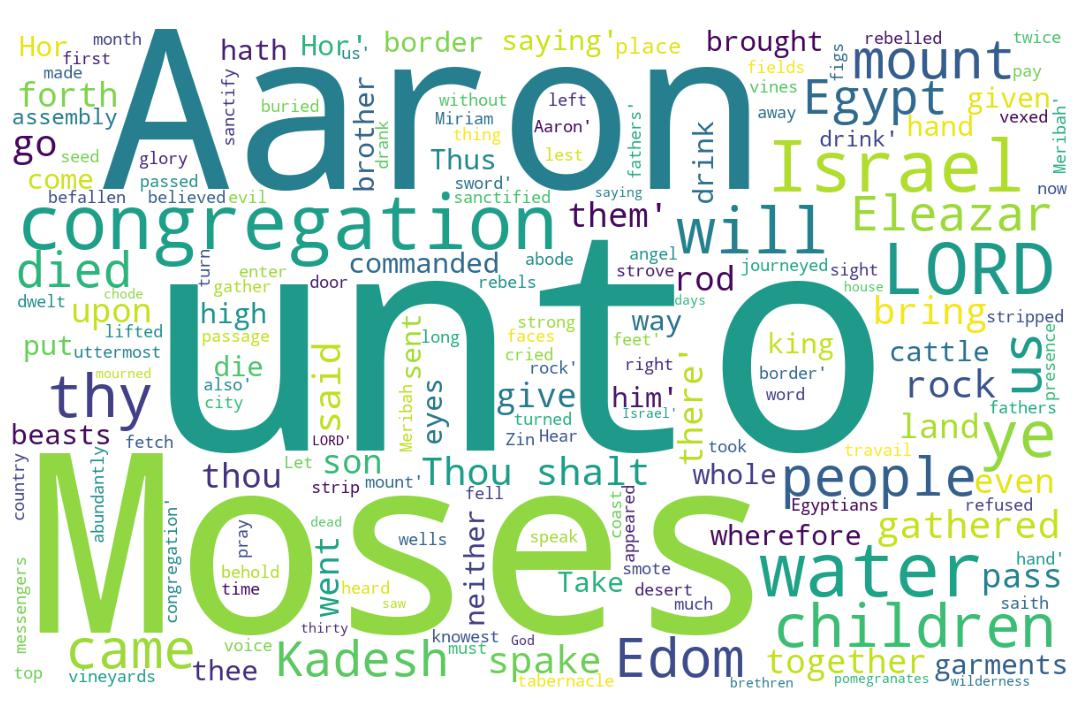
\includegraphics[width=\linewidth]{04OT-Numbers/Numbers20-WordCloud.jpg}
  \caption{Numbers 20 Word Cloud}
  \label{fig:Numbers 20 word Cloud}
\end{figure}

\marginpar{\scriptsize \centering \fcolorbox{bone}{lime}{\textbf{THE ROCK SMITTEN}}\\ (Numbers 20)
\begin{compactenum}[I.][8]
    \item  \textbf{Reaction} of Moses \index[scripture]{Numbers!Num 20:06} \index[scripture]{Numbers!Num 20:10}  (Numbers 20:6, 10)
    \item  \textbf{Rod} \index[scripture]{Numbers!Num 20:08} \index[scripture]{Numbers!Num 20:09}\index[scripture]{Numbers!Num 20:11} (Numbers 20:8, 9, 11)
    \item  \textbf{Rock} %\index[scripture]{Numbers!Num 20:11}  (Numbers 20:11) -- the typology of the third day and the seventh day
    \item  The \textbf{Rage} of Moses \index[scripture]{Numbers!Num 20:11}  (Numbers 20:11)
    \item  \textbf{Ruining} of a type \index[scripture]{Numbers!Num 20:11}  (Numbers 20:11)
    \item  \textbf{Rebels}  \index[scripture]{Numbers!Num 20:10} \index[scripture]{Numbers!Num 20:24} (Numbers 20:10, 24)
    \item  The \textbf{Revelation} -- the Law is unable to take God's people into the Promised Land %\index[scripture]{Numbers!Num 20:11}  (Numbers 20:11)
\end{compactenum}}
 
\footnote{\textcolor[rgb]{0.00,0.25,0.00}{\hyperlink{NumbersTOC}{Return to end of Table of Contents.}}}\footnote{\href{https://audiobible.com/bible/numbers_20.html}{\textcolor[cmyk]{0.99998,1,0,0}{Numbers 20 Audio}}}\textcolor[cmyk]{0.99998,1,0,0}{Then came the children of Israel, \emph{even} the whole congregation, into the desert of Zin in the first month: and the people abode in Kadesh; and Miriam died there, and was buried there.}
[2] \textcolor[cmyk]{0.99998,1,0,0}{And there was no water for the congregation: and they gathered themselves together against \fcolorbox{bone}{bone}{Moses} and against Aaron.}
[3] \textcolor[cmyk]{0.99998,1,0,0}{And the people chode with Moses, and spake, saying, Would God that we had died when our brethren died before the LORD!}
[4] \textcolor[cmyk]{0.99998,1,0,0}{And why have ye brought up the congregation of the LORD into this wilderness, that we and our cattle should die there?}
[5] \textcolor[cmyk]{0.99998,1,0,0}{And wherefore have ye made us to come up out of Egypt, to bring us in unto this evil place? it \emph{is} no place of seed, or of figs, or of vines, or of pomegranates; neither \emph{is} there any water to drink.}\
[6] \textcolor[cmyk]{0.99998,1,0,0}{And \fcolorbox{bone}{bone}{Moses} and Aaron went from the presence of the assembly unto the door of the tabernacle of the congregation, and they fell upon their faces: and the glory of the LORD appeared unto them.}\\
\\
\P \textcolor[cmyk]{0.99998,1,0,0}{And the LORD spake unto Moses, saying,}
[8] \textcolor[cmyk]{0.99998,1,0,0}{Take the rod, and gather thou the assembly together, thou, and Aaron thy brother, and speak ye unto the rock before their eyes; and it shall give forth his water, and thou shalt bring forth to them water out of the rock: so thou shalt give the congregation and their beasts drink.}
[9] \textcolor[cmyk]{0.99998,1,0,0}{And \fcolorbox{bone}{bone}{Moses} took the rod from before the LORD, as he commanded him.}
[10] \textcolor[cmyk]{0.99998,1,0,0}{And \fcolorbox{bone}{bone}{Moses} and Aaron gathered the congregation together before the rock, and he said unto them, Hear now, ye rebels; must we fetch you water out of this rock?}
[11] \textcolor[cmyk]{0.99998,1,0,0}{And \fcolorbox{bone}{bone}{Moses} lifted up his hand, and with his rod he smote the rock twice: and the water came out abundantly, and the congregation drank, and their beasts \emph{also}.}\\
\\
\P \textcolor[cmyk]{0.99998,1,0,0}{And the LORD spake unto \fcolorbox{bone}{bone}{Moses} and Aaron, Because ye believed me not, to sanctify me in the eyes of the children of Israel, therefore ye shall not bring this congregation into the land which I have given them.}
[13] \textcolor[cmyk]{0.99998,1,0,0}{This \emph{is} the water of Meribah; because the children of Israel strove with the LORD, and he was sanctified in them.}\\
\\
\P  \textcolor[cmyk]{0.99998,1,0,0}{And \fcolorbox{bone}{bone}{Moses} sent messengers from Kadesh unto the king of Edom, Thus saith thy brother Israel, Thou knowest all the travail that hath befallen us:}
[15] \textcolor[cmyk]{0.99998,1,0,0}{How our fathers went down into Egypt, and we have dwelt in Egypt a long time; and the Egyptians vexed us, and our fathers:}
[16] \textcolor[cmyk]{0.99998,1,0,0}{And when we cried unto the LORD, he heard our voice, and sent an angel, and hath brought us forth out of Egypt: and, behold, we \emph{are} in Kadesh, a city in the uttermost of thy border:}
[17] \textcolor[cmyk]{0.99998,1,0,0}{Let us pass, I pray thee, through thy country: we will not pass through the fields, or through the vineyards, neither will we drink \emph{of} the water of the wells: we will go by the king's \emph{high} way, we will not turn to the right hand nor to the left, until we have passed thy borders.}
[18] \textcolor[cmyk]{0.99998,1,0,0}{And Edom said unto him, Thou shalt not pass by me, lest I come out against thee with the sword.}
[19] \textcolor[cmyk]{0.99998,1,0,0}{And the children of Israel said unto him, We will go by the high way: and if I and my cattle drink of thy water, then I will pay for it: I will only, without \emph{doing} any thing \emph{else}, go through on my feet.}
[20] \textcolor[cmyk]{0.99998,1,0,0}{And he said, Thou shalt not go through. And Edom came out against him with much people, and with a strong hand.}
[21] \textcolor[cmyk]{0.99998,1,0,0}{Thus Edom refused to give Israel passage through his border: wherefore Israel turned away from him.}\\
\\
\P \textcolor[cmyk]{0.99998,1,0,0}{And the children of Israel, \emph{even} the whole congregation, journeyed from Kadesh, and came unto mount Hor.}
[23] \textcolor[cmyk]{0.99998,1,0,0}{And the LORD spake unto \fcolorbox{bone}{bone}{Moses} and Aaron in mount Hor, by the coast of the land of Edom, saying,}
[24] \textcolor[cmyk]{0.99998,1,0,0}{Aaron shall be gathered unto his people: for he shall not enter into the land which I have given unto the children of Israel, because ye rebelled against my word at the water of Meribah.}
[25] \textcolor[cmyk]{0.99998,1,0,0}{Take Aaron and Eleazar his son, and bring them up unto mount Hor:}
[26] \textcolor[cmyk]{0.99998,1,0,0}{And strip Aaron of his garments, and put them upon Eleazar his son: and Aaron shall be gathered \emph{unto} \emph{his} \emph{people}, and shall die there.}
[27] \textcolor[cmyk]{0.99998,1,0,0}{And \fcolorbox{bone}{bone}{Moses} did as the LORD commanded: and they went up into mount Hor in the sight of all the congregation.}
[28] \textcolor[cmyk]{0.99998,1,0,0}{And \fcolorbox{bone}{bone}{Moses} stripped Aaron of his garments, and put them upon Eleazar his son; and Aaron died there in the top of the mount: and \fcolorbox{bone}{bone}{Moses} and Eleazar came down from the mount.}
[29] \textcolor[cmyk]{0.99998,1,0,0}{And when all the congregation saw that Aaron was dead, they mourned for Aaron thirty days, \emph{even} all the house of Israel.}
\index[NWIV]{33!Numbers!Num 20:1}\index[AWIP]{Then!Numbers!Num 20:1}\index[AWIP]{came!Numbers!Num 20:1}\index[AWIP]{the!Numbers!Num 20:1}\index[AWIP]{the!Numbers!Num 20:1 (2)}\index[AWIP]{the!Numbers!Num 20:1 (3)}\index[AWIP]{the!Numbers!Num 20:1 (4)}\index[AWIP]{the!Numbers!Num 20:1 (5)}\index[AWIP]{children!Numbers!Num 20:1}\index[AWIP]{of!Numbers!Num 20:1}\index[AWIP]{of!Numbers!Num 20:1 (2)}\index[AWIP]{Israel!Numbers!Num 20:1}\index[AWIP]{\emph{even}!Numbers!Num 20:1}\index[AWIP]{whole!Numbers!Num 20:1}\index[AWIP]{congregation!Numbers!Num 20:1}\index[AWIP]{into!Numbers!Num 20:1}\index[AWIP]{desert!Numbers!Num 20:1}\index[AWIP]{Zin!Numbers!Num 20:1}\index[AWIP]{in!Numbers!Num 20:1}\index[AWIP]{in!Numbers!Num 20:1 (2)}\index[AWIP]{first!Numbers!Num 20:1}\index[AWIP]{month!Numbers!Num 20:1}\index[AWIP]{and!Numbers!Num 20:1}\index[AWIP]{and!Numbers!Num 20:1 (2)}\index[AWIP]{and!Numbers!Num 20:1 (3)}\index[AWIP]{people!Numbers!Num 20:1}\index[AWIP]{abode!Numbers!Num 20:1}\index[AWIP]{Kadesh!Numbers!Num 20:1}\index[AWIP]{Miriam!Numbers!Num 20:1}\index[AWIP]{died!Numbers!Num 20:1}\index[AWIP]{there!Numbers!Num 20:1}\index[AWIP]{there!Numbers!Num 20:1 (2)}\index[AWIP]{was!Numbers!Num 20:1}\index[AWIP]{buried!Numbers!Num 20:1}\index[AWIP]{\emph{even}!Numbers!Num 20:1}

\index[NWIV]{18!Numbers!Num 20:2}\index[AWIP]{And!Numbers!Num 20:2}\index[AWIP]{there!Numbers!Num 20:2}\index[AWIP]{was!Numbers!Num 20:2}\index[AWIP]{no!Numbers!Num 20:2}\index[AWIP]{water!Numbers!Num 20:2}\index[AWIP]{for!Numbers!Num 20:2}\index[AWIP]{the!Numbers!Num 20:2}\index[AWIP]{congregation!Numbers!Num 20:2}\index[AWIP]{and!Numbers!Num 20:2}\index[AWIP]{and!Numbers!Num 20:2 (2)}\index[AWIP]{they!Numbers!Num 20:2}\index[AWIP]{gathered!Numbers!Num 20:2}\index[AWIP]{themselves!Numbers!Num 20:2}\index[AWIP]{together!Numbers!Num 20:2}\index[AWIP]{against!Numbers!Num 20:2}\index[AWIP]{against!Numbers!Num 20:2 (2)}\index[AWIP]{Moses!Numbers!Num 20:2}\index[AWIP]{Aaron!Numbers!Num 20:2}

\index[NWIV]{22!Numbers!Num 20:3}\index[AWIP]{And!Numbers!Num 20:3}\index[AWIP]{the!Numbers!Num 20:3}\index[AWIP]{the!Numbers!Num 20:3 (2)}\index[AWIP]{people!Numbers!Num 20:3}\index[AWIP]{chode!Numbers!Num 20:3}\index[AWIP]{with!Numbers!Num 20:3}\index[AWIP]{Moses!Numbers!Num 20:3}\index[AWIP]{and!Numbers!Num 20:3}\index[AWIP]{spake!Numbers!Num 20:3}\index[AWIP]{saying!Numbers!Num 20:3}\index[AWIP]{Would!Numbers!Num 20:3}\index[AWIP]{God!Numbers!Num 20:3}\index[AWIP]{that!Numbers!Num 20:3}\index[AWIP]{we!Numbers!Num 20:3}\index[AWIP]{had!Numbers!Num 20:3}\index[AWIP]{died!Numbers!Num 20:3}\index[AWIP]{died!Numbers!Num 20:3 (2)}\index[AWIP]{when!Numbers!Num 20:3}\index[AWIP]{our!Numbers!Num 20:3}\index[AWIP]{brethren!Numbers!Num 20:3}\index[AWIP]{before!Numbers!Num 20:3}\index[AWIP]{LORD!!Numbers!Num 20:3}

\index[NWIV]{22!Numbers!Num 20:4}\index[AWIP]{And!Numbers!Num 20:4}\index[AWIP]{why!Numbers!Num 20:4}\index[AWIP]{have!Numbers!Num 20:4}\index[AWIP]{ye!Numbers!Num 20:4}\index[AWIP]{brought!Numbers!Num 20:4}\index[AWIP]{up!Numbers!Num 20:4}\index[AWIP]{the!Numbers!Num 20:4}\index[AWIP]{the!Numbers!Num 20:4 (2)}\index[AWIP]{congregation!Numbers!Num 20:4}\index[AWIP]{of!Numbers!Num 20:4}\index[AWIP]{LORD!Numbers!Num 20:4}\index[AWIP]{into!Numbers!Num 20:4}\index[AWIP]{this!Numbers!Num 20:4}\index[AWIP]{wilderness!Numbers!Num 20:4}\index[AWIP]{that!Numbers!Num 20:4}\index[AWIP]{we!Numbers!Num 20:4}\index[AWIP]{and!Numbers!Num 20:4}\index[AWIP]{our!Numbers!Num 20:4}\index[AWIP]{cattle!Numbers!Num 20:4}\index[AWIP]{should!Numbers!Num 20:4}\index[AWIP]{die!Numbers!Num 20:4}\index[AWIP]{there?!Numbers!Num 20:4}

\index[NWIV]{42!Numbers!Num 20:5}\index[AWIP]{And!Numbers!Num 20:5}\index[AWIP]{wherefore!Numbers!Num 20:5}\index[AWIP]{have!Numbers!Num 20:5}\index[AWIP]{ye!Numbers!Num 20:5}\index[AWIP]{made!Numbers!Num 20:5}\index[AWIP]{us!Numbers!Num 20:5}\index[AWIP]{us!Numbers!Num 20:5 (2)}\index[AWIP]{to!Numbers!Num 20:5}\index[AWIP]{to!Numbers!Num 20:5 (2)}\index[AWIP]{to!Numbers!Num 20:5 (3)}\index[AWIP]{come!Numbers!Num 20:5}\index[AWIP]{up!Numbers!Num 20:5}\index[AWIP]{out!Numbers!Num 20:5}\index[AWIP]{of!Numbers!Num 20:5}\index[AWIP]{of!Numbers!Num 20:5 (2)}\index[AWIP]{of!Numbers!Num 20:5 (3)}\index[AWIP]{of!Numbers!Num 20:5 (4)}\index[AWIP]{of!Numbers!Num 20:5 (5)}\index[AWIP]{Egypt!Numbers!Num 20:5}\index[AWIP]{bring!Numbers!Num 20:5}\index[AWIP]{in!Numbers!Num 20:5}\index[AWIP]{unto!Numbers!Num 20:5}\index[AWIP]{this!Numbers!Num 20:5}\index[AWIP]{evil!Numbers!Num 20:5}\index[AWIP]{place?!Numbers!Num 20:5}\index[AWIP]{it!Numbers!Num 20:5}\index[AWIP]{\emph{is}!Numbers!Num 20:5}\index[AWIP]{\emph{is}!Numbers!Num 20:5 (2)}\index[AWIP]{no!Numbers!Num 20:5}\index[AWIP]{place!Numbers!Num 20:5}\index[AWIP]{seed!Numbers!Num 20:5}\index[AWIP]{or!Numbers!Num 20:5}\index[AWIP]{or!Numbers!Num 20:5 (2)}\index[AWIP]{or!Numbers!Num 20:5 (3)}\index[AWIP]{figs!Numbers!Num 20:5}\index[AWIP]{vines!Numbers!Num 20:5}\index[AWIP]{pomegranates!Numbers!Num 20:5}\index[AWIP]{neither!Numbers!Num 20:5}\index[AWIP]{there!Numbers!Num 20:5}\index[AWIP]{any!Numbers!Num 20:5}\index[AWIP]{water!Numbers!Num 20:5}\index[AWIP]{drink!Numbers!Num 20:5}\index[AWIP]{\emph{is}!Numbers!Num 20:5}\index[AWIP]{\emph{is}!Numbers!Num 20:5 (2)}

\index[NWIV]{35!Numbers!Num 20:6}\index[AWIP]{And!Numbers!Num 20:6}\index[AWIP]{Moses!Numbers!Num 20:6}\index[AWIP]{and!Numbers!Num 20:6}\index[AWIP]{and!Numbers!Num 20:6 (2)}\index[AWIP]{and!Numbers!Num 20:6 (3)}\index[AWIP]{Aaron!Numbers!Num 20:6}\index[AWIP]{went!Numbers!Num 20:6}\index[AWIP]{from!Numbers!Num 20:6}\index[AWIP]{the!Numbers!Num 20:6}\index[AWIP]{the!Numbers!Num 20:6 (2)}\index[AWIP]{the!Numbers!Num 20:6 (3)}\index[AWIP]{the!Numbers!Num 20:6 (4)}\index[AWIP]{the!Numbers!Num 20:6 (5)}\index[AWIP]{the!Numbers!Num 20:6 (6)}\index[AWIP]{the!Numbers!Num 20:6 (7)}\index[AWIP]{presence!Numbers!Num 20:6}\index[AWIP]{of!Numbers!Num 20:6}\index[AWIP]{of!Numbers!Num 20:6 (2)}\index[AWIP]{of!Numbers!Num 20:6 (3)}\index[AWIP]{of!Numbers!Num 20:6 (4)}\index[AWIP]{assembly!Numbers!Num 20:6}\index[AWIP]{unto!Numbers!Num 20:6}\index[AWIP]{unto!Numbers!Num 20:6 (2)}\index[AWIP]{door!Numbers!Num 20:6}\index[AWIP]{tabernacle!Numbers!Num 20:6}\index[AWIP]{congregation!Numbers!Num 20:6}\index[AWIP]{they!Numbers!Num 20:6}\index[AWIP]{fell!Numbers!Num 20:6}\index[AWIP]{upon!Numbers!Num 20:6}\index[AWIP]{their!Numbers!Num 20:6}\index[AWIP]{faces!Numbers!Num 20:6}\index[AWIP]{glory!Numbers!Num 20:6}\index[AWIP]{LORD!Numbers!Num 20:6}\index[AWIP]{appeared!Numbers!Num 20:6}\index[AWIP]{them!Numbers!Num 20:6}

\index[NWIV]{7!Numbers!Num 20:7}\index[AWIP]{And!Numbers!Num 20:7}\index[AWIP]{the!Numbers!Num 20:7}\index[AWIP]{LORD!Numbers!Num 20:7}\index[AWIP]{spake!Numbers!Num 20:7}\index[AWIP]{unto!Numbers!Num 20:7}\index[AWIP]{Moses!Numbers!Num 20:7}\index[AWIP]{saying!Numbers!Num 20:7}

\index[NWIV]{52!Numbers!Num 20:8}\index[AWIP]{Take!Numbers!Num 20:8}\index[AWIP]{the!Numbers!Num 20:8}\index[AWIP]{the!Numbers!Num 20:8 (2)}\index[AWIP]{the!Numbers!Num 20:8 (3)}\index[AWIP]{the!Numbers!Num 20:8 (4)}\index[AWIP]{the!Numbers!Num 20:8 (5)}\index[AWIP]{rod!Numbers!Num 20:8}\index[AWIP]{and!Numbers!Num 20:8}\index[AWIP]{and!Numbers!Num 20:8 (2)}\index[AWIP]{and!Numbers!Num 20:8 (3)}\index[AWIP]{and!Numbers!Num 20:8 (4)}\index[AWIP]{and!Numbers!Num 20:8 (5)}\index[AWIP]{and!Numbers!Num 20:8 (6)}\index[AWIP]{gather!Numbers!Num 20:8}\index[AWIP]{thou!Numbers!Num 20:8}\index[AWIP]{thou!Numbers!Num 20:8 (2)}\index[AWIP]{thou!Numbers!Num 20:8 (3)}\index[AWIP]{thou!Numbers!Num 20:8 (4)}\index[AWIP]{assembly!Numbers!Num 20:8}\index[AWIP]{together!Numbers!Num 20:8}\index[AWIP]{Aaron!Numbers!Num 20:8}\index[AWIP]{thy!Numbers!Num 20:8}\index[AWIP]{brother!Numbers!Num 20:8}\index[AWIP]{speak!Numbers!Num 20:8}\index[AWIP]{ye!Numbers!Num 20:8}\index[AWIP]{unto!Numbers!Num 20:8}\index[AWIP]{rock!Numbers!Num 20:8}\index[AWIP]{rock!Numbers!Num 20:8 (2)}\index[AWIP]{before!Numbers!Num 20:8}\index[AWIP]{their!Numbers!Num 20:8}\index[AWIP]{their!Numbers!Num 20:8 (2)}\index[AWIP]{eyes!Numbers!Num 20:8}\index[AWIP]{it!Numbers!Num 20:8}\index[AWIP]{shall!Numbers!Num 20:8}\index[AWIP]{give!Numbers!Num 20:8}\index[AWIP]{give!Numbers!Num 20:8 (2)}\index[AWIP]{forth!Numbers!Num 20:8}\index[AWIP]{forth!Numbers!Num 20:8 (2)}\index[AWIP]{his!Numbers!Num 20:8}\index[AWIP]{water!Numbers!Num 20:8}\index[AWIP]{water!Numbers!Num 20:8 (2)}\index[AWIP]{shalt!Numbers!Num 20:8}\index[AWIP]{shalt!Numbers!Num 20:8 (2)}\index[AWIP]{bring!Numbers!Num 20:8}\index[AWIP]{to!Numbers!Num 20:8}\index[AWIP]{them!Numbers!Num 20:8}\index[AWIP]{out!Numbers!Num 20:8}\index[AWIP]{of!Numbers!Num 20:8}\index[AWIP]{so!Numbers!Num 20:8}\index[AWIP]{congregation!Numbers!Num 20:8}\index[AWIP]{beasts!Numbers!Num 20:8}\index[AWIP]{drink!Numbers!Num 20:8}

\index[NWIV]{13!Numbers!Num 20:9}\index[AWIP]{And!Numbers!Num 20:9}\index[AWIP]{Moses!Numbers!Num 20:9}\index[AWIP]{took!Numbers!Num 20:9}\index[AWIP]{the!Numbers!Num 20:9}\index[AWIP]{the!Numbers!Num 20:9 (2)}\index[AWIP]{rod!Numbers!Num 20:9}\index[AWIP]{from!Numbers!Num 20:9}\index[AWIP]{before!Numbers!Num 20:9}\index[AWIP]{LORD!Numbers!Num 20:9}\index[AWIP]{as!Numbers!Num 20:9}\index[AWIP]{he!Numbers!Num 20:9}\index[AWIP]{commanded!Numbers!Num 20:9}\index[AWIP]{him!Numbers!Num 20:9}

\index[NWIV]{29!Numbers!Num 20:10}\index[AWIP]{And!Numbers!Num 20:10}\index[AWIP]{Moses!Numbers!Num 20:10}\index[AWIP]{and!Numbers!Num 20:10}\index[AWIP]{and!Numbers!Num 20:10 (2)}\index[AWIP]{Aaron!Numbers!Num 20:10}\index[AWIP]{gathered!Numbers!Num 20:10}\index[AWIP]{the!Numbers!Num 20:10}\index[AWIP]{the!Numbers!Num 20:10 (2)}\index[AWIP]{congregation!Numbers!Num 20:10}\index[AWIP]{together!Numbers!Num 20:10}\index[AWIP]{before!Numbers!Num 20:10}\index[AWIP]{rock!Numbers!Num 20:10}\index[AWIP]{he!Numbers!Num 20:10}\index[AWIP]{said!Numbers!Num 20:10}\index[AWIP]{unto!Numbers!Num 20:10}\index[AWIP]{them!Numbers!Num 20:10}\index[AWIP]{Hear!Numbers!Num 20:10}\index[AWIP]{now!Numbers!Num 20:10}\index[AWIP]{ye!Numbers!Num 20:10}\index[AWIP]{rebels!Numbers!Num 20:10}\index[AWIP]{must!Numbers!Num 20:10}\index[AWIP]{we!Numbers!Num 20:10}\index[AWIP]{fetch!Numbers!Num 20:10}\index[AWIP]{you!Numbers!Num 20:10}\index[AWIP]{water!Numbers!Num 20:10}\index[AWIP]{out!Numbers!Num 20:10}\index[AWIP]{of!Numbers!Num 20:10}\index[AWIP]{this!Numbers!Num 20:10}\index[AWIP]{rock?!Numbers!Num 20:10}

\index[NWIV]{29!Numbers!Num 20:11}\index[AWIP]{And!Numbers!Num 20:11}\index[AWIP]{Moses!Numbers!Num 20:11}\index[AWIP]{lifted!Numbers!Num 20:11}\index[AWIP]{up!Numbers!Num 20:11}\index[AWIP]{his!Numbers!Num 20:11}\index[AWIP]{his!Numbers!Num 20:11 (2)}\index[AWIP]{hand!Numbers!Num 20:11}\index[AWIP]{and!Numbers!Num 20:11}\index[AWIP]{and!Numbers!Num 20:11 (2)}\index[AWIP]{and!Numbers!Num 20:11 (3)}\index[AWIP]{and!Numbers!Num 20:11 (4)}\index[AWIP]{with!Numbers!Num 20:11}\index[AWIP]{rod!Numbers!Num 20:11}\index[AWIP]{he!Numbers!Num 20:11}\index[AWIP]{smote!Numbers!Num 20:11}\index[AWIP]{the!Numbers!Num 20:11}\index[AWIP]{the!Numbers!Num 20:11 (2)}\index[AWIP]{the!Numbers!Num 20:11 (3)}\index[AWIP]{rock!Numbers!Num 20:11}\index[AWIP]{twice!Numbers!Num 20:11}\index[AWIP]{water!Numbers!Num 20:11}\index[AWIP]{came!Numbers!Num 20:11}\index[AWIP]{out!Numbers!Num 20:11}\index[AWIP]{abundantly!Numbers!Num 20:11}\index[AWIP]{congregation!Numbers!Num 20:11}\index[AWIP]{drank!Numbers!Num 20:11}\index[AWIP]{their!Numbers!Num 20:11}\index[AWIP]{beasts!Numbers!Num 20:11}\index[AWIP]{\emph{also}!Numbers!Num 20:11}\index[AWIP]{\emph{also}!Numbers!Num 20:11}

\index[NWIV]{39!Numbers!Num 20:12}\index[AWIP]{And!Numbers!Num 20:12}\index[AWIP]{the!Numbers!Num 20:12}\index[AWIP]{the!Numbers!Num 20:12 (2)}\index[AWIP]{the!Numbers!Num 20:12 (3)}\index[AWIP]{the!Numbers!Num 20:12 (4)}\index[AWIP]{LORD!Numbers!Num 20:12}\index[AWIP]{spake!Numbers!Num 20:12}\index[AWIP]{unto!Numbers!Num 20:12}\index[AWIP]{Moses!Numbers!Num 20:12}\index[AWIP]{and!Numbers!Num 20:12}\index[AWIP]{Aaron!Numbers!Num 20:12}\index[AWIP]{Because!Numbers!Num 20:12}\index[AWIP]{ye!Numbers!Num 20:12}\index[AWIP]{ye!Numbers!Num 20:12 (2)}\index[AWIP]{believed!Numbers!Num 20:12}\index[AWIP]{me!Numbers!Num 20:12}\index[AWIP]{me!Numbers!Num 20:12 (2)}\index[AWIP]{not!Numbers!Num 20:12}\index[AWIP]{not!Numbers!Num 20:12 (2)}\index[AWIP]{to!Numbers!Num 20:12}\index[AWIP]{sanctify!Numbers!Num 20:12}\index[AWIP]{in!Numbers!Num 20:12}\index[AWIP]{eyes!Numbers!Num 20:12}\index[AWIP]{of!Numbers!Num 20:12}\index[AWIP]{of!Numbers!Num 20:12 (2)}\index[AWIP]{children!Numbers!Num 20:12}\index[AWIP]{Israel!Numbers!Num 20:12}\index[AWIP]{therefore!Numbers!Num 20:12}\index[AWIP]{shall!Numbers!Num 20:12}\index[AWIP]{bring!Numbers!Num 20:12}\index[AWIP]{this!Numbers!Num 20:12}\index[AWIP]{congregation!Numbers!Num 20:12}\index[AWIP]{into!Numbers!Num 20:12}\index[AWIP]{land!Numbers!Num 20:12}\index[AWIP]{which!Numbers!Num 20:12}\index[AWIP]{I!Numbers!Num 20:12}\index[AWIP]{have!Numbers!Num 20:12}\index[AWIP]{given!Numbers!Num 20:12}\index[AWIP]{them!Numbers!Num 20:12}

\index[NWIV]{21!Numbers!Num 20:13}\index[AWIP]{This!Numbers!Num 20:13}\index[AWIP]{\emph{is}!Numbers!Num 20:13}\index[AWIP]{the!Numbers!Num 20:13}\index[AWIP]{the!Numbers!Num 20:13 (2)}\index[AWIP]{the!Numbers!Num 20:13 (3)}\index[AWIP]{water!Numbers!Num 20:13}\index[AWIP]{of!Numbers!Num 20:13}\index[AWIP]{of!Numbers!Num 20:13 (2)}\index[AWIP]{Meribah!Numbers!Num 20:13}\index[AWIP]{because!Numbers!Num 20:13}\index[AWIP]{children!Numbers!Num 20:13}\index[AWIP]{Israel!Numbers!Num 20:13}\index[AWIP]{strove!Numbers!Num 20:13}\index[AWIP]{with!Numbers!Num 20:13}\index[AWIP]{LORD!Numbers!Num 20:13}\index[AWIP]{and!Numbers!Num 20:13}\index[AWIP]{he!Numbers!Num 20:13}\index[AWIP]{was!Numbers!Num 20:13}\index[AWIP]{sanctified!Numbers!Num 20:13}\index[AWIP]{in!Numbers!Num 20:13}\index[AWIP]{them!Numbers!Num 20:13}\index[AWIP]{\emph{is}!Numbers!Num 20:13}

\index[NWIV]{25!Numbers!Num 20:14}\index[AWIP]{And!Numbers!Num 20:14}\index[AWIP]{Moses!Numbers!Num 20:14}\index[AWIP]{sent!Numbers!Num 20:14}\index[AWIP]{messengers!Numbers!Num 20:14}\index[AWIP]{from!Numbers!Num 20:14}\index[AWIP]{Kadesh!Numbers!Num 20:14}\index[AWIP]{unto!Numbers!Num 20:14}\index[AWIP]{the!Numbers!Num 20:14}\index[AWIP]{the!Numbers!Num 20:14 (2)}\index[AWIP]{king!Numbers!Num 20:14}\index[AWIP]{of!Numbers!Num 20:14}\index[AWIP]{Edom!Numbers!Num 20:14}\index[AWIP]{Thus!Numbers!Num 20:14}\index[AWIP]{saith!Numbers!Num 20:14}\index[AWIP]{thy!Numbers!Num 20:14}\index[AWIP]{brother!Numbers!Num 20:14}\index[AWIP]{Israel!Numbers!Num 20:14}\index[AWIP]{Thou!Numbers!Num 20:14}\index[AWIP]{knowest!Numbers!Num 20:14}\index[AWIP]{all!Numbers!Num 20:14}\index[AWIP]{travail!Numbers!Num 20:14}\index[AWIP]{that!Numbers!Num 20:14}\index[AWIP]{hath!Numbers!Num 20:14}\index[AWIP]{befallen!Numbers!Num 20:14}\index[AWIP]{us!Numbers!Num 20:14}

\index[NWIV]{24!Numbers!Num 20:15}\index[AWIP]{How!Numbers!Num 20:15}\index[AWIP]{our!Numbers!Num 20:15}\index[AWIP]{our!Numbers!Num 20:15 (2)}\index[AWIP]{fathers!Numbers!Num 20:15}\index[AWIP]{fathers!Numbers!Num 20:15 (2)}\index[AWIP]{went!Numbers!Num 20:15}\index[AWIP]{down!Numbers!Num 20:15}\index[AWIP]{into!Numbers!Num 20:15}\index[AWIP]{Egypt!Numbers!Num 20:15}\index[AWIP]{Egypt!Numbers!Num 20:15 (2)}\index[AWIP]{and!Numbers!Num 20:15}\index[AWIP]{and!Numbers!Num 20:15 (2)}\index[AWIP]{and!Numbers!Num 20:15 (3)}\index[AWIP]{we!Numbers!Num 20:15}\index[AWIP]{have!Numbers!Num 20:15}\index[AWIP]{dwelt!Numbers!Num 20:15}\index[AWIP]{in!Numbers!Num 20:15}\index[AWIP]{a!Numbers!Num 20:15}\index[AWIP]{long!Numbers!Num 20:15}\index[AWIP]{time!Numbers!Num 20:15}\index[AWIP]{the!Numbers!Num 20:15}\index[AWIP]{Egyptians!Numbers!Num 20:15}\index[AWIP]{vexed!Numbers!Num 20:15}\index[AWIP]{us!Numbers!Num 20:15}

\index[NWIV]{37!Numbers!Num 20:16}\index[AWIP]{And!Numbers!Num 20:16}\index[AWIP]{when!Numbers!Num 20:16}\index[AWIP]{we!Numbers!Num 20:16}\index[AWIP]{we!Numbers!Num 20:16 (2)}\index[AWIP]{cried!Numbers!Num 20:16}\index[AWIP]{unto!Numbers!Num 20:16}\index[AWIP]{the!Numbers!Num 20:16}\index[AWIP]{the!Numbers!Num 20:16 (2)}\index[AWIP]{LORD!Numbers!Num 20:16}\index[AWIP]{he!Numbers!Num 20:16}\index[AWIP]{heard!Numbers!Num 20:16}\index[AWIP]{our!Numbers!Num 20:16}\index[AWIP]{voice!Numbers!Num 20:16}\index[AWIP]{and!Numbers!Num 20:16}\index[AWIP]{and!Numbers!Num 20:16 (2)}\index[AWIP]{and!Numbers!Num 20:16 (3)}\index[AWIP]{sent!Numbers!Num 20:16}\index[AWIP]{an!Numbers!Num 20:16}\index[AWIP]{angel!Numbers!Num 20:16}\index[AWIP]{hath!Numbers!Num 20:16}\index[AWIP]{brought!Numbers!Num 20:16}\index[AWIP]{us!Numbers!Num 20:16}\index[AWIP]{forth!Numbers!Num 20:16}\index[AWIP]{out!Numbers!Num 20:16}\index[AWIP]{of!Numbers!Num 20:16}\index[AWIP]{of!Numbers!Num 20:16 (2)}\index[AWIP]{Egypt!Numbers!Num 20:16}\index[AWIP]{behold!Numbers!Num 20:16}\index[AWIP]{\emph{are}!Numbers!Num 20:16}\index[AWIP]{in!Numbers!Num 20:16}\index[AWIP]{in!Numbers!Num 20:16 (2)}\index[AWIP]{Kadesh!Numbers!Num 20:16}\index[AWIP]{a!Numbers!Num 20:16}\index[AWIP]{city!Numbers!Num 20:16}\index[AWIP]{uttermost!Numbers!Num 20:16}\index[AWIP]{thy!Numbers!Num 20:16}\index[AWIP]{border!Numbers!Num 20:16}\index[AWIP]{\emph{are}!Numbers!Num 20:16}

\index[NWIV]{56!Numbers!Num 20:17}\index[AWIP]{Let!Numbers!Num 20:17}\index[AWIP]{us!Numbers!Num 20:17}\index[AWIP]{pass!Numbers!Num 20:17}\index[AWIP]{pass!Numbers!Num 20:17 (2)}\index[AWIP]{I!Numbers!Num 20:17}\index[AWIP]{pray!Numbers!Num 20:17}\index[AWIP]{thee!Numbers!Num 20:17}\index[AWIP]{through!Numbers!Num 20:17}\index[AWIP]{through!Numbers!Num 20:17 (2)}\index[AWIP]{through!Numbers!Num 20:17 (3)}\index[AWIP]{thy!Numbers!Num 20:17}\index[AWIP]{thy!Numbers!Num 20:17 (2)}\index[AWIP]{country!Numbers!Num 20:17}\index[AWIP]{we!Numbers!Num 20:17}\index[AWIP]{we!Numbers!Num 20:17 (2)}\index[AWIP]{we!Numbers!Num 20:17 (3)}\index[AWIP]{we!Numbers!Num 20:17 (4)}\index[AWIP]{we!Numbers!Num 20:17 (5)}\index[AWIP]{will!Numbers!Num 20:17}\index[AWIP]{will!Numbers!Num 20:17 (2)}\index[AWIP]{will!Numbers!Num 20:17 (3)}\index[AWIP]{will!Numbers!Num 20:17 (4)}\index[AWIP]{not!Numbers!Num 20:17}\index[AWIP]{not!Numbers!Num 20:17 (2)}\index[AWIP]{the!Numbers!Num 20:17}\index[AWIP]{the!Numbers!Num 20:17 (2)}\index[AWIP]{the!Numbers!Num 20:17 (3)}\index[AWIP]{the!Numbers!Num 20:17 (4)}\index[AWIP]{the!Numbers!Num 20:17 (5)}\index[AWIP]{the!Numbers!Num 20:17 (6)}\index[AWIP]{the!Numbers!Num 20:17 (7)}\index[AWIP]{fields!Numbers!Num 20:17}\index[AWIP]{or!Numbers!Num 20:17}\index[AWIP]{vineyards!Numbers!Num 20:17}\index[AWIP]{neither!Numbers!Num 20:17}\index[AWIP]{drink!Numbers!Num 20:17}\index[AWIP]{\emph{of}!Numbers!Num 20:17}\index[AWIP]{water!Numbers!Num 20:17}\index[AWIP]{of!Numbers!Num 20:17}\index[AWIP]{wells!Numbers!Num 20:17}\index[AWIP]{go!Numbers!Num 20:17}\index[AWIP]{by!Numbers!Num 20:17}\index[AWIP]{king's!Numbers!Num 20:17}\index[AWIP]{\emph{high}!Numbers!Num 20:17}\index[AWIP]{way!Numbers!Num 20:17}\index[AWIP]{turn!Numbers!Num 20:17}\index[AWIP]{to!Numbers!Num 20:17}\index[AWIP]{to!Numbers!Num 20:17 (2)}\index[AWIP]{right!Numbers!Num 20:17}\index[AWIP]{hand!Numbers!Num 20:17}\index[AWIP]{nor!Numbers!Num 20:17}\index[AWIP]{left!Numbers!Num 20:17}\index[AWIP]{until!Numbers!Num 20:17}\index[AWIP]{have!Numbers!Num 20:17}\index[AWIP]{passed!Numbers!Num 20:17}\index[AWIP]{borders!Numbers!Num 20:17}\index[AWIP]{\emph{of}!Numbers!Num 20:17}\index[AWIP]{\emph{high}!Numbers!Num 20:17}

\index[NWIV]{20!Numbers!Num 20:18}\index[AWIP]{And!Numbers!Num 20:18}\index[AWIP]{Edom!Numbers!Num 20:18}\index[AWIP]{said!Numbers!Num 20:18}\index[AWIP]{unto!Numbers!Num 20:18}\index[AWIP]{him!Numbers!Num 20:18}\index[AWIP]{Thou!Numbers!Num 20:18}\index[AWIP]{shalt!Numbers!Num 20:18}\index[AWIP]{not!Numbers!Num 20:18}\index[AWIP]{pass!Numbers!Num 20:18}\index[AWIP]{by!Numbers!Num 20:18}\index[AWIP]{me!Numbers!Num 20:18}\index[AWIP]{lest!Numbers!Num 20:18}\index[AWIP]{I!Numbers!Num 20:18}\index[AWIP]{come!Numbers!Num 20:18}\index[AWIP]{out!Numbers!Num 20:18}\index[AWIP]{against!Numbers!Num 20:18}\index[AWIP]{thee!Numbers!Num 20:18}\index[AWIP]{with!Numbers!Num 20:18}\index[AWIP]{the!Numbers!Num 20:18}\index[AWIP]{sword!Numbers!Num 20:18}

\index[NWIV]{44!Numbers!Num 20:19}\index[AWIP]{And!Numbers!Num 20:19}\index[AWIP]{the!Numbers!Num 20:19}\index[AWIP]{the!Numbers!Num 20:19 (2)}\index[AWIP]{children!Numbers!Num 20:19}\index[AWIP]{of!Numbers!Num 20:19}\index[AWIP]{of!Numbers!Num 20:19 (2)}\index[AWIP]{Israel!Numbers!Num 20:19}\index[AWIP]{said!Numbers!Num 20:19}\index[AWIP]{unto!Numbers!Num 20:19}\index[AWIP]{him!Numbers!Num 20:19}\index[AWIP]{We!Numbers!Num 20:19}\index[AWIP]{will!Numbers!Num 20:19}\index[AWIP]{will!Numbers!Num 20:19 (2)}\index[AWIP]{will!Numbers!Num 20:19 (3)}\index[AWIP]{go!Numbers!Num 20:19}\index[AWIP]{go!Numbers!Num 20:19 (2)}\index[AWIP]{by!Numbers!Num 20:19}\index[AWIP]{high!Numbers!Num 20:19}\index[AWIP]{way!Numbers!Num 20:19}\index[AWIP]{and!Numbers!Num 20:19}\index[AWIP]{and!Numbers!Num 20:19 (2)}\index[AWIP]{if!Numbers!Num 20:19}\index[AWIP]{I!Numbers!Num 20:19}\index[AWIP]{I!Numbers!Num 20:19 (2)}\index[AWIP]{I!Numbers!Num 20:19 (3)}\index[AWIP]{my!Numbers!Num 20:19}\index[AWIP]{my!Numbers!Num 20:19 (2)}\index[AWIP]{cattle!Numbers!Num 20:19}\index[AWIP]{drink!Numbers!Num 20:19}\index[AWIP]{thy!Numbers!Num 20:19}\index[AWIP]{water!Numbers!Num 20:19}\index[AWIP]{then!Numbers!Num 20:19}\index[AWIP]{pay!Numbers!Num 20:19}\index[AWIP]{for!Numbers!Num 20:19}\index[AWIP]{it!Numbers!Num 20:19}\index[AWIP]{only!Numbers!Num 20:19}\index[AWIP]{without!Numbers!Num 20:19}\index[AWIP]{\emph{doing}!Numbers!Num 20:19}\index[AWIP]{any!Numbers!Num 20:19}\index[AWIP]{thing!Numbers!Num 20:19}\index[AWIP]{\emph{else}!Numbers!Num 20:19}\index[AWIP]{through!Numbers!Num 20:19}\index[AWIP]{on!Numbers!Num 20:19}\index[AWIP]{feet!Numbers!Num 20:19}\index[AWIP]{\emph{doing}!Numbers!Num 20:19}\index[AWIP]{\emph{else}!Numbers!Num 20:19}

\index[NWIV]{22!Numbers!Num 20:20}\index[AWIP]{And!Numbers!Num 20:20}\index[AWIP]{And!Numbers!Num 20:20 (2)}\index[AWIP]{he!Numbers!Num 20:20}\index[AWIP]{said!Numbers!Num 20:20}\index[AWIP]{Thou!Numbers!Num 20:20}\index[AWIP]{shalt!Numbers!Num 20:20}\index[AWIP]{not!Numbers!Num 20:20}\index[AWIP]{go!Numbers!Num 20:20}\index[AWIP]{through!Numbers!Num 20:20}\index[AWIP]{Edom!Numbers!Num 20:20}\index[AWIP]{came!Numbers!Num 20:20}\index[AWIP]{out!Numbers!Num 20:20}\index[AWIP]{against!Numbers!Num 20:20}\index[AWIP]{him!Numbers!Num 20:20}\index[AWIP]{with!Numbers!Num 20:20}\index[AWIP]{with!Numbers!Num 20:20 (2)}\index[AWIP]{much!Numbers!Num 20:20}\index[AWIP]{people!Numbers!Num 20:20}\index[AWIP]{and!Numbers!Num 20:20}\index[AWIP]{a!Numbers!Num 20:20}\index[AWIP]{strong!Numbers!Num 20:20}\index[AWIP]{hand!Numbers!Num 20:20}

\index[NWIV]{16!Numbers!Num 20:21}\index[AWIP]{Thus!Numbers!Num 20:21}\index[AWIP]{Edom!Numbers!Num 20:21}\index[AWIP]{refused!Numbers!Num 20:21}\index[AWIP]{to!Numbers!Num 20:21}\index[AWIP]{give!Numbers!Num 20:21}\index[AWIP]{Israel!Numbers!Num 20:21}\index[AWIP]{Israel!Numbers!Num 20:21 (2)}\index[AWIP]{passage!Numbers!Num 20:21}\index[AWIP]{through!Numbers!Num 20:21}\index[AWIP]{his!Numbers!Num 20:21}\index[AWIP]{border!Numbers!Num 20:21}\index[AWIP]{wherefore!Numbers!Num 20:21}\index[AWIP]{turned!Numbers!Num 20:21}\index[AWIP]{away!Numbers!Num 20:21}\index[AWIP]{from!Numbers!Num 20:21}\index[AWIP]{him!Numbers!Num 20:21}

\index[NWIV]{17!Numbers!Num 20:22}\index[AWIP]{And!Numbers!Num 20:22}\index[AWIP]{the!Numbers!Num 20:22}\index[AWIP]{the!Numbers!Num 20:22 (2)}\index[AWIP]{children!Numbers!Num 20:22}\index[AWIP]{of!Numbers!Num 20:22}\index[AWIP]{Israel!Numbers!Num 20:22}\index[AWIP]{\emph{even}!Numbers!Num 20:22}\index[AWIP]{whole!Numbers!Num 20:22}\index[AWIP]{congregation!Numbers!Num 20:22}\index[AWIP]{journeyed!Numbers!Num 20:22}\index[AWIP]{from!Numbers!Num 20:22}\index[AWIP]{Kadesh!Numbers!Num 20:22}\index[AWIP]{and!Numbers!Num 20:22}\index[AWIP]{came!Numbers!Num 20:22}\index[AWIP]{unto!Numbers!Num 20:22}\index[AWIP]{mount!Numbers!Num 20:22}\index[AWIP]{Hor!Numbers!Num 20:22}\index[AWIP]{\emph{even}!Numbers!Num 20:22}

\index[NWIV]{20!Numbers!Num 20:23}\index[AWIP]{And!Numbers!Num 20:23}\index[AWIP]{the!Numbers!Num 20:23}\index[AWIP]{the!Numbers!Num 20:23 (2)}\index[AWIP]{the!Numbers!Num 20:23 (3)}\index[AWIP]{LORD!Numbers!Num 20:23}\index[AWIP]{spake!Numbers!Num 20:23}\index[AWIP]{unto!Numbers!Num 20:23}\index[AWIP]{Moses!Numbers!Num 20:23}\index[AWIP]{and!Numbers!Num 20:23}\index[AWIP]{Aaron!Numbers!Num 20:23}\index[AWIP]{in!Numbers!Num 20:23}\index[AWIP]{mount!Numbers!Num 20:23}\index[AWIP]{Hor!Numbers!Num 20:23}\index[AWIP]{by!Numbers!Num 20:23}\index[AWIP]{coast!Numbers!Num 20:23}\index[AWIP]{of!Numbers!Num 20:23}\index[AWIP]{of!Numbers!Num 20:23 (2)}\index[AWIP]{land!Numbers!Num 20:23}\index[AWIP]{Edom!Numbers!Num 20:23}\index[AWIP]{saying!Numbers!Num 20:23}

\index[NWIV]{35!Numbers!Num 20:24}\index[AWIP]{Aaron!Numbers!Num 20:24}\index[AWIP]{shall!Numbers!Num 20:24}\index[AWIP]{shall!Numbers!Num 20:24 (2)}\index[AWIP]{be!Numbers!Num 20:24}\index[AWIP]{gathered!Numbers!Num 20:24}\index[AWIP]{unto!Numbers!Num 20:24}\index[AWIP]{unto!Numbers!Num 20:24 (2)}\index[AWIP]{his!Numbers!Num 20:24}\index[AWIP]{people!Numbers!Num 20:24}\index[AWIP]{for!Numbers!Num 20:24}\index[AWIP]{he!Numbers!Num 20:24}\index[AWIP]{not!Numbers!Num 20:24}\index[AWIP]{enter!Numbers!Num 20:24}\index[AWIP]{into!Numbers!Num 20:24}\index[AWIP]{the!Numbers!Num 20:24}\index[AWIP]{the!Numbers!Num 20:24 (2)}\index[AWIP]{the!Numbers!Num 20:24 (3)}\index[AWIP]{land!Numbers!Num 20:24}\index[AWIP]{which!Numbers!Num 20:24}\index[AWIP]{I!Numbers!Num 20:24}\index[AWIP]{have!Numbers!Num 20:24}\index[AWIP]{given!Numbers!Num 20:24}\index[AWIP]{children!Numbers!Num 20:24}\index[AWIP]{of!Numbers!Num 20:24}\index[AWIP]{of!Numbers!Num 20:24 (2)}\index[AWIP]{Israel!Numbers!Num 20:24}\index[AWIP]{because!Numbers!Num 20:24}\index[AWIP]{ye!Numbers!Num 20:24}\index[AWIP]{rebelled!Numbers!Num 20:24}\index[AWIP]{against!Numbers!Num 20:24}\index[AWIP]{my!Numbers!Num 20:24}\index[AWIP]{word!Numbers!Num 20:24}\index[AWIP]{at!Numbers!Num 20:24}\index[AWIP]{water!Numbers!Num 20:24}\index[AWIP]{Meribah!Numbers!Num 20:24}

\index[NWIV]{13!Numbers!Num 20:25}\index[AWIP]{Take!Numbers!Num 20:25}\index[AWIP]{Aaron!Numbers!Num 20:25}\index[AWIP]{and!Numbers!Num 20:25}\index[AWIP]{and!Numbers!Num 20:25 (2)}\index[AWIP]{Eleazar!Numbers!Num 20:25}\index[AWIP]{his!Numbers!Num 20:25}\index[AWIP]{son!Numbers!Num 20:25}\index[AWIP]{bring!Numbers!Num 20:25}\index[AWIP]{them!Numbers!Num 20:25}\index[AWIP]{up!Numbers!Num 20:25}\index[AWIP]{unto!Numbers!Num 20:25}\index[AWIP]{mount!Numbers!Num 20:25}\index[AWIP]{Hor!Numbers!Num 20:25}

\index[NWIV]{25!Numbers!Num 20:26}\index[AWIP]{And!Numbers!Num 20:26}\index[AWIP]{strip!Numbers!Num 20:26}\index[AWIP]{Aaron!Numbers!Num 20:26}\index[AWIP]{Aaron!Numbers!Num 20:26 (2)}\index[AWIP]{of!Numbers!Num 20:26}\index[AWIP]{his!Numbers!Num 20:26}\index[AWIP]{his!Numbers!Num 20:26 (2)}\index[AWIP]{garments!Numbers!Num 20:26}\index[AWIP]{and!Numbers!Num 20:26}\index[AWIP]{and!Numbers!Num 20:26 (2)}\index[AWIP]{and!Numbers!Num 20:26 (3)}\index[AWIP]{put!Numbers!Num 20:26}\index[AWIP]{them!Numbers!Num 20:26}\index[AWIP]{upon!Numbers!Num 20:26}\index[AWIP]{Eleazar!Numbers!Num 20:26}\index[AWIP]{son!Numbers!Num 20:26}\index[AWIP]{shall!Numbers!Num 20:26}\index[AWIP]{shall!Numbers!Num 20:26 (2)}\index[AWIP]{be!Numbers!Num 20:26}\index[AWIP]{gathered!Numbers!Num 20:26}\index[AWIP]{\emph{unto}!Numbers!Num 20:26}\index[AWIP]{\emph{his}!Numbers!Num 20:26}\index[AWIP]{\emph{people}!Numbers!Num 20:26}\index[AWIP]{die!Numbers!Num 20:26}\index[AWIP]{there!Numbers!Num 20:26}\index[AWIP]{\emph{unto}!Numbers!Num 20:26}\index[AWIP]{\emph{his}!Numbers!Num 20:26}\index[AWIP]{\emph{people}!Numbers!Num 20:26}

\index[NWIV]{21!Numbers!Num 20:27}\index[AWIP]{And!Numbers!Num 20:27}\index[AWIP]{Moses!Numbers!Num 20:27}\index[AWIP]{did!Numbers!Num 20:27}\index[AWIP]{as!Numbers!Num 20:27}\index[AWIP]{the!Numbers!Num 20:27}\index[AWIP]{the!Numbers!Num 20:27 (2)}\index[AWIP]{the!Numbers!Num 20:27 (3)}\index[AWIP]{LORD!Numbers!Num 20:27}\index[AWIP]{commanded!Numbers!Num 20:27}\index[AWIP]{and!Numbers!Num 20:27}\index[AWIP]{they!Numbers!Num 20:27}\index[AWIP]{went!Numbers!Num 20:27}\index[AWIP]{up!Numbers!Num 20:27}\index[AWIP]{into!Numbers!Num 20:27}\index[AWIP]{mount!Numbers!Num 20:27}\index[AWIP]{Hor!Numbers!Num 20:27}\index[AWIP]{in!Numbers!Num 20:27}\index[AWIP]{sight!Numbers!Num 20:27}\index[AWIP]{of!Numbers!Num 20:27}\index[AWIP]{all!Numbers!Num 20:27}\index[AWIP]{congregation!Numbers!Num 20:27}

\index[NWIV]{33!Numbers!Num 20:28}\index[AWIP]{And!Numbers!Num 20:28}\index[AWIP]{Moses!Numbers!Num 20:28}\index[AWIP]{Moses!Numbers!Num 20:28 (2)}\index[AWIP]{stripped!Numbers!Num 20:28}\index[AWIP]{Aaron!Numbers!Num 20:28}\index[AWIP]{Aaron!Numbers!Num 20:28 (2)}\index[AWIP]{of!Numbers!Num 20:28}\index[AWIP]{of!Numbers!Num 20:28 (2)}\index[AWIP]{his!Numbers!Num 20:28}\index[AWIP]{his!Numbers!Num 20:28 (2)}\index[AWIP]{garments!Numbers!Num 20:28}\index[AWIP]{and!Numbers!Num 20:28}\index[AWIP]{and!Numbers!Num 20:28 (2)}\index[AWIP]{and!Numbers!Num 20:28 (3)}\index[AWIP]{and!Numbers!Num 20:28 (4)}\index[AWIP]{put!Numbers!Num 20:28}\index[AWIP]{them!Numbers!Num 20:28}\index[AWIP]{upon!Numbers!Num 20:28}\index[AWIP]{Eleazar!Numbers!Num 20:28}\index[AWIP]{Eleazar!Numbers!Num 20:28 (2)}\index[AWIP]{son!Numbers!Num 20:28}\index[AWIP]{died!Numbers!Num 20:28}\index[AWIP]{there!Numbers!Num 20:28}\index[AWIP]{in!Numbers!Num 20:28}\index[AWIP]{the!Numbers!Num 20:28}\index[AWIP]{the!Numbers!Num 20:28 (2)}\index[AWIP]{the!Numbers!Num 20:28 (3)}\index[AWIP]{top!Numbers!Num 20:28}\index[AWIP]{mount!Numbers!Num 20:28}\index[AWIP]{mount!Numbers!Num 20:28 (2)}\index[AWIP]{came!Numbers!Num 20:28}\index[AWIP]{down!Numbers!Num 20:28}\index[AWIP]{from!Numbers!Num 20:28}

\index[NWIV]{22!Numbers!Num 20:29}\index[AWIP]{And!Numbers!Num 20:29}\index[AWIP]{when!Numbers!Num 20:29}\index[AWIP]{all!Numbers!Num 20:29}\index[AWIP]{all!Numbers!Num 20:29 (2)}\index[AWIP]{the!Numbers!Num 20:29}\index[AWIP]{the!Numbers!Num 20:29 (2)}\index[AWIP]{congregation!Numbers!Num 20:29}\index[AWIP]{saw!Numbers!Num 20:29}\index[AWIP]{that!Numbers!Num 20:29}\index[AWIP]{Aaron!Numbers!Num 20:29}\index[AWIP]{Aaron!Numbers!Num 20:29 (2)}\index[AWIP]{was!Numbers!Num 20:29}\index[AWIP]{dead!Numbers!Num 20:29}\index[AWIP]{they!Numbers!Num 20:29}\index[AWIP]{mourned!Numbers!Num 20:29}\index[AWIP]{for!Numbers!Num 20:29}\index[AWIP]{thirty!Numbers!Num 20:29}\index[AWIP]{days!Numbers!Num 20:29}\index[AWIP]{\emph{even}!Numbers!Num 20:29}\index[AWIP]{house!Numbers!Num 20:29}\index[AWIP]{of!Numbers!Num 20:29}\index[AWIP]{Israel!Numbers!Num 20:29}\index[AWIP]{\emph{even}!Numbers!Num 20:29}


\section{Number 20 Outlines}

\subsection{My Outlines}

\subsubsection{The Rock Smitten}
%Practical Wisdom from Proverbs 6:\footnote{03 November 2014, Keith Anthony}
\index[speaker]{Keith Anthony!Numbers 20 (The Rock Smitten}
\index[series]{Numbers (Keith Anthony)!Numbers 20 (The Rock Smitten}
\index[date]{2018/02/17!Numbers 20 (The Rock Smitten (Keith Anthony)}

\begin{compactenum}[I.]
    \item  \textbf{Reaction} of Moses \index[scripture]{Numbers!Num 20:06} \index[scripture]{Numbers!Num 20:10}  (Numbers 20:6, 10)
    \item  \textbf{Rod} \index[scripture]{Numbers!Num 20:08} \index[scripture]{Numbers!Num 20:09}\index[scripture]{Numbers!Num 20:11} (Numbers 20:8, 9, 11)
    \item  \textbf{Rock} %\index[scripture]{Numbers!Num 20:11}  (Numbers 20:11) -- the typology of the third day and the seventh day
    \item  The \textbf{Rage} of Moses \index[scripture]{Numbers!Num 20:11}  (Numbers 20:11)
    \item  \textbf{Ruining} of a type \index[scripture]{Numbers!Num 20:11}  (Numbers 20:11)
    \item  \textbf{Rebels}  \index[scripture]{Numbers!Num 20:10} \index[scripture]{Numbers!Num 20:24} (Numbers 20:10, 24)
    \item  The \textbf{Revelation} -- the Law is unable to take God's people into the Promised Land %\index[scripture]{Numbers!Num 20:11}  (Numbers 20:11)
\end{compactenum}




\subsection{Outlines from Others}
\section{Numbers 20 Comments}

\subsection{Numeric Nuggets}
\textbf{13: } Verses 9 and 25 have 13 words. The name ``Moses'' is used 13 times in the chapter.
\subsection{Numbers 20 Repeated Phrases}


%%%%%%%%%%
%%%%%%%%%%
\normalsize
 
\begin{center}
\begin{longtable}{|c|c|}
\caption[Numbers 20 Repeated Phrases]{Numbers 20 Repeated Phrases}\label{table:Repeated Phrases Numbers 20} \\
\hline \multicolumn{1}{|c|}{\textbf{Phrase}} & \multicolumn{1}{c|}{\textbf{Frequency}} \\ \hline 
\endfirsthead
 
\multicolumn{2}{c}
{{\bfseries \tablename\ \thetable{} -- continued from previous page}} \\  
\hline \multicolumn{1}{|c|}{\textbf{Phrase}} & \multicolumn{1}{c|}{\textbf{Frequency}} \\ \hline 
\endhead
 
\hline \multicolumn{2}{c}{{ }} \\ \hline
\endfoot 
the LORD & 10\\ \hline 
of the & 10\\ \hline 
the congregation & 8\\ \hline 
of Israel & 7\\ \hline 
Moses and & 7\\ \hline 
And Moses & 7\\ \hline 
and Aaron & 7\\ \hline 
the children & 6\\ \hline 
the children of & 6\\ \hline 
the children of Israel & 6\\ \hline 
children of & 6\\ \hline 
children of Israel & 6\\ \hline 
And the & 6\\ \hline 
in the & 5\\ \hline 
and the & 5\\ \hline 
unto the & 5\\ \hline 
out of & 4\\ \hline 
Moses and Aaron & 4\\ \hline 
the rock & 4\\ \hline 
the water & 4\\ \hline 
all the & 4\\ \hline 
mount Hor & 4\\ \hline 
into the & 3\\ \hline 
the congregation and & 3\\ \hline 
congregation and & 3\\ \hline 
and they & 3\\ \hline 
before the & 3\\ \hline 
or of & 3\\ \hline 
And the LORD & 3\\ \hline 
And the LORD spake & 3\\ \hline 
And the LORD spake unto & 3\\ \hline 
And the LORD spake unto Moses & 3\\ \hline 
the LORD spake & 3\\ \hline 
the LORD spake unto & 3\\ \hline 
the LORD spake unto Moses & 3\\ \hline 
LORD spake & 3\\ \hline 
LORD spake unto & 3\\ \hline 
LORD spake unto Moses & 3\\ \hline 
spake unto & 3\\ \hline 
spake unto Moses & 3\\ \hline 
unto Moses & 3\\ \hline 
said unto & 3\\ \hline 
the land & 3\\ \hline 
the water of & 3\\ \hline 
water of & 3\\ \hline 
we will & 3\\ \hline 
by the & 3\\ \hline 
Eleazar his & 3\\ \hline 
Eleazar his son & 3\\ \hline 
Eleazar his son and & 3\\ \hline 
his son & 3\\ \hline 
his son and & 3\\ \hline 
son and & 3\\ \hline 
\end{longtable}
\end{center}



%%%%%%%%%%
%%%%%%%%%%



\section{Numbers 20 Statistics}


%%%%%%%%%%%%%%%%%%%%%%%%%%%
%%%%% Word Statistics
%%%%%%%%%%%%%%%%%%%%%%%%%%


\normalsize



\subsection{Chapter Word Statistics}


%%%%%%%%%%
%%%%%%%%%%
 
\begin{center}
\begin{longtable}{l|c|c|c|c}
\caption[Stats for Numbers 20]{Stats for Numbers 20} \label{table:Stats for Numbers 20} \\ 
\hline \multicolumn{1}{|c|}{\textbf{Verse(s)}} & \multicolumn{1}{|c|}{\textbf{Count}} & \multicolumn{1}{|c|}{\textbf{Unique}} & \multicolumn{1}{|c|}{\textbf{Italics}} & \multicolumn{1}{|c|}{\textbf{Uniq Italic}}  \\ \hline 
\endfirsthead
 
\multicolumn{5}{c}
{{\bfseries \tablename\ \thetable{} -- continued from previous page}} \\  
\hline \multicolumn{1}{|c|}{\textbf{Verse(s)}} & \multicolumn{1}{|c|}{\textbf{Count}} & \multicolumn{1}{|c|}{\textbf{Unique}} & \multicolumn{1}{|c|}{\textbf{Italics}} & \multicolumn{1}{|c|}{\textbf{Uniq Italic}}  \\ \hline 
\endhead
 
\hline \multicolumn{5}{|r|}{{Continued if needed}} \\ \hline
\endfoot 
1 & 33 & 24 & 1 & 1\\ \hline
2 & 18 & 16 & 0 & 0\\ \hline
3 & 22 & 20 & 0 & 0\\ \hline
4 & 22 & 21 & 0 & 0\\ \hline
5 & 42 & 31 & 2 & 1\\ \hline
6 & 35 & 23 & 0 & 0\\ \hline
7 & 7 & 7 & 0 & 0\\ \hline
8 & 52 & 34 & 0 & 0\\ \hline
9 & 13 & 12 & 0 & 0\\ \hline
10 & 29 & 26 & 0 & 0\\ \hline
11 & 29 & 23 & 1 & 1\\ \hline
12 & 39 & 32 & 0 & 0\\ \hline
13 & 21 & 18 & 1 & 1\\ \hline
14 & 25 & 24 & 0 & 0\\ \hline
15 & 24 & 19 & 0 & 0\\ \hline
16 & 37 & 31 & 1 & 1\\ \hline
17 & 56 & 37 & 2 & 2\\ \hline
18 & 20 & 20 & 0 & 0\\ \hline
19 & 44 & 35 & 2 & 2\\ \hline
20 & 22 & 20 & 0 & 0\\ \hline
21 & 16 & 15 & 0 & 0\\ \hline
22 & 17 & 16 & 1 & 1\\ \hline
23 & 20 & 17 & 0 & 0\\ \hline
24 & 35 & 30 & 0 & 0\\ \hline
25 & 13 & 12 & 0 & 0\\ \hline
26 & 25 & 20 & 3 & 3\\ \hline
27 & 21 & 19 & 0 & 0\\ \hline
28 & 33 & 22 & 0 & 0\\ \hline
29 & 22 & 19 & 1 & 1\\ \hline
\hline \hline
Total & 792 & 245 & 15 & 11



\end{longtable}
\end{center}

%%%%%%%%%%
%%%%%%%%%%
 
\subsection{Words by Frequency}

\begin{center}
\begin{longtable}{l|r}
\caption[Word Frequencies in Numbers 20]{Word Frequencies in Numbers 20} \label{table:WordsIn-Numbers-20} \\ 
\hline \multicolumn{1}{|c|}{\textbf{Word}} & \multicolumn{1}{c|}{\textbf{Frequency}} \\ \hline 
\endfirsthead
 
\multicolumn{2}{c}
{{\bfseries \tablename\ \thetable{} -- continued from previous page}} \\ 
\hline \multicolumn{1}{|c|}{\textbf{Word}} & \multicolumn{1}{c|}{\textbf{Frequency}} \\ \hline 
\endhead
 
\hline \multicolumn{2}{|r|}{{Continued if needed}} \\ \hline
\endfoot
 
\hline \hline
\endlastfoot
the & 68 \\ \hline
and & 45 \\ \hline
of & 34 \\ \hline
And & 22 \\ \hline
unto & 16 \\ \hline
Aaron & 14 \\ \hline
Moses & 13 \\ \hline
congregation & 11 \\ \hline
in & 11 \\ \hline
we & 11 \\ \hline
Israel & 10 \\ \hline
water & 10 \\ \hline
LORD & 10 \\ \hline
his & 10 \\ \hline
to & 8 \\ \hline
them & 8 \\ \hline
there & 7 \\ \hline
ye & 7 \\ \hline
out & 7 \\ \hline
he & 7 \\ \hline
not & 7 \\ \hline
I & 7 \\ \hline
will & 7 \\ \hline
children & 6 \\ \hline
into & 6 \\ \hline
with & 6 \\ \hline
have & 6 \\ \hline
us & 6 \\ \hline
from & 6 \\ \hline
thy & 6 \\ \hline
shall & 6 \\ \hline
through & 6 \\ \hline
mount & 6 \\ \hline
came & 5 \\ \hline
against & 5 \\ \hline
our & 5 \\ \hline
up & 5 \\ \hline
rock & 5 \\ \hline
him & 5 \\ \hline
Edom & 5 \\ \hline
people & 4 \\ \hline
Kadesh & 4 \\ \hline
died & 4 \\ \hline
was & 4 \\ \hline
for & 4 \\ \hline
they & 4 \\ \hline
gathered & 4 \\ \hline
spake & 4 \\ \hline
that & 4 \\ \hline
before & 4 \\ \hline
this & 4 \\ \hline
Egypt & 4 \\ \hline
bring & 4 \\ \hline
or & 4 \\ \hline
drink & 4 \\ \hline
their & 4 \\ \hline
thou & 4 \\ \hline
shalt & 4 \\ \hline
said & 4 \\ \hline
all & 4 \\ \hline
go & 4 \\ \hline
by & 4 \\ \hline
Hor & 4 \\ \hline
Eleazar & 4 \\ \hline
\emph{even} & 3 \\ \hline
together & 3 \\ \hline
saying & 3 \\ \hline
when & 3 \\ \hline
it & 3 \\ \hline
\emph{is} & 3 \\ \hline
went & 3 \\ \hline
upon & 3 \\ \hline
rod & 3 \\ \hline
give & 3 \\ \hline
forth & 3 \\ \hline
hand & 3 \\ \hline
me & 3 \\ \hline
land & 3 \\ \hline
Thou & 3 \\ \hline
a & 3 \\ \hline
pass & 3 \\ \hline
my & 3 \\ \hline
son & 3 \\ \hline
whole & 2 \\ \hline
no & 2 \\ \hline
brought & 2 \\ \hline
cattle & 2 \\ \hline
die & 2 \\ \hline
wherefore & 2 \\ \hline
come & 2 \\ \hline
place & 2 \\ \hline
neither & 2 \\ \hline
any & 2 \\ \hline
assembly & 2 \\ \hline
Take & 2 \\ \hline
brother & 2 \\ \hline
eyes & 2 \\ \hline
beasts & 2 \\ \hline
as & 2 \\ \hline
commanded & 2 \\ \hline
which & 2 \\ \hline
given & 2 \\ \hline
Meribah & 2 \\ \hline
because & 2 \\ \hline
sent & 2 \\ \hline
Thus & 2 \\ \hline
hath & 2 \\ \hline
fathers & 2 \\ \hline
down & 2 \\ \hline
border & 2 \\ \hline
thee & 2 \\ \hline
way & 2 \\ \hline
be & 2 \\ \hline
garments & 2 \\ \hline
put & 2 \\ \hline
Then & 1 \\ \hline
desert & 1 \\ \hline
Zin & 1 \\ \hline
first & 1 \\ \hline
month & 1 \\ \hline
abode & 1 \\ \hline
Miriam & 1 \\ \hline
buried & 1 \\ \hline
themselves & 1 \\ \hline
chode & 1 \\ \hline
Would & 1 \\ \hline
God & 1 \\ \hline
had & 1 \\ \hline
brethren & 1 \\ \hline
why & 1 \\ \hline
wilderness & 1 \\ \hline
should & 1 \\ \hline
made & 1 \\ \hline
evil & 1 \\ \hline
seed & 1 \\ \hline
figs & 1 \\ \hline
vines & 1 \\ \hline
pomegranates & 1 \\ \hline
presence & 1 \\ \hline
door & 1 \\ \hline
tabernacle & 1 \\ \hline
fell & 1 \\ \hline
faces & 1 \\ \hline
glory & 1 \\ \hline
appeared & 1 \\ \hline
gather & 1 \\ \hline
speak & 1 \\ \hline
so & 1 \\ \hline
took & 1 \\ \hline
Hear & 1 \\ \hline
now & 1 \\ \hline
rebels & 1 \\ \hline
must & 1 \\ \hline
fetch & 1 \\ \hline
you & 1 \\ \hline
lifted & 1 \\ \hline
smote & 1 \\ \hline
twice & 1 \\ \hline
abundantly & 1 \\ \hline
drank & 1 \\ \hline
\emph{also} & 1 \\ \hline
Because & 1 \\ \hline
believed & 1 \\ \hline
sanctify & 1 \\ \hline
therefore & 1 \\ \hline
This & 1 \\ \hline
strove & 1 \\ \hline
sanctified & 1 \\ \hline
messengers & 1 \\ \hline
king & 1 \\ \hline
saith & 1 \\ \hline
knowest & 1 \\ \hline
travail & 1 \\ \hline
befallen & 1 \\ \hline
How & 1 \\ \hline
dwelt & 1 \\ \hline
long & 1 \\ \hline
time & 1 \\ \hline
Egyptians & 1 \\ \hline
vexed & 1 \\ \hline
cried & 1 \\ \hline
heard & 1 \\ \hline
voice & 1 \\ \hline
an & 1 \\ \hline
angel & 1 \\ \hline
behold & 1 \\ \hline
\emph{are} & 1 \\ \hline
city & 1 \\ \hline
uttermost & 1 \\ \hline
Let & 1 \\ \hline
pray & 1 \\ \hline
country & 1 \\ \hline
fields & 1 \\ \hline
vineyards & 1 \\ \hline
\emph{of} & 1 \\ \hline
wells & 1 \\ \hline
king's & 1 \\ \hline
\emph{high} & 1 \\ \hline
turn & 1 \\ \hline
right & 1 \\ \hline
nor & 1 \\ \hline
left & 1 \\ \hline
until & 1 \\ \hline
passed & 1 \\ \hline
borders & 1 \\ \hline
lest & 1 \\ \hline
sword & 1 \\ \hline
We & 1 \\ \hline
high & 1 \\ \hline
if & 1 \\ \hline
then & 1 \\ \hline
pay & 1 \\ \hline
only & 1 \\ \hline
without & 1 \\ \hline
\emph{doing} & 1 \\ \hline
thing & 1 \\ \hline
\emph{else} & 1 \\ \hline
on & 1 \\ \hline
feet & 1 \\ \hline
much & 1 \\ \hline
strong & 1 \\ \hline
refused & 1 \\ \hline
passage & 1 \\ \hline
turned & 1 \\ \hline
away & 1 \\ \hline
journeyed & 1 \\ \hline
coast & 1 \\ \hline
enter & 1 \\ \hline
rebelled & 1 \\ \hline
word & 1 \\ \hline
at & 1 \\ \hline
strip & 1 \\ \hline
\emph{unto} & 1 \\ \hline
\emph{his} & 1 \\ \hline
\emph{people} & 1 \\ \hline
did & 1 \\ \hline
sight & 1 \\ \hline
stripped & 1 \\ \hline
top & 1 \\ \hline
saw & 1 \\ \hline
dead & 1 \\ \hline
mourned & 1 \\ \hline
thirty & 1 \\ \hline
days & 1 \\ \hline
house & 1 \\ \hline
\end{longtable}
\end{center}



\normalsize



\subsection{Words Alphabetically}

\begin{center}
\begin{longtable}{l|r}
\caption[Word Alphabetically in Numbers 20]{Word Alphabetically in Numbers 20} \label{table:WordsIn-Numbers-20} \\ 
\hline \multicolumn{1}{|c|}{\textbf{Word}} & \multicolumn{1}{c|}{\textbf{Frequency}} \\ \hline 
\endfirsthead
 
\multicolumn{2}{c}
{{\bfseries \tablename\ \thetable{} -- continued from previous page}} \\ 
\hline \multicolumn{1}{|c|}{\textbf{Word}} & \multicolumn{1}{c|}{\textbf{Frequency}} \\ \hline 
\endhead
 
\hline \multicolumn{2}{|r|}{{Continued if needed}} \\ \hline
\endfoot
 
\hline \hline
\endlastfoot
Aaron & 14 \\ \hline
And & 22 \\ \hline
Because & 1 \\ \hline
Edom & 5 \\ \hline
Egypt & 4 \\ \hline
Egyptians & 1 \\ \hline
Eleazar & 4 \\ \hline
God & 1 \\ \hline
Hear & 1 \\ \hline
Hor & 4 \\ \hline
How & 1 \\ \hline
I & 7 \\ \hline
Israel & 10 \\ \hline
Kadesh & 4 \\ \hline
LORD & 10 \\ \hline
Let & 1 \\ \hline
Meribah & 2 \\ \hline
Miriam & 1 \\ \hline
Moses & 13 \\ \hline
Take & 2 \\ \hline
Then & 1 \\ \hline
This & 1 \\ \hline
Thou & 3 \\ \hline
Thus & 2 \\ \hline
We & 1 \\ \hline
Would & 1 \\ \hline
Zin & 1 \\ \hline
\emph{also} & 1 \\ \hline
\emph{are} & 1 \\ \hline
\emph{doing} & 1 \\ \hline
\emph{else} & 1 \\ \hline
\emph{even} & 3 \\ \hline
\emph{high} & 1 \\ \hline
\emph{his} & 1 \\ \hline
\emph{is} & 3 \\ \hline
\emph{of} & 1 \\ \hline
\emph{people} & 1 \\ \hline
\emph{unto} & 1 \\ \hline
a & 3 \\ \hline
abode & 1 \\ \hline
abundantly & 1 \\ \hline
against & 5 \\ \hline
all & 4 \\ \hline
an & 1 \\ \hline
and & 45 \\ \hline
angel & 1 \\ \hline
any & 2 \\ \hline
appeared & 1 \\ \hline
as & 2 \\ \hline
assembly & 2 \\ \hline
at & 1 \\ \hline
away & 1 \\ \hline
be & 2 \\ \hline
beasts & 2 \\ \hline
because & 2 \\ \hline
befallen & 1 \\ \hline
before & 4 \\ \hline
behold & 1 \\ \hline
believed & 1 \\ \hline
border & 2 \\ \hline
borders & 1 \\ \hline
brethren & 1 \\ \hline
bring & 4 \\ \hline
brother & 2 \\ \hline
brought & 2 \\ \hline
buried & 1 \\ \hline
by & 4 \\ \hline
came & 5 \\ \hline
cattle & 2 \\ \hline
children & 6 \\ \hline
chode & 1 \\ \hline
city & 1 \\ \hline
coast & 1 \\ \hline
come & 2 \\ \hline
commanded & 2 \\ \hline
congregation & 11 \\ \hline
country & 1 \\ \hline
cried & 1 \\ \hline
days & 1 \\ \hline
dead & 1 \\ \hline
desert & 1 \\ \hline
did & 1 \\ \hline
die & 2 \\ \hline
died & 4 \\ \hline
door & 1 \\ \hline
down & 2 \\ \hline
drank & 1 \\ \hline
drink & 4 \\ \hline
dwelt & 1 \\ \hline
enter & 1 \\ \hline
evil & 1 \\ \hline
eyes & 2 \\ \hline
faces & 1 \\ \hline
fathers & 2 \\ \hline
feet & 1 \\ \hline
fell & 1 \\ \hline
fetch & 1 \\ \hline
fields & 1 \\ \hline
figs & 1 \\ \hline
first & 1 \\ \hline
for & 4 \\ \hline
forth & 3 \\ \hline
from & 6 \\ \hline
garments & 2 \\ \hline
gather & 1 \\ \hline
gathered & 4 \\ \hline
give & 3 \\ \hline
given & 2 \\ \hline
glory & 1 \\ \hline
go & 4 \\ \hline
had & 1 \\ \hline
hand & 3 \\ \hline
hath & 2 \\ \hline
have & 6 \\ \hline
he & 7 \\ \hline
heard & 1 \\ \hline
high & 1 \\ \hline
him & 5 \\ \hline
his & 10 \\ \hline
house & 1 \\ \hline
if & 1 \\ \hline
in & 11 \\ \hline
into & 6 \\ \hline
it & 3 \\ \hline
journeyed & 1 \\ \hline
king & 1 \\ \hline
king's & 1 \\ \hline
knowest & 1 \\ \hline
land & 3 \\ \hline
left & 1 \\ \hline
lest & 1 \\ \hline
lifted & 1 \\ \hline
long & 1 \\ \hline
made & 1 \\ \hline
me & 3 \\ \hline
messengers & 1 \\ \hline
month & 1 \\ \hline
mount & 6 \\ \hline
mourned & 1 \\ \hline
much & 1 \\ \hline
must & 1 \\ \hline
my & 3 \\ \hline
neither & 2 \\ \hline
no & 2 \\ \hline
nor & 1 \\ \hline
not & 7 \\ \hline
now & 1 \\ \hline
of & 34 \\ \hline
on & 1 \\ \hline
only & 1 \\ \hline
or & 4 \\ \hline
our & 5 \\ \hline
out & 7 \\ \hline
pass & 3 \\ \hline
passage & 1 \\ \hline
passed & 1 \\ \hline
pay & 1 \\ \hline
people & 4 \\ \hline
place & 2 \\ \hline
pomegranates & 1 \\ \hline
pray & 1 \\ \hline
presence & 1 \\ \hline
put & 2 \\ \hline
rebelled & 1 \\ \hline
rebels & 1 \\ \hline
refused & 1 \\ \hline
right & 1 \\ \hline
rock & 5 \\ \hline
rod & 3 \\ \hline
said & 4 \\ \hline
saith & 1 \\ \hline
sanctified & 1 \\ \hline
sanctify & 1 \\ \hline
saw & 1 \\ \hline
saying & 3 \\ \hline
seed & 1 \\ \hline
sent & 2 \\ \hline
shall & 6 \\ \hline
shalt & 4 \\ \hline
should & 1 \\ \hline
sight & 1 \\ \hline
smote & 1 \\ \hline
so & 1 \\ \hline
son & 3 \\ \hline
spake & 4 \\ \hline
speak & 1 \\ \hline
strip & 1 \\ \hline
stripped & 1 \\ \hline
strong & 1 \\ \hline
strove & 1 \\ \hline
sword & 1 \\ \hline
tabernacle & 1 \\ \hline
that & 4 \\ \hline
the & 68 \\ \hline
thee & 2 \\ \hline
their & 4 \\ \hline
them & 8 \\ \hline
themselves & 1 \\ \hline
then & 1 \\ \hline
there & 7 \\ \hline
therefore & 1 \\ \hline
they & 4 \\ \hline
thing & 1 \\ \hline
thirty & 1 \\ \hline
this & 4 \\ \hline
thou & 4 \\ \hline
through & 6 \\ \hline
thy & 6 \\ \hline
time & 1 \\ \hline
to & 8 \\ \hline
together & 3 \\ \hline
took & 1 \\ \hline
top & 1 \\ \hline
travail & 1 \\ \hline
turn & 1 \\ \hline
turned & 1 \\ \hline
twice & 1 \\ \hline
until & 1 \\ \hline
unto & 16 \\ \hline
up & 5 \\ \hline
upon & 3 \\ \hline
us & 6 \\ \hline
uttermost & 1 \\ \hline
vexed & 1 \\ \hline
vines & 1 \\ \hline
vineyards & 1 \\ \hline
voice & 1 \\ \hline
was & 4 \\ \hline
water & 10 \\ \hline
way & 2 \\ \hline
we & 11 \\ \hline
wells & 1 \\ \hline
went & 3 \\ \hline
when & 3 \\ \hline
wherefore & 2 \\ \hline
which & 2 \\ \hline
whole & 2 \\ \hline
why & 1 \\ \hline
wilderness & 1 \\ \hline
will & 7 \\ \hline
with & 6 \\ \hline
without & 1 \\ \hline
word & 1 \\ \hline
ye & 7 \\ \hline
you & 1 \\ \hline
\end{longtable}
\end{center}



\normalsize



\subsection{Word Lengths in Chapter}
\normalsize
\begin{longtable}{l|p{3.75in}}
\caption[Words by Length in Numbers 20]{Words by Length in Numbers 20} \label{table:WordsIn-Numbers-20} \\ 
\hline \multicolumn{1}{|c|}{\textbf{Length}} & \multicolumn{1}{c|}{\textbf{Words}} \\ \hline 
\endfirsthead
 
\multicolumn{2}{c}
{{\bfseries \tablename\ \thetable{} -- continued from previous page}} \\ 
\hline \multicolumn{1}{|c|}{\textbf{Length}} & \multicolumn{1}{c|}{\textbf{Words}} \\ \hline 
\endhead
 
\hline \multicolumn{2}{|r|}{{Continued if needed}} \\ \hline
\endfoot
 
\hline \hline
\endlastfoot
1 & I, a \\ \hline
2 & of, in, no, we, ye, up, us, to, it, \emph{is}, or, so, as, he, me, an, \emph{of}, go, by, We, if, my, on, be, at \\ \hline
3 & the, Zin, and, was, And, for, God, had, our, why, die, out, any, rod, thy, his, him, now, you, not, all, How, \emph{are}, Let, way, nor, pay, Hor, son, put, \emph{his}, did, top, saw \\ \hline
4 & Then, came, \emph{even}, into, died, they, with, that, when, LORD, have, this, made, come, unto, evil, seed, figs, went, from, door, fell, upon, them, Take, thou, rock, eyes, give, took, said, Hear, must, hand, \emph{also}, land, This, sent, king, Edom, Thus, Thou, hath, down, long, time, city, pass, pray, thee, will, \emph{high}, turn, left, lest, high, then, only, \emph{else}, feet, much, away, word, \emph{unto}, dead, days \\ \hline
5 & whole, first, month, abode, there, water, Moses, Aaron, chode, spake, Would, Egypt, bring, place, vines, drink, their, faces, glory, speak, shall, forth, shalt, fetch, smote, twice, drank, which, given, saith, dwelt, vexed, cried, heard, voice, angel, wells, right, until, sword, \emph{doing}, thing, mount, coast, enter, strip, sight, house \\ \hline
6 & Israel, desert, people, Kadesh, Miriam, buried, saying, before, cattle, should, gather, beasts, rebels, lifted, strove, behold, border, fields, king's, passed, strong, turned, \emph{people}, thirty \\ \hline
7 & against, brought, neither, brother, Because, Meribah, because, knowest, travail, fathers, through, country, borders, without, refused, passage, Eleazar, mourned \\ \hline
8 & children, gathered, together, brethren, presence, assembly, appeared, believed, sanctify, befallen, rebelled, garments, stripped \\ \hline
9 & wherefore, commanded, therefore, Egyptians, uttermost, vineyards, journeyed \\ \hline
10 & themselves, wilderness, tabernacle, abundantly, sanctified, messengers \\ \hline
12 & congregation, pomegranates \\ \hline
\end{longtable}






%%%%%%%%%%
%%%%%%%%%%
 



%%%%%%%%%%
%%%%%%%%%%
\subsection{Verses with 13 Words in Chapter}
\normalsize
\begin{longtable}{l|p{3.75in}}
\caption[Verses with 13 Words  in Numbers 20]{Verses with 13 Words  in Numbers 20} \label{table:Verses with 13 Words in-Numbers-20} \\ 
\hline \multicolumn{1}{|c|}{\textbf{Reference}} & \multicolumn{1}{c|}{\textbf{Verse}} \\ \hline 
\endfirsthead
 
\multicolumn{2}{c}
{{\bfseries \tablename\ \thetable{} -- continued from previous page}} \\ 
\hline \multicolumn{1}{|c|}{\textbf{Reference}} & \multicolumn{1}{c|}{\textbf{Verse}} \\ \hline 
\endhead
 
\hline \multicolumn{2}{|r|}{{Continued if needed}} \\ \hline
\endfoot
 
\hline \hline
\endlastfoot
Numbers 20:9 & And Moses took the rod from before the LORD, as he commanded him. \\ \hline
Numbers 20:25 & Take Aaron and Eleazar his son, and bring them up unto mount Hor: \\ \hline
\end{longtable}






%%%%%%%%%%
%%%%%%%%%%
 



%%%%%%%%%%
%%%%%%%%%%
\subsection{Verses with 18 Words in Chapter}
\normalsize
\begin{longtable}{l|p{3.75in}}
\caption[Verses with 18 Words  in Numbers 20]{Verses with 18 Words  in Numbers 20} \label{table:Verses with 18 Words in-Numbers-20} \\ 
\hline \multicolumn{1}{|c|}{\textbf{Reference}} & \multicolumn{1}{c|}{\textbf{Verse}} \\ \hline 
\endfirsthead
 
\multicolumn{2}{c}
{{\bfseries \tablename\ \thetable{} -- continued from previous page}} \\ 
\hline \multicolumn{1}{|c|}{\textbf{Reference}} & \multicolumn{1}{c|}{\textbf{Verse}} \\ \hline 
\endhead
 
\hline \multicolumn{2}{|r|}{{Continued if needed}} \\ \hline
\endfoot
 
\hline \hline
\endlastfoot
Numbers 20:2 & And there was no water for the congregation: and they gathered themselves together against Moses and against Aaron. \\ \hline
\end{longtable}






%%%%%%%%%%
%%%%%%%%%%

\chapter{Numbers 21}


\begin{figure}
  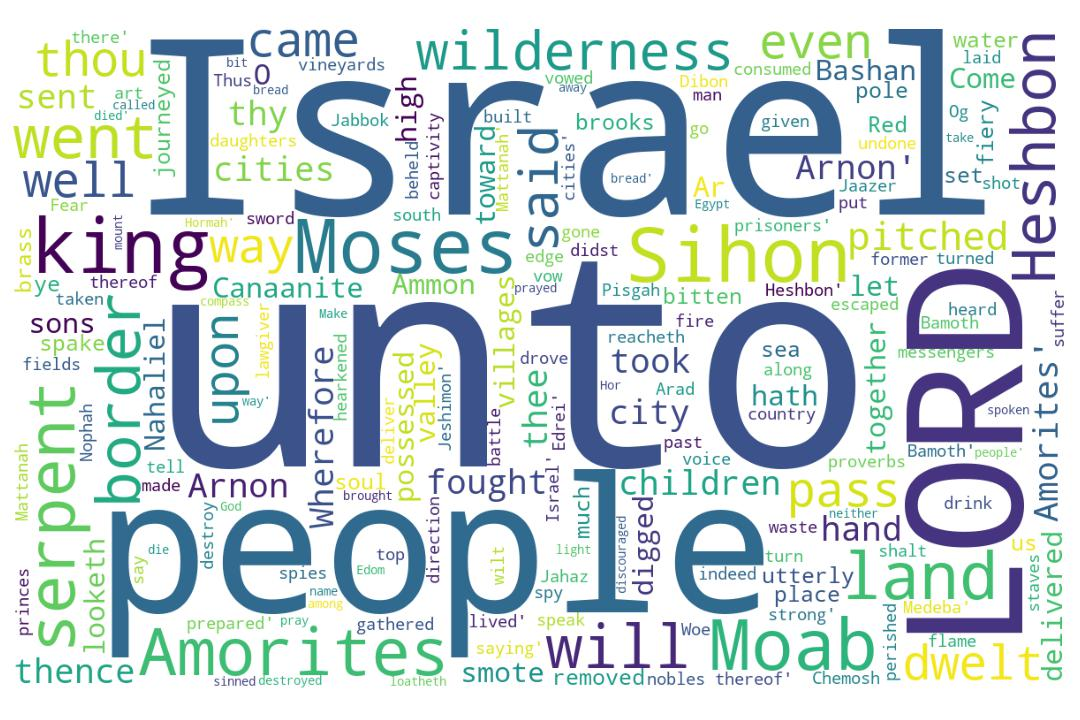
\includegraphics[width=\linewidth]{04OT-Numbers/Numbers21-WordCloud.jpg}
  \caption{Numbers 21 Word Cloud}
  \label{fig:Numbers 21 word Cloud}
\end{figure}


\marginpar{\scriptsize \centering \fcolorbox{bone}{lime}{\textbf{SIN, SERPENTS \& SWORDS}}\\ (Numbers 21)
\begin{compactenum}[I.][8]
     \item  The \textbf{Sin} of Discouragement \index[scripture]{Numbers!Num 21:04}   (Numbers 21:4)
    \item  \textbf{Serpents}  \index[scripture]{Numbers!Num 21:06}   (Numbers 21:6)
    \item  \textbf{Supplication}  \index[scripture]{Numbers!Num 21:07}   (Numbers 21:7)
    \item  The \textbf{Symbol}  \index[scripture]{Numbers!Num 21:09}   (Numbers 21:9)
    \item  A \textbf{Song}  \index[scripture]{Numbers!Num 21:17}   (Numbers 21:17)
    \item  The \textbf{Sword}  \index[scripture]{Numbers!Num 21:24}   (Numbers 21:24)
\end{compactenum}}




\footnote{\textcolor[rgb]{0.00,0.25,0.00}{\hyperlink{NumbersTOC}{Return to end of Table of Contents.}}}\footnote{\href{https://audiobible.com/bible/numbers_21.html}{\textcolor[cmyk]{0.99998,1,0,0}{Numbers 21 Audio}}}\textcolor[cmyk]{0.99998,1,0,0}{And \emph{when} king Arad the Canaanite, which dwelt in the south, heard tell that Israel came by the way of the spies; then he fought against Israel, and took \emph{some} of them prisoners.}
[2] \textcolor[cmyk]{0.99998,1,0,0}{And Israel vowed a vow unto the LORD, and said, If thou wilt indeed deliver this people into my hand, then I will utterly destroy their cities.}
[3] \textcolor[cmyk]{0.99998,1,0,0}{And the LORD hearkened to the voice of Israel, and delivered up the Canaanites; and they utterly destroyed them and their cities: and he called the name of the place Hormah.}\\
\\
\P \textcolor[cmyk]{0.99998,1,0,0}{And they journeyed from mount Hor by the way of the Red sea, to compass the land of Edom: and the soul of the people was much discouraged because of the way.}
[5] \textcolor[cmyk]{0.99998,1,0,0}{And the people spake against God, and against Moses, Wherefore have ye brought us up out of Egypt to die in the wilderness? for \emph{there} \emph{is} no bread, neither \emph{is} \emph{there} \emph{any} water; and our soul loatheth this light bread.}
[6] \textcolor[cmyk]{0.99998,1,0,0}{And the LORD sent fiery serpents among the people, and they bit the people; and much people of Israel died.}\\
\\
\P \textcolor[cmyk]{0.99998,1,0,0}{Therefore the people came to Moses, and said, We have sinned, for we have spoken against the LORD, and against thee; pray unto the LORD, that he take away the serpents from us. And Moses prayed for the people.}
[8] \textcolor[cmyk]{0.99998,1,0,0}{And the LORD said unto Moses, Make thee a fiery serpent, and set it upon a pole: and it shall come to pass, that every one that is bitten, when he looketh upon it, shall live.}
[9] \textcolor[cmyk]{0.99998,1,0,0}{And Moses made a serpent of brass, and put it upon a pole, and it came to pass, that if a serpent had bitten any man, when he beheld the serpent of brass, he lived.}\\
\\
\P \textcolor[cmyk]{0.99998,1,0,0}{And the children of Israel set forward, and pitched in Oboth.}
[11] \textcolor[cmyk]{0.99998,1,0,0}{And they journeyed from Oboth, and pitched at Ije-abarim, in the wilderness which \emph{is} before Moab, toward the sunrising.}
[12] \textcolor[cmyk]{0.99998,1,0,0}{From thence they removed, and pitched in the valley of Zared.}
[13] \textcolor[cmyk]{0.99998,1,0,0}{From thence they removed, and pitched on the other side of Arnon, which \emph{is} in the wilderness that cometh out of the coasts of the Amorites: for Arnon \emph{is} the border of Moab, between Moab and the Amorites.}
[14] \textcolor[cmyk]{0.99998,1,0,0}{Wherefore it is said in the book of the wars of the LORD, What he did in the Red sea, and in the brooks of Arnon,}
[15] \textcolor[cmyk]{0.99998,1,0,0}{And at the stream of the brooks that goeth down to the dwelling of Ar, and lieth upon the border of Moab.}
[16] \textcolor[cmyk]{0.99998,1,0,0}{And from thence \emph{they} \emph{went} to Beer: that \emph{is} the well whereof the LORD spake unto Moses, Gather the people together, and I will give them water.}
[17] \textcolor[cmyk]{0.99998,1,0,0}{Then Israel sang this song, Spring up, O well; sing ye unto it:}
[18] \textcolor[cmyk]{0.99998,1,0,0}{The princes digged the well, the nobles of the people digged it, by \emph{the} \emph{direction} \emph{of} the lawgiver, with their staves. And from the wilderness \emph{they} \emph{went} to Mattanah:}
[19] \textcolor[cmyk]{0.99998,1,0,0}{And from Mattanah to Nahaliel: and from Nahaliel to Bamoth:}
[20] \textcolor[cmyk]{0.99998,1,0,0}{And from Bamoth \emph{in} the valley, that \emph{is} in the country of Moab, to the top of Pisgah, which looketh toward Jeshimon.}\\
\\
\P \textcolor[cmyk]{0.99998,1,0,0}{And Israel sent messengers unto Sihon king of the Amorites, saying,}
[22] \textcolor[cmyk]{0.99998,1,0,0}{Let me pass through thy land: we will not turn into the fields, or into the vineyards; we will not drink \emph{of} the waters of the well: \emph{but} we will go along by the king's \emph{high} way, until we be past thy borders.}
[23] \textcolor[cmyk]{0.99998,1,0,0}{And Sihon would not suffer Israel to pass through \fcolorbox{bone}{bone}{his} border: but Sihon gathered all \fcolorbox{bone}{bone}{his} people together, and went out against Israel into the wilderness: and he came to Jahaz, and fought against Israel.}
[24] \textcolor[cmyk]{0.99998,1,0,0}{And Israel smote him with the edge of the sword, and possessed \fcolorbox{bone}{bone}{his} land from Arnon unto Jabbok, even unto the children of Ammon: for the border of the children of Ammon \emph{was} strong.}
[25] \textcolor[cmyk]{0.99998,1,0,0}{And Israel took all these cities: and Israel dwelt in all the cities of the Amorites, in Heshbon, and in all the villages thereof.}
[26] \textcolor[cmyk]{0.99998,1,0,0}{For Heshbon \emph{was} the city of Sihon the king of the Amorites, who had fought against the former king of Moab, and taken all \fcolorbox{bone}{bone}{his} land out of \fcolorbox{bone}{bone}{his} hand, even unto Arnon.}
[27] \textcolor[cmyk]{0.99998,1,0,0}{Wherefore they that speak in proverbs say, Come into Heshbon, let the city of Sihon be built and prepared:}
[28] \textcolor[cmyk]{0.99998,1,0,0}{For there is a fire gone out of Heshbon, a flame from the city of Sihon: it hath consumed Ar of Moab, \emph{and} the lords of the high places of Arnon.}
[29] \textcolor[cmyk]{0.99998,1,0,0}{Woe to thee, Moab! thou art undone, O people of Chemosh: he hath given \fcolorbox{bone}{bone}{his} sons that escaped, and \fcolorbox{bone}{bone}{his} daughters, into captivity unto Sihon king of the Amorites.}
[30] \textcolor[cmyk]{0.99998,1,0,0}{We have shot at them; Heshbon is perished even unto Dibon, and we have laid them waste even unto Nophah, which \emph{reacheth} unto Medeba.}\\
\\
\P \textcolor[cmyk]{0.99998,1,0,0}{Thus Israel dwelt in the land of the Amorites.}
[32] \textcolor[cmyk]{0.99998,1,0,0}{And Moses sent to spy out Jaazer, and they took the villages thereof, and drove out the Amorites that \emph{were} there.}
[33] \textcolor[cmyk]{0.99998,1,0,0}{And they turned and went up by the way of Bashan: and Og the king of Bashan went out against them, he, and all \fcolorbox{bone}{bone}{his} people, to the battle at Edrei.}
[34] \textcolor[cmyk]{0.99998,1,0,0}{And the LORD said unto Moses, Fear him not: for I have delivered him into thy hand, and all \fcolorbox{bone}{bone}{his} people, and \fcolorbox{bone}{bone}{his} land; and thou shalt do to him as thou didst unto Sihon king of the Amorites, which dwelt at Heshbon.}
[35] \textcolor[cmyk]{0.99998,1,0,0}{So they smote him, and \fcolorbox{bone}{bone}{his} sons, and all \fcolorbox{bone}{bone}{his} people, until there was none left him alive: and they possessed \fcolorbox{bone}{bone}{his} land.}
\index[NWIV]{33!Numbers!Num 21:1}\index[AWIP]{And!Numbers!Num 21:1}\index[AWIP]{\emph{when}!Numbers!Num 21:1}\index[AWIP]{king!Numbers!Num 21:1}\index[AWIP]{Arad!Numbers!Num 21:1}\index[AWIP]{the!Numbers!Num 21:1}\index[AWIP]{the!Numbers!Num 21:1 (2)}\index[AWIP]{the!Numbers!Num 21:1 (3)}\index[AWIP]{the!Numbers!Num 21:1 (4)}\index[AWIP]{Canaanite!Numbers!Num 21:1}\index[AWIP]{which!Numbers!Num 21:1}\index[AWIP]{dwelt!Numbers!Num 21:1}\index[AWIP]{in!Numbers!Num 21:1}\index[AWIP]{south!Numbers!Num 21:1}\index[AWIP]{heard!Numbers!Num 21:1}\index[AWIP]{tell!Numbers!Num 21:1}\index[AWIP]{that!Numbers!Num 21:1}\index[AWIP]{Israel!Numbers!Num 21:1}\index[AWIP]{Israel!Numbers!Num 21:1 (2)}\index[AWIP]{came!Numbers!Num 21:1}\index[AWIP]{by!Numbers!Num 21:1}\index[AWIP]{way!Numbers!Num 21:1}\index[AWIP]{of!Numbers!Num 21:1}\index[AWIP]{of!Numbers!Num 21:1 (2)}\index[AWIP]{spies!Numbers!Num 21:1}\index[AWIP]{then!Numbers!Num 21:1}\index[AWIP]{he!Numbers!Num 21:1}\index[AWIP]{fought!Numbers!Num 21:1}\index[AWIP]{against!Numbers!Num 21:1}\index[AWIP]{and!Numbers!Num 21:1}\index[AWIP]{took!Numbers!Num 21:1}\index[AWIP]{\emph{some}!Numbers!Num 21:1}\index[AWIP]{them!Numbers!Num 21:1}\index[AWIP]{prisoners!Numbers!Num 21:1}\index[AWIP]{\emph{when}!Numbers!Num 21:1}\index[AWIP]{\emph{some}!Numbers!Num 21:1}

\index[NWIV]{27!Numbers!Num 21:2}\index[AWIP]{And!Numbers!Num 21:2}\index[AWIP]{Israel!Numbers!Num 21:2}\index[AWIP]{vowed!Numbers!Num 21:2}\index[AWIP]{a!Numbers!Num 21:2}\index[AWIP]{vow!Numbers!Num 21:2}\index[AWIP]{unto!Numbers!Num 21:2}\index[AWIP]{the!Numbers!Num 21:2}\index[AWIP]{LORD!Numbers!Num 21:2}\index[AWIP]{and!Numbers!Num 21:2}\index[AWIP]{said!Numbers!Num 21:2}\index[AWIP]{If!Numbers!Num 21:2}\index[AWIP]{thou!Numbers!Num 21:2}\index[AWIP]{wilt!Numbers!Num 21:2}\index[AWIP]{indeed!Numbers!Num 21:2}\index[AWIP]{deliver!Numbers!Num 21:2}\index[AWIP]{this!Numbers!Num 21:2}\index[AWIP]{people!Numbers!Num 21:2}\index[AWIP]{into!Numbers!Num 21:2}\index[AWIP]{my!Numbers!Num 21:2}\index[AWIP]{hand!Numbers!Num 21:2}\index[AWIP]{then!Numbers!Num 21:2}\index[AWIP]{I!Numbers!Num 21:2}\index[AWIP]{will!Numbers!Num 21:2}\index[AWIP]{utterly!Numbers!Num 21:2}\index[AWIP]{destroy!Numbers!Num 21:2}\index[AWIP]{their!Numbers!Num 21:2}\index[AWIP]{cities!Numbers!Num 21:2}

\index[NWIV]{31!Numbers!Num 21:3}\index[AWIP]{And!Numbers!Num 21:3}\index[AWIP]{the!Numbers!Num 21:3}\index[AWIP]{the!Numbers!Num 21:3 (2)}\index[AWIP]{the!Numbers!Num 21:3 (3)}\index[AWIP]{the!Numbers!Num 21:3 (4)}\index[AWIP]{the!Numbers!Num 21:3 (5)}\index[AWIP]{LORD!Numbers!Num 21:3}\index[AWIP]{hearkened!Numbers!Num 21:3}\index[AWIP]{to!Numbers!Num 21:3}\index[AWIP]{voice!Numbers!Num 21:3}\index[AWIP]{of!Numbers!Num 21:3}\index[AWIP]{of!Numbers!Num 21:3 (2)}\index[AWIP]{Israel!Numbers!Num 21:3}\index[AWIP]{and!Numbers!Num 21:3}\index[AWIP]{and!Numbers!Num 21:3 (2)}\index[AWIP]{and!Numbers!Num 21:3 (3)}\index[AWIP]{and!Numbers!Num 21:3 (4)}\index[AWIP]{delivered!Numbers!Num 21:3}\index[AWIP]{up!Numbers!Num 21:3}\index[AWIP]{Canaanites!Numbers!Num 21:3}\index[AWIP]{they!Numbers!Num 21:3}\index[AWIP]{utterly!Numbers!Num 21:3}\index[AWIP]{destroyed!Numbers!Num 21:3}\index[AWIP]{them!Numbers!Num 21:3}\index[AWIP]{their!Numbers!Num 21:3}\index[AWIP]{cities!Numbers!Num 21:3}\index[AWIP]{he!Numbers!Num 21:3}\index[AWIP]{called!Numbers!Num 21:3}\index[AWIP]{name!Numbers!Num 21:3}\index[AWIP]{place!Numbers!Num 21:3}\index[AWIP]{Hormah!Numbers!Num 21:3}

\index[NWIV]{32!Numbers!Num 21:4}\index[AWIP]{And!Numbers!Num 21:4}\index[AWIP]{they!Numbers!Num 21:4}\index[AWIP]{journeyed!Numbers!Num 21:4}\index[AWIP]{from!Numbers!Num 21:4}\index[AWIP]{mount!Numbers!Num 21:4}\index[AWIP]{Hor!Numbers!Num 21:4}\index[AWIP]{by!Numbers!Num 21:4}\index[AWIP]{the!Numbers!Num 21:4}\index[AWIP]{the!Numbers!Num 21:4 (2)}\index[AWIP]{the!Numbers!Num 21:4 (3)}\index[AWIP]{the!Numbers!Num 21:4 (4)}\index[AWIP]{the!Numbers!Num 21:4 (5)}\index[AWIP]{the!Numbers!Num 21:4 (6)}\index[AWIP]{way!Numbers!Num 21:4}\index[AWIP]{way!Numbers!Num 21:4 (2)}\index[AWIP]{of!Numbers!Num 21:4}\index[AWIP]{of!Numbers!Num 21:4 (2)}\index[AWIP]{of!Numbers!Num 21:4 (3)}\index[AWIP]{of!Numbers!Num 21:4 (4)}\index[AWIP]{Red!Numbers!Num 21:4}\index[AWIP]{sea!Numbers!Num 21:4}\index[AWIP]{to!Numbers!Num 21:4}\index[AWIP]{compass!Numbers!Num 21:4}\index[AWIP]{land!Numbers!Num 21:4}\index[AWIP]{Edom!Numbers!Num 21:4}\index[AWIP]{and!Numbers!Num 21:4}\index[AWIP]{soul!Numbers!Num 21:4}\index[AWIP]{people!Numbers!Num 21:4}\index[AWIP]{was!Numbers!Num 21:4}\index[AWIP]{much!Numbers!Num 21:4}\index[AWIP]{discouraged!Numbers!Num 21:4}\index[AWIP]{because!Numbers!Num 21:4}

\index[NWIV]{40!Numbers!Num 21:5}\index[AWIP]{And!Numbers!Num 21:5}\index[AWIP]{the!Numbers!Num 21:5}\index[AWIP]{the!Numbers!Num 21:5 (2)}\index[AWIP]{people!Numbers!Num 21:5}\index[AWIP]{spake!Numbers!Num 21:5}\index[AWIP]{against!Numbers!Num 21:5}\index[AWIP]{against!Numbers!Num 21:5 (2)}\index[AWIP]{God!Numbers!Num 21:5}\index[AWIP]{and!Numbers!Num 21:5}\index[AWIP]{and!Numbers!Num 21:5 (2)}\index[AWIP]{Moses!Numbers!Num 21:5}\index[AWIP]{Wherefore!Numbers!Num 21:5}\index[AWIP]{have!Numbers!Num 21:5}\index[AWIP]{ye!Numbers!Num 21:5}\index[AWIP]{brought!Numbers!Num 21:5}\index[AWIP]{us!Numbers!Num 21:5}\index[AWIP]{up!Numbers!Num 21:5}\index[AWIP]{out!Numbers!Num 21:5}\index[AWIP]{of!Numbers!Num 21:5}\index[AWIP]{Egypt!Numbers!Num 21:5}\index[AWIP]{to!Numbers!Num 21:5}\index[AWIP]{die!Numbers!Num 21:5}\index[AWIP]{in!Numbers!Num 21:5}\index[AWIP]{wilderness?!Numbers!Num 21:5}\index[AWIP]{for!Numbers!Num 21:5}\index[AWIP]{\emph{there}!Numbers!Num 21:5}\index[AWIP]{\emph{there}!Numbers!Num 21:5 (2)}\index[AWIP]{\emph{is}!Numbers!Num 21:5}\index[AWIP]{\emph{is}!Numbers!Num 21:5 (2)}\index[AWIP]{no!Numbers!Num 21:5}\index[AWIP]{bread!Numbers!Num 21:5}\index[AWIP]{bread!Numbers!Num 21:5 (2)}\index[AWIP]{neither!Numbers!Num 21:5}\index[AWIP]{\emph{any}!Numbers!Num 21:5}\index[AWIP]{water!Numbers!Num 21:5}\index[AWIP]{our!Numbers!Num 21:5}\index[AWIP]{soul!Numbers!Num 21:5}\index[AWIP]{loatheth!Numbers!Num 21:5}\index[AWIP]{this!Numbers!Num 21:5}\index[AWIP]{light!Numbers!Num 21:5}\index[AWIP]{\emph{there}!Numbers!Num 21:5}\index[AWIP]{\emph{there}!Numbers!Num 21:5 (2)}\index[AWIP]{\emph{is}!Numbers!Num 21:5}\index[AWIP]{\emph{is}!Numbers!Num 21:5 (2)}\index[AWIP]{\emph{any}!Numbers!Num 21:5}

\index[NWIV]{20!Numbers!Num 21:6}\index[AWIP]{And!Numbers!Num 21:6}\index[AWIP]{the!Numbers!Num 21:6}\index[AWIP]{the!Numbers!Num 21:6 (2)}\index[AWIP]{the!Numbers!Num 21:6 (3)}\index[AWIP]{LORD!Numbers!Num 21:6}\index[AWIP]{sent!Numbers!Num 21:6}\index[AWIP]{fiery!Numbers!Num 21:6}\index[AWIP]{serpents!Numbers!Num 21:6}\index[AWIP]{among!Numbers!Num 21:6}\index[AWIP]{people!Numbers!Num 21:6}\index[AWIP]{people!Numbers!Num 21:6 (2)}\index[AWIP]{people!Numbers!Num 21:6 (3)}\index[AWIP]{and!Numbers!Num 21:6}\index[AWIP]{and!Numbers!Num 21:6 (2)}\index[AWIP]{they!Numbers!Num 21:6}\index[AWIP]{bit!Numbers!Num 21:6}\index[AWIP]{much!Numbers!Num 21:6}\index[AWIP]{of!Numbers!Num 21:6}\index[AWIP]{Israel!Numbers!Num 21:6}\index[AWIP]{died!Numbers!Num 21:6}

\index[NWIV]{39!Numbers!Num 21:7}\index[AWIP]{Therefore!Numbers!Num 21:7}\index[AWIP]{the!Numbers!Num 21:7}\index[AWIP]{the!Numbers!Num 21:7 (2)}\index[AWIP]{the!Numbers!Num 21:7 (3)}\index[AWIP]{the!Numbers!Num 21:7 (4)}\index[AWIP]{the!Numbers!Num 21:7 (5)}\index[AWIP]{people!Numbers!Num 21:7}\index[AWIP]{people!Numbers!Num 21:7 (2)}\index[AWIP]{came!Numbers!Num 21:7}\index[AWIP]{to!Numbers!Num 21:7}\index[AWIP]{Moses!Numbers!Num 21:7}\index[AWIP]{Moses!Numbers!Num 21:7 (2)}\index[AWIP]{and!Numbers!Num 21:7}\index[AWIP]{and!Numbers!Num 21:7 (2)}\index[AWIP]{said!Numbers!Num 21:7}\index[AWIP]{We!Numbers!Num 21:7}\index[AWIP]{have!Numbers!Num 21:7}\index[AWIP]{have!Numbers!Num 21:7 (2)}\index[AWIP]{sinned!Numbers!Num 21:7}\index[AWIP]{for!Numbers!Num 21:7}\index[AWIP]{for!Numbers!Num 21:7 (2)}\index[AWIP]{we!Numbers!Num 21:7}\index[AWIP]{spoken!Numbers!Num 21:7}\index[AWIP]{against!Numbers!Num 21:7}\index[AWIP]{against!Numbers!Num 21:7 (2)}\index[AWIP]{LORD!Numbers!Num 21:7}\index[AWIP]{LORD!Numbers!Num 21:7 (2)}\index[AWIP]{thee!Numbers!Num 21:7}\index[AWIP]{pray!Numbers!Num 21:7}\index[AWIP]{unto!Numbers!Num 21:7}\index[AWIP]{that!Numbers!Num 21:7}\index[AWIP]{he!Numbers!Num 21:7}\index[AWIP]{take!Numbers!Num 21:7}\index[AWIP]{away!Numbers!Num 21:7}\index[AWIP]{serpents!Numbers!Num 21:7}\index[AWIP]{from!Numbers!Num 21:7}\index[AWIP]{us!Numbers!Num 21:7}\index[AWIP]{And!Numbers!Num 21:7}\index[AWIP]{prayed!Numbers!Num 21:7}

\index[NWIV]{36!Numbers!Num 21:8}\index[AWIP]{And!Numbers!Num 21:8}\index[AWIP]{the!Numbers!Num 21:8}\index[AWIP]{LORD!Numbers!Num 21:8}\index[AWIP]{said!Numbers!Num 21:8}\index[AWIP]{unto!Numbers!Num 21:8}\index[AWIP]{Moses!Numbers!Num 21:8}\index[AWIP]{Make!Numbers!Num 21:8}\index[AWIP]{thee!Numbers!Num 21:8}\index[AWIP]{a!Numbers!Num 21:8}\index[AWIP]{a!Numbers!Num 21:8 (2)}\index[AWIP]{fiery!Numbers!Num 21:8}\index[AWIP]{serpent!Numbers!Num 21:8}\index[AWIP]{and!Numbers!Num 21:8}\index[AWIP]{and!Numbers!Num 21:8 (2)}\index[AWIP]{set!Numbers!Num 21:8}\index[AWIP]{it!Numbers!Num 21:8}\index[AWIP]{it!Numbers!Num 21:8 (2)}\index[AWIP]{it!Numbers!Num 21:8 (3)}\index[AWIP]{upon!Numbers!Num 21:8}\index[AWIP]{upon!Numbers!Num 21:8 (2)}\index[AWIP]{pole!Numbers!Num 21:8}\index[AWIP]{shall!Numbers!Num 21:8}\index[AWIP]{shall!Numbers!Num 21:8 (2)}\index[AWIP]{come!Numbers!Num 21:8}\index[AWIP]{to!Numbers!Num 21:8}\index[AWIP]{pass!Numbers!Num 21:8}\index[AWIP]{that!Numbers!Num 21:8}\index[AWIP]{that!Numbers!Num 21:8 (2)}\index[AWIP]{every!Numbers!Num 21:8}\index[AWIP]{one!Numbers!Num 21:8}\index[AWIP]{is!Numbers!Num 21:8}\index[AWIP]{bitten!Numbers!Num 21:8}\index[AWIP]{when!Numbers!Num 21:8}\index[AWIP]{he!Numbers!Num 21:8}\index[AWIP]{looketh!Numbers!Num 21:8}\index[AWIP]{live!Numbers!Num 21:8}

\index[NWIV]{35!Numbers!Num 21:9}\index[AWIP]{And!Numbers!Num 21:9}\index[AWIP]{Moses!Numbers!Num 21:9}\index[AWIP]{made!Numbers!Num 21:9}\index[AWIP]{a!Numbers!Num 21:9}\index[AWIP]{a!Numbers!Num 21:9 (2)}\index[AWIP]{a!Numbers!Num 21:9 (3)}\index[AWIP]{serpent!Numbers!Num 21:9}\index[AWIP]{serpent!Numbers!Num 21:9 (2)}\index[AWIP]{serpent!Numbers!Num 21:9 (3)}\index[AWIP]{of!Numbers!Num 21:9}\index[AWIP]{of!Numbers!Num 21:9 (2)}\index[AWIP]{brass!Numbers!Num 21:9}\index[AWIP]{brass!Numbers!Num 21:9 (2)}\index[AWIP]{and!Numbers!Num 21:9}\index[AWIP]{and!Numbers!Num 21:9 (2)}\index[AWIP]{put!Numbers!Num 21:9}\index[AWIP]{it!Numbers!Num 21:9}\index[AWIP]{it!Numbers!Num 21:9 (2)}\index[AWIP]{upon!Numbers!Num 21:9}\index[AWIP]{pole!Numbers!Num 21:9}\index[AWIP]{came!Numbers!Num 21:9}\index[AWIP]{to!Numbers!Num 21:9}\index[AWIP]{pass!Numbers!Num 21:9}\index[AWIP]{that!Numbers!Num 21:9}\index[AWIP]{if!Numbers!Num 21:9}\index[AWIP]{had!Numbers!Num 21:9}\index[AWIP]{bitten!Numbers!Num 21:9}\index[AWIP]{any!Numbers!Num 21:9}\index[AWIP]{man!Numbers!Num 21:9}\index[AWIP]{when!Numbers!Num 21:9}\index[AWIP]{he!Numbers!Num 21:9}\index[AWIP]{he!Numbers!Num 21:9 (2)}\index[AWIP]{beheld!Numbers!Num 21:9}\index[AWIP]{the!Numbers!Num 21:9}\index[AWIP]{lived!Numbers!Num 21:9}

\index[NWIV]{11!Numbers!Num 21:10}\index[AWIP]{And!Numbers!Num 21:10}\index[AWIP]{the!Numbers!Num 21:10}\index[AWIP]{children!Numbers!Num 21:10}\index[AWIP]{of!Numbers!Num 21:10}\index[AWIP]{Israel!Numbers!Num 21:10}\index[AWIP]{set!Numbers!Num 21:10}\index[AWIP]{forward!Numbers!Num 21:10}\index[AWIP]{and!Numbers!Num 21:10}\index[AWIP]{pitched!Numbers!Num 21:10}\index[AWIP]{in!Numbers!Num 21:10}\index[AWIP]{Oboth!Numbers!Num 21:10}

\index[NWIV]{19!Numbers!Num 21:11}\index[AWIP]{And!Numbers!Num 21:11}\index[AWIP]{they!Numbers!Num 21:11}\index[AWIP]{journeyed!Numbers!Num 21:11}\index[AWIP]{from!Numbers!Num 21:11}\index[AWIP]{Oboth!Numbers!Num 21:11}\index[AWIP]{and!Numbers!Num 21:11}\index[AWIP]{pitched!Numbers!Num 21:11}\index[AWIP]{at!Numbers!Num 21:11}\index[AWIP]{Ije-abarim!Numbers!Num 21:11}\index[AWIP]{in!Numbers!Num 21:11}\index[AWIP]{the!Numbers!Num 21:11}\index[AWIP]{the!Numbers!Num 21:11 (2)}\index[AWIP]{wilderness!Numbers!Num 21:11}\index[AWIP]{which!Numbers!Num 21:11}\index[AWIP]{\emph{is}!Numbers!Num 21:11}\index[AWIP]{before!Numbers!Num 21:11}\index[AWIP]{Moab!Numbers!Num 21:11}\index[AWIP]{toward!Numbers!Num 21:11}\index[AWIP]{sunrising!Numbers!Num 21:11}\index[AWIP]{\emph{is}!Numbers!Num 21:11}

\index[NWIV]{11!Numbers!Num 21:12}\index[AWIP]{From!Numbers!Num 21:12}\index[AWIP]{thence!Numbers!Num 21:12}\index[AWIP]{they!Numbers!Num 21:12}\index[AWIP]{removed!Numbers!Num 21:12}\index[AWIP]{and!Numbers!Num 21:12}\index[AWIP]{pitched!Numbers!Num 21:12}\index[AWIP]{in!Numbers!Num 21:12}\index[AWIP]{the!Numbers!Num 21:12}\index[AWIP]{valley!Numbers!Num 21:12}\index[AWIP]{of!Numbers!Num 21:12}\index[AWIP]{Zared!Numbers!Num 21:12}

\index[NWIV]{38!Numbers!Num 21:13}\index[AWIP]{From!Numbers!Num 21:13}\index[AWIP]{thence!Numbers!Num 21:13}\index[AWIP]{they!Numbers!Num 21:13}\index[AWIP]{removed!Numbers!Num 21:13}\index[AWIP]{and!Numbers!Num 21:13}\index[AWIP]{and!Numbers!Num 21:13 (2)}\index[AWIP]{pitched!Numbers!Num 21:13}\index[AWIP]{on!Numbers!Num 21:13}\index[AWIP]{the!Numbers!Num 21:13}\index[AWIP]{the!Numbers!Num 21:13 (2)}\index[AWIP]{the!Numbers!Num 21:13 (3)}\index[AWIP]{the!Numbers!Num 21:13 (4)}\index[AWIP]{the!Numbers!Num 21:13 (5)}\index[AWIP]{the!Numbers!Num 21:13 (6)}\index[AWIP]{other!Numbers!Num 21:13}\index[AWIP]{side!Numbers!Num 21:13}\index[AWIP]{of!Numbers!Num 21:13}\index[AWIP]{of!Numbers!Num 21:13 (2)}\index[AWIP]{of!Numbers!Num 21:13 (3)}\index[AWIP]{of!Numbers!Num 21:13 (4)}\index[AWIP]{Arnon!Numbers!Num 21:13}\index[AWIP]{Arnon!Numbers!Num 21:13 (2)}\index[AWIP]{which!Numbers!Num 21:13}\index[AWIP]{\emph{is}!Numbers!Num 21:13}\index[AWIP]{\emph{is}!Numbers!Num 21:13 (2)}\index[AWIP]{in!Numbers!Num 21:13}\index[AWIP]{wilderness!Numbers!Num 21:13}\index[AWIP]{that!Numbers!Num 21:13}\index[AWIP]{cometh!Numbers!Num 21:13}\index[AWIP]{out!Numbers!Num 21:13}\index[AWIP]{coasts!Numbers!Num 21:13}\index[AWIP]{Amorites!Numbers!Num 21:13}\index[AWIP]{Amorites!Numbers!Num 21:13 (2)}\index[AWIP]{for!Numbers!Num 21:13}\index[AWIP]{border!Numbers!Num 21:13}\index[AWIP]{Moab!Numbers!Num 21:13}\index[AWIP]{Moab!Numbers!Num 21:13 (2)}\index[AWIP]{between!Numbers!Num 21:13}\index[AWIP]{\emph{is}!Numbers!Num 21:13}\index[AWIP]{\emph{is}!Numbers!Num 21:13 (2)}

\index[NWIV]{26!Numbers!Num 21:14}\index[AWIP]{Wherefore!Numbers!Num 21:14}\index[AWIP]{it!Numbers!Num 21:14}\index[AWIP]{is!Numbers!Num 21:14}\index[AWIP]{said!Numbers!Num 21:14}\index[AWIP]{in!Numbers!Num 21:14}\index[AWIP]{in!Numbers!Num 21:14 (2)}\index[AWIP]{in!Numbers!Num 21:14 (3)}\index[AWIP]{the!Numbers!Num 21:14}\index[AWIP]{the!Numbers!Num 21:14 (2)}\index[AWIP]{the!Numbers!Num 21:14 (3)}\index[AWIP]{the!Numbers!Num 21:14 (4)}\index[AWIP]{the!Numbers!Num 21:14 (5)}\index[AWIP]{book!Numbers!Num 21:14}\index[AWIP]{of!Numbers!Num 21:14}\index[AWIP]{of!Numbers!Num 21:14 (2)}\index[AWIP]{of!Numbers!Num 21:14 (3)}\index[AWIP]{wars!Numbers!Num 21:14}\index[AWIP]{LORD!Numbers!Num 21:14}\index[AWIP]{What!Numbers!Num 21:14}\index[AWIP]{he!Numbers!Num 21:14}\index[AWIP]{did!Numbers!Num 21:14}\index[AWIP]{Red!Numbers!Num 21:14}\index[AWIP]{sea!Numbers!Num 21:14}\index[AWIP]{and!Numbers!Num 21:14}\index[AWIP]{brooks!Numbers!Num 21:14}\index[AWIP]{Arnon!Numbers!Num 21:14}

\index[NWIV]{22!Numbers!Num 21:15}\index[AWIP]{And!Numbers!Num 21:15}\index[AWIP]{at!Numbers!Num 21:15}\index[AWIP]{the!Numbers!Num 21:15}\index[AWIP]{the!Numbers!Num 21:15 (2)}\index[AWIP]{the!Numbers!Num 21:15 (3)}\index[AWIP]{the!Numbers!Num 21:15 (4)}\index[AWIP]{stream!Numbers!Num 21:15}\index[AWIP]{of!Numbers!Num 21:15}\index[AWIP]{of!Numbers!Num 21:15 (2)}\index[AWIP]{of!Numbers!Num 21:15 (3)}\index[AWIP]{brooks!Numbers!Num 21:15}\index[AWIP]{that!Numbers!Num 21:15}\index[AWIP]{goeth!Numbers!Num 21:15}\index[AWIP]{down!Numbers!Num 21:15}\index[AWIP]{to!Numbers!Num 21:15}\index[AWIP]{dwelling!Numbers!Num 21:15}\index[AWIP]{Ar!Numbers!Num 21:15}\index[AWIP]{and!Numbers!Num 21:15}\index[AWIP]{lieth!Numbers!Num 21:15}\index[AWIP]{upon!Numbers!Num 21:15}\index[AWIP]{border!Numbers!Num 21:15}\index[AWIP]{Moab!Numbers!Num 21:15}

\index[NWIV]{27!Numbers!Num 21:16}\index[AWIP]{And!Numbers!Num 21:16}\index[AWIP]{from!Numbers!Num 21:16}\index[AWIP]{thence!Numbers!Num 21:16}\index[AWIP]{\emph{they}!Numbers!Num 21:16}\index[AWIP]{\emph{went}!Numbers!Num 21:16}\index[AWIP]{to!Numbers!Num 21:16}\index[AWIP]{Beer!Numbers!Num 21:16}\index[AWIP]{that!Numbers!Num 21:16}\index[AWIP]{\emph{is}!Numbers!Num 21:16}\index[AWIP]{the!Numbers!Num 21:16}\index[AWIP]{the!Numbers!Num 21:16 (2)}\index[AWIP]{the!Numbers!Num 21:16 (3)}\index[AWIP]{well!Numbers!Num 21:16}\index[AWIP]{whereof!Numbers!Num 21:16}\index[AWIP]{LORD!Numbers!Num 21:16}\index[AWIP]{spake!Numbers!Num 21:16}\index[AWIP]{unto!Numbers!Num 21:16}\index[AWIP]{Moses!Numbers!Num 21:16}\index[AWIP]{Gather!Numbers!Num 21:16}\index[AWIP]{people!Numbers!Num 21:16}\index[AWIP]{together!Numbers!Num 21:16}\index[AWIP]{and!Numbers!Num 21:16}\index[AWIP]{I!Numbers!Num 21:16}\index[AWIP]{will!Numbers!Num 21:16}\index[AWIP]{give!Numbers!Num 21:16}\index[AWIP]{them!Numbers!Num 21:16}\index[AWIP]{water!Numbers!Num 21:16}\index[AWIP]{\emph{they}!Numbers!Num 21:16}\index[AWIP]{\emph{went}!Numbers!Num 21:16}\index[AWIP]{\emph{is}!Numbers!Num 21:16}

\index[NWIV]{13!Numbers!Num 21:17}\index[AWIP]{Then!Numbers!Num 21:17}\index[AWIP]{Israel!Numbers!Num 21:17}\index[AWIP]{sang!Numbers!Num 21:17}\index[AWIP]{this!Numbers!Num 21:17}\index[AWIP]{song!Numbers!Num 21:17}\index[AWIP]{Spring!Numbers!Num 21:17}\index[AWIP]{up!Numbers!Num 21:17}\index[AWIP]{O!Numbers!Num 21:17}\index[AWIP]{well!Numbers!Num 21:17}\index[AWIP]{sing!Numbers!Num 21:17}\index[AWIP]{ye!Numbers!Num 21:17}\index[AWIP]{unto!Numbers!Num 21:17}\index[AWIP]{it!Numbers!Num 21:17}

\index[NWIV]{29!Numbers!Num 21:18}\index[AWIP]{The!Numbers!Num 21:18}\index[AWIP]{princes!Numbers!Num 21:18}\index[AWIP]{digged!Numbers!Num 21:18}\index[AWIP]{digged!Numbers!Num 21:18 (2)}\index[AWIP]{the!Numbers!Num 21:18}\index[AWIP]{the!Numbers!Num 21:18 (2)}\index[AWIP]{the!Numbers!Num 21:18 (3)}\index[AWIP]{the!Numbers!Num 21:18 (4)}\index[AWIP]{the!Numbers!Num 21:18 (5)}\index[AWIP]{well!Numbers!Num 21:18}\index[AWIP]{nobles!Numbers!Num 21:18}\index[AWIP]{of!Numbers!Num 21:18}\index[AWIP]{people!Numbers!Num 21:18}\index[AWIP]{it!Numbers!Num 21:18}\index[AWIP]{by!Numbers!Num 21:18}\index[AWIP]{\emph{the}!Numbers!Num 21:18}\index[AWIP]{\emph{direction}!Numbers!Num 21:18}\index[AWIP]{\emph{of}!Numbers!Num 21:18}\index[AWIP]{lawgiver!Numbers!Num 21:18}\index[AWIP]{with!Numbers!Num 21:18}\index[AWIP]{their!Numbers!Num 21:18}\index[AWIP]{staves!Numbers!Num 21:18}\index[AWIP]{And!Numbers!Num 21:18}\index[AWIP]{from!Numbers!Num 21:18}\index[AWIP]{wilderness!Numbers!Num 21:18}\index[AWIP]{\emph{they}!Numbers!Num 21:18}\index[AWIP]{\emph{went}!Numbers!Num 21:18}\index[AWIP]{to!Numbers!Num 21:18}\index[AWIP]{Mattanah!Numbers!Num 21:18}\index[AWIP]{\emph{the}!Numbers!Num 21:18}\index[AWIP]{\emph{direction}!Numbers!Num 21:18}\index[AWIP]{\emph{of}!Numbers!Num 21:18}\index[AWIP]{\emph{they}!Numbers!Num 21:18}\index[AWIP]{\emph{went}!Numbers!Num 21:18}

\index[NWIV]{10!Numbers!Num 21:19}\index[AWIP]{And!Numbers!Num 21:19}\index[AWIP]{from!Numbers!Num 21:19}\index[AWIP]{from!Numbers!Num 21:19 (2)}\index[AWIP]{Mattanah!Numbers!Num 21:19}\index[AWIP]{to!Numbers!Num 21:19}\index[AWIP]{to!Numbers!Num 21:19 (2)}\index[AWIP]{Nahaliel!Numbers!Num 21:19}\index[AWIP]{Nahaliel!Numbers!Num 21:19 (2)}\index[AWIP]{and!Numbers!Num 21:19}\index[AWIP]{Bamoth!Numbers!Num 21:19}

\index[NWIV]{22!Numbers!Num 21:20}\index[AWIP]{And!Numbers!Num 21:20}\index[AWIP]{from!Numbers!Num 21:20}\index[AWIP]{Bamoth!Numbers!Num 21:20}\index[AWIP]{\emph{in}!Numbers!Num 21:20}\index[AWIP]{the!Numbers!Num 21:20}\index[AWIP]{the!Numbers!Num 21:20 (2)}\index[AWIP]{the!Numbers!Num 21:20 (3)}\index[AWIP]{valley!Numbers!Num 21:20}\index[AWIP]{that!Numbers!Num 21:20}\index[AWIP]{\emph{is}!Numbers!Num 21:20}\index[AWIP]{in!Numbers!Num 21:20}\index[AWIP]{country!Numbers!Num 21:20}\index[AWIP]{of!Numbers!Num 21:20}\index[AWIP]{of!Numbers!Num 21:20 (2)}\index[AWIP]{Moab!Numbers!Num 21:20}\index[AWIP]{to!Numbers!Num 21:20}\index[AWIP]{top!Numbers!Num 21:20}\index[AWIP]{Pisgah!Numbers!Num 21:20}\index[AWIP]{which!Numbers!Num 21:20}\index[AWIP]{looketh!Numbers!Num 21:20}\index[AWIP]{toward!Numbers!Num 21:20}\index[AWIP]{Jeshimon!Numbers!Num 21:20}\index[AWIP]{\emph{in}!Numbers!Num 21:20}\index[AWIP]{\emph{is}!Numbers!Num 21:20}

\index[NWIV]{11!Numbers!Num 21:21}\index[AWIP]{And!Numbers!Num 21:21}\index[AWIP]{Israel!Numbers!Num 21:21}\index[AWIP]{sent!Numbers!Num 21:21}\index[AWIP]{messengers!Numbers!Num 21:21}\index[AWIP]{unto!Numbers!Num 21:21}\index[AWIP]{Sihon!Numbers!Num 21:21}\index[AWIP]{king!Numbers!Num 21:21}\index[AWIP]{of!Numbers!Num 21:21}\index[AWIP]{the!Numbers!Num 21:21}\index[AWIP]{Amorites!Numbers!Num 21:21}\index[AWIP]{saying!Numbers!Num 21:21}

\index[NWIV]{43!Numbers!Num 21:22}\index[AWIP]{Let!Numbers!Num 21:22}\index[AWIP]{me!Numbers!Num 21:22}\index[AWIP]{pass!Numbers!Num 21:22}\index[AWIP]{through!Numbers!Num 21:22}\index[AWIP]{thy!Numbers!Num 21:22}\index[AWIP]{thy!Numbers!Num 21:22 (2)}\index[AWIP]{land!Numbers!Num 21:22}\index[AWIP]{we!Numbers!Num 21:22}\index[AWIP]{we!Numbers!Num 21:22 (2)}\index[AWIP]{we!Numbers!Num 21:22 (3)}\index[AWIP]{we!Numbers!Num 21:22 (4)}\index[AWIP]{will!Numbers!Num 21:22}\index[AWIP]{will!Numbers!Num 21:22 (2)}\index[AWIP]{will!Numbers!Num 21:22 (3)}\index[AWIP]{not!Numbers!Num 21:22}\index[AWIP]{not!Numbers!Num 21:22 (2)}\index[AWIP]{turn!Numbers!Num 21:22}\index[AWIP]{into!Numbers!Num 21:22}\index[AWIP]{into!Numbers!Num 21:22 (2)}\index[AWIP]{the!Numbers!Num 21:22}\index[AWIP]{the!Numbers!Num 21:22 (2)}\index[AWIP]{the!Numbers!Num 21:22 (3)}\index[AWIP]{the!Numbers!Num 21:22 (4)}\index[AWIP]{the!Numbers!Num 21:22 (5)}\index[AWIP]{fields!Numbers!Num 21:22}\index[AWIP]{or!Numbers!Num 21:22}\index[AWIP]{vineyards!Numbers!Num 21:22}\index[AWIP]{drink!Numbers!Num 21:22}\index[AWIP]{\emph{of}!Numbers!Num 21:22}\index[AWIP]{waters!Numbers!Num 21:22}\index[AWIP]{of!Numbers!Num 21:22}\index[AWIP]{well!Numbers!Num 21:22}\index[AWIP]{\emph{but}!Numbers!Num 21:22}\index[AWIP]{go!Numbers!Num 21:22}\index[AWIP]{along!Numbers!Num 21:22}\index[AWIP]{by!Numbers!Num 21:22}\index[AWIP]{king's!Numbers!Num 21:22}\index[AWIP]{\emph{high}!Numbers!Num 21:22}\index[AWIP]{way!Numbers!Num 21:22}\index[AWIP]{until!Numbers!Num 21:22}\index[AWIP]{be!Numbers!Num 21:22}\index[AWIP]{past!Numbers!Num 21:22}\index[AWIP]{borders!Numbers!Num 21:22}\index[AWIP]{\emph{of}!Numbers!Num 21:22}\index[AWIP]{\emph{but}!Numbers!Num 21:22}\index[AWIP]{\emph{high}!Numbers!Num 21:22}

\index[NWIV]{35!Numbers!Num 21:23}\index[AWIP]{And!Numbers!Num 21:23}\index[AWIP]{Sihon!Numbers!Num 21:23}\index[AWIP]{Sihon!Numbers!Num 21:23 (2)}\index[AWIP]{would!Numbers!Num 21:23}\index[AWIP]{not!Numbers!Num 21:23}\index[AWIP]{suffer!Numbers!Num 21:23}\index[AWIP]{Israel!Numbers!Num 21:23}\index[AWIP]{Israel!Numbers!Num 21:23 (2)}\index[AWIP]{Israel!Numbers!Num 21:23 (3)}\index[AWIP]{to!Numbers!Num 21:23}\index[AWIP]{to!Numbers!Num 21:23 (2)}\index[AWIP]{pass!Numbers!Num 21:23}\index[AWIP]{through!Numbers!Num 21:23}\index[AWIP]{his!Numbers!Num 21:23}\index[AWIP]{his!Numbers!Num 21:23 (2)}\index[AWIP]{border!Numbers!Num 21:23}\index[AWIP]{but!Numbers!Num 21:23}\index[AWIP]{gathered!Numbers!Num 21:23}\index[AWIP]{all!Numbers!Num 21:23}\index[AWIP]{people!Numbers!Num 21:23}\index[AWIP]{together!Numbers!Num 21:23}\index[AWIP]{and!Numbers!Num 21:23}\index[AWIP]{and!Numbers!Num 21:23 (2)}\index[AWIP]{and!Numbers!Num 21:23 (3)}\index[AWIP]{went!Numbers!Num 21:23}\index[AWIP]{out!Numbers!Num 21:23}\index[AWIP]{against!Numbers!Num 21:23}\index[AWIP]{against!Numbers!Num 21:23 (2)}\index[AWIP]{into!Numbers!Num 21:23}\index[AWIP]{the!Numbers!Num 21:23}\index[AWIP]{wilderness!Numbers!Num 21:23}\index[AWIP]{he!Numbers!Num 21:23}\index[AWIP]{came!Numbers!Num 21:23}\index[AWIP]{Jahaz!Numbers!Num 21:23}\index[AWIP]{fought!Numbers!Num 21:23}

\index[NWIV]{34!Numbers!Num 21:24}\index[AWIP]{And!Numbers!Num 21:24}\index[AWIP]{Israel!Numbers!Num 21:24}\index[AWIP]{smote!Numbers!Num 21:24}\index[AWIP]{him!Numbers!Num 21:24}\index[AWIP]{with!Numbers!Num 21:24}\index[AWIP]{the!Numbers!Num 21:24}\index[AWIP]{the!Numbers!Num 21:24 (2)}\index[AWIP]{the!Numbers!Num 21:24 (3)}\index[AWIP]{the!Numbers!Num 21:24 (4)}\index[AWIP]{the!Numbers!Num 21:24 (5)}\index[AWIP]{edge!Numbers!Num 21:24}\index[AWIP]{of!Numbers!Num 21:24}\index[AWIP]{of!Numbers!Num 21:24 (2)}\index[AWIP]{of!Numbers!Num 21:24 (3)}\index[AWIP]{of!Numbers!Num 21:24 (4)}\index[AWIP]{sword!Numbers!Num 21:24}\index[AWIP]{and!Numbers!Num 21:24}\index[AWIP]{possessed!Numbers!Num 21:24}\index[AWIP]{his!Numbers!Num 21:24}\index[AWIP]{land!Numbers!Num 21:24}\index[AWIP]{from!Numbers!Num 21:24}\index[AWIP]{Arnon!Numbers!Num 21:24}\index[AWIP]{unto!Numbers!Num 21:24}\index[AWIP]{unto!Numbers!Num 21:24 (2)}\index[AWIP]{Jabbok!Numbers!Num 21:24}\index[AWIP]{even!Numbers!Num 21:24}\index[AWIP]{children!Numbers!Num 21:24}\index[AWIP]{children!Numbers!Num 21:24 (2)}\index[AWIP]{Ammon!Numbers!Num 21:24}\index[AWIP]{Ammon!Numbers!Num 21:24 (2)}\index[AWIP]{for!Numbers!Num 21:24}\index[AWIP]{border!Numbers!Num 21:24}\index[AWIP]{\emph{was}!Numbers!Num 21:24}\index[AWIP]{strong!Numbers!Num 21:24}\index[AWIP]{\emph{was}!Numbers!Num 21:24}

\index[NWIV]{24!Numbers!Num 21:25}\index[AWIP]{And!Numbers!Num 21:25}\index[AWIP]{Israel!Numbers!Num 21:25}\index[AWIP]{Israel!Numbers!Num 21:25 (2)}\index[AWIP]{took!Numbers!Num 21:25}\index[AWIP]{all!Numbers!Num 21:25}\index[AWIP]{all!Numbers!Num 21:25 (2)}\index[AWIP]{all!Numbers!Num 21:25 (3)}\index[AWIP]{these!Numbers!Num 21:25}\index[AWIP]{cities!Numbers!Num 21:25}\index[AWIP]{cities!Numbers!Num 21:25 (2)}\index[AWIP]{and!Numbers!Num 21:25}\index[AWIP]{and!Numbers!Num 21:25 (2)}\index[AWIP]{dwelt!Numbers!Num 21:25}\index[AWIP]{in!Numbers!Num 21:25}\index[AWIP]{in!Numbers!Num 21:25 (2)}\index[AWIP]{in!Numbers!Num 21:25 (3)}\index[AWIP]{the!Numbers!Num 21:25}\index[AWIP]{the!Numbers!Num 21:25 (2)}\index[AWIP]{the!Numbers!Num 21:25 (3)}\index[AWIP]{of!Numbers!Num 21:25}\index[AWIP]{Amorites!Numbers!Num 21:25}\index[AWIP]{Heshbon!Numbers!Num 21:25}\index[AWIP]{villages!Numbers!Num 21:25}\index[AWIP]{thereof!Numbers!Num 21:25}

\index[NWIV]{33!Numbers!Num 21:26}\index[AWIP]{For!Numbers!Num 21:26}\index[AWIP]{Heshbon!Numbers!Num 21:26}\index[AWIP]{\emph{was}!Numbers!Num 21:26}\index[AWIP]{the!Numbers!Num 21:26}\index[AWIP]{the!Numbers!Num 21:26 (2)}\index[AWIP]{the!Numbers!Num 21:26 (3)}\index[AWIP]{the!Numbers!Num 21:26 (4)}\index[AWIP]{city!Numbers!Num 21:26}\index[AWIP]{of!Numbers!Num 21:26}\index[AWIP]{of!Numbers!Num 21:26 (2)}\index[AWIP]{of!Numbers!Num 21:26 (3)}\index[AWIP]{of!Numbers!Num 21:26 (4)}\index[AWIP]{Sihon!Numbers!Num 21:26}\index[AWIP]{king!Numbers!Num 21:26}\index[AWIP]{king!Numbers!Num 21:26 (2)}\index[AWIP]{Amorites!Numbers!Num 21:26}\index[AWIP]{who!Numbers!Num 21:26}\index[AWIP]{had!Numbers!Num 21:26}\index[AWIP]{fought!Numbers!Num 21:26}\index[AWIP]{against!Numbers!Num 21:26}\index[AWIP]{former!Numbers!Num 21:26}\index[AWIP]{Moab!Numbers!Num 21:26}\index[AWIP]{and!Numbers!Num 21:26}\index[AWIP]{taken!Numbers!Num 21:26}\index[AWIP]{all!Numbers!Num 21:26}\index[AWIP]{his!Numbers!Num 21:26}\index[AWIP]{his!Numbers!Num 21:26 (2)}\index[AWIP]{land!Numbers!Num 21:26}\index[AWIP]{out!Numbers!Num 21:26}\index[AWIP]{hand!Numbers!Num 21:26}\index[AWIP]{even!Numbers!Num 21:26}\index[AWIP]{unto!Numbers!Num 21:26}\index[AWIP]{Arnon!Numbers!Num 21:26}\index[AWIP]{\emph{was}!Numbers!Num 21:26}

\index[NWIV]{19!Numbers!Num 21:27}\index[AWIP]{Wherefore!Numbers!Num 21:27}\index[AWIP]{they!Numbers!Num 21:27}\index[AWIP]{that!Numbers!Num 21:27}\index[AWIP]{speak!Numbers!Num 21:27}\index[AWIP]{in!Numbers!Num 21:27}\index[AWIP]{proverbs!Numbers!Num 21:27}\index[AWIP]{say!Numbers!Num 21:27}\index[AWIP]{Come!Numbers!Num 21:27}\index[AWIP]{into!Numbers!Num 21:27}\index[AWIP]{Heshbon!Numbers!Num 21:27}\index[AWIP]{let!Numbers!Num 21:27}\index[AWIP]{the!Numbers!Num 21:27}\index[AWIP]{city!Numbers!Num 21:27}\index[AWIP]{of!Numbers!Num 21:27}\index[AWIP]{Sihon!Numbers!Num 21:27}\index[AWIP]{be!Numbers!Num 21:27}\index[AWIP]{built!Numbers!Num 21:27}\index[AWIP]{and!Numbers!Num 21:27}\index[AWIP]{prepared!Numbers!Num 21:27}

\index[NWIV]{31!Numbers!Num 21:28}\index[AWIP]{For!Numbers!Num 21:28}\index[AWIP]{there!Numbers!Num 21:28}\index[AWIP]{is!Numbers!Num 21:28}\index[AWIP]{a!Numbers!Num 21:28}\index[AWIP]{a!Numbers!Num 21:28 (2)}\index[AWIP]{fire!Numbers!Num 21:28}\index[AWIP]{gone!Numbers!Num 21:28}\index[AWIP]{out!Numbers!Num 21:28}\index[AWIP]{of!Numbers!Num 21:28}\index[AWIP]{of!Numbers!Num 21:28 (2)}\index[AWIP]{of!Numbers!Num 21:28 (3)}\index[AWIP]{of!Numbers!Num 21:28 (4)}\index[AWIP]{of!Numbers!Num 21:28 (5)}\index[AWIP]{Heshbon!Numbers!Num 21:28}\index[AWIP]{flame!Numbers!Num 21:28}\index[AWIP]{from!Numbers!Num 21:28}\index[AWIP]{the!Numbers!Num 21:28}\index[AWIP]{the!Numbers!Num 21:28 (2)}\index[AWIP]{the!Numbers!Num 21:28 (3)}\index[AWIP]{city!Numbers!Num 21:28}\index[AWIP]{Sihon!Numbers!Num 21:28}\index[AWIP]{it!Numbers!Num 21:28}\index[AWIP]{hath!Numbers!Num 21:28}\index[AWIP]{consumed!Numbers!Num 21:28}\index[AWIP]{Ar!Numbers!Num 21:28}\index[AWIP]{Moab!Numbers!Num 21:28}\index[AWIP]{\emph{and}!Numbers!Num 21:28}\index[AWIP]{lords!Numbers!Num 21:28}\index[AWIP]{high!Numbers!Num 21:28}\index[AWIP]{places!Numbers!Num 21:28}\index[AWIP]{Arnon!Numbers!Num 21:28}\index[AWIP]{\emph{and}!Numbers!Num 21:28}

\index[NWIV]{29!Numbers!Num 21:29}\index[AWIP]{Woe!Numbers!Num 21:29}\index[AWIP]{to!Numbers!Num 21:29}\index[AWIP]{thee!Numbers!Num 21:29}\index[AWIP]{Moab!!Numbers!Num 21:29}\index[AWIP]{thou!Numbers!Num 21:29}\index[AWIP]{art!Numbers!Num 21:29}\index[AWIP]{undone!Numbers!Num 21:29}\index[AWIP]{O!Numbers!Num 21:29}\index[AWIP]{people!Numbers!Num 21:29}\index[AWIP]{of!Numbers!Num 21:29}\index[AWIP]{of!Numbers!Num 21:29 (2)}\index[AWIP]{Chemosh!Numbers!Num 21:29}\index[AWIP]{he!Numbers!Num 21:29}\index[AWIP]{hath!Numbers!Num 21:29}\index[AWIP]{given!Numbers!Num 21:29}\index[AWIP]{his!Numbers!Num 21:29}\index[AWIP]{his!Numbers!Num 21:29 (2)}\index[AWIP]{sons!Numbers!Num 21:29}\index[AWIP]{that!Numbers!Num 21:29}\index[AWIP]{escaped!Numbers!Num 21:29}\index[AWIP]{and!Numbers!Num 21:29}\index[AWIP]{daughters!Numbers!Num 21:29}\index[AWIP]{into!Numbers!Num 21:29}\index[AWIP]{captivity!Numbers!Num 21:29}\index[AWIP]{unto!Numbers!Num 21:29}\index[AWIP]{Sihon!Numbers!Num 21:29}\index[AWIP]{king!Numbers!Num 21:29}\index[AWIP]{the!Numbers!Num 21:29}\index[AWIP]{Amorites!Numbers!Num 21:29}

\index[NWIV]{24!Numbers!Num 21:30}\index[AWIP]{We!Numbers!Num 21:30}\index[AWIP]{have!Numbers!Num 21:30}\index[AWIP]{have!Numbers!Num 21:30 (2)}\index[AWIP]{shot!Numbers!Num 21:30}\index[AWIP]{at!Numbers!Num 21:30}\index[AWIP]{them!Numbers!Num 21:30}\index[AWIP]{them!Numbers!Num 21:30 (2)}\index[AWIP]{Heshbon!Numbers!Num 21:30}\index[AWIP]{is!Numbers!Num 21:30}\index[AWIP]{perished!Numbers!Num 21:30}\index[AWIP]{even!Numbers!Num 21:30}\index[AWIP]{even!Numbers!Num 21:30 (2)}\index[AWIP]{unto!Numbers!Num 21:30}\index[AWIP]{unto!Numbers!Num 21:30 (2)}\index[AWIP]{unto!Numbers!Num 21:30 (3)}\index[AWIP]{Dibon!Numbers!Num 21:30}\index[AWIP]{and!Numbers!Num 21:30}\index[AWIP]{we!Numbers!Num 21:30}\index[AWIP]{laid!Numbers!Num 21:30}\index[AWIP]{waste!Numbers!Num 21:30}\index[AWIP]{Nophah!Numbers!Num 21:30}\index[AWIP]{which!Numbers!Num 21:30}\index[AWIP]{\emph{reacheth}!Numbers!Num 21:30}\index[AWIP]{Medeba!Numbers!Num 21:30}\index[AWIP]{\emph{reacheth}!Numbers!Num 21:30}

\index[NWIV]{9!Numbers!Num 21:31}\index[AWIP]{Thus!Numbers!Num 21:31}\index[AWIP]{Israel!Numbers!Num 21:31}\index[AWIP]{dwelt!Numbers!Num 21:31}\index[AWIP]{in!Numbers!Num 21:31}\index[AWIP]{the!Numbers!Num 21:31}\index[AWIP]{the!Numbers!Num 21:31 (2)}\index[AWIP]{land!Numbers!Num 21:31}\index[AWIP]{of!Numbers!Num 21:31}\index[AWIP]{Amorites!Numbers!Num 21:31}

\index[NWIV]{21!Numbers!Num 21:32}\index[AWIP]{And!Numbers!Num 21:32}\index[AWIP]{Moses!Numbers!Num 21:32}\index[AWIP]{sent!Numbers!Num 21:32}\index[AWIP]{to!Numbers!Num 21:32}\index[AWIP]{spy!Numbers!Num 21:32}\index[AWIP]{out!Numbers!Num 21:32}\index[AWIP]{out!Numbers!Num 21:32 (2)}\index[AWIP]{Jaazer!Numbers!Num 21:32}\index[AWIP]{and!Numbers!Num 21:32}\index[AWIP]{and!Numbers!Num 21:32 (2)}\index[AWIP]{they!Numbers!Num 21:32}\index[AWIP]{took!Numbers!Num 21:32}\index[AWIP]{the!Numbers!Num 21:32}\index[AWIP]{the!Numbers!Num 21:32 (2)}\index[AWIP]{villages!Numbers!Num 21:32}\index[AWIP]{thereof!Numbers!Num 21:32}\index[AWIP]{drove!Numbers!Num 21:32}\index[AWIP]{Amorites!Numbers!Num 21:32}\index[AWIP]{that!Numbers!Num 21:32}\index[AWIP]{\emph{were}!Numbers!Num 21:32}\index[AWIP]{there!Numbers!Num 21:32}\index[AWIP]{\emph{were}!Numbers!Num 21:32}

\index[NWIV]{31!Numbers!Num 21:33}\index[AWIP]{And!Numbers!Num 21:33}\index[AWIP]{they!Numbers!Num 21:33}\index[AWIP]{turned!Numbers!Num 21:33}\index[AWIP]{and!Numbers!Num 21:33}\index[AWIP]{and!Numbers!Num 21:33 (2)}\index[AWIP]{and!Numbers!Num 21:33 (3)}\index[AWIP]{went!Numbers!Num 21:33}\index[AWIP]{went!Numbers!Num 21:33 (2)}\index[AWIP]{up!Numbers!Num 21:33}\index[AWIP]{by!Numbers!Num 21:33}\index[AWIP]{the!Numbers!Num 21:33}\index[AWIP]{the!Numbers!Num 21:33 (2)}\index[AWIP]{the!Numbers!Num 21:33 (3)}\index[AWIP]{way!Numbers!Num 21:33}\index[AWIP]{of!Numbers!Num 21:33}\index[AWIP]{of!Numbers!Num 21:33 (2)}\index[AWIP]{Bashan!Numbers!Num 21:33}\index[AWIP]{Bashan!Numbers!Num 21:33 (2)}\index[AWIP]{Og!Numbers!Num 21:33}\index[AWIP]{king!Numbers!Num 21:33}\index[AWIP]{out!Numbers!Num 21:33}\index[AWIP]{against!Numbers!Num 21:33}\index[AWIP]{them!Numbers!Num 21:33}\index[AWIP]{he!Numbers!Num 21:33}\index[AWIP]{all!Numbers!Num 21:33}\index[AWIP]{his!Numbers!Num 21:33}\index[AWIP]{people!Numbers!Num 21:33}\index[AWIP]{to!Numbers!Num 21:33}\index[AWIP]{battle!Numbers!Num 21:33}\index[AWIP]{at!Numbers!Num 21:33}\index[AWIP]{Edrei!Numbers!Num 21:33}

\index[NWIV]{43!Numbers!Num 21:34}\index[AWIP]{And!Numbers!Num 21:34}\index[AWIP]{the!Numbers!Num 21:34}\index[AWIP]{the!Numbers!Num 21:34 (2)}\index[AWIP]{LORD!Numbers!Num 21:34}\index[AWIP]{said!Numbers!Num 21:34}\index[AWIP]{unto!Numbers!Num 21:34}\index[AWIP]{unto!Numbers!Num 21:34 (2)}\index[AWIP]{Moses!Numbers!Num 21:34}\index[AWIP]{Fear!Numbers!Num 21:34}\index[AWIP]{him!Numbers!Num 21:34}\index[AWIP]{him!Numbers!Num 21:34 (2)}\index[AWIP]{him!Numbers!Num 21:34 (3)}\index[AWIP]{not!Numbers!Num 21:34}\index[AWIP]{for!Numbers!Num 21:34}\index[AWIP]{I!Numbers!Num 21:34}\index[AWIP]{have!Numbers!Num 21:34}\index[AWIP]{delivered!Numbers!Num 21:34}\index[AWIP]{into!Numbers!Num 21:34}\index[AWIP]{thy!Numbers!Num 21:34}\index[AWIP]{hand!Numbers!Num 21:34}\index[AWIP]{and!Numbers!Num 21:34}\index[AWIP]{and!Numbers!Num 21:34 (2)}\index[AWIP]{and!Numbers!Num 21:34 (3)}\index[AWIP]{all!Numbers!Num 21:34}\index[AWIP]{his!Numbers!Num 21:34}\index[AWIP]{his!Numbers!Num 21:34 (2)}\index[AWIP]{people!Numbers!Num 21:34}\index[AWIP]{land!Numbers!Num 21:34}\index[AWIP]{thou!Numbers!Num 21:34}\index[AWIP]{thou!Numbers!Num 21:34 (2)}\index[AWIP]{shalt!Numbers!Num 21:34}\index[AWIP]{do!Numbers!Num 21:34}\index[AWIP]{to!Numbers!Num 21:34}\index[AWIP]{as!Numbers!Num 21:34}\index[AWIP]{didst!Numbers!Num 21:34}\index[AWIP]{Sihon!Numbers!Num 21:34}\index[AWIP]{king!Numbers!Num 21:34}\index[AWIP]{of!Numbers!Num 21:34}\index[AWIP]{Amorites!Numbers!Num 21:34}\index[AWIP]{which!Numbers!Num 21:34}\index[AWIP]{dwelt!Numbers!Num 21:34}\index[AWIP]{at!Numbers!Num 21:34}\index[AWIP]{Heshbon!Numbers!Num 21:34}

\index[NWIV]{23!Numbers!Num 21:35}\index[AWIP]{So!Numbers!Num 21:35}\index[AWIP]{they!Numbers!Num 21:35}\index[AWIP]{they!Numbers!Num 21:35 (2)}\index[AWIP]{smote!Numbers!Num 21:35}\index[AWIP]{him!Numbers!Num 21:35}\index[AWIP]{him!Numbers!Num 21:35 (2)}\index[AWIP]{and!Numbers!Num 21:35}\index[AWIP]{and!Numbers!Num 21:35 (2)}\index[AWIP]{and!Numbers!Num 21:35 (3)}\index[AWIP]{his!Numbers!Num 21:35}\index[AWIP]{his!Numbers!Num 21:35 (2)}\index[AWIP]{his!Numbers!Num 21:35 (3)}\index[AWIP]{sons!Numbers!Num 21:35}\index[AWIP]{all!Numbers!Num 21:35}\index[AWIP]{people!Numbers!Num 21:35}\index[AWIP]{until!Numbers!Num 21:35}\index[AWIP]{there!Numbers!Num 21:35}\index[AWIP]{was!Numbers!Num 21:35}\index[AWIP]{none!Numbers!Num 21:35}\index[AWIP]{left!Numbers!Num 21:35}\index[AWIP]{alive!Numbers!Num 21:35}\index[AWIP]{possessed!Numbers!Num 21:35}\index[AWIP]{land!Numbers!Num 21:35}


\section{Number 21 Outlines}

\subsection{My Outlines}

\subsubsection{Sin, Serpents \& Swords}
%Practical Wisdom from Proverbs 6:\footnote{03 November 2014, Keith Anthony}
\index[speaker]{Keith Anthony!Numbers 21 (Sin, Serpents \& Swords}
\index[series]{Numbers (Keith Anthony)!Numbers 21 (Sin, Serpents \& Swords)}
\index[date]{2018/02/17!Numbers 21 (Sin, Serpents \& Swords (Keith Anthony)}

\begin{compactenum}[I.]
    \item  The \textbf{Sin} of Discouragement \index[scripture]{Numbers!Num 21:04}   (Numbers 21:4)
    \item  \textbf{Serpents}  \index[scripture]{Numbers!Num 21:06}   (Numbers 21:6)
    \item  \textbf{Supplication}  \index[scripture]{Numbers!Num 21:07}   (Numbers 21:7)
    \item  The \textbf{Symbol}  \index[scripture]{Numbers!Num 21:09}   (Numbers 21:9)
    \item  A \textbf{Song}  \index[scripture]{Numbers!Num 21:17}   (Numbers 21:17)
    \item  The \textbf{Sword}  \index[scripture]{Numbers!Num 21:24}   (Numbers 21:24)
\end{compactenum}




\subsection{Outlines from Others}
\section{Numbers 21 Comments}

\subsection{Numeric Nuggets}
\textbf{13: } Verse 17 has 13 words, 13 unique words.. The word ``his'' is found 13 time sin the chapter.
\subsection{Numbers 21 Repeated Phrases}


%%%%%%%%%%
%%%%%%%%%%
\normalsize
 
\begin{center}
\begin{longtable}{|c|c|}
\caption[Numbers 21 Repeated Phrases]{Numbers 21 Repeated Phrases}\label{table:Repeated Phrases Numbers 21} \\
\hline \multicolumn{1}{|c|}{\textbf{Phrase}} & \multicolumn{1}{c|}{\textbf{Frequency}} \\ \hline 
\endfirsthead
 
\multicolumn{2}{c}
{{\bfseries \tablename\ \thetable{} -- continued from previous page}} \\  
\hline \multicolumn{1}{|c|}{\textbf{Phrase}} & \multicolumn{1}{c|}{\textbf{Frequency}} \\ \hline 
\endhead
 
\hline \multicolumn{2}{c}{{ }} \\ \hline
\endfoot 
of the & 21\\ \hline 
in the & 10\\ \hline 
the LORD & 9\\ \hline 
the Amorites & 9\\ \hline 
the people & 8\\ \hline 
of the Amorites & 7\\ \hline 
And the & 6\\ \hline 
king of & 6\\ \hline 
the wilderness & 5\\ \hline 
of Moab & 5\\ \hline 
all his & 5\\ \hline 
by the & 4\\ \hline 
the way & 4\\ \hline 
And Israel & 4\\ \hline 
And the LORD & 4\\ \hline 
to the & 4\\ \hline 
and they & 4\\ \hline 
out of & 4\\ \hline 
and pitched & 4\\ \hline 
And from & 4\\ \hline 
king of the & 4\\ \hline 
king of the Amorites & 4\\ \hline 
all his people & 4\\ \hline 
his people & 4\\ \hline 
his land & 4\\ \hline 
even unto & 4\\ \hline 
dwelt in & 3\\ \hline 
by the way & 3\\ \hline 
by the way of & 3\\ \hline 
the way of & 3\\ \hline 
way of & 3\\ \hline 
fought against & 3\\ \hline 
against Israel & 3\\ \hline 
unto the & 3\\ \hline 
of Israel & 3\\ \hline 
And they & 3\\ \hline 
in the wilderness & 3\\ \hline 
people and & 3\\ \hline 
came to & 3\\ \hline 
And Moses & 3\\ \hline 
unto Moses & 3\\ \hline 
to pass & 3\\ \hline 
the children & 3\\ \hline 
the children of & 3\\ \hline 
children of & 3\\ \hline 
of Arnon & 3\\ \hline 
the border & 3\\ \hline 
the border of & 3\\ \hline 
border of & 3\\ \hline 
the well & 3\\ \hline 
unto Sihon & 3\\ \hline 
unto Sihon king & 3\\ \hline 
unto Sihon king of & 3\\ \hline 
unto Sihon king of the & 3\\ \hline 
unto Sihon king of the Amorites & 3\\ \hline 
Sihon king & 3\\ \hline 
Sihon king of & 3\\ \hline 
Sihon king of the & 3\\ \hline 
Sihon king of the Amorites & 3\\ \hline 
we will & 3\\ \hline 
into the & 3\\ \hline 
the city & 3\\ \hline 
the city of & 3\\ \hline 
the city of Sihon & 3\\ \hline 
city of & 3\\ \hline 
city of Sihon & 3\\ \hline 
of Sihon & 3\\ \hline 
and his & 3\\ \hline 
and all & 3\\ \hline 
and all his & 3\\ \hline 
and all his people & 3\\ \hline 
\end{longtable}
\end{center}



%%%%%%%%%%
%%%%%%%%%%



\section{Numbers 21 Statistics}


%%%%%%%%%%%%%%%%%%%%%%%%%%%
%%%%% Word Statistics
%%%%%%%%%%%%%%%%%%%%%%%%%%


\normalsize



\subsection{Chapter Word Statistics}


%%%%%%%%%%
%%%%%%%%%%
 
\begin{center}
\begin{longtable}{l|c|c|c|c}
\caption[Stats for Numbers 21]{Stats for Numbers 21} \label{table:Stats for Numbers 21} \\ 
\hline \multicolumn{1}{|c|}{\textbf{Verse(s)}} & \multicolumn{1}{|c|}{\textbf{Count}} & \multicolumn{1}{|c|}{\textbf{Unique}} & \multicolumn{1}{|c|}{\textbf{Italics}} & \multicolumn{1}{|c|}{\textbf{Uniq Italic}}  \\ \hline 
\endfirsthead
 
\multicolumn{5}{c}
{{\bfseries \tablename\ \thetable{} -- continued from previous page}} \\  
\hline \multicolumn{1}{|c|}{\textbf{Verse(s)}} & \multicolumn{1}{|c|}{\textbf{Count}} & \multicolumn{1}{|c|}{\textbf{Unique}} & \multicolumn{1}{|c|}{\textbf{Italics}} & \multicolumn{1}{|c|}{\textbf{Uniq Italic}}  \\ \hline 
\endhead
 
\hline \multicolumn{5}{|r|}{{Continued if needed}} \\ \hline
\endfoot 
1 & 33 & 28 & 2 & 2\\ \hline
2 & 27 & 27 & 0 & 0\\ \hline
3 & 31 & 23 & 0 & 0\\ \hline
4 & 32 & 23 & 0 & 0\\ \hline
5 & 40 & 34 & 5 & 3\\ \hline
6 & 20 & 15 & 0 & 0\\ \hline
7 & 39 & 28 & 0 & 0\\ \hline
8 & 36 & 29 & 0 & 0\\ \hline
9 & 35 & 26 & 0 & 0\\ \hline
10 & 11 & 11 & 0 & 0\\ \hline
11 & 19 & 18 & 1 & 1\\ \hline
12 & 11 & 11 & 0 & 0\\ \hline
13 & 38 & 25 & 2 & 1\\ \hline
14 & 26 & 18 & 0 & 0\\ \hline
15 & 22 & 17 & 0 & 0\\ \hline
16 & 27 & 25 & 3 & 3\\ \hline
17 & 13 & 13 & 0 & 0\\ \hline
18 & 29 & 24 & 5 & 5\\ \hline
19 & 10 & 7 & 0 & 0\\ \hline
20 & 22 & 19 & 2 & 2\\ \hline
21 & 11 & 11 & 0 & 0\\ \hline
22 & 43 & 31 & 3 & 3\\ \hline
23 & 35 & 27 & 0 & 0\\ \hline
24 & 34 & 24 & 1 & 1\\ \hline
25 & 24 & 15 & 0 & 0\\ \hline
26 & 33 & 25 & 1 & 1\\ \hline
27 & 19 & 19 & 0 & 0\\ \hline
28 & 31 & 24 & 1 & 1\\ \hline
29 & 29 & 27 & 0 & 0\\ \hline
30 & 24 & 19 & 1 & 1\\ \hline
31 & 9 & 8 & 0 & 0\\ \hline
32 & 21 & 18 & 1 & 1\\ \hline
33 & 31 & 24 & 0 & 0\\ \hline
34 & 43 & 35 & 0 & 0\\ \hline
35 & 23 & 17 & 0 & 0\\ \hline
\hline \hline
Total & 931 & 310 & 28 & 17



\end{longtable}
\end{center}

%%%%%%%%%%
%%%%%%%%%%
 
\subsection{Words by Frequency}

\begin{center}
\begin{longtable}{l|r}
\caption[Word Frequencies in Numbers 21]{Word Frequencies in Numbers 21} \label{table:WordsIn-Numbers-21} \\ 
\hline \multicolumn{1}{|c|}{\textbf{Word}} & \multicolumn{1}{c|}{\textbf{Frequency}} \\ \hline 
\endfirsthead
 
\multicolumn{2}{c}
{{\bfseries \tablename\ \thetable{} -- continued from previous page}} \\ 
\hline \multicolumn{1}{|c|}{\textbf{Word}} & \multicolumn{1}{c|}{\textbf{Frequency}} \\ \hline 
\endhead
 
\hline \multicolumn{2}{|r|}{{Continued if needed}} \\ \hline
\endfoot
 
\hline \hline
\endlastfoot
the & 91 \\ \hline
of & 50 \\ \hline
and & 47 \\ \hline
And & 23 \\ \hline
to & 18 \\ \hline
in & 15 \\ \hline
Israel & 15 \\ \hline
unto & 15 \\ \hline
people & 15 \\ \hline
his & 13 \\ \hline
that & 12 \\ \hline
they & 11 \\ \hline
he & 10 \\ \hline
from & 10 \\ \hline
against & 9 \\ \hline
LORD & 9 \\ \hline
it & 9 \\ \hline
Amorites & 9 \\ \hline
a & 8 \\ \hline
Moses & 8 \\ \hline
out & 8 \\ \hline
Moab & 8 \\ \hline
Sihon & 8 \\ \hline
all & 8 \\ \hline
king & 7 \\ \hline
into & 7 \\ \hline
land & 7 \\ \hline
\emph{is} & 7 \\ \hline
which & 6 \\ \hline
them & 6 \\ \hline
have & 6 \\ \hline
for & 6 \\ \hline
we & 6 \\ \hline
Arnon & 6 \\ \hline
him & 6 \\ \hline
Heshbon & 6 \\ \hline
by & 5 \\ \hline
way & 5 \\ \hline
said & 5 \\ \hline
will & 5 \\ \hline
wilderness & 5 \\ \hline
at & 5 \\ \hline
dwelt & 4 \\ \hline
came & 4 \\ \hline
thou & 4 \\ \hline
cities & 4 \\ \hline
up & 4 \\ \hline
serpent & 4 \\ \hline
upon & 4 \\ \hline
pass & 4 \\ \hline
is & 4 \\ \hline
pitched & 4 \\ \hline
border & 4 \\ \hline
well & 4 \\ \hline
not & 4 \\ \hline
even & 4 \\ \hline
fought & 3 \\ \hline
took & 3 \\ \hline
this & 3 \\ \hline
hand & 3 \\ \hline
I & 3 \\ \hline
their & 3 \\ \hline
Wherefore & 3 \\ \hline
sent & 3 \\ \hline
thee & 3 \\ \hline
children & 3 \\ \hline
thence & 3 \\ \hline
thy & 3 \\ \hline
went & 3 \\ \hline
city & 3 \\ \hline
there & 3 \\ \hline
then & 2 \\ \hline
utterly & 2 \\ \hline
delivered & 2 \\ \hline
journeyed & 2 \\ \hline
Red & 2 \\ \hline
sea & 2 \\ \hline
soul & 2 \\ \hline
was & 2 \\ \hline
much & 2 \\ \hline
spake & 2 \\ \hline
ye & 2 \\ \hline
us & 2 \\ \hline
\emph{there} & 2 \\ \hline
bread & 2 \\ \hline
water & 2 \\ \hline
fiery & 2 \\ \hline
serpents & 2 \\ \hline
We & 2 \\ \hline
set & 2 \\ \hline
pole & 2 \\ \hline
shall & 2 \\ \hline
bitten & 2 \\ \hline
when & 2 \\ \hline
looketh & 2 \\ \hline
brass & 2 \\ \hline
had & 2 \\ \hline
Oboth & 2 \\ \hline
toward & 2 \\ \hline
From & 2 \\ \hline
removed & 2 \\ \hline
valley & 2 \\ \hline
brooks & 2 \\ \hline
Ar & 2 \\ \hline
\emph{they} & 2 \\ \hline
\emph{went} & 2 \\ \hline
together & 2 \\ \hline
O & 2 \\ \hline
digged & 2 \\ \hline
\emph{of} & 2 \\ \hline
with & 2 \\ \hline
Mattanah & 2 \\ \hline
Nahaliel & 2 \\ \hline
Bamoth & 2 \\ \hline
through & 2 \\ \hline
until & 2 \\ \hline
be & 2 \\ \hline
smote & 2 \\ \hline
possessed & 2 \\ \hline
Ammon & 2 \\ \hline
\emph{was} & 2 \\ \hline
villages & 2 \\ \hline
thereof & 2 \\ \hline
For & 2 \\ \hline
hath & 2 \\ \hline
sons & 2 \\ \hline
Bashan & 2 \\ \hline
\emph{when} & 1 \\ \hline
Arad & 1 \\ \hline
Canaanite & 1 \\ \hline
south & 1 \\ \hline
heard & 1 \\ \hline
tell & 1 \\ \hline
spies & 1 \\ \hline
\emph{some} & 1 \\ \hline
prisoners & 1 \\ \hline
vowed & 1 \\ \hline
vow & 1 \\ \hline
If & 1 \\ \hline
wilt & 1 \\ \hline
indeed & 1 \\ \hline
deliver & 1 \\ \hline
my & 1 \\ \hline
destroy & 1 \\ \hline
hearkened & 1 \\ \hline
voice & 1 \\ \hline
Canaanites & 1 \\ \hline
destroyed & 1 \\ \hline
called & 1 \\ \hline
name & 1 \\ \hline
place & 1 \\ \hline
Hormah & 1 \\ \hline
mount & 1 \\ \hline
Hor & 1 \\ \hline
compass & 1 \\ \hline
Edom & 1 \\ \hline
discouraged & 1 \\ \hline
because & 1 \\ \hline
God & 1 \\ \hline
brought & 1 \\ \hline
Egypt & 1 \\ \hline
die & 1 \\ \hline
no & 1 \\ \hline
neither & 1 \\ \hline
\emph{any} & 1 \\ \hline
our & 1 \\ \hline
loatheth & 1 \\ \hline
light & 1 \\ \hline
among & 1 \\ \hline
bit & 1 \\ \hline
died & 1 \\ \hline
Therefore & 1 \\ \hline
sinned & 1 \\ \hline
spoken & 1 \\ \hline
pray & 1 \\ \hline
take & 1 \\ \hline
away & 1 \\ \hline
prayed & 1 \\ \hline
Make & 1 \\ \hline
come & 1 \\ \hline
every & 1 \\ \hline
one & 1 \\ \hline
live & 1 \\ \hline
made & 1 \\ \hline
put & 1 \\ \hline
if & 1 \\ \hline
any & 1 \\ \hline
man & 1 \\ \hline
beheld & 1 \\ \hline
lived & 1 \\ \hline
forward & 1 \\ \hline
Ije-abarim & 1 \\ \hline
before & 1 \\ \hline
sunrising & 1 \\ \hline
Zared & 1 \\ \hline
on & 1 \\ \hline
other & 1 \\ \hline
side & 1 \\ \hline
cometh & 1 \\ \hline
coasts & 1 \\ \hline
between & 1 \\ \hline
book & 1 \\ \hline
wars & 1 \\ \hline
What & 1 \\ \hline
did & 1 \\ \hline
stream & 1 \\ \hline
goeth & 1 \\ \hline
down & 1 \\ \hline
dwelling & 1 \\ \hline
lieth & 1 \\ \hline
Beer & 1 \\ \hline
whereof & 1 \\ \hline
Gather & 1 \\ \hline
give & 1 \\ \hline
Then & 1 \\ \hline
sang & 1 \\ \hline
song & 1 \\ \hline
Spring & 1 \\ \hline
sing & 1 \\ \hline
The & 1 \\ \hline
princes & 1 \\ \hline
nobles & 1 \\ \hline
\emph{the} & 1 \\ \hline
\emph{direction} & 1 \\ \hline
lawgiver & 1 \\ \hline
staves & 1 \\ \hline
\emph{in} & 1 \\ \hline
country & 1 \\ \hline
top & 1 \\ \hline
Pisgah & 1 \\ \hline
Jeshimon & 1 \\ \hline
messengers & 1 \\ \hline
saying & 1 \\ \hline
Let & 1 \\ \hline
me & 1 \\ \hline
turn & 1 \\ \hline
fields & 1 \\ \hline
or & 1 \\ \hline
vineyards & 1 \\ \hline
drink & 1 \\ \hline
waters & 1 \\ \hline
\emph{but} & 1 \\ \hline
go & 1 \\ \hline
along & 1 \\ \hline
king's & 1 \\ \hline
\emph{high} & 1 \\ \hline
past & 1 \\ \hline
borders & 1 \\ \hline
would & 1 \\ \hline
suffer & 1 \\ \hline
but & 1 \\ \hline
gathered & 1 \\ \hline
Jahaz & 1 \\ \hline
edge & 1 \\ \hline
sword & 1 \\ \hline
Jabbok & 1 \\ \hline
strong & 1 \\ \hline
these & 1 \\ \hline
who & 1 \\ \hline
former & 1 \\ \hline
taken & 1 \\ \hline
speak & 1 \\ \hline
proverbs & 1 \\ \hline
say & 1 \\ \hline
Come & 1 \\ \hline
let & 1 \\ \hline
built & 1 \\ \hline
prepared & 1 \\ \hline
fire & 1 \\ \hline
gone & 1 \\ \hline
flame & 1 \\ \hline
consumed & 1 \\ \hline
\emph{and} & 1 \\ \hline
lords & 1 \\ \hline
high & 1 \\ \hline
places & 1 \\ \hline
Woe & 1 \\ \hline
art & 1 \\ \hline
undone & 1 \\ \hline
Chemosh & 1 \\ \hline
given & 1 \\ \hline
escaped & 1 \\ \hline
daughters & 1 \\ \hline
captivity & 1 \\ \hline
shot & 1 \\ \hline
perished & 1 \\ \hline
Dibon & 1 \\ \hline
laid & 1 \\ \hline
waste & 1 \\ \hline
Nophah & 1 \\ \hline
\emph{reacheth} & 1 \\ \hline
Medeba & 1 \\ \hline
Thus & 1 \\ \hline
spy & 1 \\ \hline
Jaazer & 1 \\ \hline
drove & 1 \\ \hline
\emph{were} & 1 \\ \hline
turned & 1 \\ \hline
Og & 1 \\ \hline
battle & 1 \\ \hline
Edrei & 1 \\ \hline
Fear & 1 \\ \hline
shalt & 1 \\ \hline
do & 1 \\ \hline
as & 1 \\ \hline
didst & 1 \\ \hline
So & 1 \\ \hline
none & 1 \\ \hline
left & 1 \\ \hline
alive & 1 \\ \hline
\end{longtable}
\end{center}



\normalsize



\subsection{Words Alphabetically}

\begin{center}
\begin{longtable}{l|r}
\caption[Word Alphabetically in Numbers 21]{Word Alphabetically in Numbers 21} \label{table:WordsIn-Numbers-21} \\ 
\hline \multicolumn{1}{|c|}{\textbf{Word}} & \multicolumn{1}{c|}{\textbf{Frequency}} \\ \hline 
\endfirsthead
 
\multicolumn{2}{c}
{{\bfseries \tablename\ \thetable{} -- continued from previous page}} \\ 
\hline \multicolumn{1}{|c|}{\textbf{Word}} & \multicolumn{1}{c|}{\textbf{Frequency}} \\ \hline 
\endhead
 
\hline \multicolumn{2}{|r|}{{Continued if needed}} \\ \hline
\endfoot
 
\hline \hline
\endlastfoot
Ammon & 2 \\ \hline
Amorites & 9 \\ \hline
And & 23 \\ \hline
Ar & 2 \\ \hline
Arad & 1 \\ \hline
Arnon & 6 \\ \hline
Bamoth & 2 \\ \hline
Bashan & 2 \\ \hline
Beer & 1 \\ \hline
Canaanite & 1 \\ \hline
Canaanites & 1 \\ \hline
Chemosh & 1 \\ \hline
Come & 1 \\ \hline
Dibon & 1 \\ \hline
Edom & 1 \\ \hline
Edrei & 1 \\ \hline
Egypt & 1 \\ \hline
Fear & 1 \\ \hline
For & 2 \\ \hline
From & 2 \\ \hline
Gather & 1 \\ \hline
God & 1 \\ \hline
Heshbon & 6 \\ \hline
Hor & 1 \\ \hline
Hormah & 1 \\ \hline
I & 3 \\ \hline
If & 1 \\ \hline
Ije-abarim & 1 \\ \hline
Israel & 15 \\ \hline
Jaazer & 1 \\ \hline
Jabbok & 1 \\ \hline
Jahaz & 1 \\ \hline
Jeshimon & 1 \\ \hline
LORD & 9 \\ \hline
Let & 1 \\ \hline
Make & 1 \\ \hline
Mattanah & 2 \\ \hline
Medeba & 1 \\ \hline
Moab & 8 \\ \hline
Moses & 8 \\ \hline
Nahaliel & 2 \\ \hline
Nophah & 1 \\ \hline
O & 2 \\ \hline
Oboth & 2 \\ \hline
Og & 1 \\ \hline
Pisgah & 1 \\ \hline
Red & 2 \\ \hline
Sihon & 8 \\ \hline
So & 1 \\ \hline
Spring & 1 \\ \hline
The & 1 \\ \hline
Then & 1 \\ \hline
Therefore & 1 \\ \hline
Thus & 1 \\ \hline
We & 2 \\ \hline
What & 1 \\ \hline
Wherefore & 3 \\ \hline
Woe & 1 \\ \hline
Zared & 1 \\ \hline
\emph{and} & 1 \\ \hline
\emph{any} & 1 \\ \hline
\emph{but} & 1 \\ \hline
\emph{direction} & 1 \\ \hline
\emph{high} & 1 \\ \hline
\emph{in} & 1 \\ \hline
\emph{is} & 7 \\ \hline
\emph{of} & 2 \\ \hline
\emph{reacheth} & 1 \\ \hline
\emph{some} & 1 \\ \hline
\emph{there} & 2 \\ \hline
\emph{they} & 2 \\ \hline
\emph{the} & 1 \\ \hline
\emph{was} & 2 \\ \hline
\emph{went} & 2 \\ \hline
\emph{were} & 1 \\ \hline
\emph{when} & 1 \\ \hline
a & 8 \\ \hline
against & 9 \\ \hline
alive & 1 \\ \hline
all & 8 \\ \hline
along & 1 \\ \hline
among & 1 \\ \hline
and & 47 \\ \hline
any & 1 \\ \hline
art & 1 \\ \hline
as & 1 \\ \hline
at & 5 \\ \hline
away & 1 \\ \hline
battle & 1 \\ \hline
be & 2 \\ \hline
because & 1 \\ \hline
before & 1 \\ \hline
beheld & 1 \\ \hline
between & 1 \\ \hline
bit & 1 \\ \hline
bitten & 2 \\ \hline
book & 1 \\ \hline
border & 4 \\ \hline
borders & 1 \\ \hline
brass & 2 \\ \hline
bread & 2 \\ \hline
brooks & 2 \\ \hline
brought & 1 \\ \hline
built & 1 \\ \hline
but & 1 \\ \hline
by & 5 \\ \hline
called & 1 \\ \hline
came & 4 \\ \hline
captivity & 1 \\ \hline
children & 3 \\ \hline
cities & 4 \\ \hline
city & 3 \\ \hline
coasts & 1 \\ \hline
come & 1 \\ \hline
cometh & 1 \\ \hline
compass & 1 \\ \hline
consumed & 1 \\ \hline
country & 1 \\ \hline
daughters & 1 \\ \hline
deliver & 1 \\ \hline
delivered & 2 \\ \hline
destroy & 1 \\ \hline
destroyed & 1 \\ \hline
did & 1 \\ \hline
didst & 1 \\ \hline
die & 1 \\ \hline
died & 1 \\ \hline
digged & 2 \\ \hline
discouraged & 1 \\ \hline
do & 1 \\ \hline
down & 1 \\ \hline
drink & 1 \\ \hline
drove & 1 \\ \hline
dwelling & 1 \\ \hline
dwelt & 4 \\ \hline
edge & 1 \\ \hline
escaped & 1 \\ \hline
even & 4 \\ \hline
every & 1 \\ \hline
fields & 1 \\ \hline
fiery & 2 \\ \hline
fire & 1 \\ \hline
flame & 1 \\ \hline
for & 6 \\ \hline
former & 1 \\ \hline
forward & 1 \\ \hline
fought & 3 \\ \hline
from & 10 \\ \hline
gathered & 1 \\ \hline
give & 1 \\ \hline
given & 1 \\ \hline
go & 1 \\ \hline
goeth & 1 \\ \hline
gone & 1 \\ \hline
had & 2 \\ \hline
hand & 3 \\ \hline
hath & 2 \\ \hline
have & 6 \\ \hline
he & 10 \\ \hline
heard & 1 \\ \hline
hearkened & 1 \\ \hline
high & 1 \\ \hline
him & 6 \\ \hline
his & 13 \\ \hline
if & 1 \\ \hline
in & 15 \\ \hline
indeed & 1 \\ \hline
into & 7 \\ \hline
is & 4 \\ \hline
it & 9 \\ \hline
journeyed & 2 \\ \hline
king & 7 \\ \hline
king's & 1 \\ \hline
laid & 1 \\ \hline
land & 7 \\ \hline
lawgiver & 1 \\ \hline
left & 1 \\ \hline
let & 1 \\ \hline
lieth & 1 \\ \hline
light & 1 \\ \hline
live & 1 \\ \hline
lived & 1 \\ \hline
loatheth & 1 \\ \hline
looketh & 2 \\ \hline
lords & 1 \\ \hline
made & 1 \\ \hline
man & 1 \\ \hline
me & 1 \\ \hline
messengers & 1 \\ \hline
mount & 1 \\ \hline
much & 2 \\ \hline
my & 1 \\ \hline
name & 1 \\ \hline
neither & 1 \\ \hline
no & 1 \\ \hline
nobles & 1 \\ \hline
none & 1 \\ \hline
not & 4 \\ \hline
of & 50 \\ \hline
on & 1 \\ \hline
one & 1 \\ \hline
or & 1 \\ \hline
other & 1 \\ \hline
our & 1 \\ \hline
out & 8 \\ \hline
pass & 4 \\ \hline
past & 1 \\ \hline
people & 15 \\ \hline
perished & 1 \\ \hline
pitched & 4 \\ \hline
place & 1 \\ \hline
places & 1 \\ \hline
pole & 2 \\ \hline
possessed & 2 \\ \hline
pray & 1 \\ \hline
prayed & 1 \\ \hline
prepared & 1 \\ \hline
princes & 1 \\ \hline
prisoners & 1 \\ \hline
proverbs & 1 \\ \hline
put & 1 \\ \hline
removed & 2 \\ \hline
said & 5 \\ \hline
sang & 1 \\ \hline
say & 1 \\ \hline
saying & 1 \\ \hline
sea & 2 \\ \hline
sent & 3 \\ \hline
serpent & 4 \\ \hline
serpents & 2 \\ \hline
set & 2 \\ \hline
shall & 2 \\ \hline
shalt & 1 \\ \hline
shot & 1 \\ \hline
side & 1 \\ \hline
sing & 1 \\ \hline
sinned & 1 \\ \hline
smote & 2 \\ \hline
song & 1 \\ \hline
sons & 2 \\ \hline
soul & 2 \\ \hline
south & 1 \\ \hline
spake & 2 \\ \hline
speak & 1 \\ \hline
spies & 1 \\ \hline
spoken & 1 \\ \hline
spy & 1 \\ \hline
staves & 1 \\ \hline
stream & 1 \\ \hline
strong & 1 \\ \hline
suffer & 1 \\ \hline
sunrising & 1 \\ \hline
sword & 1 \\ \hline
take & 1 \\ \hline
taken & 1 \\ \hline
tell & 1 \\ \hline
that & 12 \\ \hline
the & 91 \\ \hline
thee & 3 \\ \hline
their & 3 \\ \hline
them & 6 \\ \hline
then & 2 \\ \hline
thence & 3 \\ \hline
there & 3 \\ \hline
thereof & 2 \\ \hline
these & 1 \\ \hline
they & 11 \\ \hline
this & 3 \\ \hline
thou & 4 \\ \hline
through & 2 \\ \hline
thy & 3 \\ \hline
to & 18 \\ \hline
together & 2 \\ \hline
took & 3 \\ \hline
top & 1 \\ \hline
toward & 2 \\ \hline
turn & 1 \\ \hline
turned & 1 \\ \hline
undone & 1 \\ \hline
until & 2 \\ \hline
unto & 15 \\ \hline
up & 4 \\ \hline
upon & 4 \\ \hline
us & 2 \\ \hline
utterly & 2 \\ \hline
valley & 2 \\ \hline
villages & 2 \\ \hline
vineyards & 1 \\ \hline
voice & 1 \\ \hline
vow & 1 \\ \hline
vowed & 1 \\ \hline
wars & 1 \\ \hline
was & 2 \\ \hline
waste & 1 \\ \hline
water & 2 \\ \hline
waters & 1 \\ \hline
way & 5 \\ \hline
we & 6 \\ \hline
well & 4 \\ \hline
went & 3 \\ \hline
when & 2 \\ \hline
whereof & 1 \\ \hline
which & 6 \\ \hline
who & 1 \\ \hline
wilderness & 5 \\ \hline
will & 5 \\ \hline
wilt & 1 \\ \hline
with & 2 \\ \hline
would & 1 \\ \hline
ye & 2 \\ \hline
\end{longtable}
\end{center}



\normalsize



\subsection{Word Lengths in Chapter}
\normalsize
\begin{longtable}{l|p{3.75in}}
\caption[Words by Length in Numbers 21]{Words by Length in Numbers 21} \label{table:WordsIn-Numbers-21} \\ 
\hline \multicolumn{1}{|c|}{\textbf{Length}} & \multicolumn{1}{c|}{\textbf{Words}} \\ \hline 
\endfirsthead
 
\multicolumn{2}{c}
{{\bfseries \tablename\ \thetable{} -- continued from previous page}} \\ 
\hline \multicolumn{1}{|c|}{\textbf{Length}} & \multicolumn{1}{c|}{\textbf{Words}} \\ \hline 
\endhead
 
\hline \multicolumn{2}{|r|}{{Continued if needed}} \\ \hline
\endfoot
 
\hline \hline
\endlastfoot
1 & a, I, O \\ \hline
2 & in, by, of, he, If, my, to, up, ye, us, \emph{is}, no, We, we, it, is, if, at, on, Ar, \emph{of}, \emph{in}, me, or, go, be, Og, do, as, So \\ \hline
3 & And, the, way, and, vow, Hor, Red, sea, was, God, out, die, for, \emph{any}, our, bit, set, one, put, had, any, man, did, The, \emph{the}, top, Let, thy, not, \emph{but}, his, but, all, him, \emph{was}, For, who, say, let, \emph{and}, Woe, art, spy \\ \hline
4 & \emph{when}, king, Arad, tell, that, came, then, took, \emph{some}, them, unto, LORD, said, thou, wilt, this, into, hand, will, they, name, from, land, Edom, soul, much, have, sent, died, thee, pray, take, away, Make, upon, pole, come, pass, when, live, made, Moab, From, side, book, wars, What, down, \emph{they}, \emph{went}, Beer, well, give, Then, sang, song, sing, with, turn, \emph{high}, past, went, edge, even, city, Come, fire, gone, hath, high, sons, shot, laid, Thus, \emph{were}, Fear, none, left \\ \hline
5 & which, dwelt, south, heard, spies, vowed, their, voice, place, mount, spake, Moses, Egypt, \emph{there}, bread, water, light, fiery, among, shall, every, brass, lived, Oboth, Zared, other, Arnon, goeth, lieth, Sihon, drink, along, until, would, Jahaz, smote, sword, Ammon, these, taken, speak, built, there, flame, lords, given, Dibon, waste, drove, Edrei, shalt, didst, alive \\ \hline
6 & Israel, fought, indeed, people, cities, called, Hormah, sinned, spoken, prayed, bitten, beheld, before, toward, thence, valley, cometh, coasts, border, brooks, stream, Gather, Spring, digged, nobles, staves, Bamoth, Pisgah, saying, fields, waters, king's, suffer, Jabbok, strong, former, places, undone, Nophah, Medeba, Jaazer, turned, Bashan, battle \\ \hline
7 & against, deliver, utterly, destroy, compass, because, brought, neither, serpent, looketh, forward, pitched, removed, between, whereof, princes, country, through, borders, Heshbon, thereof, Chemosh, escaped \\ \hline
8 & loatheth, serpents, children, Amorites, dwelling, together, lawgiver, Mattanah, Nahaliel, Jeshimon, gathered, villages, proverbs, prepared, consumed, perished, \emph{reacheth} \\ \hline
9 & Canaanite, prisoners, hearkened, delivered, destroyed, journeyed, Wherefore, Therefore, sunrising, \emph{direction}, vineyards, possessed, daughters, captivity \\ \hline
10 & Canaanites, wilderness, Ije-abarim, messengers \\ \hline
11 & discouraged \\ \hline
\end{longtable}






%%%%%%%%%%
%%%%%%%%%%
 



%%%%%%%%%%
%%%%%%%%%%
\subsection{Verses with 13 Words in Chapter}
\normalsize
\begin{longtable}{l|p{3.75in}}
\caption[Verses with 13 Words  in Numbers 21]{Verses with 13 Words  in Numbers 21} \label{table:Verses with 13 Words in-Numbers-21} \\ 
\hline \multicolumn{1}{|c|}{\textbf{Reference}} & \multicolumn{1}{c|}{\textbf{Verse}} \\ \hline 
\endfirsthead
 
\multicolumn{2}{c}
{{\bfseries \tablename\ \thetable{} -- continued from previous page}} \\ 
\hline \multicolumn{1}{|c|}{\textbf{Reference}} & \multicolumn{1}{c|}{\textbf{Verse}} \\ \hline 
\endhead
 
\hline \multicolumn{2}{|r|}{{Continued if needed}} \\ \hline
\endfoot
 
\hline \hline
\endlastfoot
Numbers 21:17 & Then Israel sang this song, Spring up, O well; sing ye unto it: \\ \hline
\end{longtable}






%%%%%%%%%%
%%%%%%%%%%

\chapter{Psalm 47}

\begin{figure}
  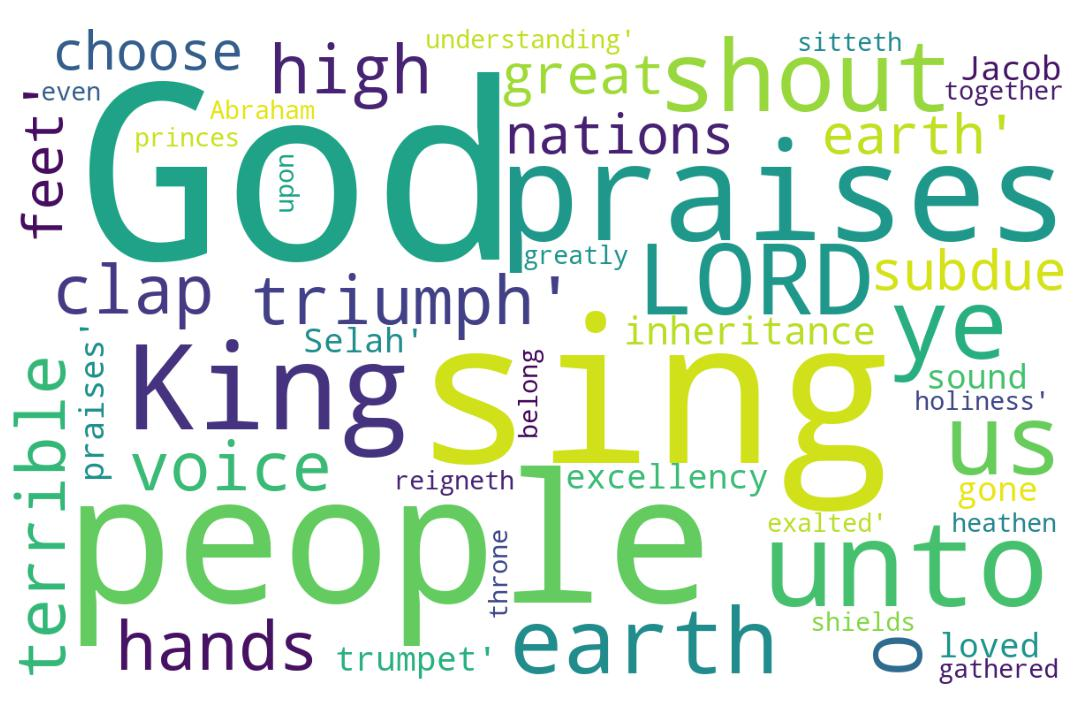
\includegraphics[width=\linewidth]{19OT-Psalms/Psalm47-WordCloud.jpg}
  \caption{Psalm 47 Word Cloud}
  \label{fig:Psalm 47 word Cloud}
\end{figure}

\marginpar{\scriptsize \centering \fcolorbox{bone}{lime}{\textbf{THE REIGNING KING}}\\ (Psalm 47:1-9) \begin{compactenum}[I.][8]
    \item The \textbf{Chronology} of end-time Events \index[scripture]{Psalms!Psa 044}\index[scripture]{Psalms!Psa 045}\index[scripture]{Psalms!Psa 046}\index[scripture]{Psalms!Psa 047} (Psa 44-47)
    \item The \textbf{Culmination} of History \index[scripture]{Psalms!Psa 047:02} (Psa 47:2)
    \item The \textbf{Command} of this King \index[scripture]{Psalms!Psa 047:02} (Psa 47:2)
    \item The \textbf{Conquests} of this King \index[scripture]{Psalms!Psa 047:03} (Psa 47:3)
    \item The \textbf{Concern} of this King \index[scripture]{Psalms!Psa 047:04} (Psa 47:4)
    \item The \textbf{Chorus} of Praise \index[scripture]{Psalms!Psa 047:06} (Psa 47:6)
    \item The \textbf{King} enthroned \index[scripture]{Psalms!Psa 047:07} (Psa 47:7)
\end{compactenum}}
    
%%%%%%%%%%%%%%%%%%%%%%%%%%%%%%
%%%%%%%%%%%%%%%%%%%%%%%%%%%%%%
\footnote{\textcolor[cmyk]{0.99998,1,0,0}{\hyperlink{TOC}{Return to end of Table of Contents.}}}\footnote{\href{https://audiobible.com/bible/psalms_47.html}{\textcolor[cmyk]{0.99998,1,0,0}{Psalms Audio}}}\textcolor[cmyk]{0.99998,1,0,0}{To the chief Musician, A Psalm for the sons of Korah.}\\
\\
\textcolor[cmyk]{0.99998,1,0,0}{O clap your hands, all ye people; shout unto God with the voice of triumph.}
[2] \textcolor[cmyk]{0.99998,1,0,0}{For the LORD most high \emph{is} terrible; \emph{he} \emph{is} a great King over all the earth.}\footnote{\textbf{Zechariah 14:9}  - And the LORD shall be king over all the earth: in that day shall there be one LORD, and his name one.}
[3] \textcolor[cmyk]{0.99998,1,0,0}{He shall subdue the people under us, and the nations under our feet.}\footnote{\textbf{Philippians 3:21} - Who shall change our vile body, that it may be fashioned like unto his glorious body, according to the working whereby he is able even to subdue all things unto himself.}
[4] \textcolor[cmyk]{0.99998,1,0,0}{He shall choose our inheritance for us, the excellency of Jacob whom he loved. Selah.}
[5] \textcolor[cmyk]{0.99998,1,0,0}{God is gone up with a shout, the LORD with the sound of a trumpet.}
[6] \textcolor[cmyk]{0.99998,1,0,0}{Sing praises to God, sing praises: sing praises unto our King, sing praises.}
[7] \textcolor[cmyk]{0.99998,1,0,0}{For God \emph{is} the King of all the earth: sing ye praises with \fcolorbox{bone}{MYGOLD}{understanding}.}
[8] \textcolor[cmyk]{0.99998,1,0,0}{God reigneth over the heathen: God sitteth upon the throne of his holiness.}
[9] \textcolor[cmyk]{0.99998,1,0,0}{The princes of the people are gathered together, \emph{even} the people of the God of Abraham: for the shields of the earth \emph{belong} unto God: he is greatly exalted.}\footnote{\textbf{Genesis 26:24} - And the LORD appeared unto him the same night, and said, I am the God of Abraham thy father: fear not, for I am with thee, and will bless thee, and multiply thy seed for my servant Abraham’s sake.}\footnote{\textbf{Exodus 3:6} - Moreover he said, I am the God of thy father, the God of Abraham, the God of Isaac, and the God of Jacob. And Moses hid his face; for he was afraid to look upon God.}\footnote{\textbf{Acts 7:32} - Saying, I am the God of thy fathers, the God of Abraham, and the God of Isaac, and the God of Jacob. Then Moses trembled, and durst not behold.}
\index[NWIV]{15!Psalms!Psa 47:1}\index[AWIP]{O!Psalms!Psa 47:1}\index[AWIP]{clap!Psalms!Psa 47:1}\index[AWIP]{your!Psalms!Psa 47:1}\index[AWIP]{hands!Psalms!Psa 47:1}\index[AWIP]{all!Psalms!Psa 47:1}\index[AWIP]{ye!Psalms!Psa 47:1}\index[AWIP]{people!Psalms!Psa 47:1}\index[AWIP]{shout!Psalms!Psa 47:1}\index[AWIP]{unto!Psalms!Psa 47:1}\index[AWIP]{God!Psalms!Psa 47:1}\index[AWIP]{with!Psalms!Psa 47:1}\index[AWIP]{the!Psalms!Psa 47:1}\index[AWIP]{voice!Psalms!Psa 47:1}\index[AWIP]{of!Psalms!Psa 47:1}\index[AWIP]{triumph!Psalms!Psa 47:1}

\index[NWIV]{16!Psalms!Psa 47:2}\index[AWIP]{For!Psalms!Psa 47:2}\index[AWIP]{the!Psalms!Psa 47:2}\index[AWIP]{the!Psalms!Psa 47:2 (2)}\index[AWIP]{LORD!Psalms!Psa 47:2}\index[AWIP]{most!Psalms!Psa 47:2}\index[AWIP]{high!Psalms!Psa 47:2}\index[AWIP]{\emph{is}!Psalms!Psa 47:2}\index[AWIP]{\emph{is}!Psalms!Psa 47:2 (2)}\index[AWIP]{terrible!Psalms!Psa 47:2}\index[AWIP]{\emph{he}!Psalms!Psa 47:2}\index[AWIP]{a!Psalms!Psa 47:2}\index[AWIP]{great!Psalms!Psa 47:2}\index[AWIP]{King!Psalms!Psa 47:2}\index[AWIP]{over!Psalms!Psa 47:2}\index[AWIP]{all!Psalms!Psa 47:2}\index[AWIP]{earth!Psalms!Psa 47:2}\index[AWIP]{\emph{is}!Psalms!Psa 47:2}\index[AWIP]{\emph{is}!Psalms!Psa 47:2 (2)}\index[AWIP]{\emph{he}!Psalms!Psa 47:2}

\index[NWIV]{13!Psalms!Psa 47:3}\index[AWIP]{He!Psalms!Psa 47:3}\index[AWIP]{shall!Psalms!Psa 47:3}\index[AWIP]{subdue!Psalms!Psa 47:3}\index[AWIP]{the!Psalms!Psa 47:3}\index[AWIP]{the!Psalms!Psa 47:3 (2)}\index[AWIP]{people!Psalms!Psa 47:3}\index[AWIP]{under!Psalms!Psa 47:3}\index[AWIP]{under!Psalms!Psa 47:3 (2)}\index[AWIP]{us!Psalms!Psa 47:3}\index[AWIP]{and!Psalms!Psa 47:3}\index[AWIP]{nations!Psalms!Psa 47:3}\index[AWIP]{our!Psalms!Psa 47:3}\index[AWIP]{feet!Psalms!Psa 47:3}

\index[NWIV]{15!Psalms!Psa 47:4}\index[AWIP]{He!Psalms!Psa 47:4}\index[AWIP]{shall!Psalms!Psa 47:4}\index[AWIP]{choose!Psalms!Psa 47:4}\index[AWIP]{our!Psalms!Psa 47:4}\index[AWIP]{inheritance!Psalms!Psa 47:4}\index[AWIP]{for!Psalms!Psa 47:4}\index[AWIP]{us!Psalms!Psa 47:4}\index[AWIP]{the!Psalms!Psa 47:4}\index[AWIP]{excellency!Psalms!Psa 47:4}\index[AWIP]{of!Psalms!Psa 47:4}\index[AWIP]{Jacob!Psalms!Psa 47:4}\index[AWIP]{whom!Psalms!Psa 47:4}\index[AWIP]{he!Psalms!Psa 47:4}\index[AWIP]{loved!Psalms!Psa 47:4}\index[AWIP]{Selah!Psalms!Psa 47:4}

\index[NWIV]{15!Psalms!Psa 47:5}\index[AWIP]{God!Psalms!Psa 47:5}\index[AWIP]{is!Psalms!Psa 47:5}\index[AWIP]{gone!Psalms!Psa 47:5}\index[AWIP]{up!Psalms!Psa 47:5}\index[AWIP]{with!Psalms!Psa 47:5}\index[AWIP]{with!Psalms!Psa 47:5 (2)}\index[AWIP]{a!Psalms!Psa 47:5}\index[AWIP]{a!Psalms!Psa 47:5 (2)}\index[AWIP]{shout!Psalms!Psa 47:5}\index[AWIP]{the!Psalms!Psa 47:5}\index[AWIP]{the!Psalms!Psa 47:5 (2)}\index[AWIP]{LORD!Psalms!Psa 47:5}\index[AWIP]{sound!Psalms!Psa 47:5}\index[AWIP]{of!Psalms!Psa 47:5}\index[AWIP]{trumpet!Psalms!Psa 47:5}

\index[NWIV]{13!Psalms!Psa 47:6}\index[AWIP]{Sing!Psalms!Psa 47:6}\index[AWIP]{praises!Psalms!Psa 47:6}\index[AWIP]{praises!Psalms!Psa 47:6 (2)}\index[AWIP]{praises!Psalms!Psa 47:6 (3)}\index[AWIP]{praises!Psalms!Psa 47:6 (4)}\index[AWIP]{to!Psalms!Psa 47:6}\index[AWIP]{God!Psalms!Psa 47:6}\index[AWIP]{sing!Psalms!Psa 47:6}\index[AWIP]{sing!Psalms!Psa 47:6 (2)}\index[AWIP]{sing!Psalms!Psa 47:6 (3)}\index[AWIP]{unto!Psalms!Psa 47:6}\index[AWIP]{our!Psalms!Psa 47:6}\index[AWIP]{King!Psalms!Psa 47:6}

\index[NWIV]{14!Psalms!Psa 47:7}\index[AWIP]{For!Psalms!Psa 47:7}\index[AWIP]{God!Psalms!Psa 47:7}\index[AWIP]{\emph{is}!Psalms!Psa 47:7}\index[AWIP]{the!Psalms!Psa 47:7}\index[AWIP]{the!Psalms!Psa 47:7 (2)}\index[AWIP]{King!Psalms!Psa 47:7}\index[AWIP]{of!Psalms!Psa 47:7}\index[AWIP]{all!Psalms!Psa 47:7}\index[AWIP]{earth!Psalms!Psa 47:7}\index[AWIP]{sing!Psalms!Psa 47:7}\index[AWIP]{ye!Psalms!Psa 47:7}\index[AWIP]{praises!Psalms!Psa 47:7}\index[AWIP]{with!Psalms!Psa 47:7}\index[AWIP]{understanding!Psalms!Psa 47:7}\index[AWIP]{\emph{is}!Psalms!Psa 47:7}

\index[NWIV]{13!Psalms!Psa 47:8}\index[AWIP]{God!Psalms!Psa 47:8}\index[AWIP]{God!Psalms!Psa 47:8 (2)}\index[AWIP]{reigneth!Psalms!Psa 47:8}\index[AWIP]{over!Psalms!Psa 47:8}\index[AWIP]{the!Psalms!Psa 47:8}\index[AWIP]{the!Psalms!Psa 47:8 (2)}\index[AWIP]{heathen!Psalms!Psa 47:8}\index[AWIP]{sitteth!Psalms!Psa 47:8}\index[AWIP]{upon!Psalms!Psa 47:8}\index[AWIP]{throne!Psalms!Psa 47:8}\index[AWIP]{of!Psalms!Psa 47:8}\index[AWIP]{his!Psalms!Psa 47:8}\index[AWIP]{holiness!Psalms!Psa 47:8}

\index[NWIV]{29!Psalms!Psa 47:9}\index[AWIP]{The!Psalms!Psa 47:9}\index[AWIP]{princes!Psalms!Psa 47:9}\index[AWIP]{of!Psalms!Psa 47:9}\index[AWIP]{of!Psalms!Psa 47:9 (2)}\index[AWIP]{of!Psalms!Psa 47:9 (3)}\index[AWIP]{of!Psalms!Psa 47:9 (4)}\index[AWIP]{the!Psalms!Psa 47:9}\index[AWIP]{the!Psalms!Psa 47:9 (2)}\index[AWIP]{the!Psalms!Psa 47:9 (3)}\index[AWIP]{the!Psalms!Psa 47:9 (4)}\index[AWIP]{the!Psalms!Psa 47:9 (5)}\index[AWIP]{people!Psalms!Psa 47:9}\index[AWIP]{people!Psalms!Psa 47:9 (2)}\index[AWIP]{are!Psalms!Psa 47:9}\index[AWIP]{gathered!Psalms!Psa 47:9}\index[AWIP]{together!Psalms!Psa 47:9}\index[AWIP]{\emph{even}!Psalms!Psa 47:9}\index[AWIP]{God!Psalms!Psa 47:9}\index[AWIP]{God!Psalms!Psa 47:9 (2)}\index[AWIP]{Abraham!Psalms!Psa 47:9}\index[AWIP]{for!Psalms!Psa 47:9}\index[AWIP]{shields!Psalms!Psa 47:9}\index[AWIP]{earth!Psalms!Psa 47:9}\index[AWIP]{\emph{belong}!Psalms!Psa 47:9}\index[AWIP]{unto!Psalms!Psa 47:9}\index[AWIP]{he!Psalms!Psa 47:9}\index[AWIP]{is!Psalms!Psa 47:9}\index[AWIP]{greatly!Psalms!Psa 47:9}\index[AWIP]{exalted!Psalms!Psa 47:9}\index[AWIP]{\emph{even}!Psalms!Psa 47:9}\index[AWIP]{\emph{belong}!Psalms!Psa 47:9}


\section{Psalm 47 Outlines}

\subsection{My Outlines}

\subsubsection{The Reigning King}

\index[speaker]{Keith Anthony!Psalm 047 (The Reigning King)}
\index[series]{Psalms (Keith Anthony)!Psalm 047 (The Reigning King)}
\index[date]{2016/07/22!Psalm 047 (The Reigning King) (Keith Anthony)}

\begin{compactenum}[I.][8]
    \item The \textbf{Chronology} of end-time Events \index[scripture]{Psalms!Psa 044}\index[scripture]{Psalms!Psa 045}\index[scripture]{Psalms!Psa 046}\index[scripture]{Psalms!Psa 047} (Psa 44-47)
    \item The \textbf{Culmination} of History \index[scripture]{Psalms!Psa 047:02} (Psa 47:2)
    \item The \textbf{Command} of this King \index[scripture]{Psalms!Psa 047:02} (Psa 47:2)
    \item The \textbf{Conquests} of this King \index[scripture]{Psalms!Psa 047:03} (Psa 47:3)
    \item The \textbf{Concern} of this King \index[scripture]{Psalms!Psa 047:04} (Psa 47:4)
    \item The \textbf{Chorus} of Praise \index[scripture]{Psalms!Psa 047:06} (Psa 47:6)
    \item The \textbf{King} enthroned \index[scripture]{Psalms!Psa 047:07} (Psa 47:7)
\end{compactenum}


\subsection{Outlines from Others}

\section{Psalm 47 Comments}

\subsection{Numeric Nuggets}
Verses 3, 6, and 8 have 13 words. The 13-letter word ``understanding'' is used in the psalm. the 13$^{th}$ word in the chapter is the word ``voice.''

\subsection{Psalm 47 Introduction}
Psalm 44 through 47 are arranged in chronological and prophetic order.
\begin{compactenum}
	\item Psalm 44 concerns the Great Tribulation
	\item Psalm 45 covers the Marriage of the Lamb
	\item Psalm 46 concerns the Second Advent, and
	\item Psalm 47 concerns the Millennium and the Lord's reign therein.\\
\end{compactenum}

\noindent This is a similar arrangement as Psalm 21 through 23, which covers three separate roles (and time periods) of Jesus Christ.

\subsection{Psalm 47:1}
The New Testament believer can use the voice of triumph because of the triumph provided to us in Christ.\footnote{\textbf{2 Corinthians 2:14} - Now thanks be unto God, which always causeth us to triumph in Christ, and maketh manifest the savour of his knowledge by us in every place.} But this specific triumph is for the Lord reigning over the Earth (as described in verses 2 and 3).

\subsection{Psalm 47:5}
The sound of a trumpet is a trump, defined in 1 Corinthians 15:32 and 1 Thessalonians 4:16.

\subsection{Psalm 47:6}
The admonition to ``sing praises'' is found 4 times in the verse.  It is only found in the Old Testament, 18 times in total, one in 2 Samuel 22:50. All the other occurrences (17) are in 14 verses in 13 chapters in Psalms.
\subsection{Psalm 47 Repeated Phrases}


%%%%%%%%%%
%%%%%%%%%%
\normalsize
 
\begin{center}
\begin{longtable}{|c|c|}
\caption[Psalm 47 Repeated Phrases]{Psalm 47 Repeated Phrases}\label{table:Repeated Phrases Psalm 47} \\
\hline \multicolumn{1}{|c|}{\textbf{Phrase}} & \multicolumn{1}{c|}{\textbf{Frequency}} \\ \hline 
\endfirsthead
 
\multicolumn{2}{c}
{{\bfseries \tablename\ \thetable{} -- continued from previous page}} \\  
\hline \multicolumn{1}{|c|}{\textbf{Phrase}} & \multicolumn{1}{c|}{\textbf{Frequency}} \\ \hline 
\endhead
 
\hline \multicolumn{2}{c}{{ }} \\ \hline
\endfoot 
the earth & 3\\ \hline 
the people & 3\\ \hline 
sing praises & 3\\ \hline 
of the & 3\\ \hline 
\end{longtable}
\end{center}



%%%%%%%%%%
%%%%%%%%%%



\section{Psalm 47 Statistics}

%%%%%%%%%%%%%%%%%%%%%%%%%%%
%%%%% Word Statistics
%%%%%%%%%%%%%%%%%%%%%%%%%%


\normalsize



\subsection{Chapter Word Statistics}


%%%%%%%%%%
%%%%%%%%%%
 
\begin{center}
\begin{longtable}{l|c|c|c|c}
\caption[Stats for Psalm 47]{Stats for Psalm 47} \label{table:Stats for Psalm 47} \\ 
\hline \multicolumn{1}{|c|}{\textbf{Verse(s)}} & \multicolumn{1}{|c|}{\textbf{Count}} & \multicolumn{1}{|c|}{\textbf{Unique}} & \multicolumn{1}{|c|}{\textbf{Italics}} & \multicolumn{1}{|c|}{\textbf{Uniq Italic}}  \\ \hline 
\endfirsthead
 
\multicolumn{5}{c}
{{\bfseries \tablename\ \thetable{} -- continued from previous page}} \\  
\hline \multicolumn{1}{|c|}{\textbf{Verse(s)}} & \multicolumn{1}{|c|}{\textbf{Count}} & \multicolumn{1}{|c|}{\textbf{Unique}} & \multicolumn{1}{|c|}{\textbf{Italics}} & \multicolumn{1}{|c|}{\textbf{Uniq Italic}}  \\ \hline 
\endhead
 
\hline \multicolumn{5}{|r|}{{Continued if needed}} \\ \hline
\endfoot 
1 & 15 & 15 & 0 & 0\\ \hline
2 & 16 & 14 & 3 & 2\\ \hline
3 & 13 & 11 & 0 & 0\\ \hline
4 & 15 & 15 & 0 & 0\\ \hline
5 & 15 & 12 & 0 & 0\\ \hline
6 & 13 & 8 & 0 & 0\\ \hline
7 & 14 & 13 & 1 & 1\\ \hline
8 & 13 & 11 & 0 & 0\\ \hline
9 & 29 & 20 & 2 & 2\\ \hline
\hline \hline
Total & 143 & 73 & 6 & 4



\end{longtable}
\end{center}

%%%%%%%%%%
%%%%%%%%%%
 
\subsection{Words by Frequency}

\begin{center}
\begin{longtable}{l|r}
\caption[Word Frequencies in Psalm 47]{Word Frequencies in Psalm 47} \label{table:WordsIn-Psalm-47} \\ 
\hline \multicolumn{1}{|c|}{\textbf{Word}} & \multicolumn{1}{c|}{\textbf{Frequency}} \\ \hline 
\endfirsthead
 
\multicolumn{2}{c}
{{\bfseries \tablename\ \thetable{} -- continued from previous page}} \\ 
\hline \multicolumn{1}{|c|}{\textbf{Word}} & \multicolumn{1}{c|}{\textbf{Frequency}} \\ \hline 
\endhead
 
\hline \multicolumn{2}{|r|}{{Continued if needed}} \\ \hline
\endfoot
 
\hline \hline
\endlastfoot
the & 17 \\ \hline
of & 9 \\ \hline
God & 8 \\ \hline
praises & 5 \\ \hline
people & 4 \\ \hline
with & 4 \\ \hline
sing & 4 \\ \hline
all & 3 \\ \hline
unto & 3 \\ \hline
\emph{is} & 3 \\ \hline
a & 3 \\ \hline
King & 3 \\ \hline
earth & 3 \\ \hline
our & 3 \\ \hline
ye & 2 \\ \hline
shout & 2 \\ \hline
For & 2 \\ \hline
LORD & 2 \\ \hline
over & 2 \\ \hline
He & 2 \\ \hline
shall & 2 \\ \hline
under & 2 \\ \hline
us & 2 \\ \hline
for & 2 \\ \hline
he & 2 \\ \hline
is & 2 \\ \hline
O & 1 \\ \hline
clap & 1 \\ \hline
your & 1 \\ \hline
hands & 1 \\ \hline
voice & 1 \\ \hline
triumph & 1 \\ \hline
most & 1 \\ \hline
high & 1 \\ \hline
terrible & 1 \\ \hline
\emph{he} & 1 \\ \hline
great & 1 \\ \hline
subdue & 1 \\ \hline
and & 1 \\ \hline
nations & 1 \\ \hline
feet & 1 \\ \hline
choose & 1 \\ \hline
inheritance & 1 \\ \hline
excellency & 1 \\ \hline
Jacob & 1 \\ \hline
whom & 1 \\ \hline
loved & 1 \\ \hline
Selah & 1 \\ \hline
gone & 1 \\ \hline
up & 1 \\ \hline
sound & 1 \\ \hline
trumpet & 1 \\ \hline
Sing & 1 \\ \hline
to & 1 \\ \hline
understanding & 1 \\ \hline
reigneth & 1 \\ \hline
heathen & 1 \\ \hline
sitteth & 1 \\ \hline
upon & 1 \\ \hline
throne & 1 \\ \hline
his & 1 \\ \hline
holiness & 1 \\ \hline
The & 1 \\ \hline
princes & 1 \\ \hline
are & 1 \\ \hline
gathered & 1 \\ \hline
together & 1 \\ \hline
\emph{even} & 1 \\ \hline
Abraham & 1 \\ \hline
shields & 1 \\ \hline
\emph{belong} & 1 \\ \hline
greatly & 1 \\ \hline
exalted & 1 \\ \hline
\end{longtable}
\end{center}



\normalsize



\subsection{Words Alphabetically}

\begin{center}
\begin{longtable}{l|r}
\caption[Word Alphabetically in Psalm 47]{Word Alphabetically in Psalm 47} \label{table:WordsIn-Psalm-47} \\ 
\hline \multicolumn{1}{|c|}{\textbf{Word}} & \multicolumn{1}{c|}{\textbf{Frequency}} \\ \hline 
\endfirsthead
 
\multicolumn{2}{c}
{{\bfseries \tablename\ \thetable{} -- continued from previous page}} \\ 
\hline \multicolumn{1}{|c|}{\textbf{Word}} & \multicolumn{1}{c|}{\textbf{Frequency}} \\ \hline 
\endhead
 
\hline \multicolumn{2}{|r|}{{Continued if needed}} \\ \hline
\endfoot
 
\hline \hline
\endlastfoot
Abraham & 1 \\ \hline
For & 2 \\ \hline
God & 8 \\ \hline
He & 2 \\ \hline
Jacob & 1 \\ \hline
King & 3 \\ \hline
LORD & 2 \\ \hline
O & 1 \\ \hline
Selah & 1 \\ \hline
Sing & 1 \\ \hline
The & 1 \\ \hline
\emph{belong} & 1 \\ \hline
\emph{even} & 1 \\ \hline
\emph{he} & 1 \\ \hline
\emph{is} & 3 \\ \hline
a & 3 \\ \hline
all & 3 \\ \hline
and & 1 \\ \hline
are & 1 \\ \hline
choose & 1 \\ \hline
clap & 1 \\ \hline
earth & 3 \\ \hline
exalted & 1 \\ \hline
excellency & 1 \\ \hline
feet & 1 \\ \hline
for & 2 \\ \hline
gathered & 1 \\ \hline
gone & 1 \\ \hline
great & 1 \\ \hline
greatly & 1 \\ \hline
hands & 1 \\ \hline
he & 2 \\ \hline
heathen & 1 \\ \hline
high & 1 \\ \hline
his & 1 \\ \hline
holiness & 1 \\ \hline
inheritance & 1 \\ \hline
is & 2 \\ \hline
loved & 1 \\ \hline
most & 1 \\ \hline
nations & 1 \\ \hline
of & 9 \\ \hline
our & 3 \\ \hline
over & 2 \\ \hline
people & 4 \\ \hline
praises & 5 \\ \hline
princes & 1 \\ \hline
reigneth & 1 \\ \hline
shall & 2 \\ \hline
shields & 1 \\ \hline
shout & 2 \\ \hline
sing & 4 \\ \hline
sitteth & 1 \\ \hline
sound & 1 \\ \hline
subdue & 1 \\ \hline
terrible & 1 \\ \hline
the & 17 \\ \hline
throne & 1 \\ \hline
to & 1 \\ \hline
together & 1 \\ \hline
triumph & 1 \\ \hline
trumpet & 1 \\ \hline
under & 2 \\ \hline
understanding & 1 \\ \hline
unto & 3 \\ \hline
up & 1 \\ \hline
upon & 1 \\ \hline
us & 2 \\ \hline
voice & 1 \\ \hline
whom & 1 \\ \hline
with & 4 \\ \hline
ye & 2 \\ \hline
your & 1 \\ \hline
\end{longtable}
\end{center}



\normalsize



\subsection{Word Lengths in Chapter}
\normalsize
\begin{longtable}{l|p{3.75in}}
\caption[Words by Length in Psalm 47]{Words by Length in Psalm 47} \label{table:WordsIn-Psalm-47} \\ 
\hline \multicolumn{1}{|c|}{\textbf{Length}} & \multicolumn{1}{c|}{\textbf{Words}} \\ \hline 
\endfirsthead
 
\multicolumn{2}{c}
{{\bfseries \tablename\ \thetable{} -- continued from previous page}} \\ 
\hline \multicolumn{1}{|c|}{\textbf{Length}} & \multicolumn{1}{c|}{\textbf{Words}} \\ \hline 
\endhead
 
\hline \multicolumn{2}{|r|}{{Continued if needed}} \\ \hline
\endfoot
 
\hline \hline
\endlastfoot
1 & O, a \\ \hline
2 & ye, of, \emph{is}, \emph{he}, He, us, he, is, up, to \\ \hline
3 & all, God, the, For, and, our, for, his, The, are \\ \hline
4 & clap, your, unto, with, LORD, most, high, King, over, feet, whom, gone, Sing, sing, upon, \emph{even} \\ \hline
5 & hands, shout, voice, great, earth, shall, under, Jacob, loved, Selah, sound \\ \hline
6 & people, subdue, choose, throne, \emph{belong} \\ \hline
7 & triumph, nations, trumpet, praises, heathen, sitteth, princes, Abraham, shields, greatly, exalted \\ \hline
8 & terrible, reigneth, holiness, gathered, together \\ \hline
10 & excellency \\ \hline
11 & inheritance \\ \hline
13 & understanding \\ \hline
\end{longtable}






%%%%%%%%%%
%%%%%%%%%%
 



%%%%%%%%%%
%%%%%%%%%%
\subsection{Verses with 13 Words in Chapter}
\normalsize
\begin{longtable}{l|p{3.75in}}
\caption[Verses with 13 Words  in Psalm 47]{Verses with 13 Words  in Psalm 47} \label{table:Verses with 13 Words in-Psalm-47} \\ 
\hline \multicolumn{1}{|c|}{\textbf{Reference}} & \multicolumn{1}{c|}{\textbf{Verse}} \\ \hline 
\endfirsthead
 
\multicolumn{2}{c}
{{\bfseries \tablename\ \thetable{} -- continued from previous page}} \\ 
\hline \multicolumn{1}{|c|}{\textbf{Reference}} & \multicolumn{1}{c|}{\textbf{Verse}} \\ \hline 
\endhead
 
\hline \multicolumn{2}{|r|}{{Continued if needed}} \\ \hline
\endfoot
 
\hline \hline
\endlastfoot
Psalms 047:3 & He shall subdue the people under us, and the nations under our feet. \\ \hline
Psalms 047:6 & Sing praises to God, sing praises: sing praises unto our King, sing praises. \\ \hline
Psalms 047:8 & God reigneth over the heathen: God sitteth upon the throne of his holiness. \\ \hline
\end{longtable}






%%%%%%%%%%
%%%%%%%%%%

 \chapter{Proverb 16}
 
\begin{figure}
  \includegraphics[width=\linewidth]{20OT-Proverbs/Proverb16-Wordcloud.jpg}
  \caption{Proverb 16 Word Cloud}
  \label{fig:Proverb 16 word Cloud}
\end{figure}

\marginpar{\scriptsize \centering \fcolorbox{bone}{lime}{\textbf{PRAYERS FOR THE FAITHFUL}}\\ (Proverb 16:1-33) \begin{compactenum}[I.][8]
    \item \textbf{Prepare my Heart}  \index[scripture]{Proverbs!Pro 16:01}(Pro 16:1)
    \item \textbf{Peruse my Ways} \index[scripture]{Proverbs!Pro 16:02}(Pro 16:2)
    \item \textbf{Purify my Thoughts} \index[scripture]{Proverbs!Pro 16:03}(Pro 16:3)
    \item \textbf{Point out the Path} \index[scripture]{Proverbs!Pro 16:09}(Pro 16:9)
    \item \textbf{Passify my Anger} \index[scripture]{Proverbs!Pro 16:14}(Pro 16:14)
    \item \textbf{Preserve my Soul} \index[scripture]{Proverbs!Pro 16:17}(Pro 16:17)
    \item \textbf{Impart Wisdom} \index[scripture]{Proverbs!Pro 16:21}(Pro 16:21)
\end{compactenum}}

\marginpar{\scriptsize \centering \fcolorbox{bone}{yellow}{\textbf{A GODLY MAN}}\\ (Proverb 16:1-33) \begin{compactenum}[I.][8]
    \item Is \textbf{Prepared}  \index[scripture]{Proverbs!Pro 16:01} (Pro 16:1)
    \item Is \textbf{Purposed}  \index[scripture]{Proverbs!Pro 16:03} (Pro 16:3)
    \item Has \textbf{Purged} Iniquity  \index[scripture]{Proverbs!Pro 16:06} (Pro 16:6)
    \item Is \textbf{Peaceable}   \index[scripture]{Proverbs!Pro 16:07} (Pro 16:7)
    \item Is \textbf{Preserved}   \index[scripture]{Proverbs!Pro 16:17} (Pro 16:17)
    \item Is not \textbf{Proud}   \index[scripture]{Proverbs!Pro 16:19} (Pro 16:19)
    \item Is \textbf{Prudent}   \index[scripture]{Proverbs!Pro 16:21} (Pro 16:21)
\end{compactenum}}

\marginpar{\scriptsize \centering \fcolorbox{bone}{black}{\textbf{\textcolor[cmyk]{0,0,0,0}{GOD IN CONTROL}}}\\ (Proverb 16) 
 \begin{compactenum}[I.][8]
	\item \textbf{Determined Spirits} \index[scripture]{Proverbs!Pro 16:09} (Pro 16:9)
	\item \textbf{Directed Steps}  \index[scripture]{Proverbs!Pro 16:09} (Pro 16:9)
	\item A \textbf{Divine Sentence}  \index[scripture]{Proverbs!Pro 16:10}  (Pro 16:10)
	\item \textbf{Destroyed Soul}  \index[scripture]{Proverbs!Pro 16:18}  (Pro 16:18)
	\item A \textbf{Delighted Soul}  \index[scripture]{Proverbs!Pro 16:19}  (Pro 16:19)
	\item \textbf{Dug-up Sorrows}  \index[scripture]{Proverbs!Pro 16:27} (Pro 16:27)
	\item A \textbf{Disciplined Spirit}  \index[scripture]{Proverbs!Pro 16:32} (Pro 16:32)
\end{compactenum}}

\footnote{\textcolor[cmyk]{0.99998,1,0,0}{\hyperlink{TOC}{Return to end of Table of Contents.}}}\footnote{\href{https://audiobible.com/bible/proverbs_16.html}{\textcolor[cmyk]{0.99998,1,0,0}{Proverbs Audio}}}\textcolor[cmyk]{0.99998,1,0,0}{The \fcolorbox{bone}{lime}{preparations of the heart} in man, and the answer of the tongue, \emph{is} from the LORD.}
[2] \textcolor[cmyk]{0.99998,1,0,0}{All the ways of a man \emph{are} clean in his own eyes; but the \fcolorbox{bone}{lime}{LORD} \fcolorbox{bone}{lime}{weigheth} \fcolorbox{bone}{lime}{the} \fcolorbox{bone}{lime}{spirits}.}
[3] \textcolor[cmyk]{0.99998,1,0,0}{Commit thy works unto the LORD, and thy \fcolorbox{bone}{lime}{thoughts shall be} \fcolorbox{bone}{lime}{established}.}
[4] \textcolor[cmyk]{0.99998,1,0,0}{The LORD hath made all \emph{things} for himself: yea, even the wicked for the day of evil.}
[5] \textcolor[cmyk]{0.99998,1,0,0}{Every one \emph{that} \emph{is} proud in heart \emph{is} an abomination to the LORD: \emph{though} hand \emph{join} in hand, he shall not be unpunished.}
[6] \textcolor[cmyk]{0.99998,1,0,0}{By mercy and truth iniquity is purged: and by the fear of the LORD \emph{men} depart from evil.}
[7] \textcolor[cmyk]{0.99998,1,0,0}{When a man's ways please the LORD, he maketh even his enemies to be at peace with him.}
[8] \textcolor[cmyk]{0.99998,1,0,0}{Better \emph{is} a little with \fcolorbox{bone}{MYGOLD}{righteousness} than great revenues without right.}
[9] \textcolor[cmyk]{0.99998,1,0,0}{A man's heart deviseth his way: but the \fcolorbox{bone}{lime}{LORD directeth his steps}.}
[10] \textcolor[cmyk]{0.99998,1,0,0}{A divine sentence \emph{is} in the lips of the king: his mouth \fcolorbox{bone}{MYGOLD}{transgresseth} not in judgment.}
[11] \textcolor[cmyk]{0.99998,1,0,0}{A just weight and balance \emph{are} the LORD'S: all the weights of the bag \emph{are} his work.}
[12] \textcolor[cmyk]{0.99998,1,0,0}{\emph{It} \emph{is} an abomination to kings to commit wickedness: for the throne is established by \fcolorbox{bone}{MYGOLD}{righteousness}.}
[13] \textcolor[cmyk]{0.99998,1,0,0}{Righteous lips \emph{are} the delight of kings; and they love him that speaketh right.}
[14] \textcolor[cmyk]{0.99998,1,0,0}{The wrath of a king \emph{is} \emph{as} messengers of death: but a \fcolorbox{bone}{lime}{wise man will pacify it}.}
[15] \textcolor[cmyk]{0.99998,1,0,0}{In the light of the king's countenance \emph{is} life; and his favour \emph{is} as a cloud of the latter rain.}
[16] \textcolor[cmyk]{0.99998,1,0,0}{How much better \emph{is} \emph{it} to get wisdom than gold! and to get \fcolorbox{bone}{MYGOLD}{understanding} rather to be chosen than silver!}
[17] \textcolor[cmyk]{0.99998,1,0,0}{The highway of the upright \emph{is} to depart from evil: he that keepeth his way \fcolorbox{bone}{lime}{preserveth} his soul.}
[18] \textcolor[cmyk]{0.99998,1,0,0}{Pride \emph{goeth} before destruction, and an haughty spirit before a fall.}
[19] \textcolor[cmyk]{0.99998,1,0,0}{Better \emph{it} \emph{is} \emph{to} \emph{be} of an humble spirit with the lowly, than to divide the spoil with the proud.}
[20] \textcolor[cmyk]{0.99998,1,0,0}{He that handleth a matter wisely shall find good: and whoso trusteth in the LORD, happy \emph{is} he.}
[21] \textcolor[cmyk]{0.99998,1,0,0}{The \fcolorbox{bone}{lime}{wise in heart} shall be called prudent: and the sweetness of the lips increaseth learning.}
[22] \textcolor[cmyk]{0.99998,1,0,0}{\fcolorbox{bone}{MYGOLD}{Understanding} \emph{is} a wellspring of life unto him that hath it: but the instruction of fools \emph{is} folly.}\footnote{\textbf{Proverbs 18:4} - The words of a man’s mouth are as deep waters, and the wellspring of wisdom as a flowing brook.}\marginpar{ \scriptsize  {\textcolor[rgb]{0.00,0.545,0.269}{$\rightarrow$``wellspring'' found ONLY here and in Proverbs 18:4.}}}
[23] \textcolor[cmyk]{0.99998,1,0,0}{The heart of the wise teacheth his mouth, and addeth learning to his lips.}
[24] \textcolor[cmyk]{0.99998,1,0,0}{Pleasant words \emph{are} \emph{as} an honeycomb, sweet to the soul, and health to the bones.}
[25] \textcolor[cmyk]{0.99998,1,0,0}{There is a way that seemeth right unto a man, but the end thereof \emph{are} the ways of death.}
[26] \textcolor[cmyk]{0.99998,1,0,0}{He that laboureth laboureth for himself; for his mouth craveth it of him.}
[27] \textcolor[cmyk]{0.99998,1,0,0}{An ungodly man diggeth up evil: and in his lips \emph{there} \emph{is} as a burning fire.}
[28] \textcolor[cmyk]{0.99998,1,0,0}{A froward man soweth strife: and a whisperer separateth chief friends.}\footnote{\textbf{Proverb 6:14} - Frowardness is in his heart, he deviseth mischief continually; he soweth discord.}\footnote{\textbf{Proverb 6:19} - A false witness that speaketh lies, and he that soweth discord among brethren.}
[29] \textcolor[cmyk]{0.99998,1,0,0}{A violent man enticeth his neighbour, and leadeth him into the way \emph{that} \emph{is} not good.}
[30] \textcolor[cmyk]{0.99998,1,0,0}{He shutteth his eyes to devise froward things: moving his lips he bringeth evil to pass.}
[31] \textcolor[cmyk]{0.99998,1,0,0}{The hoary head \emph{is} a crown of glory, \emph{if} it be found in the way of \fcolorbox{bone}{MYGOLD}{righteousness}.}
[32] \textcolor[cmyk]{0.99998,1,0,0}{\emph{He} \emph{that} \emph{is} slow to anger \emph{is} better than the mighty; and he that ruleth his spirit than he that taketh a city.}
[33] \textcolor[cmyk]{0.99998,1,0,0}{The lot is cast into the lap; but the whole disposing thereof \emph{is} of the LORD.}



\index[NWIV]{17!Proverbs!Pro 16:1}\index[AWIP]{The!Proverbs!Pro 16:1}\index[AWIP]{preparations!Proverbs!Pro 16:1}\index[AWIP]{of!Proverbs!Pro 16:1}\index[AWIP]{of!Proverbs!Pro 16:1 (2)}\index[AWIP]{the!Proverbs!Pro 16:1}\index[AWIP]{the!Proverbs!Pro 16:1 (2)}\index[AWIP]{the!Proverbs!Pro 16:1 (3)}\index[AWIP]{the!Proverbs!Pro 16:1 (4)}\index[AWIP]{heart!Proverbs!Pro 16:1}\index[AWIP]{in!Proverbs!Pro 16:1}\index[AWIP]{man!Proverbs!Pro 16:1}\index[AWIP]{and!Proverbs!Pro 16:1}\index[AWIP]{answer!Proverbs!Pro 16:1}\index[AWIP]{tongue!Proverbs!Pro 16:1}\index[AWIP]{\emph{is}!Proverbs!Pro 16:1}\index[AWIP]{from!Proverbs!Pro 16:1}\index[AWIP]{LORD!Proverbs!Pro 16:1}\index[AWIP]{\emph{is}!Proverbs!Pro 16:1}

\index[NWIV]{18!Proverbs!Pro 16:2}\index[AWIP]{All!Proverbs!Pro 16:2}\index[AWIP]{the!Proverbs!Pro 16:2}\index[AWIP]{the!Proverbs!Pro 16:2 (2)}\index[AWIP]{the!Proverbs!Pro 16:2 (3)}\index[AWIP]{ways!Proverbs!Pro 16:2}\index[AWIP]{of!Proverbs!Pro 16:2}\index[AWIP]{a!Proverbs!Pro 16:2}\index[AWIP]{man!Proverbs!Pro 16:2}\index[AWIP]{\emph{are}!Proverbs!Pro 16:2}\index[AWIP]{clean!Proverbs!Pro 16:2}\index[AWIP]{in!Proverbs!Pro 16:2}\index[AWIP]{his!Proverbs!Pro 16:2}\index[AWIP]{own!Proverbs!Pro 16:2}\index[AWIP]{eyes!Proverbs!Pro 16:2}\index[AWIP]{but!Proverbs!Pro 16:2}\index[AWIP]{LORD!Proverbs!Pro 16:2}\index[AWIP]{weigheth!Proverbs!Pro 16:2}\index[AWIP]{spirits!Proverbs!Pro 16:2}\index[AWIP]{\emph{are}!Proverbs!Pro 16:2}

\index[NWIV]{12!Proverbs!Pro 16:3}\index[AWIP]{Commit!Proverbs!Pro 16:3}\index[AWIP]{thy!Proverbs!Pro 16:3}\index[AWIP]{thy!Proverbs!Pro 16:3 (2)}\index[AWIP]{works!Proverbs!Pro 16:3}\index[AWIP]{unto!Proverbs!Pro 16:3}\index[AWIP]{the!Proverbs!Pro 16:3}\index[AWIP]{LORD!Proverbs!Pro 16:3}\index[AWIP]{and!Proverbs!Pro 16:3}\index[AWIP]{thoughts!Proverbs!Pro 16:3}\index[AWIP]{shall!Proverbs!Pro 16:3}\index[AWIP]{be!Proverbs!Pro 16:3}\index[AWIP]{established!Proverbs!Pro 16:3}

\index[NWIV]{17!Proverbs!Pro 16:4}\index[AWIP]{The!Proverbs!Pro 16:4}\index[AWIP]{LORD!Proverbs!Pro 16:4}\index[AWIP]{hath!Proverbs!Pro 16:4}\index[AWIP]{made!Proverbs!Pro 16:4}\index[AWIP]{all!Proverbs!Pro 16:4}\index[AWIP]{\emph{things}!Proverbs!Pro 16:4}\index[AWIP]{for!Proverbs!Pro 16:4}\index[AWIP]{for!Proverbs!Pro 16:4 (2)}\index[AWIP]{himself!Proverbs!Pro 16:4}\index[AWIP]{yea!Proverbs!Pro 16:4}\index[AWIP]{even!Proverbs!Pro 16:4}\index[AWIP]{the!Proverbs!Pro 16:4}\index[AWIP]{the!Proverbs!Pro 16:4 (2)}\index[AWIP]{wicked!Proverbs!Pro 16:4}\index[AWIP]{day!Proverbs!Pro 16:4}\index[AWIP]{of!Proverbs!Pro 16:4}\index[AWIP]{evil!Proverbs!Pro 16:4}\index[AWIP]{\emph{things}!Proverbs!Pro 16:4}

\index[NWIV]{23!Proverbs!Pro 16:5}\index[AWIP]{Every!Proverbs!Pro 16:5}\index[AWIP]{one!Proverbs!Pro 16:5}\index[AWIP]{\emph{that}!Proverbs!Pro 16:5}\index[AWIP]{\emph{is}!Proverbs!Pro 16:5}\index[AWIP]{\emph{is}!Proverbs!Pro 16:5 (2)}\index[AWIP]{proud!Proverbs!Pro 16:5}\index[AWIP]{in!Proverbs!Pro 16:5}\index[AWIP]{in!Proverbs!Pro 16:5 (2)}\index[AWIP]{heart!Proverbs!Pro 16:5}\index[AWIP]{an!Proverbs!Pro 16:5}\index[AWIP]{abomination!Proverbs!Pro 16:5}\index[AWIP]{to!Proverbs!Pro 16:5}\index[AWIP]{the!Proverbs!Pro 16:5}\index[AWIP]{LORD!Proverbs!Pro 16:5}\index[AWIP]{\emph{though}!Proverbs!Pro 16:5}\index[AWIP]{hand!Proverbs!Pro 16:5}\index[AWIP]{hand!Proverbs!Pro 16:5 (2)}\index[AWIP]{\emph{join}!Proverbs!Pro 16:5}\index[AWIP]{he!Proverbs!Pro 16:5}\index[AWIP]{shall!Proverbs!Pro 16:5}\index[AWIP]{not!Proverbs!Pro 16:5}\index[AWIP]{be!Proverbs!Pro 16:5}\index[AWIP]{unpunished!Proverbs!Pro 16:5}\index[AWIP]{\emph{that}!Proverbs!Pro 16:5}\index[AWIP]{\emph{is}!Proverbs!Pro 16:5}\index[AWIP]{\emph{is}!Proverbs!Pro 16:5 (2)}\index[AWIP]{\emph{though}!Proverbs!Pro 16:5}\index[AWIP]{\emph{join}!Proverbs!Pro 16:5}

\index[NWIV]{18!Proverbs!Pro 16:6}\index[AWIP]{By!Proverbs!Pro 16:6}\index[AWIP]{mercy!Proverbs!Pro 16:6}\index[AWIP]{and!Proverbs!Pro 16:6}\index[AWIP]{and!Proverbs!Pro 16:6 (2)}\index[AWIP]{truth!Proverbs!Pro 16:6}\index[AWIP]{iniquity!Proverbs!Pro 16:6}\index[AWIP]{is!Proverbs!Pro 16:6}\index[AWIP]{purged!Proverbs!Pro 16:6}\index[AWIP]{by!Proverbs!Pro 16:6}\index[AWIP]{the!Proverbs!Pro 16:6}\index[AWIP]{the!Proverbs!Pro 16:6 (2)}\index[AWIP]{fear!Proverbs!Pro 16:6}\index[AWIP]{of!Proverbs!Pro 16:6}\index[AWIP]{LORD!Proverbs!Pro 16:6}\index[AWIP]{\emph{men}!Proverbs!Pro 16:6}\index[AWIP]{depart!Proverbs!Pro 16:6}\index[AWIP]{from!Proverbs!Pro 16:6}\index[AWIP]{evil!Proverbs!Pro 16:6}\index[AWIP]{\emph{men}!Proverbs!Pro 16:6}

\index[NWIV]{18!Proverbs!Pro 16:7}\index[AWIP]{When!Proverbs!Pro 16:7}\index[AWIP]{a!Proverbs!Pro 16:7}\index[AWIP]{man's!Proverbs!Pro 16:7}\index[AWIP]{ways!Proverbs!Pro 16:7}\index[AWIP]{please!Proverbs!Pro 16:7}\index[AWIP]{the!Proverbs!Pro 16:7}\index[AWIP]{LORD!Proverbs!Pro 16:7}\index[AWIP]{he!Proverbs!Pro 16:7}\index[AWIP]{maketh!Proverbs!Pro 16:7}\index[AWIP]{even!Proverbs!Pro 16:7}\index[AWIP]{his!Proverbs!Pro 16:7}\index[AWIP]{enemies!Proverbs!Pro 16:7}\index[AWIP]{to!Proverbs!Pro 16:7}\index[AWIP]{be!Proverbs!Pro 16:7}\index[AWIP]{at!Proverbs!Pro 16:7}\index[AWIP]{peace!Proverbs!Pro 16:7}\index[AWIP]{with!Proverbs!Pro 16:7}\index[AWIP]{him!Proverbs!Pro 16:7}

\index[NWIV]{11!Proverbs!Pro 16:8}\index[AWIP]{Better!Proverbs!Pro 16:8}\index[AWIP]{\emph{is}!Proverbs!Pro 16:8}\index[AWIP]{a!Proverbs!Pro 16:8}\index[AWIP]{little!Proverbs!Pro 16:8}\index[AWIP]{with!Proverbs!Pro 16:8}\index[AWIP]{righteousness!Proverbs!Pro 16:8}\index[AWIP]{than!Proverbs!Pro 16:8}\index[AWIP]{great!Proverbs!Pro 16:8}\index[AWIP]{revenues!Proverbs!Pro 16:8}\index[AWIP]{without!Proverbs!Pro 16:8}\index[AWIP]{right!Proverbs!Pro 16:8}\index[AWIP]{\emph{is}!Proverbs!Pro 16:8}

\index[NWIV]{12!Proverbs!Pro 16:9}\index[AWIP]{A!Proverbs!Pro 16:9}\index[AWIP]{man's!Proverbs!Pro 16:9}\index[AWIP]{heart!Proverbs!Pro 16:9}\index[AWIP]{deviseth!Proverbs!Pro 16:9}\index[AWIP]{his!Proverbs!Pro 16:9}\index[AWIP]{his!Proverbs!Pro 16:9 (2)}\index[AWIP]{way!Proverbs!Pro 16:9}\index[AWIP]{but!Proverbs!Pro 16:9}\index[AWIP]{the!Proverbs!Pro 16:9}\index[AWIP]{LORD!Proverbs!Pro 16:9}\index[AWIP]{directeth!Proverbs!Pro 16:9}\index[AWIP]{steps!Proverbs!Pro 16:9}

\index[NWIV]{16!Proverbs!Pro 16:10}\index[AWIP]{A!Proverbs!Pro 16:10}\index[AWIP]{divine!Proverbs!Pro 16:10}\index[AWIP]{sentence!Proverbs!Pro 16:10}\index[AWIP]{\emph{is}!Proverbs!Pro 16:10}\index[AWIP]{in!Proverbs!Pro 16:10}\index[AWIP]{in!Proverbs!Pro 16:10 (2)}\index[AWIP]{the!Proverbs!Pro 16:10}\index[AWIP]{the!Proverbs!Pro 16:10 (2)}\index[AWIP]{lips!Proverbs!Pro 16:10}\index[AWIP]{of!Proverbs!Pro 16:10}\index[AWIP]{king!Proverbs!Pro 16:10}\index[AWIP]{his!Proverbs!Pro 16:10}\index[AWIP]{mouth!Proverbs!Pro 16:10}\index[AWIP]{transgresseth!Proverbs!Pro 16:10}\index[AWIP]{not!Proverbs!Pro 16:10}\index[AWIP]{judgment!Proverbs!Pro 16:10}\index[AWIP]{\emph{is}!Proverbs!Pro 16:10}

\index[NWIV]{17!Proverbs!Pro 16:11}\index[AWIP]{A!Proverbs!Pro 16:11}\index[AWIP]{just!Proverbs!Pro 16:11}\index[AWIP]{weight!Proverbs!Pro 16:11}\index[AWIP]{and!Proverbs!Pro 16:11}\index[AWIP]{balance!Proverbs!Pro 16:11}\index[AWIP]{\emph{are}!Proverbs!Pro 16:11}\index[AWIP]{\emph{are}!Proverbs!Pro 16:11 (2)}\index[AWIP]{the!Proverbs!Pro 16:11}\index[AWIP]{the!Proverbs!Pro 16:11 (2)}\index[AWIP]{the!Proverbs!Pro 16:11 (3)}\index[AWIP]{LORD'S!Proverbs!Pro 16:11}\index[AWIP]{all!Proverbs!Pro 16:11}\index[AWIP]{weights!Proverbs!Pro 16:11}\index[AWIP]{of!Proverbs!Pro 16:11}\index[AWIP]{bag!Proverbs!Pro 16:11}\index[AWIP]{his!Proverbs!Pro 16:11}\index[AWIP]{work!Proverbs!Pro 16:11}\index[AWIP]{\emph{are}!Proverbs!Pro 16:11}\index[AWIP]{\emph{are}!Proverbs!Pro 16:11 (2)}

\index[NWIV]{16!Proverbs!Pro 16:12}\index[AWIP]{\emph{It}!Proverbs!Pro 16:12}\index[AWIP]{\emph{is}!Proverbs!Pro 16:12}\index[AWIP]{an!Proverbs!Pro 16:12}\index[AWIP]{abomination!Proverbs!Pro 16:12}\index[AWIP]{to!Proverbs!Pro 16:12}\index[AWIP]{to!Proverbs!Pro 16:12 (2)}\index[AWIP]{kings!Proverbs!Pro 16:12}\index[AWIP]{commit!Proverbs!Pro 16:12}\index[AWIP]{wickedness!Proverbs!Pro 16:12}\index[AWIP]{for!Proverbs!Pro 16:12}\index[AWIP]{the!Proverbs!Pro 16:12}\index[AWIP]{throne!Proverbs!Pro 16:12}\index[AWIP]{is!Proverbs!Pro 16:12}\index[AWIP]{established!Proverbs!Pro 16:12}\index[AWIP]{by!Proverbs!Pro 16:12}\index[AWIP]{righteousness!Proverbs!Pro 16:12}\index[AWIP]{\emph{It}!Proverbs!Pro 16:12}\index[AWIP]{\emph{is}!Proverbs!Pro 16:12}

\index[NWIV]{14!Proverbs!Pro 16:13}\index[AWIP]{Righteous!Proverbs!Pro 16:13}\index[AWIP]{lips!Proverbs!Pro 16:13}\index[AWIP]{\emph{are}!Proverbs!Pro 16:13}\index[AWIP]{the!Proverbs!Pro 16:13}\index[AWIP]{delight!Proverbs!Pro 16:13}\index[AWIP]{of!Proverbs!Pro 16:13}\index[AWIP]{kings!Proverbs!Pro 16:13}\index[AWIP]{and!Proverbs!Pro 16:13}\index[AWIP]{they!Proverbs!Pro 16:13}\index[AWIP]{love!Proverbs!Pro 16:13}\index[AWIP]{him!Proverbs!Pro 16:13}\index[AWIP]{that!Proverbs!Pro 16:13}\index[AWIP]{speaketh!Proverbs!Pro 16:13}\index[AWIP]{right!Proverbs!Pro 16:13}\index[AWIP]{\emph{are}!Proverbs!Pro 16:13}

\index[NWIV]{17!Proverbs!Pro 16:14}\index[AWIP]{The!Proverbs!Pro 16:14}\index[AWIP]{wrath!Proverbs!Pro 16:14}\index[AWIP]{of!Proverbs!Pro 16:14}\index[AWIP]{of!Proverbs!Pro 16:14 (2)}\index[AWIP]{a!Proverbs!Pro 16:14}\index[AWIP]{a!Proverbs!Pro 16:14 (2)}\index[AWIP]{king!Proverbs!Pro 16:14}\index[AWIP]{\emph{is}!Proverbs!Pro 16:14}\index[AWIP]{\emph{as}!Proverbs!Pro 16:14}\index[AWIP]{messengers!Proverbs!Pro 16:14}\index[AWIP]{death!Proverbs!Pro 16:14}\index[AWIP]{but!Proverbs!Pro 16:14}\index[AWIP]{wise!Proverbs!Pro 16:14}\index[AWIP]{man!Proverbs!Pro 16:14}\index[AWIP]{will!Proverbs!Pro 16:14}\index[AWIP]{pacify!Proverbs!Pro 16:14}\index[AWIP]{it!Proverbs!Pro 16:14}\index[AWIP]{\emph{is}!Proverbs!Pro 16:14}\index[AWIP]{\emph{as}!Proverbs!Pro 16:14}

\index[NWIV]{20!Proverbs!Pro 16:15}\index[AWIP]{In!Proverbs!Pro 16:15}\index[AWIP]{the!Proverbs!Pro 16:15}\index[AWIP]{the!Proverbs!Pro 16:15 (2)}\index[AWIP]{the!Proverbs!Pro 16:15 (3)}\index[AWIP]{light!Proverbs!Pro 16:15}\index[AWIP]{of!Proverbs!Pro 16:15}\index[AWIP]{of!Proverbs!Pro 16:15 (2)}\index[AWIP]{king's!Proverbs!Pro 16:15}\index[AWIP]{countenance!Proverbs!Pro 16:15}\index[AWIP]{\emph{is}!Proverbs!Pro 16:15}\index[AWIP]{\emph{is}!Proverbs!Pro 16:15 (2)}\index[AWIP]{life!Proverbs!Pro 16:15}\index[AWIP]{and!Proverbs!Pro 16:15}\index[AWIP]{his!Proverbs!Pro 16:15}\index[AWIP]{favour!Proverbs!Pro 16:15}\index[AWIP]{as!Proverbs!Pro 16:15}\index[AWIP]{a!Proverbs!Pro 16:15}\index[AWIP]{cloud!Proverbs!Pro 16:15}\index[AWIP]{latter!Proverbs!Pro 16:15}\index[AWIP]{rain!Proverbs!Pro 16:15}\index[AWIP]{\emph{is}!Proverbs!Pro 16:15}\index[AWIP]{\emph{is}!Proverbs!Pro 16:15 (2)}

\index[NWIV]{20!Proverbs!Pro 16:16}\index[AWIP]{How!Proverbs!Pro 16:16}\index[AWIP]{much!Proverbs!Pro 16:16}\index[AWIP]{better!Proverbs!Pro 16:16}\index[AWIP]{\emph{is}!Proverbs!Pro 16:16}\index[AWIP]{\emph{it}!Proverbs!Pro 16:16}\index[AWIP]{to!Proverbs!Pro 16:16}\index[AWIP]{to!Proverbs!Pro 16:16 (2)}\index[AWIP]{to!Proverbs!Pro 16:16 (3)}\index[AWIP]{get!Proverbs!Pro 16:16}\index[AWIP]{get!Proverbs!Pro 16:16 (2)}\index[AWIP]{wisdom!Proverbs!Pro 16:16}\index[AWIP]{than!Proverbs!Pro 16:16}\index[AWIP]{than!Proverbs!Pro 16:16 (2)}\index[AWIP]{gold!!Proverbs!Pro 16:16}\index[AWIP]{and!Proverbs!Pro 16:16}\index[AWIP]{understanding!Proverbs!Pro 16:16}\index[AWIP]{rather!Proverbs!Pro 16:16}\index[AWIP]{be!Proverbs!Pro 16:16}\index[AWIP]{chosen!Proverbs!Pro 16:16}\index[AWIP]{silver!!Proverbs!Pro 16:16}\index[AWIP]{\emph{is}!Proverbs!Pro 16:16}\index[AWIP]{\emph{it}!Proverbs!Pro 16:16}

\index[NWIV]{18!Proverbs!Pro 16:17}\index[AWIP]{The!Proverbs!Pro 16:17}\index[AWIP]{highway!Proverbs!Pro 16:17}\index[AWIP]{of!Proverbs!Pro 16:17}\index[AWIP]{the!Proverbs!Pro 16:17}\index[AWIP]{upright!Proverbs!Pro 16:17}\index[AWIP]{\emph{is}!Proverbs!Pro 16:17}\index[AWIP]{to!Proverbs!Pro 16:17}\index[AWIP]{depart!Proverbs!Pro 16:17}\index[AWIP]{from!Proverbs!Pro 16:17}\index[AWIP]{evil!Proverbs!Pro 16:17}\index[AWIP]{he!Proverbs!Pro 16:17}\index[AWIP]{that!Proverbs!Pro 16:17}\index[AWIP]{keepeth!Proverbs!Pro 16:17}\index[AWIP]{his!Proverbs!Pro 16:17}\index[AWIP]{his!Proverbs!Pro 16:17 (2)}\index[AWIP]{way!Proverbs!Pro 16:17}\index[AWIP]{preserveth!Proverbs!Pro 16:17}\index[AWIP]{soul!Proverbs!Pro 16:17}\index[AWIP]{\emph{is}!Proverbs!Pro 16:17}

\index[NWIV]{11!Proverbs!Pro 16:18}\index[AWIP]{Pride!Proverbs!Pro 16:18}\index[AWIP]{\emph{goeth}!Proverbs!Pro 16:18}\index[AWIP]{before!Proverbs!Pro 16:18}\index[AWIP]{before!Proverbs!Pro 16:18 (2)}\index[AWIP]{destruction!Proverbs!Pro 16:18}\index[AWIP]{and!Proverbs!Pro 16:18}\index[AWIP]{an!Proverbs!Pro 16:18}\index[AWIP]{haughty!Proverbs!Pro 16:18}\index[AWIP]{spirit!Proverbs!Pro 16:18}\index[AWIP]{a!Proverbs!Pro 16:18}\index[AWIP]{fall!Proverbs!Pro 16:18}\index[AWIP]{\emph{goeth}!Proverbs!Pro 16:18}

\index[NWIV]{20!Proverbs!Pro 16:19}\index[AWIP]{Better!Proverbs!Pro 16:19}\index[AWIP]{\emph{it}!Proverbs!Pro 16:19}\index[AWIP]{\emph{is}!Proverbs!Pro 16:19}\index[AWIP]{\emph{to}!Proverbs!Pro 16:19}\index[AWIP]{\emph{be}!Proverbs!Pro 16:19}\index[AWIP]{of!Proverbs!Pro 16:19}\index[AWIP]{an!Proverbs!Pro 16:19}\index[AWIP]{humble!Proverbs!Pro 16:19}\index[AWIP]{spirit!Proverbs!Pro 16:19}\index[AWIP]{with!Proverbs!Pro 16:19}\index[AWIP]{with!Proverbs!Pro 16:19 (2)}\index[AWIP]{the!Proverbs!Pro 16:19}\index[AWIP]{the!Proverbs!Pro 16:19 (2)}\index[AWIP]{the!Proverbs!Pro 16:19 (3)}\index[AWIP]{lowly!Proverbs!Pro 16:19}\index[AWIP]{than!Proverbs!Pro 16:19}\index[AWIP]{to!Proverbs!Pro 16:19}\index[AWIP]{divide!Proverbs!Pro 16:19}\index[AWIP]{spoil!Proverbs!Pro 16:19}\index[AWIP]{proud!Proverbs!Pro 16:19}\index[AWIP]{\emph{it}!Proverbs!Pro 16:19}\index[AWIP]{\emph{is}!Proverbs!Pro 16:19}\index[AWIP]{\emph{to}!Proverbs!Pro 16:19}\index[AWIP]{\emph{be}!Proverbs!Pro 16:19}

\index[NWIV]{18!Proverbs!Pro 16:20}\index[AWIP]{He!Proverbs!Pro 16:20}\index[AWIP]{that!Proverbs!Pro 16:20}\index[AWIP]{handleth!Proverbs!Pro 16:20}\index[AWIP]{a!Proverbs!Pro 16:20}\index[AWIP]{matter!Proverbs!Pro 16:20}\index[AWIP]{wisely!Proverbs!Pro 16:20}\index[AWIP]{shall!Proverbs!Pro 16:20}\index[AWIP]{find!Proverbs!Pro 16:20}\index[AWIP]{good!Proverbs!Pro 16:20}\index[AWIP]{and!Proverbs!Pro 16:20}\index[AWIP]{whoso!Proverbs!Pro 16:20}\index[AWIP]{trusteth!Proverbs!Pro 16:20}\index[AWIP]{in!Proverbs!Pro 16:20}\index[AWIP]{the!Proverbs!Pro 16:20}\index[AWIP]{LORD!Proverbs!Pro 16:20}\index[AWIP]{happy!Proverbs!Pro 16:20}\index[AWIP]{\emph{is}!Proverbs!Pro 16:20}\index[AWIP]{he!Proverbs!Pro 16:20}\index[AWIP]{\emph{is}!Proverbs!Pro 16:20}

\index[NWIV]{16!Proverbs!Pro 16:21}\index[AWIP]{The!Proverbs!Pro 16:21}\index[AWIP]{wise!Proverbs!Pro 16:21}\index[AWIP]{in!Proverbs!Pro 16:21}\index[AWIP]{heart!Proverbs!Pro 16:21}\index[AWIP]{shall!Proverbs!Pro 16:21}\index[AWIP]{be!Proverbs!Pro 16:21}\index[AWIP]{called!Proverbs!Pro 16:21}\index[AWIP]{prudent!Proverbs!Pro 16:21}\index[AWIP]{and!Proverbs!Pro 16:21}\index[AWIP]{the!Proverbs!Pro 16:21}\index[AWIP]{the!Proverbs!Pro 16:21 (2)}\index[AWIP]{sweetness!Proverbs!Pro 16:21}\index[AWIP]{of!Proverbs!Pro 16:21}\index[AWIP]{lips!Proverbs!Pro 16:21}\index[AWIP]{increaseth!Proverbs!Pro 16:21}\index[AWIP]{learning!Proverbs!Pro 16:21}

\index[NWIV]{18!Proverbs!Pro 16:22}\index[AWIP]{Understanding!Proverbs!Pro 16:22}\index[AWIP]{\emph{is}!Proverbs!Pro 16:22}\index[AWIP]{\emph{is}!Proverbs!Pro 16:22 (2)}\index[AWIP]{a!Proverbs!Pro 16:22}\index[AWIP]{wellspring!Proverbs!Pro 16:22}\index[AWIP]{of!Proverbs!Pro 16:22}\index[AWIP]{of!Proverbs!Pro 16:22 (2)}\index[AWIP]{life!Proverbs!Pro 16:22}\index[AWIP]{unto!Proverbs!Pro 16:22}\index[AWIP]{him!Proverbs!Pro 16:22}\index[AWIP]{that!Proverbs!Pro 16:22}\index[AWIP]{hath!Proverbs!Pro 16:22}\index[AWIP]{it!Proverbs!Pro 16:22}\index[AWIP]{but!Proverbs!Pro 16:22}\index[AWIP]{the!Proverbs!Pro 16:22}\index[AWIP]{instruction!Proverbs!Pro 16:22}\index[AWIP]{fools!Proverbs!Pro 16:22}\index[AWIP]{folly!Proverbs!Pro 16:22}\index[AWIP]{\emph{is}!Proverbs!Pro 16:22}\index[AWIP]{\emph{is}!Proverbs!Pro 16:22 (2)}

\index[NWIV]{14!Proverbs!Pro 16:23}\index[AWIP]{The!Proverbs!Pro 16:23}\index[AWIP]{heart!Proverbs!Pro 16:23}\index[AWIP]{of!Proverbs!Pro 16:23}\index[AWIP]{the!Proverbs!Pro 16:23}\index[AWIP]{wise!Proverbs!Pro 16:23}\index[AWIP]{teacheth!Proverbs!Pro 16:23}\index[AWIP]{his!Proverbs!Pro 16:23}\index[AWIP]{his!Proverbs!Pro 16:23 (2)}\index[AWIP]{mouth!Proverbs!Pro 16:23}\index[AWIP]{and!Proverbs!Pro 16:23}\index[AWIP]{addeth!Proverbs!Pro 16:23}\index[AWIP]{learning!Proverbs!Pro 16:23}\index[AWIP]{to!Proverbs!Pro 16:23}\index[AWIP]{lips!Proverbs!Pro 16:23}

\index[NWIV]{15!Proverbs!Pro 16:24}\index[AWIP]{Pleasant!Proverbs!Pro 16:24}\index[AWIP]{words!Proverbs!Pro 16:24}\index[AWIP]{\emph{are}!Proverbs!Pro 16:24}\index[AWIP]{\emph{as}!Proverbs!Pro 16:24}\index[AWIP]{an!Proverbs!Pro 16:24}\index[AWIP]{honeycomb!Proverbs!Pro 16:24}\index[AWIP]{sweet!Proverbs!Pro 16:24}\index[AWIP]{to!Proverbs!Pro 16:24}\index[AWIP]{to!Proverbs!Pro 16:24 (2)}\index[AWIP]{the!Proverbs!Pro 16:24}\index[AWIP]{the!Proverbs!Pro 16:24 (2)}\index[AWIP]{soul!Proverbs!Pro 16:24}\index[AWIP]{and!Proverbs!Pro 16:24}\index[AWIP]{health!Proverbs!Pro 16:24}\index[AWIP]{bones!Proverbs!Pro 16:24}\index[AWIP]{\emph{are}!Proverbs!Pro 16:24}\index[AWIP]{\emph{as}!Proverbs!Pro 16:24}

\index[NWIV]{19!Proverbs!Pro 16:25}\index[AWIP]{There!Proverbs!Pro 16:25}\index[AWIP]{is!Proverbs!Pro 16:25}\index[AWIP]{a!Proverbs!Pro 16:25}\index[AWIP]{a!Proverbs!Pro 16:25 (2)}\index[AWIP]{way!Proverbs!Pro 16:25}\index[AWIP]{that!Proverbs!Pro 16:25}\index[AWIP]{seemeth!Proverbs!Pro 16:25}\index[AWIP]{right!Proverbs!Pro 16:25}\index[AWIP]{unto!Proverbs!Pro 16:25}\index[AWIP]{man!Proverbs!Pro 16:25}\index[AWIP]{but!Proverbs!Pro 16:25}\index[AWIP]{the!Proverbs!Pro 16:25}\index[AWIP]{the!Proverbs!Pro 16:25 (2)}\index[AWIP]{end!Proverbs!Pro 16:25}\index[AWIP]{thereof!Proverbs!Pro 16:25}\index[AWIP]{\emph{are}!Proverbs!Pro 16:25}\index[AWIP]{ways!Proverbs!Pro 16:25}\index[AWIP]{of!Proverbs!Pro 16:25}\index[AWIP]{death!Proverbs!Pro 16:25}\index[AWIP]{\emph{are}!Proverbs!Pro 16:25}

\index[NWIV]{13!Proverbs!Pro 16:26}\index[AWIP]{He!Proverbs!Pro 16:26}\index[AWIP]{that!Proverbs!Pro 16:26}\index[AWIP]{laboureth!Proverbs!Pro 16:26}\index[AWIP]{laboureth!Proverbs!Pro 16:26 (2)}\index[AWIP]{for!Proverbs!Pro 16:26}\index[AWIP]{for!Proverbs!Pro 16:26 (2)}\index[AWIP]{himself!Proverbs!Pro 16:26}\index[AWIP]{his!Proverbs!Pro 16:26}\index[AWIP]{mouth!Proverbs!Pro 16:26}\index[AWIP]{craveth!Proverbs!Pro 16:26}\index[AWIP]{it!Proverbs!Pro 16:26}\index[AWIP]{of!Proverbs!Pro 16:26}\index[AWIP]{him!Proverbs!Pro 16:26}

\index[NWIV]{16!Proverbs!Pro 16:27}\index[AWIP]{An!Proverbs!Pro 16:27}\index[AWIP]{ungodly!Proverbs!Pro 16:27}\index[AWIP]{man!Proverbs!Pro 16:27}\index[AWIP]{diggeth!Proverbs!Pro 16:27}\index[AWIP]{up!Proverbs!Pro 16:27}\index[AWIP]{evil!Proverbs!Pro 16:27}\index[AWIP]{and!Proverbs!Pro 16:27}\index[AWIP]{in!Proverbs!Pro 16:27}\index[AWIP]{his!Proverbs!Pro 16:27}\index[AWIP]{lips!Proverbs!Pro 16:27}\index[AWIP]{\emph{there}!Proverbs!Pro 16:27}\index[AWIP]{\emph{is}!Proverbs!Pro 16:27}\index[AWIP]{as!Proverbs!Pro 16:27}\index[AWIP]{a!Proverbs!Pro 16:27}\index[AWIP]{burning!Proverbs!Pro 16:27}\index[AWIP]{fire!Proverbs!Pro 16:27}\index[AWIP]{\emph{there}!Proverbs!Pro 16:27}\index[AWIP]{\emph{is}!Proverbs!Pro 16:27}

\index[NWIV]{11!Proverbs!Pro 16:28}\index[AWIP]{A!Proverbs!Pro 16:28}\index[AWIP]{froward!Proverbs!Pro 16:28}\index[AWIP]{man!Proverbs!Pro 16:28}\index[AWIP]{soweth!Proverbs!Pro 16:28}\index[AWIP]{strife!Proverbs!Pro 16:28}\index[AWIP]{and!Proverbs!Pro 16:28}\index[AWIP]{a!Proverbs!Pro 16:28}\index[AWIP]{whisperer!Proverbs!Pro 16:28}\index[AWIP]{separateth!Proverbs!Pro 16:28}\index[AWIP]{chief!Proverbs!Pro 16:28}\index[AWIP]{friends!Proverbs!Pro 16:28}

\index[NWIV]{16!Proverbs!Pro 16:29}\index[AWIP]{A!Proverbs!Pro 16:29}\index[AWIP]{violent!Proverbs!Pro 16:29}\index[AWIP]{man!Proverbs!Pro 16:29}\index[AWIP]{enticeth!Proverbs!Pro 16:29}\index[AWIP]{his!Proverbs!Pro 16:29}\index[AWIP]{neighbour!Proverbs!Pro 16:29}\index[AWIP]{and!Proverbs!Pro 16:29}\index[AWIP]{leadeth!Proverbs!Pro 16:29}\index[AWIP]{him!Proverbs!Pro 16:29}\index[AWIP]{into!Proverbs!Pro 16:29}\index[AWIP]{the!Proverbs!Pro 16:29}\index[AWIP]{way!Proverbs!Pro 16:29}\index[AWIP]{\emph{that}!Proverbs!Pro 16:29}\index[AWIP]{\emph{is}!Proverbs!Pro 16:29}\index[AWIP]{not!Proverbs!Pro 16:29}\index[AWIP]{good!Proverbs!Pro 16:29}\index[AWIP]{\emph{that}!Proverbs!Pro 16:29}\index[AWIP]{\emph{is}!Proverbs!Pro 16:29}

\index[NWIV]{16!Proverbs!Pro 16:30}\index[AWIP]{He!Proverbs!Pro 16:30}\index[AWIP]{shutteth!Proverbs!Pro 16:30}\index[AWIP]{his!Proverbs!Pro 16:30}\index[AWIP]{his!Proverbs!Pro 16:30 (2)}\index[AWIP]{eyes!Proverbs!Pro 16:30}\index[AWIP]{to!Proverbs!Pro 16:30}\index[AWIP]{to!Proverbs!Pro 16:30 (2)}\index[AWIP]{devise!Proverbs!Pro 16:30}\index[AWIP]{froward!Proverbs!Pro 16:30}\index[AWIP]{things!Proverbs!Pro 16:30}\index[AWIP]{moving!Proverbs!Pro 16:30}\index[AWIP]{lips!Proverbs!Pro 16:30}\index[AWIP]{he!Proverbs!Pro 16:30}\index[AWIP]{bringeth!Proverbs!Pro 16:30}\index[AWIP]{evil!Proverbs!Pro 16:30}\index[AWIP]{pass!Proverbs!Pro 16:30}

\index[NWIV]{17!Proverbs!Pro 16:31}\index[AWIP]{The!Proverbs!Pro 16:31}\index[AWIP]{hoary!Proverbs!Pro 16:31}\index[AWIP]{head!Proverbs!Pro 16:31}\index[AWIP]{\emph{is}!Proverbs!Pro 16:31}\index[AWIP]{a!Proverbs!Pro 16:31}\index[AWIP]{crown!Proverbs!Pro 16:31}\index[AWIP]{of!Proverbs!Pro 16:31}\index[AWIP]{of!Proverbs!Pro 16:31 (2)}\index[AWIP]{glory!Proverbs!Pro 16:31}\index[AWIP]{\emph{if}!Proverbs!Pro 16:31}\index[AWIP]{it!Proverbs!Pro 16:31}\index[AWIP]{be!Proverbs!Pro 16:31}\index[AWIP]{found!Proverbs!Pro 16:31}\index[AWIP]{in!Proverbs!Pro 16:31}\index[AWIP]{the!Proverbs!Pro 16:31}\index[AWIP]{way!Proverbs!Pro 16:31}\index[AWIP]{righteousness!Proverbs!Pro 16:31}\index[AWIP]{\emph{is}!Proverbs!Pro 16:31}\index[AWIP]{\emph{if}!Proverbs!Pro 16:31}

\index[NWIV]{23!Proverbs!Pro 16:32}\index[AWIP]{\emph{He}!Proverbs!Pro 16:32}\index[AWIP]{\emph{that}!Proverbs!Pro 16:32}\index[AWIP]{\emph{is}!Proverbs!Pro 16:32}\index[AWIP]{\emph{is}!Proverbs!Pro 16:32 (2)}\index[AWIP]{slow!Proverbs!Pro 16:32}\index[AWIP]{to!Proverbs!Pro 16:32}\index[AWIP]{anger!Proverbs!Pro 16:32}\index[AWIP]{better!Proverbs!Pro 16:32}\index[AWIP]{than!Proverbs!Pro 16:32}\index[AWIP]{than!Proverbs!Pro 16:32 (2)}\index[AWIP]{the!Proverbs!Pro 16:32}\index[AWIP]{mighty!Proverbs!Pro 16:32}\index[AWIP]{and!Proverbs!Pro 16:32}\index[AWIP]{he!Proverbs!Pro 16:32}\index[AWIP]{he!Proverbs!Pro 16:32 (2)}\index[AWIP]{that!Proverbs!Pro 16:32}\index[AWIP]{that!Proverbs!Pro 16:32 (2)}\index[AWIP]{ruleth!Proverbs!Pro 16:32}\index[AWIP]{his!Proverbs!Pro 16:32}\index[AWIP]{spirit!Proverbs!Pro 16:32}\index[AWIP]{taketh!Proverbs!Pro 16:32}\index[AWIP]{a!Proverbs!Pro 16:32}\index[AWIP]{city!Proverbs!Pro 16:32}\index[AWIP]{\emph{He}!Proverbs!Pro 16:32}\index[AWIP]{\emph{that}!Proverbs!Pro 16:32}\index[AWIP]{\emph{is}!Proverbs!Pro 16:32}\index[AWIP]{\emph{is}!Proverbs!Pro 16:32 (2)}

\index[NWIV]{16!Proverbs!Pro 16:33}\index[AWIP]{The!Proverbs!Pro 16:33}\index[AWIP]{lot!Proverbs!Pro 16:33}\index[AWIP]{is!Proverbs!Pro 16:33}\index[AWIP]{cast!Proverbs!Pro 16:33}\index[AWIP]{into!Proverbs!Pro 16:33}\index[AWIP]{the!Proverbs!Pro 16:33}\index[AWIP]{the!Proverbs!Pro 16:33 (2)}\index[AWIP]{the!Proverbs!Pro 16:33 (3)}\index[AWIP]{lap!Proverbs!Pro 16:33}\index[AWIP]{but!Proverbs!Pro 16:33}\index[AWIP]{whole!Proverbs!Pro 16:33}\index[AWIP]{disposing!Proverbs!Pro 16:33}\index[AWIP]{thereof!Proverbs!Pro 16:33}\index[AWIP]{\emph{is}!Proverbs!Pro 16:33}\index[AWIP]{of!Proverbs!Pro 16:33}\index[AWIP]{LORD!Proverbs!Pro 16:33}\index[AWIP]{\emph{is}!Proverbs!Pro 16:33}

%%%%%%%%%%%%%%%%%%%
\index[DOCTRINES]{Practicology - Soul!Proverbs!Pro 16:01}

\index[DOCTRINES]{Practicology - Substance!Proverbs!Pro 16:08}

\index[DOCTRINES]{Practicology - Separation!Proverbs!Pro 16:22}

\index[DOCTRINES]{Practicology - Speech!Proverbs!Pro 16:27}
\index[DOCTRINES]{Practicology - Speech!Proverbs!Pro 16:28}

\index[DOCTRINES]{Practicology - Self-control!Proverbs!Pro 16:32}

\index[DOCTRINES]{Practicology - Sovereignty!Proverbs!Pro 16:33}

\section{Proverb 16 Outlines}

\subsection{My Outlines}

\subsubsection{Some Prayers for the Faithful}
%\footnote{16 May 2016, Keith Anthony}
\index[speaker]{Keith Anthony!Proverb 16 (Some Prayers for the Faithful)}
\index[series]{Proverbs (Keith Anthony)!Pro 16 (Some Prayers for the Faithful)}
\index[date]{2016/05/16!Proverbs 16 (Some Prayers for the Faithful) (Keith Anthony)}
\textbf{Introduction: } There are some things we should want that only God can provide.  How about asking?
\begin{compactenum}[I.]
    \item \textbf{Prepare my Heart}  \index[scripture]{Proverbs!Pro 16:01} (Pro 16:1)
    \item \textbf{Peruse my Ways} \index[scripture]{Proverbs!Pro 16:02} (Pro 16:2)
    \item \textbf{Purify my Thoughts} \index[scripture]{Proverbs!Pro 16:03} (Pro 16:3)
    \item \textbf{Point out the Path} \index[scripture]{Proverbs!Pro 16:09} (Pro 16:9)
    \item \textbf{Passify my Anger} \index[scripture]{Proverbs!Pro 16:14} (Pro 16:14)
    \item \textbf{Preserve my Soul} \index[scripture]{Proverbs!Pro 16:17} (Pro 16:17)
    \item \textbf{Impart Wisdom} \index[scripture]{Proverbs!Pro 16:21} (Pro 16:21)
\end{compactenum}


\subsubsection{Details}
%\footnote{16 May 2016, Keith Anthony}
\index[speaker]{Keith Anthony!Proverb 16 (Details)}
\index[series]{Proverbs (Keith Anthony)!Pro 16 (Details)}
\index[date]{2018/11/16!Proverb 16 (Details) (Keith Anthony)}
%\textbf{Introduction: } There are some things we should want that only God can provide.  How about asking?%%%%%
\begin{compactenum}[I.][10]
 	\item The \textbf{Works} \index[scripture]{Proverbs!Pro 16:03}(Pro 16:3)
	\item The \textbf{Wicked} \index[scripture]{Proverbs!Pro 16:04}(Pro 16:4)
	\item The \textbf{Ways} \index[scripture]{Proverbs!Pro 16:07}(Pro 16:7)
	\item The \textbf{Way} \index[scripture]{Proverbs!Pro 16:09}\index[scripture]{Proverbs!Pro 16:17}\index[scripture]{Proverbs!Pro 16:25}\index[scripture]{Proverbs!Pro 16:29}\index[scripture]{Proverbs!Pro 16:31}(Pro 16:9, 17, 25, 29, 31)
	\item The \textbf{Weights} \index[scripture]{Proverbs!Pro 16:11}(Pro 16:11)
	\item The \textbf{Wisdom} \index[scripture]{Proverbs!Pro 16:16}(Pro 16:16)
	\item The \textbf{Wellspring} \index[scripture]{Proverbs!Pro 16:22}(Pro 16:22)
	\item The \textbf{Words} \index[scripture]{Proverbs!Pro 16:24}(Pro 16:24)
	\item The \textbf{Whisperer} \index[scripture]{Proverbs!Pro 16:28}(Pro 16:28)\end{compactenum}


\subsubsection{God in Control}
%\footnote{16 May 2016, Keith Anthony}
\index[speaker]{Keith Anthony!Proverb 16 (God in Control)}
\index[series]{Proverbs (Keith Anthony)!Pro 16 (God in Control)}
\index[date]{2020/04/16!Proverb 16 (Details) (Keith God in Control)}
\textbf{Introduction: } There are some things we should want that only God can provide.  How about asking?%%%%%
\begin{compactenum}[I.][8]
	\item \textbf{Determined Spirits} \index[scripture]{Proverbs!Pro 16:09} (Pro 16:9)
	\item \textbf{Directed Steps}  \index[scripture]{Proverbs!Pro 16:09} (Pro 16:9)
	\item A \textbf{Divine Sentence}  \index[scripture]{Proverbs!Pro 16:10}  (Pro 16:10)
	\item \textbf{Destroyed Soul}  \index[scripture]{Proverbs!Pro 16:18}  (Pro 16:18)
	\item A \textbf{Delighted Soul}  \index[scripture]{Proverbs!Pro 16:19}  (Pro 16:19)
	\item \textbf{Dug-up Sorrows}  \index[scripture]{Proverbs!Pro 16:27} (Pro 16:27)
	\item A \textbf{Disciplined Spirit}  \index[scripture]{Proverbs!Pro 16:32} (Pro 16:32)
\end{compactenum}



\subsection{Outlines from Others}


\section{Proverb 16 Comments}

\subsection{Numeric Nuggets}
The are 13 unique words in verses 1, 23, and 24. The 13-letter words ``righteousness'', ``transgresseth,'' ``understanding,'' and ``Understanding'' are used in the chapter.

\subsection{Proverb 16:27}
I think of the job of investigative journalists here! Their job is to dig up dirt!
\subsection{Proverb 16 Repeated Phrases}


%%%%%%%%%%
%%%%%%%%%%
\normalsize
 
\begin{center}
\begin{longtable}{|c|c|}
\caption[Proverb 16 Repeated Phrases]{Proverb 16 Repeated Phrases}\label{table:Repeated Phrases Proverb 16} \\
\hline \multicolumn{1}{|c|}{\textbf{Phrase}} & \multicolumn{1}{c|}{\textbf{Frequency}} \\ \hline 
\endfirsthead
 
\multicolumn{2}{c}
{{\bfseries \tablename\ \thetable{} -- continued from previous page}} \\  
\hline \multicolumn{1}{|c|}{\textbf{Phrase}} & \multicolumn{1}{c|}{\textbf{Frequency}} \\ \hline 
\endhead
 
\hline \multicolumn{2}{c}{{ }} \\ \hline
\endfoot 
of the & 11\\ \hline 
the LORD & 9\\ \hline 
but the & 5\\ \hline 
\emph{that} \emph{is} & 3\\ \hline 
to the & 3\\ \hline 
\emph{is} a & 3\\ \hline 
in the & 3\\ \hline 
his mouth & 3\\ \hline 
\emph{are} the & 3\\ \hline 
he that & 3\\ \hline 
his lips & 3\\ \hline 
\end{longtable}
\end{center}



%%%%%%%%%%
%%%%%%%%%%



%\newpage
\section{Proverb 16 Statistics}

%%%%%%%%%%%%%%%%%%%%%%%%%%%
%%%%% Word Statistics
%%%%%%%%%%%%%%%%%%%%%%%%%%

\normalsize
\subsection{Chapter Word Statistics}


%%%%%%%%%%
%%%%%%%%%%
 
\begin{center}
\begin{longtable}{l|c|c|c|c}
\caption[Stats for Proverb 16]{Stats for Proverb 16} \label{table:Stats for Proverb 16} \\ 
\hline \multicolumn{1}{|c|}{\textbf{Verse(s)}} & \multicolumn{1}{|c|}{\textbf{Count}} & \multicolumn{1}{|c|}{\textbf{Unique}} & \multicolumn{1}{|c|}{\textbf{Italics}} & \multicolumn{1}{|c|}{\textbf{Uniq Italic}}  \\ \hline 
\endfirsthead
 
\multicolumn{5}{c}
{{\bfseries \tablename\ \thetable{} -- continued from previous page}} \\  
\hline \multicolumn{1}{|c|}{\textbf{Verse(s)}} & \multicolumn{1}{|c|}{\textbf{Count}} & \multicolumn{1}{|c|}{\textbf{Unique}} & \multicolumn{1}{|c|}{\textbf{Italics}} & \multicolumn{1}{|c|}{\textbf{Uniq Italic}}  \\ \hline 
\endhead
 
\hline \multicolumn{5}{|r|}{{Continued if needed}} \\ \hline
\endfoot 
1 & 17 & 13 & 1 & 1\\ \hline
2 & 18 & 16 & 1 & 1\\ \hline
3 & 12 & 11 & 0 & 0\\ \hline
4 & 17 & 15 & 1 & 1\\ \hline
5 & 23 & 20 & 5 & 4\\ \hline
6 & 18 & 16 & 1 & 1\\ \hline
7 & 18 & 18 & 0 & 0\\ \hline
8 & 11 & 11 & 1 & 1\\ \hline
9 & 12 & 11 & 0 & 0\\ \hline
10 & 16 & 14 & 1 & 1\\ \hline
11 & 17 & 14 & 2 & 1\\ \hline
12 & 16 & 15 & 2 & 2\\ \hline
13 & 14 & 14 & 1 & 1\\ \hline
14 & 17 & 15 & 2 & 2\\ \hline
15 & 20 & 16 & 2 & 1\\ \hline
16 & 20 & 16 & 2 & 2\\ \hline
17 & 18 & 17 & 1 & 1\\ \hline
18 & 11 & 10 & 1 & 1\\ \hline
19 & 20 & 17 & 4 & 4\\ \hline
20 & 18 & 18 & 1 & 1\\ \hline
21 & 16 & 15 & 0 & 0\\ \hline
22 & 18 & 16 & 2 & 1\\ \hline
23 & 14 & 13 & 0 & 0\\ \hline
24 & 15 & 13 & 2 & 2\\ \hline
25 & 19 & 17 & 1 & 1\\ \hline
26 & 13 & 11 & 0 & 0\\ \hline
27 & 16 & 16 & 2 & 2\\ \hline
28 & 11 & 11 & 0 & 0\\ \hline
29 & 16 & 16 & 2 & 2\\ \hline
30 & 16 & 14 & 0 & 0\\ \hline
31 & 17 & 16 & 2 & 2\\ \hline
32 & 23 & 19 & 4 & 3\\ \hline
33 & 16 & 14 & 1 & 1\\ \hline
\hline \hline
Total & 543 & 236 & 45 & 16




\end{longtable}
\end{center}

%%%%%%%%%%
%%%%%%%%%%


\subsection{Words by Frequency}

\begin{center}
\begin{longtable}{l|r}
\caption[Word Frequencies in Proverb 16]{Word Frequencies in Proverb 16} \label{table:WordsIn-Proverb-16} \\ 
\hline \multicolumn{1}{|c|}{\textbf{Word}} & \multicolumn{1}{c|}{\textbf{Frequency}} \\ \hline 
\endfirsthead
  
\multicolumn{2}{c}  
{{\bfseries \tablename\ \thetable{} -- continued from previous page}} \\   
\hline \multicolumn{1}{|c|}{\textbf{Word}} & \multicolumn{1}{c|}{\textbf{Frequency}} \\ \hline   
\endhead  
  
\hline \multicolumn{2}{|r|}{{Continue}} \\ \hline  
\endfoot  
  
\hline \hline  
\endlastfoot  
  
the & 44\\ \hline 
of & 23\\ \hline 
\emph{is} & 21\\ \hline 
and & 17\\ \hline 
his & 17\\ \hline 
a & 15\\ \hline 
to & 15\\ \hline 
in & 10\\ \hline 
LORD & 10\\ \hline 
The & 8\\ \hline 
that & 8\\ \hline 
man & 7\\ \hline 
he & 7\\ \hline 
\emph{are} & 6\\ \hline 
but & 6\\ \hline 
be & 6\\ \hline 
than & 6\\ \hline 
lips & 6\\ \hline 
heart & 5\\ \hline 
for & 5\\ \hline 
evil & 5\\ \hline 
an & 5\\ \hline 
him & 5\\ \hline 
A & 5\\ \hline 
way & 5\\ \hline 
shall & 4\\ \hline 
is & 4\\ \hline 
with & 4\\ \hline 
it & 4\\ \hline 
from & 3\\ \hline 
ways & 3\\ \hline 
unto & 3\\ \hline 
\emph{that} & 3\\ \hline 
not & 3\\ \hline 
righteousness & 3\\ \hline 
right & 3\\ \hline 
mouth & 3\\ \hline 
wise & 3\\ \hline 
spirit & 3\\ \hline 
He & 3\\ \hline 
eyes & 2\\ \hline 
thy & 2\\ \hline 
established & 2\\ \hline 
hath & 2\\ \hline 
all & 2\\ \hline 
himself & 2\\ \hline 
even & 2\\ \hline 
proud & 2\\ \hline 
abomination & 2\\ \hline 
hand & 2\\ \hline 
by & 2\\ \hline 
depart & 2\\ \hline 
man's & 2\\ \hline 
Better & 2\\ \hline 
king & 2\\ \hline 
kings & 2\\ \hline 
\emph{as} & 2\\ \hline 
death & 2\\ \hline 
life & 2\\ \hline 
as & 2\\ \hline 
better & 2\\ \hline 
\emph{it} & 2\\ \hline 
get & 2\\ \hline 
soul & 2\\ \hline 
before & 2\\ \hline 
good & 2\\ \hline 
learning & 2\\ \hline 
thereof & 2\\ \hline 
laboureth & 2\\ \hline 
froward & 2\\ \hline 
into & 2\\ \hline 
preparations & 1\\ \hline 
answer & 1\\ \hline 
tongue & 1\\ \hline 
All & 1\\ \hline 
clean & 1\\ \hline 
own & 1\\ \hline 
weigheth & 1\\ \hline 
spirits & 1\\ \hline 
Commit & 1\\ \hline 
works & 1\\ \hline 
thoughts & 1\\ \hline 
made & 1\\ \hline 
\emph{things} & 1\\ \hline 
yea & 1\\ \hline 
wicked & 1\\ \hline 
day & 1\\ \hline 
Every & 1\\ \hline 
one & 1\\ \hline 
\emph{though} & 1\\ \hline 
\emph{join} & 1\\ \hline 
unpunished & 1\\ \hline 
By & 1\\ \hline 
mercy & 1\\ \hline 
truth & 1\\ \hline 
iniquity & 1\\ \hline 
purged & 1\\ \hline 
fear & 1\\ \hline 
\emph{men} & 1\\ \hline 
When & 1\\ \hline 
please & 1\\ \hline 
maketh & 1\\ \hline 
enemies & 1\\ \hline 
at & 1\\ \hline 
peace & 1\\ \hline 
little & 1\\ \hline 
great & 1\\ \hline 
revenues & 1\\ \hline 
without & 1\\ \hline 
deviseth & 1\\ \hline 
directeth & 1\\ \hline 
steps & 1\\ \hline 
divine & 1\\ \hline 
sentence & 1\\ \hline 
transgresseth & 1\\ \hline 
judgment & 1\\ \hline 
just & 1\\ \hline 
weight & 1\\ \hline 
balance & 1\\ \hline 
LORD'S & 1\\ \hline 
weights & 1\\ \hline 
bag & 1\\ \hline 
work & 1\\ \hline 
\emph{It} & 1\\ \hline 
commit & 1\\ \hline 
wickedness & 1\\ \hline 
throne & 1\\ \hline 
Righteous & 1\\ \hline 
delight & 1\\ \hline 
they & 1\\ \hline 
love & 1\\ \hline 
speaketh & 1\\ \hline 
wrath & 1\\ \hline 
messengers & 1\\ \hline 
will & 1\\ \hline 
pacify & 1\\ \hline 
In & 1\\ \hline 
light & 1\\ \hline 
king's & 1\\ \hline 
countenance & 1\\ \hline 
favour & 1\\ \hline 
cloud & 1\\ \hline 
latter & 1\\ \hline 
rain & 1\\ \hline 
How & 1\\ \hline 
much & 1\\ \hline 
wisdom & 1\\ \hline 
gold & 1\\ \hline 
understanding & 1\\ \hline 
rather & 1\\ \hline 
chosen & 1\\ \hline 
silver & 1\\ \hline 
highway & 1\\ \hline 
upright & 1\\ \hline 
keepeth & 1\\ \hline 
preserveth & 1\\ \hline 
Pride & 1\\ \hline 
\emph{goeth} & 1\\ \hline 
destruction & 1\\ \hline 
haughty & 1\\ \hline 
fall & 1\\ \hline 
\emph{to} & 1\\ \hline 
\emph{be} & 1\\ \hline 
humble & 1\\ \hline 
lowly & 1\\ \hline 
divide & 1\\ \hline 
spoil & 1\\ \hline 
handleth & 1\\ \hline 
matter & 1\\ \hline 
wisely & 1\\ \hline 
find & 1\\ \hline 
whoso & 1\\ \hline 
trusteth & 1\\ \hline 
happy & 1\\ \hline 
called & 1\\ \hline 
prudent & 1\\ \hline 
sweetness & 1\\ \hline 
increaseth & 1\\ \hline 
Understanding & 1\\ \hline 
wellspring & 1\\ \hline 
instruction & 1\\ \hline 
fools & 1\\ \hline 
folly & 1\\ \hline 
teacheth & 1\\ \hline 
addeth & 1\\ \hline 
Pleasant & 1\\ \hline 
words & 1\\ \hline 
honeycomb & 1\\ \hline 
sweet & 1\\ \hline 
health & 1\\ \hline 
bones & 1\\ \hline 
There & 1\\ \hline 
seemeth & 1\\ \hline 
end & 1\\ \hline 
craveth & 1\\ \hline 
An & 1\\ \hline 
ungodly & 1\\ \hline 
diggeth & 1\\ \hline 
up & 1\\ \hline 
\emph{there} & 1\\ \hline 
burning & 1\\ \hline 
fire & 1\\ \hline 
soweth & 1\\ \hline 
strife & 1\\ \hline 
whisperer & 1\\ \hline 
separateth & 1\\ \hline 
chief & 1\\ \hline 
friends & 1\\ \hline 
violent & 1\\ \hline 
enticeth & 1\\ \hline 
neighbour & 1\\ \hline 
leadeth & 1\\ \hline 
shutteth & 1\\ \hline 
devise & 1\\ \hline 
things & 1\\ \hline 
moving & 1\\ \hline 
bringeth & 1\\ \hline 
pass & 1\\ \hline 
hoary & 1\\ \hline 
head & 1\\ \hline 
crown & 1\\ \hline 
glory & 1\\ \hline 
\emph{if} & 1\\ \hline 
found & 1\\ \hline 
\emph{He} & 1\\ \hline 
slow & 1\\ \hline 
anger & 1\\ \hline 
mighty & 1\\ \hline 
ruleth & 1\\ \hline 
taketh & 1\\ \hline 
city & 1\\ \hline 
lot & 1\\ \hline 
cast & 1\\ \hline 
lap & 1\\ \hline 
whole & 1\\ \hline 
disposing & 1\\ \hline 
\end{longtable}  
\end{center}  


  
\normalsize  

  
  


\subsection{Words Alphabetically}

\begin{center}
\begin{longtable}{l|r}
\caption[Word Frequencies in Proverb 16]{Word Frequencies in Proverb 16} \label{table:WordsIn-Proverb-16} \\ 
\hline \multicolumn{1}{|c|}{\textbf{Word}} & \multicolumn{1}{c|}{\textbf{Frequency}} \\ \hline 
\endfirsthead
  
\multicolumn{2}{c}  
{{\bfseries \tablename\ \thetable{} -- continued from previous page}} \\   
\hline \multicolumn{1}{|c|}{\textbf{Word}} & \multicolumn{1}{c|}{\textbf{Frequency}} \\ \hline   
\endhead  
  
\hline \multicolumn{2}{|r|}{{Continue}} \\ \hline  
\endfoot  
  
\hline \hline  
\endlastfoot  
  
A & 5\\ \hline 
All & 1\\ \hline 
An & 1\\ \hline 
Better & 2\\ \hline 
By & 1\\ \hline 
Commit & 1\\ \hline 
Every & 1\\ \hline 
He & 3\\ \hline 
How & 1\\ \hline 
In & 1\\ \hline 
LORD & 10\\ \hline 
LORD'S & 1\\ \hline 
Pleasant & 1\\ \hline 
Pride & 1\\ \hline 
Righteous & 1\\ \hline 
The & 8\\ \hline 
There & 1\\ \hline 
Understanding & 1\\ \hline 
When & 1\\ \hline 
\emph{He} & 1\\ \hline 
\emph{It} & 1\\ \hline 
\emph{are} & 6\\ \hline 
\emph{as} & 2\\ \hline 
\emph{be} & 1\\ \hline 
\emph{goeth} & 1\\ \hline 
\emph{if} & 1\\ \hline 
\emph{is} & 21\\ \hline 
\emph{it} & 2\\ \hline 
\emph{join} & 1\\ \hline 
\emph{men} & 1\\ \hline 
\emph{that} & 3\\ \hline 
\emph{there} & 1\\ \hline 
\emph{things} & 1\\ \hline 
\emph{though} & 1\\ \hline 
\emph{to} & 1\\ \hline 
a & 15\\ \hline 
abomination & 2\\ \hline 
addeth & 1\\ \hline 
all & 2\\ \hline 
an & 5\\ \hline 
and & 17\\ \hline 
anger & 1\\ \hline 
answer & 1\\ \hline 
as & 2\\ \hline 
at & 1\\ \hline 
bag & 1\\ \hline 
balance & 1\\ \hline 
be & 6\\ \hline 
before & 2\\ \hline 
better & 2\\ \hline 
bones & 1\\ \hline 
bringeth & 1\\ \hline 
burning & 1\\ \hline 
but & 6\\ \hline 
by & 2\\ \hline 
called & 1\\ \hline 
cast & 1\\ \hline 
chief & 1\\ \hline 
chosen & 1\\ \hline 
city & 1\\ \hline 
clean & 1\\ \hline 
cloud & 1\\ \hline 
commit & 1\\ \hline 
countenance & 1\\ \hline 
craveth & 1\\ \hline 
crown & 1\\ \hline 
day & 1\\ \hline 
death & 2\\ \hline 
delight & 1\\ \hline 
depart & 2\\ \hline 
destruction & 1\\ \hline 
devise & 1\\ \hline 
deviseth & 1\\ \hline 
diggeth & 1\\ \hline 
directeth & 1\\ \hline 
disposing & 1\\ \hline 
divide & 1\\ \hline 
divine & 1\\ \hline 
end & 1\\ \hline 
enemies & 1\\ \hline 
enticeth & 1\\ \hline 
established & 2\\ \hline 
even & 2\\ \hline 
evil & 5\\ \hline 
eyes & 2\\ \hline 
fall & 1\\ \hline 
favour & 1\\ \hline 
fear & 1\\ \hline 
find & 1\\ \hline 
fire & 1\\ \hline 
folly & 1\\ \hline 
fools & 1\\ \hline 
for & 5\\ \hline 
found & 1\\ \hline 
friends & 1\\ \hline 
from & 3\\ \hline 
froward & 2\\ \hline 
get & 2\\ \hline 
glory & 1\\ \hline 
gold & 1\\ \hline 
good & 2\\ \hline 
great & 1\\ \hline 
hand & 2\\ \hline 
handleth & 1\\ \hline 
happy & 1\\ \hline 
hath & 2\\ \hline 
haughty & 1\\ \hline 
he & 7\\ \hline 
head & 1\\ \hline 
health & 1\\ \hline 
heart & 5\\ \hline 
highway & 1\\ \hline 
him & 5\\ \hline 
himself & 2\\ \hline 
his & 17\\ \hline 
hoary & 1\\ \hline 
honeycomb & 1\\ \hline 
humble & 1\\ \hline 
in & 10\\ \hline 
increaseth & 1\\ \hline 
iniquity & 1\\ \hline 
instruction & 1\\ \hline 
into & 2\\ \hline 
is & 4\\ \hline 
it & 4\\ \hline 
judgment & 1\\ \hline 
just & 1\\ \hline 
keepeth & 1\\ \hline 
king & 2\\ \hline 
king's & 1\\ \hline 
kings & 2\\ \hline 
laboureth & 2\\ \hline 
lap & 1\\ \hline 
latter & 1\\ \hline 
leadeth & 1\\ \hline 
learning & 2\\ \hline 
life & 2\\ \hline 
light & 1\\ \hline 
lips & 6\\ \hline 
little & 1\\ \hline 
lot & 1\\ \hline 
love & 1\\ \hline 
lowly & 1\\ \hline 
made & 1\\ \hline 
maketh & 1\\ \hline 
man & 7\\ \hline 
man's & 2\\ \hline 
matter & 1\\ \hline 
mercy & 1\\ \hline 
messengers & 1\\ \hline 
mighty & 1\\ \hline 
mouth & 3\\ \hline 
moving & 1\\ \hline 
much & 1\\ \hline 
neighbour & 1\\ \hline 
not & 3\\ \hline 
of & 23\\ \hline 
one & 1\\ \hline 
own & 1\\ \hline 
pacify & 1\\ \hline 
pass & 1\\ \hline 
peace & 1\\ \hline 
please & 1\\ \hline 
preparations & 1\\ \hline 
preserveth & 1\\ \hline 
proud & 2\\ \hline 
prudent & 1\\ \hline 
purged & 1\\ \hline 
rain & 1\\ \hline 
rather & 1\\ \hline 
revenues & 1\\ \hline 
right & 3\\ \hline 
righteousness & 3\\ \hline 
ruleth & 1\\ \hline 
seemeth & 1\\ \hline 
sentence & 1\\ \hline 
separateth & 1\\ \hline 
shall & 4\\ \hline 
shutteth & 1\\ \hline 
silver & 1\\ \hline 
slow & 1\\ \hline 
soul & 2\\ \hline 
soweth & 1\\ \hline 
speaketh & 1\\ \hline 
spirit & 3\\ \hline 
spirits & 1\\ \hline 
spoil & 1\\ \hline 
steps & 1\\ \hline 
strife & 1\\ \hline 
sweet & 1\\ \hline 
sweetness & 1\\ \hline 
taketh & 1\\ \hline 
teacheth & 1\\ \hline 
than & 6\\ \hline 
that & 8\\ \hline 
the & 44\\ \hline 
thereof & 2\\ \hline 
they & 1\\ \hline 
things & 1\\ \hline 
thoughts & 1\\ \hline 
throne & 1\\ \hline 
thy & 2\\ \hline 
to & 15\\ \hline 
tongue & 1\\ \hline 
transgresseth & 1\\ \hline 
trusteth & 1\\ \hline 
truth & 1\\ \hline 
understanding & 1\\ \hline 
ungodly & 1\\ \hline 
unpunished & 1\\ \hline 
unto & 3\\ \hline 
up & 1\\ \hline 
upright & 1\\ \hline 
violent & 1\\ \hline 
way & 5\\ \hline 
ways & 3\\ \hline 
weigheth & 1\\ \hline 
weight & 1\\ \hline 
weights & 1\\ \hline 
wellspring & 1\\ \hline 
whisperer & 1\\ \hline 
whole & 1\\ \hline 
whoso & 1\\ \hline 
wicked & 1\\ \hline 
wickedness & 1\\ \hline 
will & 1\\ \hline 
wisdom & 1\\ \hline 
wise & 3\\ \hline 
wisely & 1\\ \hline 
with & 4\\ \hline 
without & 1\\ \hline 
words & 1\\ \hline 
work & 1\\ \hline 
works & 1\\ \hline 
wrath & 1\\ \hline 
yea & 1\\ \hline 
\end{longtable}  
\end{center}  


  
\normalsize  

  
  
\subsection{Word Lengths in Chapter} 
\normalsize 
\begin{center} 
\begin{longtable}{l|p{3.75in}} 
\caption[Words by Length in Proverb 16]{Words by Length in Proverb 16} \label{table:WordsIn-Proverb-16} \\ 
\hline \multicolumn{1}{|c|}{\textbf{Length}} & \multicolumn{1}{c|}{\textbf{Words}} \\ \hline 
\endfirsthead 
 
\multicolumn{2}{c} 
{{\bfseries \tablename\ \thetable{} -- continued from previous page}} \\ 
\hline \multicolumn{1}{|c|}{\textbf{Length}} & \multicolumn{1}{c|}{\textbf{Words}} \\ \hline 
\endhead 
 
\hline \multicolumn{2}{|r|}{{Continued}} \\ \hline 
\endfoot 
 
\hline \hline 
\endlastfoot 
1 & a, A\\ \hline 
2 & of, in, \emph{is}, be, an, to, he, By, is, by, at, \emph{It}, \emph{as}, it, In, as, \emph{it}, \emph{to}, \emph{be}, He, An, up, \emph{if}, \emph{He}\\ \hline 
3 & The, the, man, and, All, \emph{are}, his, own, but, thy, all, for, yea, day, one, not, \emph{men}, him, way, bag, How, get, end, lot, lap\\ \hline 
4 & from, LORD, ways, eyes, unto, hath, made, even, evil, \emph{that}, hand, \emph{join}, fear, When, with, than, lips, king, just, work, they, love, that, wise, will, life, rain, much, gold, soul, fall, find, good, fire, into, pass, head, slow, city, cast\\ \hline 
5 & heart, clean, works, shall, Every, proud, mercy, truth, man's, peace, great, right, steps, mouth, kings, wrath, death, light, cloud, Pride, \emph{goeth}, lowly, spoil, whoso, happy, fools, folly, words, sweet, bones, There, \emph{there}, chief, hoary, crown, glory, found, anger, whole\\ \hline 
6 & answer, tongue, Commit, \emph{things}, wicked, \emph{though}, purged, depart, please, maketh, Better, little, divine, weight, LORD'S, commit, throne, pacify, king's, favour, latter, better, wisdom, rather, chosen, silver, before, spirit, humble, divide, matter, wisely, called, addeth, health, soweth, strife, devise, things, moving, mighty, ruleth, taketh\\ \hline 
7 & spirits, himself, enemies, without, balance, weights, delight, highway, upright, keepeth, haughty, prudent, seemeth, thereof, craveth, ungodly, diggeth, burning, froward, friends, violent, leadeth\\ \hline 
8 & weigheth, thoughts, iniquity, revenues, deviseth, sentence, judgment, speaketh, handleth, trusteth, learning, teacheth, Pleasant, enticeth, shutteth, bringeth\\ \hline 
9 & directeth, Righteous, sweetness, honeycomb, laboureth, whisperer, neighbour, disposing\\ \hline 
10 & unpunished, wickedness, messengers, preserveth, increaseth, wellspring, separateth\\ \hline 
11 & established, abomination, countenance, destruction, instruction\\ \hline 
12 & preparations\\ \hline 
13 & righteousness, transgresseth, understanding, Understanding\\ \hline 
\end{longtable} 
\end{center} 




%%%%%%%%%%
%%%%%%%%%%
 

%\input{20OT-Proverbs/Example-DEVOTIONAL-Psalm3-DEVOTIONAL-BryanChapel}


%%% For Indexes

%\index[DEVOTIONAL]{TGIF1!Os Hillman (Living for a Cause Greater Than Yourself) - Proverb 19:17!2021/12/21}

%\index[DEVOTIONAL]{TGIF1!Os Hillman (Living for a Cause Greater Than Yourself) - Proverb 19:17!2021/12/21}

















%%% colour: cardinal red - \textcolor[cmyk]{0,0.85,0.70,0.23}{text}


%%%% Example marginpar with a compactenum list --- green color text
%\marginpar{\scriptsize \textcolor[rgb]{0.00,0.545,0.269}{$\rightarrow$7 Abominations: 
%\begin{compactenum}
%	\item A proud look,
%	\item a lying tongue,
%	\item hands that shed innocent blood,
%	\item An heart that deviseth wicked imaginations,
%	\item feet that be swift in running to mischief,
%	\item A false witness that speaketh lies, and
%	\item he that soweth discord among brethren.
%\end{compactenum}}}



%\newpage

%\begin{mdframed}[style=MyFrame]
%\begin{center}
%\begin{longtable}{|p{.5in}|p{3.5in}|}

%\caption[Corruption Alert: Proverbs 18:1]{Corruption Alert: Proverbs 18:1} \label{table:CorruptionProv18:1} \\ 

%\hline  
%\multicolumn{1}{|c|}{\textbf{Version}} & 
%\multicolumn{1}{c|}{\textbf{Corruption}}  \\ \hline 
%\endfirsthead
 
%\multicolumn{2}{c}
%{{\bfseries \tablename\ \thetable{} -- continued from previous page}} \\  \hline  
%\multicolumn{1}{|c|}{\textbf{Version}} & 
%\multicolumn{1}{c|}{\textbf{Corruption}}  \\ \hline 
%\endhead
 
%\hline \multicolumn{2}{|r|}{{Continued on next page}} \\ \hline
%\endfoot 
%\textcolor[rgb]{0.00,0.00,1.00}{AV} & \textcolor[rgb]{0.00,0.00,1.00}{Through desire a man, having separated himself, seeketh \emph{and} intermeddleth with all wisdom.} \\ \hline
%
%ASV &  He that separateth himself seeketh his own desire, And  rageth against all sound wisdom. \\ \hline
%
%CEB &  Unfriendly people look out for themselves; they bicker with sensible people.\\ \hline
%
%ESV & Whoever isolates himself seeks his own desire;  he breaks out against all sound judgment. \\ \hline
%
%NASV &  He who separates himself seeks his own desire, He quarrels against all sound wisdom.\\ \hline
%
%MEV & He who separates himself seeks his own desire; he seeks and quarrels against all wisdom.\\ \hline
%
%NIV &  An unfriendly person pursues selfish ends and against all sound judgment starts quarrels. \\ \hline
%
%NKJV &  A man who isolates himself seeks his own desire; He rages against all wise judgment.\\ \hline
%
%RSV &  He who is estranged seeks pretexts  to break out against all sound judgment.\\ \hline

% \multicolumn{2}{p{4.3in}}{{Modern translations, such as the ASV and others, strike out the first part of the verse, concealing the intent of mankind in genewisdom clearly revealed in scripture. How wonderful is the obfuscated RSV text: ``He who is estranged seeks pretexts.'' What does THAT mean?}} \\ %\hline

%\hline

%\end{longtable}
%\end{center}

%\normalsize 
%\end{mdframed}

%\marginpar{\scriptsize \centering \fcolorbox{black}{lime}{\textbf{OUTIDE THE PLACE OF PROMISE}}\\ (Psalm 137:1--9) 
%\begin{compactenum}[I.][8]
%	\item \textbf{Plight \& Distress} \index[scripture]{Psalms!Psa 137:01} (Psalm 137:1)
%	\item The \textbf{Place Desired} \index[scripture]{Psalms!Psa 137:01} (Psalm 137:1)
%	\item \textbf{Pining \& Despiar} \index[scripture]{Psalms!Psa 137:02} (Psalm 137:2)
%	\item \textbf{Provoked \& Degraded}\index[scripture]{Psalms!Psa 137:03} (Psalm 137:3)
%	\item The \textbf{Predicament Described}\index[scripture]{Psalms!Psa 137:04} (Psalm 137:4)
%	\item A \textbf{Preference Decided}\index[scripture]{Psalms!Psa 137:06} (Psalm 137:6)
%	\item A \textbf{Prediction of Destruction}\index[scripture]{Psalms!Psa 137:08} (Psalm 137:8)
%\end{compactenum} }


%\subsection{Outlines from Others}

%\subsubsection{Words on Wisdom}
%\index[speaker]{John Battles!Proverbs 01 (Words on Wisdom)}
%\index[series]{Proverbs (John Battles)!Proverbs 01 (Words on Wisdom)}
%\index[date]{2016/01/20!Proverbs 01 (Words on Wisdom) (John Battles)}
%\textbf{Lineage}: adpated from S. Conway\\
%\textbf{Introduction}: Proverbs distinctly points out things that a fool does:
%\begin{compactenum}[I.][4]
%	\item \textbf{Welcome to Wisdom} \index[scripture]{Proverbs!Pro 01:01-09}(Proverbs 1:1-9)
%	\item \textbf{Warnings of Wisdom} \index[scripture]{Proverbs!Pro 01:10-19}(Proverbs 1:10-19).
%	\item \textbf{Woe of Wisdom} \index[scripture]{Proverbs!Pro 01:24-32}(Proverbs 1:24-32)
%	\item \textbf{Watchcare of Wisdom} \index[scripture]{Proverbs!Pro 01:33}(Proverbs 1:33).
%\end{compactenum}


%%%%% COLOR FOR MARGINPAR OUTLINES
%% 1  LIME - \marginpar{\scriptsize \centering \fcolorbox{black}{lime}{\textbf{TITLE}}\\ (Passage) 
%% 2. YELLOW - \marginpar{\scriptsize \centering \fcolorbox{black}{yellow}{\textbf{TITLE}}\\ (Passage) 
%% 3. Blue BGND, WHITE LETTERS - \marginpar{\scriptsize \centering \fcolorbox{black}{blue}{\textbf{\textcolor[cmyk]{0,0,0,0}{TITLE}}}\\ (Passage) 
%% 4. black BGND, WHITE LETTERS - \marginpar{\scriptsize \centering \fcolorbox{black}{black}{\textbf{\textcolor[cmyk]{0,0,0,0}{TITLE}}}\\ (Passage) 
%% 5. red BGND, WHITE LETTERS - \marginpar{\scriptsize \centering \fcolorbox{black}{red}{\textbf{\textcolor[cmyk]{0,0,0,0}{TITLE}}}\\ (Passage) 

%%%%%% INCLUSION OF GRAPHIC
%\newpage

%\begin{figure}
%\begin{center}
%\includegraphics[scale=0.5, angle=90]{07OT-Judges/References/b201107i1-large}
%\caption[Summary of the 13 Judges]{Summary of the 13 Judges}
%\label{fig:Summary of the 13 Judges}
%\end{center}
%\end{figure}


%%%%%%%%%%%
%%%%%%%%%%%

% SYTEMATIC THEOLOGY (10 + 2)
% Theology proper – The study of the character of God
% Angelology – The study of angels
% Biblical theology – The study of the Bible
% Christology – The study of Christ
% Ecclesiology – The study of the church
% Eschatology – The study of the end times[5]
% Hamartiology – The study of sin
% Pneumatology – The study of the Holy Spirit
% Soteriology – The study of salvation
% Theological anthropology – The study of the nature of humanity.
% ++
% Moral theology
% Bilical cosomolgy

%%%%%%%%%%%%%%
%%%%%%%%%%%%%%

% \footnote{\href{https://audiobible.com/bible/psalms_91.html}{\textcolor[cmyk]{0.99998,1,0,0}{Psalm 91 Audio}}}

% \marginpar{\scriptsize \centering \fcolorbox{black}{lime}{\textbf{JERUSALEM}}\\
% \fcolorbox{black}{lime}{\textbf{DON'T GO BACK TO EGYPT}} \\ (Isaiah 31:1--9) 

%%%%%%%%%%%%%%
%%% Extra Colors
%%% from https://latexcolor.blogspot.com/2019/10/list-of-latex-colors.html
%%%%%%%%%%%%%%
% \definecolor{champagne}{rgb}{0.97,0.91,0.81}
% \definecolor{bone}{rgb}{0.89,0.85,0.79}
%\titleJE
%

%%%%% EXAMPLE Index entry:
% \index[DOCTRINES]{Eschatology - Millennium!Psalms!Psa 069:036}

%%% for things found 13 times
%\fcolorbox{black}{bone}{TEXT}
\scriptsize

%%%%%%%%%%%%%%%%%%%%%%%%%%%%%
%Indices

\chapter{Indexes}
\printindex[DOCTRINES]
\printindex[scripture]
\printindex[speaker]
%\printindex[series]

\printindex[FACEBOOK]
\printindex[LOCATION]
\printindex[DEVOTIONAL]
\printindex[AWIP]

\printbibliography
\end{document}

